% Specify the document class, default style attributes, and page dimensions
% For hyperlinked PDF, suitable for viewing on a computer, use this:
\documentclass[letterpaper,12pt,titlepage,oneside,final]{book}

% For PDF, suitable for double-sided printing, change the PrintVersion variable below
% to "true" and use this \documentclass line instead of the one above:
%% \documentclass[letterpaper,12pt,titlepage,openright,twoside,final]{book}

% This package allows if-then-else control structures.
\usepackage{ifthen}
\newboolean{PrintVersion}
\setboolean{PrintVersion}{false}
%% \setboolean{PrintVersion}{true}
% CHANGE THIS VALUE TO "true" as necessary, to improve printed results for hard copies
% by overriding some options of the hyperref package below.

%\usepackage{nomencl} % For a nomenclature (optional; available from ctan.org)
\usepackage{amsmath,amssymb,amstext} % Lots of math symbols and environments
\usepackage[pdftex]{graphicx} % For including graphics N.B. pdftex graphics driver

%% \usepackage{color}
\usepackage{xcolor}
\definecolor{darkred}{rgb}{0.5,0.,0.}
\definecolor{darkgreen}{rgb}{0.,0.5,0.}
\definecolor{darkblue}{rgb}{0.,0.,0.9}

% include other packages and define custom commands
%% see eric_functions.sty for more ideas

\usepackage[american]{babel}
\usepackage{csquotes}  % recommended by biblatex?

%% \usepackage[backend=biber,style=apa,maxcitenames=2]{biblatex}
\usepackage[backend=biber,style=apa,maxcitenames=2,uniquename=false,uniquelist=false]{biblatex}
%% \usepackage[style=authoryear,backend=biber]{biblatex}
\DeclareLanguageMapping{american}{american-apa}
\addbibresource{thesis.bib}
%% \renewbibmacro{in:}{}% Remove ``In'' from all entries for authoryear
%% \renewbibmacro{in:}{% Remove ``In'' from article entries
%%   \ifentrytype{article}{}{\printtext{\bibstring{in}\intitlepunct}}}

%% \usepackage{hyphenate}
\hyphenation{supra-thresh-old di-cho-to-mies com-pu-ta-tion-al neu-ro-sci-ence}

\usepackage{multirow}
\usepackage{rotating}  % for sidewaystable

\usepackage{tikz}
\usetikzlibrary{arrows}
\usetikzlibrary{calc}

%% \usepackage[titletoc,page]{appendix}
%% \usepackage[page]{appendix}
\usepackage[titletoc]{appendix}

%%%%%%%%%%%%%%%%%%%%%%%%%%%%%%%%%%%%%%%%%%%%%%%%%%%%%%%%%%%%%%%%%%%%%%%%%%%%%%%%
% References
\newcommand{\chplabel}[1]{\label{chp:#1}}
\newcommand{\scnlabel}[1]{\label{scn:#1}}
\newcommand{\applabel}[1]{\label{app:#1}}
\newcommand{\eqnlabel}[1]{\label{eqn:#1}}
\newcommand{\figlabel}[1]{\label{fig:#1}}
\newcommand{\tablabel}[1]{\label{tab:#1}}
\newcommand{\almlabel}[1]{\label{alm:#1}}

\newcommand{\chpref}[1]{\ref{chp:#1}}
\newcommand{\scnref}[1]{\ref{scn:#1}}
\newcommand{\appref}[1]{\ref{app:#1}}
\newcommand{\eqnref}[1]{\ref{eqn:#1}}
\newcommand{\figref}[1]{\ref{fig:#1}}
\newcommand{\tabref}[1]{\ref{tab:#1}}
\newcommand{\almref}[1]{\ref{alm:#1}}

\newcommand{\chp}[1]{Chapter~\chpref{#1}}
\newcommand{\scn}[1]{Section~\scnref{#1}}
\newcommand{\app}[1]{Appendix~\appref{#1}}
\newcommand{\eqn}[1]{Equation~\eqnref{#1}}
\newcommand{\fig}[1]{Figure~\figref{#1}}
\newcommand{\tab}[1]{Table~\tabref{#1}}
\newcommand{\alm}[1]{Algorithm~\almref{#1}}

\newcommand{\dict}[2]{\emph{#1}\footnote{\makefirstuc{\textbf{#1}}: #2}}

\newcommand{\captionb}[2]{\caption[#1]{\textbf{#1}#2}}

\makeatletter
\newcommand\footnoteref[1]{\protected@xdef\@thefnmark{\ref{#1}}\@footnotemark}
\makeatother

%%%%%%%%%%%%%%%%%%%%%%%%%%%%%%%%%%%%%%%%%%%%%%%%%%%%%%%%%%%%%%%%%%%%%%%%%%%%%%%%
% Text

%% \newcommand{\super}[1]{\ensuremath{^{\textnormal{\scriptsize #1}}}}
%% \newcommand{\sub}[1]{\ensuremath{_{\textnormal{\scriptsize #1}}}}
\newcommand{\super}[1]{\ensuremath{^{\text{#1}}}}
\newcommand{\sub}[1]{\ensuremath{_{\text{#1}}}}

%%% Symbols
\def\degree/{\ensuremath{^\circ}}
\def\sth/{\super{th}}  % \th is already taken

\def\ie/{i.e.,}
\def\eg/{e.g.,}
\def\cf/{cf.}
\def\wrt/{w.r.t.}
\def\aka/{a.k.a.}

\def\dd/{\mbox{2-D}}  % the mbox keeps it all on one line
\def\ddd/{\mbox{3-D}}  % the mbox keeps it all on one line

%%%%%%%%%%%%%%%%%%%%%%%%%%%%%%%%%%%%%%%%%%%%%%%%%%%%%%%%%%%%%%%%%%%%%%%%%%%%%%%%
% Math

%%% General
\newcommand{\mathsymb}[2]{\newcommand{#1}{\ensuremath{#2}}}
\newcommand{\mathtext}[2]{\newcommand{#1}{\ensuremath{\mathrm{#2}}}}

\newcommand{\mathspace}{\hspace{0.4em}}
\newcommand{\mathword}[1]{\mathrm{#1}\mathspace}

%%% Units
%\newcommand{\unit}[1]{\ensuremath{\hspace{0.3em}\mathtt{#1}}}
\newcommand{\unit}[1]{\ensuremath{\hspace{0.25em}\mathrm{#1}}}

%%% Functions
\newcommand{\fn}[1]{\ensuremath{\mathrm{#1}}}

\newcommand{\diff}[2]{\ensuremath{\frac{d#1}{d#2}}}
\newcommand{\pdiff}[2]{\ensuremath{\frac{\partial #1}{\partial #2}}}
\newcommand{\ppdiff}[2]{\ensuremath{\frac{\partial^2 #1}{\partial {#2}^2}}}

\newcommand{\piecewise}[2]{\ensuremath{\left\{ \begin{array}{#1} #2 \end{array} \right. }}

\newcommand{\mean}[1]{\ensuremath{\langle#1\rangle}}
\newcommand{\mmean}[1]{\mean{\mean{#1}}}

\DeclareMathOperator*{\argmin}{arg\,min}
\DeclareMathOperator*{\argmax}{arg\,max}

\newcommand{\diag}{\text{diag}}

%%% Vectors
\newcommand{\vect}[1]{\ensuremath{\boldsymbol{#1}}}
%% \newcommand{\vect}[1]{\ensuremath{\underline{#1}}}

%%% Matrices
%% \newcommand{\mat}[1]{\ensuremath{\boldsymbol{\mathrm{#1}}}}
\newcommand{\mat}[1]{\ensuremath{\mathrm{#1}}}
\newcommand{\matel}[1]{\ensuremath{\mathrm{#1}}}
\newcommand{\transpose}{\ensuremath{^{\mathrm{T}}}}

\renewcommand{\matrix}[2]{\ensuremath{\left[ \begin{array}{#1} #2 \end{array} \right]}}

%%% Symbols
\newcommand{\by}{\ensuremath{\times}}
\newcommand{\defin}{\triangleq} % use \triangleq or \equiv

\newcommand{\di}{\partial}
\newcommand{\del}{\nabla}
\newcommand{\conv}{\ast}
\newcommand{\cconv}{\circledast}

%%% Classes
\newcommand{\reals}{\mathbb{R}}
\newcommand{\complexes}{\mathbb{C}}
\newcommand{\integers}{\mathbb{Z}}
\newcommand{\naturals}{\mathbb{N}}

%%%%%%%%%%%%%%%%%%%%%%%%%%%%%%%%%%%%%%%%%%%%%%%%%%%%%%%%%%%%%%%%%%%%%%%%%%%%%%%%
%%% Variables

\newcommand{\subsym}[3]{%
    \newcommand{#1}{\ensuremath{{#2}_{\text{#3}}}}}

\subsym{\taus}{\tau}{s}
\subsym{\taurc}{\tau}{RC}
\subsym{\tref}{t}{ref}

\subsym{\Vth}{V}{th}
\subsym{\Vrest}{V}{rest}


% N.B. HYPERREF MUST BE THE LAST PACKAGE LOADED; ADD ADDITIONAL PKGS ABOVE
%% \usepackage[pdftex,letterpaper=true,pagebackref=false]{hyperref} % with basic options
		% N.B. pagebackref=true provides links back from the References to the body text. This can cause trouble for printing.
\usepackage[pdftex,pagebackref=false,hyperfootnotes=false]{hyperref}
\hypersetup{
    plainpages=false,       % needed if Roman numbers in frontpages
    %% pdfpagelabels=true,     % adds page number as label in Acrobat's page count
    %% bookmarks=true,         % show bookmarks bar?
    unicode=false,          % non-Latin characters in Acrobat’s bookmarks
    pdftoolbar=true,        % show Acrobat’s toolbar?
    pdfmenubar=true,        % show Acrobat’s menu?
    pdffitwindow=false,     % window fit to page when opened
    pdfstartview={FitH},    % fits the width of the page to the window
    pdftitle={Spiking Deep Neural Networks},
    %% pdftitle={Spiking Deep Neural Networks: Engineered and Biological Approaches to Object Recognition},
    pdfauthor={Eric G Hunsberger},
    pdfsubject={Biological object recognition models},
    pdfkeywords={object recognition} {spiking neural networks} {learning},
    pdfnewwindow=true,      % links in new window
    colorlinks=true,        % false: boxed links; true: colored links
    %% linkcolor=blue,         % color of internal links
    linkcolor=darkblue,         % color of internal links
    %% citecolor=green,        % color of links to bibliography
    citecolor=darkgreen,        % color of links to bibliography
    filecolor=magenta,      % color of file links
    %% urlcolor=cyan           % color of external links
    urlcolor=darkred           % color of external links
}
\ifthenelse{\boolean{PrintVersion}}{
  \hypersetup{
%    colorlinks,%
    citecolor=black,%
    filecolor=black,%
    linkcolor=black,%
    urlcolor=black}
}{}

% Setting up the page margins...
% uWaterloo thesis requirements specify a minimum of 1 inch (72pt) margin at the
% top, bottom, and outside page edges and a 1.125 in. (81pt) gutter
% margin (on binding side). While this is not an issue for electronic
% viewing, a PDF may be printed, and so we have the same page layout for
% both printed and electronic versions, we leave the gutter margin in.
% Set margins to minimum permitted by uWaterloo thesis regulations:
\setlength{\marginparwidth}{0pt} % width of margin notes
% N.B. If margin notes are used, you must adjust \textwidth, \marginparwidth
% and \marginparsep so that the space left between the margin notes and page
% edge is less than 15 mm (0.6 in.)
\setlength{\marginparsep}{0pt} % width of space between body text and margin notes
\setlength{\evensidemargin}{0.125in} % Adds 1/8 in. to binding side of all
% even-numbered pages when the "twoside" printing option is selected
\setlength{\oddsidemargin}{0.125in} % Adds 1/8 in. to the left of all pages
% when "oneside" printing is selected, and to the left of all odd-numbered
% pages when "twoside" printing is selected
\setlength{\textwidth}{6.375in} % assuming US letter paper (8.5 in. x 11 in.) and
% side margins as above
\raggedbottom

% The following statement specifies the amount of space between
% paragraphs. Other reasonable specifications are \bigskipamount and \smallskipamount.
\setlength{\parskip}{\medskipamount}

% The following statement controls the line spacing.  The default
% spacing corresponds to good typographic conventions and only slight
% changes (e.g., perhaps "1.2"), if any, should be made.
\renewcommand{\baselinestretch}{1} % this is the default line space setting

% By default, each chapter will start on a recto (right-hand side)
% page.  We also force each section of the front pages to start on
% a recto page by inserting \cleardoublepage commands.
% In many cases, this will require that the verso page be
% blank and, while it should be counted, a page number should not be
% printed.  The following statements ensure a page number is not
% printed on an otherwise blank verso page.
\let\origdoublepage\cleardoublepage
\newcommand{\clearemptydoublepage}{%
  \clearpage{\pagestyle{empty}\origdoublepage}}
\let\cleardoublepage\clearemptydoublepage

\graphicspath{{../figures/}}

%%%%%%%%%%%%%%%%%%%%%%%%%%%%%%%%%%%%%%%%%%%%%%%%%%%%%%%%%%%%%%%%%%%%%%%%%%%%%%%%
\begin{document}

% T I T L E   P A G E
% -------------------
% Last updated May 24, 2011, by Stephen Carr, IST-Client Services
% The title page is counted as page `i' but we need to suppress the
% page number.  We also don't want any headers or footers.
\pagestyle{empty}
\pagenumbering{roman}

% The contents of the title page are specified in the "titlepage"
% environment.
\begin{titlepage}
  \begin{center}
  \vspace*{1.0cm}

  \Huge
  %% {\bf Methods for Shallow and Deep Learning in\\Spiking Neural Networks}
  {\bf Spiking Deep Neural Networks:\\Engineered and Biological\\Approaches to Object Recognition}
  %% {\bf Engineered and Biological\\Spiking Deep Neural Networks\\for Object Recognition}

  \vspace*{1.0cm}

  \normalsize
  by \\

  \vspace*{1.0cm}

  \Large
  Eric Hunsberger \\

  \vfill

  \normalsize
  A thesis \\
  presented to the University of Waterloo \\
  in fulfillment of the \\
  thesis requirement for the degree of \\
  Doctor of Philosophy \\
  in \\
  Systems Design Engineering \\

  \vspace*{2.0cm}

  Waterloo, Ontario, Canada, 2017 \\

  \vspace*{1.0cm}

  \copyright\ Eric Hunsberger 2017 \\
  \end{center}
\end{titlepage}

% The rest of the front pages should contain no headers and be numbered using Roman numerals starting with `ii'
\pagestyle{plain}
\setcounter{page}{2}

\cleardoublepage

% --- Committee membership page
%% \phantomsection
%% \addcontentsline{toc}{chapter}{Examining Committee Membership}

\noindent
\textbf{Examining Committee Membership}

\noindent
The following served on the Examining Committee for this thesis.
The decision of the Examining Committee is by majority vote.

\vspace*{0.5cm}

\noindent
\begin{tabular}{p{2in}l}
External Examiner         & Bruno Olshausen \\
  & Professor,\\
  & Helen Wills Neuroscience Institute and\\
  & School of Optometry,\\
  & University of California, Berkeley\\
\\
Supervisor                & Chris Eliasmith \\
  & Professor,\\
  & Department of Philosophy and\\
  & Department of Systems Design Engineering,\\
  & University of Waterloo\\
\\
Supervisor                & Jeff Orchard \\
  & Associate Professor,\\
  & Cheriton School of Computer Science,\\
  & University of Waterloo\\
\\
Internal Member           & Bryan Tripp \\
  & Associate Professor,\\
  & Department of Systems Design Engineering,\\
  & University of Waterloo\\
\\
Internal Member           & Alexander Wong\\
  & Associate Professor,\\
  & Department of Systems Design Engineering,\\
  & University of Waterloo\\
\\
Internal-External Member  & Steven Waslander\\
  & Associate Professor,\\
  & Department of Mechanical and\\
  & Mechatronics Engineering,\\
  & University of Waterloo\\
\end{tabular}

\cleardoublepage

% D E C L A R A T I O N   P A G E
% -------------------------------
%% \phantomsection
%% \addcontentsline{toc}{chapter}{Author's Declaration}

\noindent
%% THIS IS A DRAFT AND NOT A FINAL COPY OF THIS THESIS!
I hereby declare that I am the sole author of this thesis.
This is a true copy of the thesis, including any required final revisions,
as accepted by my examiners.

  \bigskip

\noindent
%% DO NOT DISTRIBUTE!
I understand that my thesis will be made electronically available to the public.

\cleardoublepage

% A B S T R A C T
% ---------------
\phantomsection  % proper hyperref linking
\addcontentsline{toc}{chapter}{Abstract}

\begin{center}\textbf{Abstract}\end{center}

\noindent
Modern machine learning models are beginning to rival human performance
on some realistic object recognition tasks,
but we still lack a full understanding
of how the human brain solves this same problem.
This thesis combines knowledge from machine learning and computational neuroscience
to create models of human object recognition
that are increasingly realistic
both in their treatment of low-level neural mechanisms
and in their reproduction of high-level human behaviour.

First, I present extensions to the Neural Engineering Framework
to make its preferred type of model---the ``fixed-encoding'' network---%
more accurate for object recognition tasks.
These extensions include better distributions---such as Gabor filters---for the encoding weights,
and better loss functions---namely weighted squared loss, softmax loss, and hinge loss---%
to solve for decoding weights.

Second, I introduce increased biological realism into
deep convolutional neural networks trained with backpropagation,
by training them to run using spiking leaky integrate-and-fire (LIF) neurons.
Convolutional neural networks have been successful in machine learning,
and I am able to convert them to spiking networks
while retaining similar levels of performance.
I present a novel method to smooth the LIF rate response function
in order to avoid the common problems associated with differentiating
spiking neurons in general and LIF neurons in particular.
I also derive a number of novel characterizations of spiking variability,
and use these to train spiking networks to be more robust to this variability.

Finally, to address the problems with implementing backpropagation in a biological system,
I train spiking deep neural networks using the more biological Feedback Alignment algorithm.
I examine this algorithm in depth, including many variations on the core algorithm,
methods to train using non-differentiable spiking neurons,
and some of the limitations of the algorithm.
Using these findings, I construct a spiking model that
learns online in a biologically realistic manner.

The models developed in this thesis
help to explain both how spiking neurons in the brain
work together to allow us to recognize complex objects,
and how the brain may learn this behaviour.
Their spiking nature allows them to be implemented
on highly efficient neuromorphic hardware,
opening the door to object recognition on energy-limited devices
such as cell phones and mobile robots.

\cleardoublepage
%\newpage

% A C K N O W L E D G E M E N T S
% -------------------------------
%% \phantomsection  % proper hyperref linking
%% \addcontentsline{toc}{chapter}{Acknowledgements}

\begin{center}\textbf{Acknowledgements}\end{center}

\noindent
First and foremost,
I would like to thank my supervisors,
Chris Eliasmith and Jeff Orchard.
Their guidance, ideas, and keen questions
have pushed me to look more deeply
at some of the more pressing and interesting problems in the field.

Chris has gone beyond his duties by being not only a great mentor,
but also a friend.
He has filled the CNRG lab at UW with amazing people,
and I would like to thank everyone for her or his unique contribution
to making the lab both a fertile ground for new and exciting ideas,
and a fun and awesome place to be.
I owe a special gratitude to those who first welcomed me to the lab,
and who greatly influenced my early growth as a researcher and software developer:
Trevor Bekolay, Terry Stewart, Dan Rasmussen, Travis DeWolf, Xuan Choo,
and James Bergstra.
More recently, thanks to Peter Duggins, Mariah Martin Shein, and Peter Blouw
for the numerous musical interludes
that helped me survive the last months of writing.

Many of these past and present CNRG members
also form the core development team for Nengo.
Without this outstanding piece of software,
I could not have done all the things I did in this thesis,
so a special thanks to the whole Nengo team.

I was also fortunate to have such a great committee
to help me through the whole process.
In particular, I would like to thank Brian Tripp,
who has for years provided insightful comments, feedback, and ideas
across many areas of my research.

Finally, I could not have come this far
without the continued support of my family and friends.
Thank you for being genuinely interested in what I do,
even when I am sure it sounds esoteric or downright dull.
A special thanks to Sean Anderson, Matt McGill, Matt Wilson, and Nick Fischer,
for over 75 combined years of being great friends to me.
A very special thanks my family: Brian, Jocelyn, Alex, and Marg.
And the specialest thanks to Ruth,
who has not borne the burden with me as long as some of the others,
%% but who has borne so much more of it.
but who has helped to carry so much more of it.


\cleardoublepage
%\newpage

% D E D I C A T I O N
% -------------------
%% \phantomsection  % proper hyperref linking
%% \addcontentsline{toc}{chapter}{Dedication}

\begin{center}\textbf{Dedication}\end{center}

\noindent
Half-way through this thesis project---%
which one may know is often the point when motivation begins to wane---%
I received the following fortune inside a cookie:
\begin{displayquote}
If the brain were so simple we could understand it,\\
we would be so simple we couldn't.
\end{displayquote}
Since then, I have kept this fortune on my desk to motivate me.
%% I dedicate this thesis to proving it wrong.
I dedicate this thesis to all of us
who work to prove this fortune cookie wrong.

%% Since then, I have kept it on my desk to motivate me.
%% I dedicate this thesis to proving that fortune cookie wrong.
%% May we, as researchers of the brain,
%% continue to work together to prove this fortune cookie wrong.

\cleardoublepage
%\newpage

% T A B L E   O F   C O N T E N T S
% ---------------------------------
\phantomsection  % proper hyperref linking
\addcontentsline{toc}{chapter}{Table of Contents}
\renewcommand\contentsname{Table of Contents}
\tableofcontents
\cleardoublepage
\phantomsection
%\newpage

% L I S T   O F   T A B L E S
% ---------------------------
\addcontentsline{toc}{chapter}{List of Tables}
\listoftables
\cleardoublepage
\phantomsection		% allows hyperref to link to the correct page
%\newpage

% L I S T   O F   F I G U R E S
% -----------------------------
\addcontentsline{toc}{chapter}{List of Figures}
\listoffigures
\cleardoublepage
\phantomsection		% allows hyperref to link to the correct page
%\newpage

% L I S T   O F   S Y M B O L S
% -----------------------------
% To include a Nomenclature section
%% \addcontentsline{toc}{chapter}{\textbf{Nomenclature}}
%% \renewcommand{\nomname}{Nomenclature}
%% \printglossary
%% \cleardoublepage
%% \phantomsection % allows hyperref to link to the correct page
%% % \newpage

% Change page numbering back to Arabic numerals
\pagenumbering{arabic}

%%  LocalWords:  Olshausen Cheriton Tripp Waslander CNRG UW Bekolay
%%  LocalWords:  DeWolf Xuan Choo Bergstra Duggins Mariah Shein Blouw
%%  LocalWords:  McGill Marg specialest

\chapter{Introduction}
\chplabel{intro}

Vision is the process of making sense of the world
based on light that bounces off objects and into our eyes.
From these ever-changing two-dimensional patterns of light,
the visual brain has to infer the structure of a three-dimensional world
composed of distinct objects interacting in a myriad of ways.

Unlike some mental processes---%
for example, mentally computing a percentage tip and adding it to a bill,
or trying to reason out the best move in a game of chess---%
visual inference is a mental ability that we are not often consciously aware of.
Not only does it come naturally to the vast majority of people,
it is a process that we do not have much conscious access to.
Our conscious mind perceives the world in terms of objects
and their locations and patterns of motion,
leaving us unaware of all the computation and inference
required to get us there.

Due to this lack of conscious awareness of visual inference problems,
people---including experienced researchers---often underestimate their difficulty.
In 1966, Marvin Minsky and Seymour Papert famously assigned Gerald Sussman
and other students the summer project of developing an object recognition system \parencite{Papert1966}.
Yet it has taken researchers almost 50 years
to develop a system that can recognize anywhere near as many types of objects
in real-world situations as an average person can.
Over the past five years, the field of machine learning has succeeded on tasks
that ten years ago seemed insurmountable,
identifying a wide variety of objects such as animals, household objects, and faces
in realistic situations and contexts.\footnote{
  This task of attaching a category label to an object in the world
  is referred to as \emph{object recognition}, \emph{object classification},
  or \emph{object categorization}.
  Object classification refers specifically to determining a category label
  for an object.
  Object categorization is a less common term for the same problem.
  Object recognition is more general;
  while it has traditionally been used to refer to the same problem
  as the other two terms,
  it can also include other problems such as generating a sentence to describe
  a multi-object image (see \scn{learning-paradigms}).}
The key to their success has been to harness ideas from the field of neuroscience
about how neurons connect, learn, and work together
to process our visual environment.
The brains of humans, mammals, and other animals were the only systems
that we knew could solve these difficult problems,
so it stands to reason that they should be the main source of information
about how to solve them with machines.

This thesis continues that dialogue between neuroscience and machine learning,
but with a slightly different goal in mind.
I want to understand how the brain solves these problems,
by creating functional brain models
that can solve difficult object recognition tasks
in a biologically plausible manner.\footnote{
  I will often use the term ``biologically plausible'' in this thesis.
  It refers to a mechanism that the brain could reasonably implement,
  given what we know about physical and biological constraints.
  Biological plausibility is a continuum,
  with some mechanisms being more plausible than others.
  There are also limits to how precisely we can estimate biological plausibility,
  particularly if we are only describing the system down to
  a particular level of resolution.
  For example, we might describe a neuron model that qualitatively captures
  the high-level characteristics of neuron input-output relations
  as biologically plausible;
  that does not mean the model fully describes everything going on in the biology.
  Thus biologically plausible does not mean biologically detailed,
  though models that are more detailed should offer a more plausible description,
  since they are more constrained by the biology
  (assuming the details are accurate,
  and that the model is still able to accurately reproduce
  the high-level behaviour that the simpler model captured).
  }
To do so, I start with machine learning models,
since these are currently the best artificial systems
at reproducing the high-level object recognition abilities exhibited by people.
I then try to make them better brain models by adding biological detail,
while maintaining the accurate object recognition abilities
of the original machine learning model.
Through this process,
I hope to develop a better understanding of how the brain might work,
and what kinds of processes might be going on to facilitate
the high-level behaviours that seem so intuitive to us.
I also hope to continue to inspire machine learning research
by bringing in more ideas from neuroscience.
One of the main engineering applications of the work in this thesis
is to what is known as \emph{neuromorphic} engineering.
This field constructs computer hardware that more closely resembles
the mechanisms and structures seen in the brain.
The models in this thesis are potential software for this hardware.
By making computer implementations more similar to the brain,
we can better understand and simulate how low-level brain function
gives rise to high-level behaviour.
We also bring the high-level behaviour of computers more in line with brains,
both in terms of increased performance in real-world situations,
and in terms of the energy required to achieve this performance.


%% \section{Background}

%% % Very quick overview of the visual cortices

%% % Deep learning background
%% % Supervised learning, success in machine learning

%% % Many current models don't use spiking neurons
%% % - describe what a spiking neuron is, how it's different than rate

%% % Challenges of learning with spiking neurons


%% \section{Approach and novel contributions}

%% % Need for biologically plausible training



\section{Outline}

The first two chapters of this thesis provide general background from
the fields of computational neuroscience (\chp{compneuro})
and machine learning (\chp{ml}),
as they pertain to this thesis.
Readers familiar with either field
should feel free to skip the corresponding chapter entirely,
and refer back to it only as needed.
More specific background will be provided at the start of each content chapter.

There are three content chapters in this thesis,
each investigating a different method
of constructing spiking networks for object classification,
and each with different success criteria.
Each content chapter begins by providing a background literature review
specific to the chapter,
before presenting the methods used, the results, and discussion.
Each content chapter is thus meant to act like a stand-alone paper,
and can be read independently,
though occasionally they will reference details
from the background chapters or other content chapters.

The first content chapter (\chp{nef}) examines
single-layer feedforward networks with fixed encoding;
that is, the connection weights from the inputs to the hidden neurons are fixed,
and only the connections from the hidden neurons to the outputs are optimized.
This technique allows for rapid training of simple object-classification networks.
The chapter explores a number of methods both for choosing encoding weights
and decoding weights in these networks,
and shows that they translate well to spiking neurons.
The main drawback of these methods is that they are not powerful enough
to address larger, more difficult object-classification problems.

The second content chapter (\chp{spike}) addresses this shortcoming
by looking into deep (multiple hidden layer) spiking networks.
These networks require much more training,
but are able to perform well on large and difficult object-classification problems.
They have been well-studied by the machine learning community,
and this chapter examines how they can be trained for and run in spiking neurons,
as opposed to traditional rate-based neurons.
It proposes novel methods both for making spiking neurons differentiable for training,
and for adding noise during training to make the final network
more robust to the variability caused by spiking neurons.
It then demonstrates that these methods can scale to large and difficult problems.
One drawback to these methods is that they are a poor hypothesis for how
the brain might \emph{learn} to solve the object classification problem,
since they use a learning mechanism---the backpropagation algorithm---%
not believed to be feasible in neurons.
This shortcoming motivates the third and final content chapter.

The third content chapter (\chp{learning})
investigates how the brain might learn
deep spiking networks for object classification.
%% (\ie/ during early childhood development).
It focuses on the question of how neurons may implement supervised learning.
Neither of the methods examined in the previous chapters
provides a suitable answer:
the method of \chp{nef} only addresses shallow learning,
it does not allow learning on the earlier connection weights;
the method of \chp{spike} uses backpropagation for deep learning,
a method that relies on running synapses backwards in addition to forwards,
for which there is no known biological mechanism.
This chapter explores a recently established method---%
Feedback Alignment---%
that uses random feedback weights for deep learning.
It examines in detail what this method both is and is not capable of,
and addresses challenges to produce a fully spiking model in LIF neurons.

Finally, this thesis concludes
with a summary of the key contributions
and an outline of some possible areas of future work (\chp{conclusion}).

Links to the source code used to generate all the work in this thesis
are available in \app{source}.


%%%%%%%%%%%%%%%%%%%%%%%%%%%%%%%%%%%%%%%%%%%%%%%%%%%%%%%%%%%%%%%%%%%%%%%%%%%%%%%%
\chapter{Computational Neuroscience}
\chplabel{compneuro}

The field of computational neuroscience takes a
computational approach to understanding the brain,
by seeking to understand both what computations the brain performs,
and how elements in the brain (\ie/ neurons and synapses)
work together to facilitate these computations.

Computational neuroscience has traditionally, as a field,
taken a bottom-up approach,
beginning by studying individual neurons,
and then looking at how neurons can be combined into successively
larger and larger networks until meaningful behaviour emerges.
Contrast this with psychology and cognitive science,
which have taken a more top-down approach,
beginning by studying the behaviours of creatures,
and then trying to understand how the brain facilitates these behaviours
in terms of the higher-level functions of large brain areas.
This difference means that historically,
the bulk of the work in computational neuroscience has focused
on developing detailed mathematical models of individual neurons,
then small- to medium-sized networks.
It is only recently that these fields have begun to meet,
resulting in neurally-detailed models
that can reproduce organism-level behaviours.

This chapter provides both a brief summary of
the relevant biological details,
as well as the concepts and models from computational neuroscience
that are used or expanded on in this thesis.


\section{Biology}

In this thesis, I am specifically interested
in how the human visual system functions.
This section provides some relevant biological details,
both at the neural level and at the network level.
It is important to note that the models developed in this thesis
are still relatively basic when compared with
all the individual facts that have been documented about the visual system
(particularly those of monkeys and cats,
from which most of our neural data about these areas comes).
Thus, this section provides only the most basic biological facts
as are relevant to this thesis;
for a more comprehensive overview of the biology of the brain,
both at the single-neuron and network level,
see \textcite{Kandel2012}.


\subsection{Neuron physiology}

\begin{figure}
  \centering
  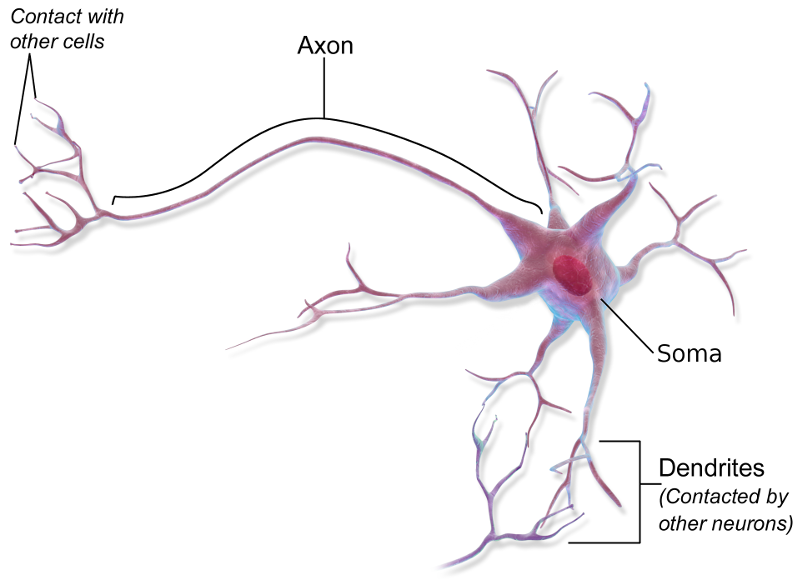
\includegraphics[width=4in]{neuron_small.png}
  \captionb{Cartoon of a neuron.}{
    A neuron receives input from other neurons via synapses on its dendrites.
    The dendrites transmit current to the soma,
    where electrical charge is integrated.
    If the neuron membrane becomes sufficiently polarized,
    it transmits an action potential (\aka/ spike) down its axon.
    This causes neurotransmitter to be released at the synapses,
    which then initiate currents in the dendrites of postsynaptic neurons.
    Image \textcopyright\textcite{BlausenNeuron} with modification, licensed under CC BY 3.0.
    }
  \figlabel{neuron}
\end{figure}

Neurons are only one of the many types of cells in the brain,
but they are the most discussed,
because they are the main computational entities.
Their basic function is simple:
neurons receive input from other neurons,
and if that input excites them sufficiently,
they will fire an action potential (\aka/ spike)
which propagates to other neurons.

A basic cartoon of a neuron is shown in \fig{neuron}.
Neurons can be divided into three parts: the dendrites, the soma, and the axon.
Neurons receive input currents via their dendrites,
which the dendrites then transmit or channel into the cell body,
called the soma.
When a neuron spikes, it sends current down its axon,
causing neurotransmitter(s) to release at the synapses,
which are connections from a neuron's axon
to the dendrites of other neurons.
This neurotransmitter release results in dendritic input currents
in these other connected neurons.

\begin{figure}
  \centering
  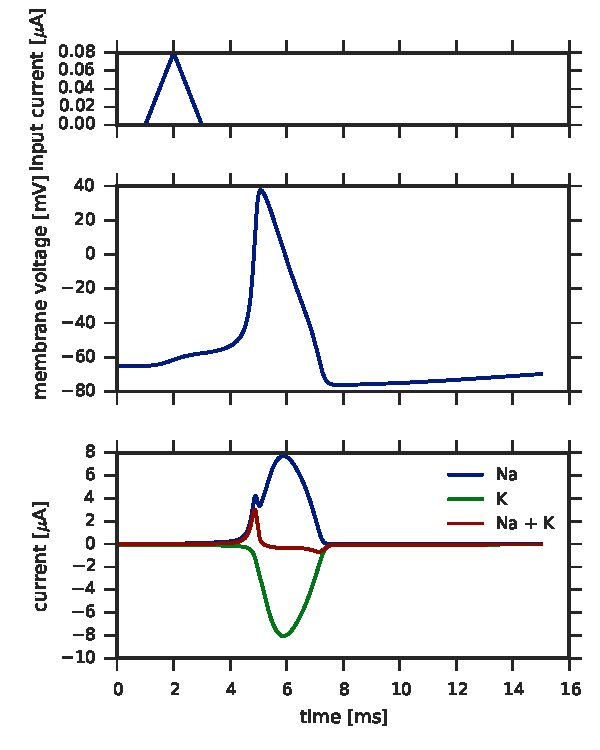
\includegraphics[width=4in]{hh_spike.pdf}
  \captionb{Spiking dynamics of a neuron.}{
    An external input current is applied at the soma of a neuron.
    It causes a slight ($\sim$10 mV) increase in the membrane voltage,
    which triggers a sufficient number of voltage-gated sodium channels
    to initiate a spike.
    The incoming sodium current increases the membrane voltage,
    which opens more sodium channels,
    causing an exponential increase in the membrane voltage
    (the leading edge of the spike).
    As the voltage nears its peak,
    it also triggers voltage-gated potassium channels,
    letting potassium ions out of the neuron and repolarizing it.
    The neuron then enters a hyperpolarized state (below its resting voltage)
    where the potassium channels slowly close
    and the sodium channels are inactivated.
    Only after a period of time (the absolute refractory period)
    can the neuron fire another spike.
    }
  \figlabel{neuron-spike}
\end{figure}

% The soma forms the main body of the neuron.
The soma is the main body of the neuron.
Computationally, it is where all the incoming currents from dendrites
are integrated,
and where the process of creating an action potential begins (\fig{neuron-spike}).
When a neuron is at rest, the soma has a negative charge;
this is called the resting voltage,
and is maintained by ion pumps that maintain a particular concentration of ions
(mostly sodium Na$^+$, potassium K$^+$, and calcium Ca$^{+2}$) inside the cell.
As currents arrive from the dendrites,
they begin to depolarize the cell.
When the voltage in the soma becomes high enough,
it begins to trigger voltage-activated sodium channels,
which allow sodium ions to enter the cell, further depolarizing it.
This process continues until the electrical gradient
due to the increase in sodium ions
opposes the chemical gradient due to the imbalance of sodium
inside and outside the cell.
This gives the neuron a much more positive charge
than when it is at its resting voltage.

This large depolarization also triggers voltage-gated potassium channels,
which begin to let potassium ions \emph{out} of the cell,
helping to repolarize it.
At the same time, the sodium channels inactivate.
The open potassium channels eventually bring the cell to below its resting voltage,
called the hyperpolarized state.
The sodium channels remain inactivated and the potassium channels remain open
for a while after the spike.
The combination of these factors makes it almost impossible
for the neuron to fire during this time;
this is called the absolute refractory period.
The change in ionic concentrations inside the cell is quite small
during a single spike,
but over the course of many spikes,
the ion pumps are needed to maintain the proper concentrations
of sodium and potassium.
Other currents, most significantly calcium currents,
are present in some neurons.

% axons
The rapid depolarization associated with an action potential
not only causes the somatic voltage potential to increase,
but also causes some depolarization in the parts of the axon
nearer to the soma.
This triggers sodium channels in that part of the axon,
resulting in more depolarization and
triggering sodium channels farther down the axon.
In this manner, the somatic spike triggers a voltage wave
that travels down the axon,
eventually triggering the synaptic vesicles near the ends of the axon
and causing them to release neurotransmitter(s).

Axons are responsible for transmitting long-range signals in the brain,
and thus vary widely in length,
depending on whether a particular neuron connects to nearby neurons
or to neurons in another brain area.
To facilitate long-range transmission,
axons are coated in myelin,
a substance composed mainly of lipids and thus a good electrical insulator.
This helps current to propagate down the axon.
The high proportion of fat makes myelin white;
bundles of axons are responsible for the ``white matter'' parts of the brain.
The ``grey matter'' on the other hand
is composed mainly of neuron dendrites, somas, and short-range axons.

% dendrites: active vs passive? role in computation?
Dendrites are thin processes that extend away from the soma
to connect to the axons of other neurons.
Their role is to transmit current from synapses with other neurons to the soma.
They were originally believed to only conduct current passively,
but research has shown that they have active conductance mechanisms
similar to those involved in spike generation and propagation down an axon
\parencite{Mel1994,Johnston1996}.
Dendrites are also traditionally believed to act linearly,
summing together inputs from many synapses across time and space,
and many computational models still treat them as such.
More recent studies \parencite[\eg/][]{Polsky2004} show that signal summation
in dendrites is more complex,
combining linear and nonlinear (sigmoidal) elements.

% synapses
Neurons are connected to one another by synapses,
connecting the axon of the presynaptic neuron
to a dendrite of the postsynaptic neuron.
When the presynaptic neuron spikes,
an electrical pulse travels down its axon to the presynaptic terminals
of all synapses on the axon.
These terminals contain synaptic vesicles filled with neurotransmitter;
the electrical pulse causes the vesicles to release neurotransmitter
into the synaptic cleft,
which is the small area between the presynaptic terminal
and the postsynaptic terminal.
This neurotransmitter activates receptors on the postsynaptic terminal,
which open, allowing current to flow into the postsynaptic cell.
The type of neurotransmitter used by the synapse depends on the presynaptic neuron.
All synapses on a neuron's axon release the same neurotransmitter
or combination of neurotransmitters; this is known as Dale's principle.\footnote{
  When Dale's principle was developed,
  it was believed that each neuron only produced
  one type of neurotransmitter.
  It was only around 1976 that evidence of cotransmission was discovered
  \parencite{Burnstock2004}.
  Nevertheless, Dale's principle remains a good guideline.
  For example, neurons are either exclusively excitatory or inhibitory
  based on the neurotransmitter(s) they release;
  no neurons play both an excitatory and inhibitory role
  to different postsynaptic cells.}


\subsection{Visual system anatomy}

% ventral and dorsal streams

The human visual system performs many functions;
it is not limited to object recognition.
Other functions include estimating object shape, depth, motion (tracking),
and physical characteristics (\eg/ smoothness, hardness) for tasks like grasping,
as well as identifying landmarks and estimating ego-motion for navigation.
The way that many researchers think of the visual system
has been shaped by what is known as the ``two-streams'' hypothesis \parencite{Goodale1992}.
The hypothesis is that the visual system can be roughly divided
into two streams, known as the dorsal and ventral streams.
The ventral stream is sometimes called the ``what'' pathway,
and is associated with object and landmark recognition.
The dorsal stream is sometimes called the ``where'' or ``how'' pathway,
and provides information to inform motor actions related to objects,
such as grasping an object or avoiding an obstacle.


\begin{figure}
  \centering
  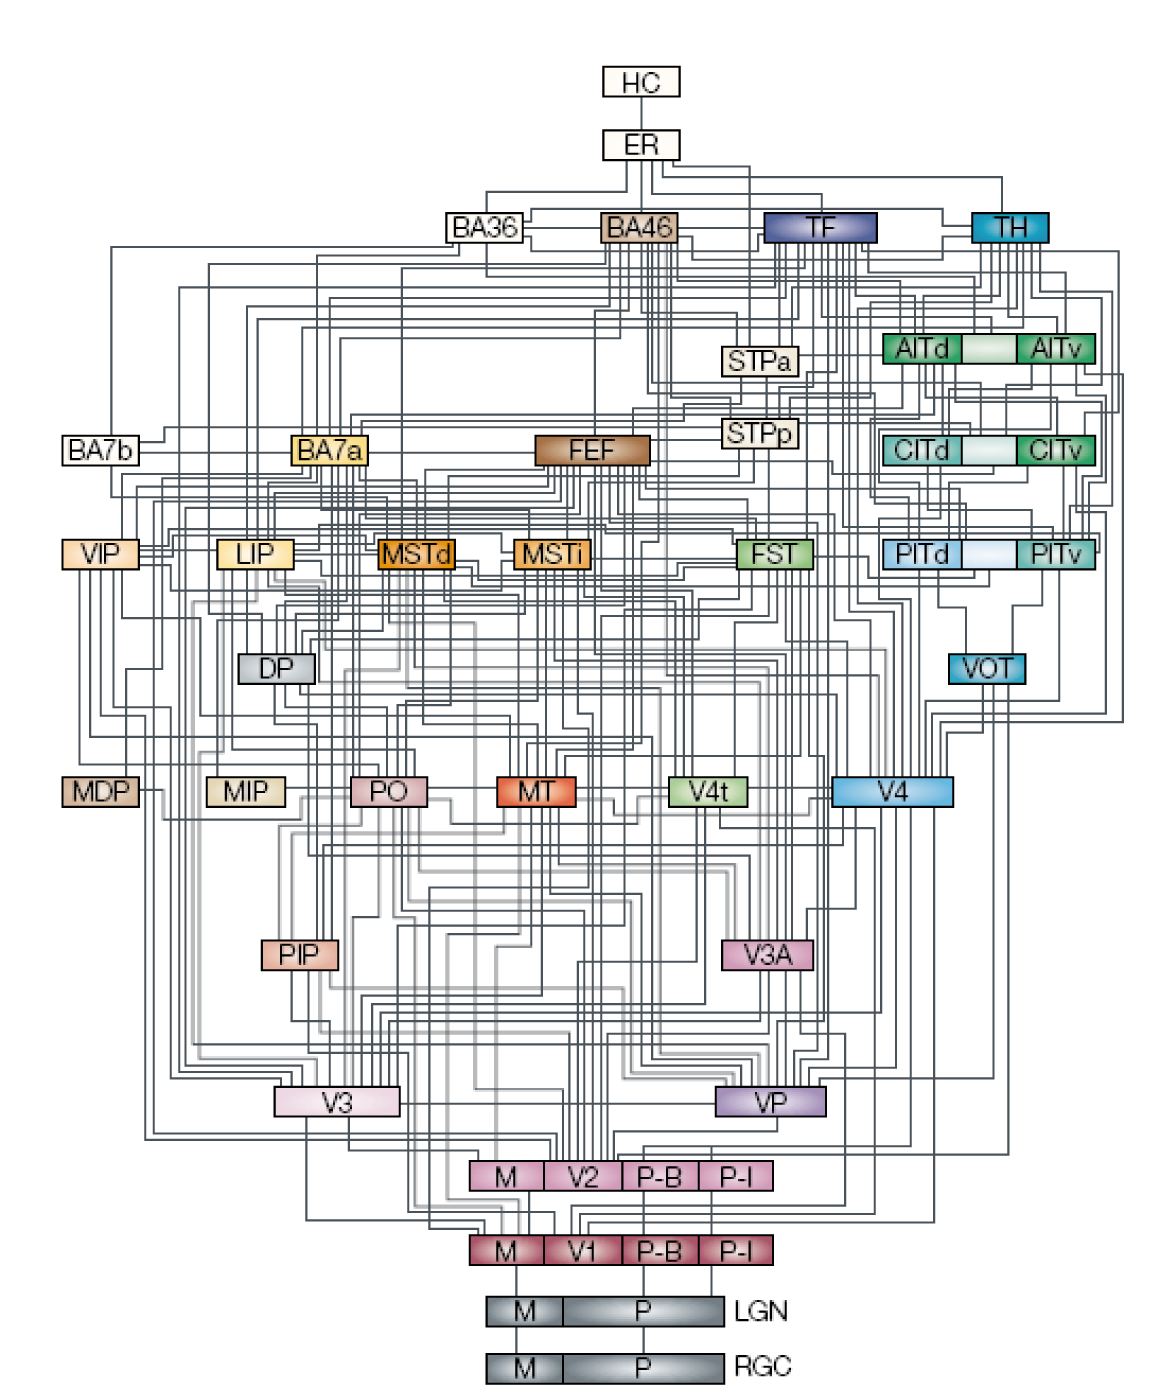
\includegraphics[width=5in]{felleman_vanessen.png}
  \captionb{Hierarchy of the visual cortex of a macaque.}{
    Reproduced from \textcite{Felleman1991},
    depicting connectivity between brain areas in macaque visual cortex.
    Most of the connections have been demonstrated to be reciprocal.
    The ventral stream is on the right,
    culminating in the inferior temporal (IT) areas (AIT, CIT, PIT).
    The dorsal stream is on the left,
    culminating in the intraparietal (IP) areas (VIP, LIP).
    This figure does not show the strength of connections.
  }
  \figlabel{visual-hierarchy}
\end{figure}

% VanEssen visual hierarchy diagram
\fig{visual-hierarchy} is reproduced from \textcite{Felleman1991},
a famous paper examining connectivity in the visual cortices of macaques,
which are known to have similar visual system organization to humans.
The input to the system is at the bottom: the retinal ganglion cells (RGC).
They are already a few steps in from the photoreceptors that transduce
light into neural signals,
and represent a compressed version of the raw photoreceptor input \parencite{Nassi2009}.
The RGCs relay their information through the lateral geniculate nucleus (LGN),
a part of the thalamus.
While some authors do not discuss computational properties of the LGN,
treating it simply as a relay station \parencite[\eg/][]{Nassi2009},
others have found that some LGN cells introduce temporal lags into the signal \parencite{Vigeland2013},
which would be useful for representing motion information \parencite{Adelson1985}.

The next step in visual processing is primary visual cortex (V1).
V1 neurons begin to separate stimuli in a number of ways,
being tuned for changes in contrast (edges), depth, motion, colour, and other properties.
V2 is the next visual layer, it plays a significant role in image segmentation,
specifically representing object contours and border ownership \parencite{Kruger2013}.
It is at this point that the visual system begins to separate
into dorsal and ventral streams.
The ventral pathway continues to V4 and then on to inferior temporal (IT) cortex,
by which point neurons are responsive to object categories.
The dorsal pathway continues to MT and MST---%
both very involved in motion processing---%
before continuing on to intraparietal (IP) cortex
which localizes objects in \ddd/ space and informs motor planning
for actions like grasping.
\textcite{Kruger2013} provides a review of the key visual areas
and their role in computation.

\fig{visual-hierarchy} illustrates how interconnected the visual areas are.
While the dorsal and ventral streams are visible on the left and right, respectively---%
with a high level of connectivity within the streams---%
there is also significant connectivity between the streams.
The functional role of the connections between the streams
remains largely unclear.
Computational models of object recognition---%
including those examined throughout this thesis---%
rarely account for these connections.


\section{Neuron models}

Many of the seminal results in computational neuroscience
are mathematically detailed models of how neurons operate.
Perhaps the most famous of these is the Hodgkin-Huxley model
of the squid giant axon \parencite{Hodgkin1952}.
More recently, the numbers of available neuron models has blossomed,
and current models used in literature range from simple
binary threshold units \parencite{Stocks2001a} (the simplest possible rate-neuron model),
to complex multi-compartmental models
that account for detailed dendritic morphologies \parencite[\eg/][]{Markram2015,}.

For large models of neural systems that hope to reproduce high-level behaviour,
single-compartment neuron models are still the norm.
These models treat the neuron as a single electrical compartment,
combining the dendrites, soma, and axon.
Multi-compartmental models, on the other hand,
model different parts of the neuron as different electrical compartments,
and include equations how the activities of different compartments affect each other.
Models can range from having two compartments
(typically one for the dendrites and one for the soma),
to having thousands of compartments.
The more compartments a model has,
the more computing power it takes to simulate it,
and the more complex its behaviour becomes.
For these reasons, models that seek to reproduce behaviour
predominantly use either single-compartment neurons,
or simpler models that do not model the electrical activity of the neuron at all.
These models are what I will discuss here,
and use throughout the thesis.

Single-compartmental neuron models can be divided along two dichotomies:
1) the rate-based versus spike-based dichotomy;
and 2) the static versus dynamic dichotomy. %\footnote{
  %% There are many other ways to divide and categorize neuron models,
  %% for example single-compartment versus multi-compartmental models.
The rate versus spiking distinction has to do with whether
the output of the neuron model is a continuous value (a firing rate)
or a discrete value (a spike).
Most neurons in mammalian cortex communicate via spikes,
so spiking neuron models are typically considered more physiologically realistic.\footnote{
  There are limited places in the mammalian brain---%
  for example horizontal cells in retina---%
  where neurons communicate via gap junctions,
  and thus could transmit something more akin to a continuous value
  than a discrete spike.}

The static versus dynamic distinction denotes whether the model has
internal dynamics,
such that the output at the current point in time is conditional in some
respect on the time history of the neuron,
or static, such that the output is completely independent of the past
and only dependent on the instantaneous neuron input.
Dynamic neuron models have some form of state,
that is internal variables that evolve over time,
and are not directly computable from the present input to the model.
They are typically expressed using differential equations.
For static models, the output is a function of the current input only,
and thus they do not require differential equations to express them.

% describe rate response function (I-F curve)
It is important to note that the static/dynamic dichotomy does not necessarily
refer to whether the neuron is being used as a static nonlinearity
(evaluated at a single point in time on an input \emph{value})
or as a dynamic nonlinearity (evaluated over a period of time on an input \emph{signal}).
Static neurons can be evaluated dynamically,
simply by evaluating them (independently) on the input value at each successive point in time.
For dynamic neurons, however, there is no general way to evaluate them statically,
since their input at any point in time depends on their internal state,
which is a dynamic process that evolves over time.
For some dynamic neuron models,
we can determine a firing rate response curve
(\aka/ I-F response curve, rate response function),
which maps every constant value for the input current
to a constant firing rate output.
This can be determined analytically (\eg/ \eqn{lifrate}),
or empirically by applying a constant input current
and measuring the rate of the output spikes
(this can even be done in real neurons in vitro).
Many neuron models will not output spikes at a constant rate,
even for a constant input,
due to changing internal dynamics.
For these neuron models,
the rate-response function only captures part of the model,
and will be different depending on the state of the model
and how it is measured or calculated.


\begin{table}
  \centering
  \begin{tabular}{l|l|l}
            & \multicolumn{1}{|c}{\textbf{Rate}}
            & \multicolumn{1}{|c}{\textbf{Spiking}} \\\hline
    \textbf{Static}
      & Sigmoid                   & Poisson spiking              \\
      & Rate LIF                  &                              \\\hline
    \textbf{Dynamic}
      & Adapting rate LIF         & LIF                          \\
      & Sigmoid with state        & Hodgkin-Huxley               \\
  \end{tabular}
  \captionb{Rate vs. Spiking and Static vs. Dynamic neuron model dichotomies.}{
    Neuron models can either transmit information via continuous firing rates (rate-based),
    or via discrete spikes (spike-based).
    They can either have no internal state (static),
    or have their response affected by internal dynamical systems (dynamic).
    }
  \tablabel{neuron-dichotomies}
  %% \vspace{6pt}
\end{table}

\tab{neuron-dichotomies} shows how a few example neuron models fall across
these dichotomies.
In the static rate category, we have models that take in
a continuous value and output a continuous function of that continuous value.
This includes most of the nonlinearities used in machine learning
(such as sigmoids or rectified linear units),
as well as the analytic firing rate for the LIF neuron model (see \scn{lif}).
In the static spiking category, we have models that output a discrete (binary)
function of their continuous input.
This is mainly Poisson-spiking neurons,
which fire probabilistically based on their instantaneous firing rate,
such that the probability of firing at the current time is
independent of past firings.\footnote{
  Poisson spiking can also be applied to a dynamic rate model,
  such that the probability of spiking is independent, but the spike rate is a
  dynamic process \parencite[\eg/][]{Lillicrap2016}.}
Dynamic rate models have an internal state that also affects their continuous output,
in addition to the input.
This includes the analytic LIF rate model with adaptation,
which has an internal adaptation parameter that grows when the neuron is active
and discounts the firing rate.
It also includes sigmoid neuron models that have an underlying voltage
that is dynamically related to the neuron inputs;
such models have recently been applied by \textcite{Guergiuev2017}
when learning deep networks subject to biological constraints.
Finally, the dynamic spiking category includes the LIF neuron model,
as well as the Hodgkin-Huxley model,
as well as more complex multi-compartmental models.

Within the category of spiking models,
we can further distinguish between
models that output instantaneous spikes (\eg/ LIF),
and models that output spikes which vary across time (\eg/ Hodgkin-Huxley).
Another possible distinction would be between models
that output stereotyped spikes,
where the size of each spike is exactly the same,
and those that output variable-sized spikes.
Models of cortical neurons that output instantaneous spikes (\eg/ LIF)
almost always output stereotyped spikes.
This is because spikes in cortical neurons are nearly identical
in terms of magnitude, duration, and shape,
and it is widely believed that none of these factors carry information.
Even among models that have spikes that vary across time (\eg/ Hodgkin-Huxley),
the spike magnitude, duration, and shape are quite consistent between spikes.
Therefore, most spiking cortical neuron models have stereotyped spikes.
Modelling the spike separately from the rest of the neural dynamics
allows for a separation of time scales;
the result is that extra computational resources are not required
to model the spike trajectory,
the details of which are stereotyped and thus of little interest \parencite{Abbott1999}.


\subsection{The integrate-and-fire neuron model}

The integrate-and-fire (IF) neuron \parencite{Lapicque1907}
was one of the first computational models of a neuron.
This model was developed before researchers were able to measure
the electrical and chemical changes happening in a behaving neuron,
and is based simply on the idea that the neuron membrane
can be modelled as a capacitor that stores charge over time \parencite{Abbott1999}.
As the name implies, the IF model has two main behaviours:
1) it integrates current over time (by means of the capacitor);
and 2) when the voltage has reached a threshold, it fires.
Additionally, the model may or may not include a leak term:
a resistor in parallel with the capacitor that allows charge
to ``leak'' out over time.
The model with leak term is typically referred to
as the leaky integrate-and-fire (LIF) model.
While ``integrate-and-fire (IF) model'' can refer to either the leaky or non-leaky model,
in this thesis I will use it to refer specifically
to the non-leaky version of the model.


\subsubsection{The non-leaky integrate-and-fire (IF) model}
\scnlabel{if}

We wish to identify how the neuron's membrane voltage evolves over time,
and from this identify when the neuron spikes.
The charge $Q$ across a capacitor is given by $Q = VC$,
where $V$ is the voltage across the capacitor and $C$ is the capacitance.
Differentiating this with respect to time,
we find that the membrane voltage $V(t)$ of the neuron is governed by
\begin{align}
  C \diff{V(t)}{t} = J(t)
  \eqnlabel{ifdiff}
\end{align}
where $J(t)$ is the input current to the neuron over time,
and $C$ is the membrane capacitance.
(Remember that current is the time derivative of charge.)

\eqn{ifdiff} shows that the IF neuron simply integrates
the input current over time.
We still need to identify when the neuron spikes.
To do this, we define a threshold voltage $\Vth$.
When the voltage passes this threshold, the neuron fires.
This comes from a key fact in neurophysiology:
once the neuron voltage passes a threshold,
the neuron begins firing a spike,
and once this firing process begins,
it is almost impossible to reverse.

Finally, we define a reset procedure:
once the neuron has fired a spike,
the membrane voltage is reset to the resting potential $\Vrest$.
This again comes from physiology:
after a neuron spikes,
other ionic currents (typically potassium)
kick in and bring the membrane voltage back towards the resting potential.

Some integrate-and-fire models may also model an absolute refractory period:
a time $\tref$ for which the voltage is held at the resting potential $\Vrest$
after a spike.
In cortical neurons, post-spike potassium currents are strong enough
that it is practically impossible for the neuron
to fire another spike for a period of time.
This time is called the absolute refractory period.
We model this by holding the membrane voltage at $\Vrest$
for a length of time $\tref$.


\subsection{The leaky integrate-and-fire (LIF) model}
\scnlabel{lif}
% Citation: Knight1972
% Citation: Gerstner and Kistler 2002? Koch1999?

The leaky integrate-and-fire (LIF) model \parencite{Lapicque1907,Knight1972,Koch1999}
takes one additional physiological factor into account:
Neuron membranes are not perfect capacitors,
rather they slowly leak current over time,
pulling the membrane voltage back to its resting potential.
Thus, we model the membrane as a capacitor and resistor in parallel.
This gives the neuron some ``forgetting'':
in the absence of any input, the membrane voltage will return to its
resting potential.

The LIF dynamics are captured by the following equation:
\begin{align}
  C \diff{V}{t} = -\frac{1}{R}(V - \Vrest) + J(t)
  \eqnlabel{lifdifffull}
\end{align}
where $R$ is the membrane resistance,
and the other parameters are the same as in the IF model.
The resetting procedure is also identical to the IF model.


\subsubsection{Normalized model}

The LIF model has a number of parameters:
$C$, $R$, $\Vrest$, $\Vth$.
We can normalize the model to reduce the number of parameters,
while keeping the full dynamics of the original model.
Specifically, we manipulate the model
so that the normalized voltage lies in the range $[0, 1]$,
with a normalized resting potential of zero
and normalized firing threshold of one.

First, we multiply \eqn{lifdifffull} through by $R$:
\begin{align}
  \taurc \diff{V}{t} &= -V + \Vrest + R J(t)
\end{align}
where $\taurc = RC$.
Then, letting $\bar V = (V - \Vrest) / (\Vth - \Vrest)$
and $\bar \Vrest = \Vrest / \Vth$:
\begin{align}
  \taurc (\Vth - \Vrest) \diff{\bar V}{t} &= -(\Vth - \Vrest) \bar V + R J(t) \nonumber\\
  \taurc \diff{\bar V}{t} &= -\bar V + \frac{R}{\Vth - \Vrest} J(t) \nonumber\\
  \taurc \diff{\bar V}{t} &= -\bar V + \bar J(t)
  \eqnlabel{lifdiff}
\end{align}
where the firing threshold for the new equation is $\bar \Vth = 1$,
the voltage is reset to $\bar \Vrest = 0$,
and $\bar J(t) = \frac{R}{\Vth - \Vrest} J(t)$.
Observe that $\bar J(t)$ is simply a linear transformation of $J(t)$.
Thus, \eqn{lifdiff} retains all the dynamics of \eqn{lifdifffull} for a scaled input,
but with only one parameter $\taurc$.

Note that $\bar V$ and $\bar J$ are both unitless quantities.
In this thesis, we work exclusively in this unitless space,
and often refer to $\bar V$ and $\bar J$ simply as $V$ and $J$,
despite the fact that these quantities are not actually voltages or currents.
This simplifies the mathematics,
without limiting the generality of our models.


\subsubsection{Rate equation}

\eqn{lifdiff} describes exactly when the model neuron will spike
for a given input current $J(t)$.
However, sometimes we only care about the spike rate,
that is, how many times per second the neuron will spike
for the given input current.

For the LIF model, we can determine the analytical firing rate
for a constant input current.
We do this by determining the inter-spike interval (ISI),
that is the time between one spike and the next.
Then, the firing rate is given by the inverse of the ISI.

Given a constant input current $J(t) = j$,
we can solve \eqn{lifdiff} to find the neuron voltage over time:
\begin{align}
  V(t) = (V(0) - j) e^{-t / \taurc} + j
  \eqnlabel{lifvoltage}
\end{align}
assuming no spikes are fired.
We want to know how long it takes for the voltage to rise from $V(0) = 0$
to $V(t) = 1$.
This will only occur if $j > 1$.
Substituting into \eqn{lifvoltage} and solving for $t$:
\begin{align}
  t &= -\taurc \log\left(-\frac{1}{j}\right) \text{ .}
\end{align}
Adding in the refractory period and inverting,
the spike rate $r$ for the LIF neuron is given by
\begin{align}
  r = \frac{1}{\tref - \taurc \log\left(1 - \frac{1}{j}\right)}
  \eqnlabel{lifrate}
\end{align}
if $j > 1$, and zero otherwise (since the neuron is silent).


\section{Synapse models}
\scnlabel{synapses}

In addition to modelling internal neural dynamics,
it is also important to model the dynamics of the synapses
that connect neurons to one another.
The most significant functional effect of synapses is
as a low-pass filter on the spikes passing through them.
A spike in the presynaptic neuron elicits an extended current pulse
in the postsynaptic neuron.
This pulse can be viewed as a low-pass-filtered version
of the presynaptic spike.

The simplest model of a synapse is as a first-order lowpass filter.
The impulse response of a filter describes how the filter responds to
an infinitesimally short input of unit integral, called an impulse.
This idealized impulse is also reasonable model of a spike,
thus the impulse response also describes what the postsynaptic current
will look like in response to a presynaptic spike.
The impulse response of the first-order lowpass filter is:
\begin{align}
  h(t) = \frac{1}{\taus} e^{t / \taus}
  \eqnlabel{expo-synapse}
\end{align}
where $\taus$ is called the synaptic time constant,
and relates to the length of time the postsynaptic current is spread over.
Since the impulse response is an exponential function,
it is known as the exponential synapse model.

\textcite{Mainen1995} found that a second-order lowpass filter
is a better model of a synapse.
The impulse response of this filter is given by
\begin{align}
  h(t) = \frac{t}{\taus^2} e^{t / \taus} \text{ .}
  \eqnlabel{alpha-synapse}
\end{align}
This function is known as the alpha function,
and thus the model is called the alpha synapse model.
%% Again, $\taus$ is the only parameter of the model,

Both of these models are current-based synapse models,
meaning that they explicitly model the current that results from a spike
in the postsynaptic neuron.
Other current-based synapse models exist;
a popular one is the double-exponential model,
which is similar to the alpha synapse but with two time constants,
allowing more control over the rise and fall of the impulse response.\footnote{
  The double-exponential model with both time constants set to the same value
  reduces to the alpha synapse.}
Many of the other, more realistic synapse models are conductance-based,
meaning that they model the conductance of the neural membrane at the synapse.
The current into the neuron depends on both the conductance
and the voltage across the membrane;
the latter changes as the synapse becomes active.


\section{Rate codes, population codes, and timing codes}
\scnlabel{codes}

%  - Difference between rate and temporal codes is actually in the freq.
%    of fluctuations in the firing rate. Not related to independence.
%  - In a pure rate code, Poisson spiking would be equivalent to constant-ISI
%    spiking, whereas in \eg/ an NEF network, the fluctuations produced by
%    Poisson spiking could be interpreted as meaningful by downstream neurons.
%  - My idea: for a particular (constant) stimulus, a rate code would have
%    constant FR, whereas a timing code would have fluctuating FR?
%  - Example of distinction: rate code for stimulus intensity versus rank-order
%    timing code (\eg/ Bhattacharya2010). Rate code still has some temporal
%    aspects, for example neurons with higher input intensity will fire first.
%    This is what allows first-to-spike metrics to work even in networks trained
%    with rate neurons.
% difference between rate and timing codes is whether changing phase of
% regular spike train affects results?

One of the aims of computational neuroscience has been to determine
how the brain represents---or encodes---information.
To this end, researchers have proposed a number of different
\emph{coding schemes} that neurons could use to encode information.


\subsubsection{Rate versus timing codes}

One dichotomy differentiates between rate coding and temporal coding.
In a rate code, only the firing rate (\ie/ number of spikes)
of a neuron over a period of time matters.
An archetypal example of a rate code
is motor neurons in the peripheral nervous system.
A muscle's contraction is based on the number of spikes per unit time,
thus only the rate of motor neuron spikes is important \parencite{Gerstner1997}.
In a temporal code, the \emph{time} of individual spikes is also important.
An archetypal example of a timing code is in the early auditory system \parencite{Gerstner1997},
where precise spike timing helps to localize sounds \parencite{Chase2006}.

The exact definitions of rate and temporal codes are not clear,
and vary from author to author \parencite{Dayan2001}.
For example, a neuron may fire a number of spikes in quick succession,
and then be silent.
Compare this with a second neuron, that fires the same number of spikes,
but spread evenly over a given period.
One way to view this is that both neurons have the same firing rate,
but the one has all its spikes near the start of the period,
in which case the timing of the spikes is important.
An alternative view says that the \emph{instantaneous} firing rate of
the first neuron changes over the period,
whereas that of the second neuron remains constant,
and it is only this instantaneous firing rate that matters.
This points to one problem with only looking at the overall firing rate
(\ie/ number of spikes) of a neuron over a period:
it is not clear what period we should count over.
In real neurons,
the period of time that matters for counting spikes depends on parameters like
the membrane time constant $\taurc$ of the postsynaptic neuron.

For this reason, neuroscientists will often distinguish
between rate and timing codes
based on the frequency of the changes in the instantaneous firing rate.
If the rate fluctuates rapidly,
and these fluctuations contain information about the stimulus
(they are not simply spurious variation or ``noise''),
then the code is said to be temporal; otherwise it is a rate code.
Again, there is ambiguity as to how fast the firing rates must fluctuate
to be considered temporal.
One way to define this is relative to the stimulus.
Fast-changing stimuli can trigger fast changes in the firing rate of neurons,
whether they are using a rate code or a temporal code.
If we define a temporal code as having meaningful firing rate fluctuations
at a faster time scale than changes in the stimulus,
we can differentiate between codes that have fluctuations
because they are using them for coding,
and those that simply have fluctuations triggered by the stimulus.
By this definition,
neurons using a temporal code will have a fluctuating firing rate
in response to a constant stimulus,
whereas neurons using a rate code will have a non-fluctuating firing rate.


\subsubsection{Population coding}

Both rate codes and temporal codes describe
the encoding properties of individual neurons.
We can also ask about the coding properties
of a group (\aka/ population) of neurons.
The concept of \emph{population coding} describes when a representation
is distributed across many neurons in a population,
such that the represented value cannot be decoded from only the activities
of a few neurons.

To illustrate, the simplest way of extrapolating the idea of rate or temporal
coding to more than one neuron
would be to have many neurons all implementing the same code.
That is, all neurons will fire similarly when representing a given value
(they have similar \emph{tuning}).
This creates a large degree of redundancy between neurons.
Instead, population coding has each neuron represent a different aspect
of the represented value.
For example, if we want to represent head direction,
we have neurons that represent the head fully turned to the left,
others that represent fully turned to the right,
and still others for centred, and others for values in between.
The direction that a neuron is most active for is called its preferred direction.
Each neuron has some variance, that is, it will fire for head directions
close to its preferred direction, as well.
The farther the actual head direction is from a neuron's preferred direction,
the less it will fire.
By using the activities of all neurons in the population,
we can decode the head direction quite accurately.

At the population level,
we can distinguish between codes that take advantage of synchrony between neurons
and those that do not.
This can be facilitated for example by \emph{coincidence detection},
where a postsynaptic neuron will only fire if the spikes of two
of its input neurons are coincident,
that is, they fall within the same (small) temporal window.
Here, we see another distinction between temporal and rate coding schemes:
Only temporal codes can take advantage of correlations
between individual spikes of neurons.
Rate coding schemes, on the other hand,
can only take advantage of synchrony between neurons in terms of
synchronized fluctuations of their instantaneous firing rates,
since they do not have the temporal precision to co-ordinate individual spikes.

%% Therefore, the fundamental distinction between rate and temporal codes
%% is that in a rate code, the whole system will function as well or better
%% if all spiking neurons are replaced with ideal rate-based approximations.
%% With temporal codes, the timing of individual spikes matters,
%% so they will no longer function properly when using rate-based neuron models.


%% \subsubsection{Sparse and distributed representations}

%% When discussing coding at the population level,
%% another important distinction is between sparse and distributed representations.


\section{The Neural Engineering Framework (NEF)}
\scnlabel{nef}

The Neural Engineering Framework (NEF, \textcite{Eliasmith2003}
is a theory that connects neural-level computations
with higher-level algorithmic descriptions.
Specifically, it describes how neurons can perform vector computations,
which can then be built upon to create increasingly complex systems,
for example Spaun \parencite{Eliasmith2012}.
It has three main tenets:
1) representation, how neurons represent a real-world value;
2) transformation, how neurons compute (static) functions on represented values;
and 3) dynamics, how neurons can implement dynamical systems or functions.

The core of the Neural Engineering Framework is based on population coding.
Specifically, it extends a method proposed by \textcite{Salinas1994}
on how linear least-squares can be used to find linear decoders for a
population of neurons.
This idea can be summarized succinctly as
``nonlinear encoding, linear decoding''.
Here, we will focus on the first two tenets: representation and transformation.


\subsubsection{Representation}

The core idea behind the NEF is that a ``population'' of neurons
can be viewed as representing some value.
This could either be a value in the real world
(such as an animal's current head direction)
or a purely internal value
(such as the sum of three and seven when mentally computing $4 \times (3 + 7)$).
In the core NEF, each population represents a vector $\vect x$,
but this can be extended to representing things like
scalar- and vector-fields, too.

Each neural population has a set of \emph{encoders} $\mat E$,
which map from the space of values that the population can represent
(called the state space, of dimension $d$)
to the space of neural activities (called the neuron space, of dimension $n$).
The mapping is nonlinear:
\begin{align}
  a_j(\vect x) = G_j\left(\alpha_j \sum_i E_{ji} x_i + \beta_j\right)
\end{align}
where $\vect x$ is the vector value that the population is encoding,
$a_j$ is the activity of neuron $j$,
$G_j(\cdot)$ is a rate-based neural nonlinearity
transforming input currents into firing rates,
$\mat E$ is a $n \times d$ matrix of encoders,
and $\alpha_j$ and $\beta_j$ are scalar gain and bias terms, respectively.
Often, neurons in the NEF are modelled as LIF neurons,
in which case $G_j$ is given by \eqn{lifrate} for all neurons.

To decode information from the population,
we find linear decoders $\mat D$,
which when multiplied by the neural activities $\vect a(\vect x)$,
will yield our state-space value $\vect x$.
Typically, we choose decoders that minimize the squared error
$\|D \vect a(\vect x) - \vect x\|_2^2$.
Ideally, we would minimize this across all possible values of $\vect x$;
in practice, we sample the space of $\vect x$ at $m$ points,
called evaluation points.
Given our $m \times d$ matrix of evaluation points $\mat X$,
and the corresponding neural activities at each evaluation point $\mat A$,
we can find the least-squares optimal decoders as
\begin{align}
  \mat D = (\mat A^T \mat A)^{-1} \mat A^T \mat X \text{ .}
\end{align}
In practice, some neurons may have similar activity patterns,
making this an ill-conditioned problem.
Additionally, we typically want to put a penalty on large decoders
to reduce the effects of variability in the spiking neurons on the decoded value.
To address these problems, we typically regularize the problem
(see \scn{dec-regularization}).


\subsubsection{Transformation}

Since the number of neurons in the population $n$
is typically much larger than the number of dimensions $d$ in the encoded vector $\vect x$,
the neural population not only contains information about $\vect x$,
but also about possible functions of $\vect x$.
We can decode a function $f(\vect x)$ from the population
by finding decoders $D_f$ that minimize the squared error
$\|D_f \vect a(\vect x) - f(\vect x)\|_2^2$.
This results in a similar least-squares optimization problem as before,
but replacing the matrix of evaluation points $\mat X$
with a matrix of targets $\mat Y$.
This method can be used to decode arbitrary functions from the population.
The accuracy with which a given function can be decoded depends
on the characteristics of the function
(\eg/ higher frequency changes are more difficult to decode),
the tuning curves of the neurons,
and how these two factors relate.


\subsubsection{Discussion}

%%  - encoding/decoding model is rate-based. This is not to say NEF models
%%    use only rate coding; firing rates can change quite quickly, thus
%%    exhibiting something more akin to temporal coding. However, the
%%    fundamental model is of neurons as rate-based. Furthermore, all neurons
%%    are treated as independent. Synchrony between neurons is not exploited,
%%    in fact it is discouraged, since it would cause correlated noise between
%%    neurons, and here we treat all spiking ``noise'' as independent.
One observation about the encoding model is that it is rate-based.
To find the decoders, we use the rate response function of the neurons.
This does not mean that NEF models use traditional rate coding;
firing rates can vary quite quickly,
and one can design models---for example an oscillator---%
where neurons fire in quick bursts, for which the timing is important.
NEF networks cannot take advantage of synchrony between neurons;
any correlations between neural firing will only result in
increased variability (noise) in the decoded output.
Furthermore, NEF networks function equally well or better
when rate-based neurons are used instead of spiking neurons.
This suggests that these networks use what is fundamentally a rate code,
albeit one that can change quickly.

%%  - Neurons are heterogeneous, play large role in what functions we can decode
An important aspect of NEF networks is that neurons are heterogeneous
in terms of their encoders and biases,
and thus respond differently to input stimuli.
This heterogeneity is what allows neurons to not only encode
different aspects of their input signals
(something that can also be done with noisy homogeneous neurons, see \textcite{Hunsberger2014}),
but compute nonlinear transformations of these signals.
The exact nature of this heterogeneity has a significant effect
both on what signals can be represented,
and what transformations can be computed.
Representation and transformation do not always go hand in hand;
for example, a population whose neurons are all tuned to the sum of two inputs
is not able to represent the individual signals,
but is able to compute a transformation such as the square of their sum.
What types of heterogeneity are best for computing particular functions
has not been well examined.
\scn{nef-encoding} will look at what types of encoders are good
for performing object classification tasks.


\section{Neuromorphic hardware}

Neuromorphic engineering is broadly concerned with creating artificial systems
that work like biological neural systems,
particularly in terms of their physical implementation.
The term was coined by Carver Mead in the late 1980's,
and refers to both digital and analog hardware
that is organized in a more brain-like manner
than traditional computer hardware \parencite{Mead1990}.
One of the core ideas behind neuromorphic systems
is parallel distributed processing;
neuromorphic systems organize computations at a neural level,
and pay particular attention to facilitating fast communication between
neural processing units.
This differs from other parallel distributed systems
like graphics processing units (GPUs),
which are typically optimized for independent parallel computations
and have poor communication between units.

Neuromorphic systems can be either digital or analog.
Digital systems, such as SpiNNaker \parencite{Furber2013} and TrueNorth \parencite{Merolla2014},
use the same basic components as traditional computers
(even using the same chips in some cases),
but optimize connectivity and communication for neural systems.

Analog systems embrace the fundamental analog nature of electrical systems,
and construct systems using core components that are analog instead of digital.
On some systems (\eg/ NeuroGrid, \textcite{Benjamin2014}),
neurons are modelled using analog circuits.
This is extremely energy efficient compared with digital circuits,
since as little as one RC circuit can represent
and update a neuron membrane voltage with leak,
which would require multiple bits and multiple updates per time step
on digital hardware.


%%%%%%%%%%%%%%%%%%%%%%%%%%%%%%%%%%%%%%%%%%%%%%%%%%%%%%%%%%%%%%%%%%%%%%%%%%%%%%%%
\chapter{Machine Learning}
\chplabel{ml}

The field of machine learning (ML) is concerned with how computers
can learn to perform various tasks,
and is a sub-branch of the field of artificial intelligence (AI).
AI addresses the problem of how to get machines
to do ``intelligent'' things.
Initial approaches were focused on how to program this desired intelligence,
and grew out of fields like optimization and control theory.
One drawback to this initial approach is that the programmer would need
to be able to formulate specific instructions telling the machine how to
act in different circumstances.
This led to \emph{rule based systems},
which are successful at some tasks,
but for other tasks it is incredibly difficult to determine
an explicit set of rules to guide behaviour.
For example, how would you choose rules to differentiate between
the visual stimuli of a cat and a dog?
You can begin by trying to make rules to distinguish between different
characteristic features;
for example, differences in the appearances of ears, noses, mouths, and so on.
However, it is very hard to come up with rules that cover
even the majority of situations,
and promising rules may prove to be fragile to changes in viewing angle,
viewing distance, or environment.
The reason it is so difficult to come up with rules for this situation
is that recognizing objects is something that people do subconsciously.
We cannot think of explicit rules because we do not have them,
not in the same way that we have rules for doing mental math, for example.
Rather, our visual system has been bombarded over time with
millions of seconds of ever-changing stimuli,
and learned to process these stimuli in such a way that we can do everything
from distinguishing different types of objects,
to judging the depths of obstacles in our environment.

Machine learning was born when researchers started asking whether
we can get machines to learn these implicit ways of operating, too.
Rather than programming in a set of rules or commands,
can we have the machine learn its own program, so to speak.
This is often described as a \emph{data-driven} approach:
give the machine a general structure for the problem,
and a lot of data,
and let it \emph{learn} a way to solve the problem.
Empirically, there is no general structure that works well across
different types of problems,
and much of the research in machine learning goes into
what kinds of structures, and what kinds of learning procedures,
work best for a particular problem or group of problems.

One of the most prolific sub-fields in machine learning has been that of
artificial neural networks (ANNs).
ANNs take inspiration from the brain
by defining a ``neuron'' (or node) as the fundamental unit of computation.
Typically in an ANN,
a neuron will take a (linearly) weighted set of inputs,
and then pass this through a (static) function to obtain the neuron's output.
An ANN can have many such neurons,
and much of machine learning is concerned with how to adjust the parameters of the model
(typically the weights on each neuron's inputs)
such that the model as a whole obtains the desired output.
Additional difficulty comes from the fact that we do not want our system to
only perform well on the stimuli that we train it on,
but also on stimuli that it has not seen before.
It is relatively easy to memorize a set of desired input and output pairs,
and given one input produce the desired output.
It is much more difficult to generalize what has been learned to new
stimuli in an ``intelligent'' manner,
and this generalization problem is the core problem of machine learning.

This chapter will summarize the ANN sub-field of machine learning,
particularly those aspects concerned with solving object classification problems,
which have been one of the core problems used to demonstrate the abilities of ANNs.
I will briefly summarize the development of ANNs,
before focusing on some of the key pieces related to their modern practice.


\section{Machine learning basics}

Early efforts in artificial intelligence were driven by theory:
Researchers would take what they knew about the problem
and use it to develop algorithms and rules to address that specific problem.
It soon became clear that for many problems,
it was extremely hard to explicitly write out
all the rules that would be needed to solve that problem.
For example, traditional computer vision approaches have relied on
detecting specific hand-defined features in an image.
This can work reasonably well for problems like tracking moving objects,
where simple features can be combined with the principles of motion
to keep track of an object from one frame to the next.
For problems like object recognition, however,
it is almost impossible to explicitly define good features and rules.
To tell a cat from a dog from a boat from a truck,
one would need to design feature detectors for things like ears, eyes,
sails, wheels, and so on,
and then define rules about how these relate for different types of objects.
One would quickly have hundreds of features and rules,
and would have to hand-tune each one to work properly on the data.


\subsection{Goal}

Machine learning takes a data-driven approach.
Rather than explicitly define good features and rules,
the goal of machine learning is to \emph{learn} them from the data.
Specifically, we want to learn a function
that is able to perform the desired computation on new data points
(\ie/ different from the ones used for learning).
This is called \emph{generalization},
and is what allows a machine-learning system to be deployed in the world.
If the system only performed well on stimuli that it has already seen,
then unless we can show it every possible stimulus it will ever see
(which is impossible for high-dimensional stimuli, such as images),
the system will always perform poorly on new stimuli.
If, however, the system is able to generalize
from the training stimuli to similar stimuli,
then it can perform well on novel stimuli too.

The desired computation of a machine learning system
is defined implicitly both by the available training data,
and by the learning paradigm.
The latter is the focus of the next section.


\subsection{Learning paradigms}
\scnlabel{learning-paradigms}

The learning paradigm defines both what information
we have available to learn from,
and what the desired output of the system is.
There are three main paradigms:
supervised learning, unsupervised learning, and reinforcement learning.
The main way these paradigms differ is in terms of what type of error signal
is provided to the learner.

In supervised learning,
we have both the desired inputs and outputs to the system,
and we wish to learn an input-output mapping.
It can be separated into regression problems, which have continuous outputs,
and classification problems,
which have binary outputs (representing membership in different categories).
The error signal is defined based on how far the system's output
is from the desired output.

In unsupervised learning,
we have input data (\eg/ images), but no desired outputs.
Rather, we implicitly define an output based on the input data.
Types of unsupervised learning include
clustering, which attempts to group the input data into sets,
and dimensionality reduction, which attempts to represent the data using
fewer dimensions than the original representation.
The error signal is defined based only on the input.
For example, for dimensionality reduction,
we wish to create a system that can take an input and represent it with fewer dimensions,
but still re-create the input from this representation.
In this case, the error signal could be how far this re-creation
is from the original input.

Finally, reinforcement learning has a more temporal aspect:
given a current state of the environment,
the system must choose an action,
which determines (perhaps probabilistically) the next state of the environment.
Certain environmental states are rewarded,
while others are punished (negative reward) or neutral (no reward).
The system wants to achieve maximum total reward over time.

While these are the main categories of learning problems typically studied in ML,
this is not an exhaustive list.
Other paradigms exist, such as semi-supervised learning,
where some data points are labelled and others are not
(thus falling between supervised and unsupervised learning).
Supervised learning is still the dominant paradigm in object recognition.
As datasets grow larger and thus the cost
of having fully labelled datasets is higher,
object recognition will likely move to incorporate more
semi-supervised and unsupervised methods,
and even reinforcement learning
(\eg/ when object recognition is part of a larger problem,
such as winning at video games \parencite{Mnih2013}).
That said, this thesis focuses only on supervised learning.

Within supervised learning, there are two traditional kinds of problems:
regression problems and classification problems.
The difference is in the output of the system.
Regression systems output one or more continuous values
(computing a vector-valued function on the input),
whereas classification systems compute a single discrete-valued output
(representing the class-label of the input).
More recently, there has been increased interest
in problems that go beyond these two categories.
One example is predicting multiple labels for an image---%
for example corresponding to many objects in an image---%
or determining verb-like correspondences between objects \parencite{Karpathy2015}.
This can be expanded to generating captions for images,
where the model output is a sentence describing the image
\parencite{Karpathy2015,Xu2015}.
This thesis will focus on classification problems,
which is the typical paradigm used when performing object classification.


\subsection{Basic components}

Each machine learning system can be described in terms of four components:
\begin{enumerate}
  \item Dataset/Problem:
    The set of data that is available to learn from,
    which implicitly defines the problem. In the case of supervised learning,
    this is a set of input/output pairs; in unsupervised learning, it is only
    inputs; in reinforcement learning, it is an environment that defines the
    set of possible states and which states produce which rewards.
  \item Architecture:
    How our learner is constructed,
    namely what are the parameters being learned,
    and how is the system output determined
    given these parameters and an input value.
  \item Objective function:
    The metric by which we evaluate a particular set of parameters.
    In supervised learning, two such functions are often used,
    one for training and one for testing (evaluation).
    The training objective function is called a \emph{loss function},
    where zero loss indicates ``perfect'' performance,
    and any positive loss indicates how far we are from perfect performance.
  \item Optimization algorithm:
    The algorithm by which we minimize the loss function.
    Ideally, this algorithm will find the set of parameters that result
    in the smallest possible loss value (\ie/ the global minimum)
    on the given dataset (in a reasonable amount of time).
\end{enumerate}
These four components completely characterize the learning problem:
if one describes all these components in full detail,
then any other person should be able to perfectly reproduce the result.
Since the choice of these components completely determines
the capabilities of a learner,
all machine learning research looks at at least one of them.
Typically, to compare between different ML systems,
researchers will fix the dataset and evaluation objective function,
and vary the architecture, loss function, and optimization algorithm.
This allows a system to obtain a score on a particular dataset
relative to other systems.
Of course, each dataset may only provide a limited view of the capabilities
of a particular system (some more than others),
and it is common to test systems on multiple datasets.


\subsection{Overfitting and underfitting}

Given our goal of generalizing well to new data,
there are two main pitfalls in ML: underfitting the data and overfitting the data.
Underfitting the data occurs when our system is not able
to capture the (implicit) function we are trying to learn.
One way this can happen is if the architecture is not powerful enough
to represent the function.
A simple example of this would be if we have linear network,
but are trying to learn a nonlinear regression function:
no matter how good our learning methods are,
there is no set of model parameters with which our chosen architecture
will be able to compute the desired function.
Another way that this can happen is if our learning methods
are not able to find good parameters for our chosen architecture,
even though they do exist.
Recent work has shown that shallow networks
can often perform as well as deep networks,
but deep networks are still preferred in most cases
because it can be difficult or impossible to learn the shallow networks
directly from the data \parencite{Ba2014}.\footnote{
  The way that the shallow networks were learned
  was to first learn a deep network,
  then to train a shallow network to reproduce the outputs
  of the penultimate layer of the deep network
  (\ie/ the inputs to the softmax layer).}
This is an example of a situation where the architecture
(in this case the shallow network)
is theoretically powerful enough to represent the desired function,
but it cannot be trained well using traditional learning methods
(it can only be trained by trying to mimic the deep network).

Overfitting occurs when our model begins to learn
relationships in the training data
that are not useful for the problem at hand.
This happens because the architecture
is too powerful for the dataset in some way,
and rather than learning general features about the data
(that will apply to new stimuli),
it learns idiosyncratic features about specific stimuli
that apply only in the case of those examples.
An extreme example is a learner that simply memorizes every training example,
returning the correct answer for all training examples
(as provided during the supervised training),
but outputs a random output for all other stimuli.
This learner will perform perfectly on the training set,
but is simply guessing on all other stimuli,
and thus has not learned to generalize at all to new examples.
Characteristics of this extreme behaviour can be seen in otherwise successful learners,
where some parameters in the model may adjust to accommodate
idiosyncrasies in particular stimuli;
in this way, the model has memorized features about these stimuli
to be able to identify them,
but in a way that will not generalize to other similar stimuli.

Overfitting is relatively simple to detect:
it occurs when the model performs significantly worse
on novel stimuli than on training stimuli.
The presence of such a generalization error
indicates that the model has learned features about the training set
that do not apply outside the training set.

Detecting underfitting is not as straightforward.
The simplest measure is that if the network is not achieving zero training error,
then it is not able to fully model the desired function,
and is underfitting to some degree.
However, that assumes that the training data is perfect,
in that all of the labels are correct and unambiguous.
It also relies on current architectures being powerful enough
to fully capture all the nuances of the target function,
which is often not the case.
Another way to detect underfitting is by assuming that
any model that is not overfitting is underfitting.
This is a good assumption,
because there is a very limited window in which a model is
perfectly capturing a relationship;
it is almost always either underfitting or overfitting.
Furthermore, overfitting is not entirely bad;
improving the training performance on a model that is already overfitting
can still improve the performance on new examples.
Overfitting simply means that the model is beginning to pick up
spurious relationships in the training data.
Further training may still help it pick up some true relationships,
in addition to more spurious relationships.

To address underfitting,
we either want to make the architecture more powerful
(\eg/ increase the number of parameters),
or improve the learning methods so that we can find better parameter values.
Early machine learning was often unsuccessful on even relatively simple datasets
because computers were simply not powerful enough to allow for
the larger models needed.
Convolutional neural networks have been successful
because they make the parameters easier to learn.

To address overfitting,
we need to limit the architecture in some way,
such that it learns more good patterns within the data and fewer spurious ones,
or expand the dataset such that learning spurious correlations is less advantageous.
In simple cases, where the model is much too large for the dataset,
simply reducing the number of parameters can help,
particularly if done in a way that incorporates some prior knowledge of the problem.\footnote{
  For example, in visual recognition problems,
  having local connectivity in the first layer of a deep neural network
  can improve performance.
  This is because low-level visual features are local,
  and limiting connectivity pushes the network to pick up on
  true short-range correlations rather than spurious long-range ones.}
However, the number of parameters can only be reduced so much
before the model begins underfitting.
At that point, we need to begin limiting the values of parameters in some way:
this is called regularization.
Simpler forms of regularization simply put a cost
on having larger parameter values,
which prevents the learner from putting too much weight
on some correlations over others,
and thus relying too heavily on any one feature.
Dropout is a newer form of regularization for neural networks
that probabilistically silences neurons,
again preventing the learner from only relying on a few features (see \scn{dropout}).
Finally, expanding the dataset (see \scn{dataset-usage})
can help with overfitting,
since the learner has to perform well on more training examples,
thus putting more constraints on the parameters.


\subsection{Dataset usage}
\scnlabel{dataset-usage}

The dataset has two uses:
training the system (finding the optimal parameter values),
and testing the system (evaluating the parameter values).
Ultimately, we are interested in determining how well a learner \emph{generalizes},
that is, how well it performs when exposed to stimuli it has never seen before.
In supervised learning, datasets are typically divided into
distinct training and testing subsets.
This way, the learner can be tested exclusively on examples
it has never seen during training.

There are many parameters related to the architecture, loss function,
and optimization method that are not learned,
but rather must be chosen \emph{a priori};
these are known as \emph{hyperparameters}
(examples include learning rates, the size of the model,
and the initial values of the learned parameters).
Since the choice of these parameters
can have a great effect on the generalization error,
it is important to choose them without knowledge of the test set.
Otherwise, one may end up tuning the hyperparameters
to the specific test set being used,
such that it becomes a poor estimator of generalization error
since the learner will perform less well on examples outside the test set.
To account for this, it is common to hold another subset of the data
out of training,
called the \emph{validation set}.
This subset can be used to help tune hyperparameters;
for example, a simple scheme to find the optimal learning rate
might try many possible learning rates
and pick the one that results in the best performance on the validation set.
The resulting learner would then be applied to the test set,
and the performance on that set would be a good estimate
of generalization error.

%% We can also use the validation set to help us detect overfitting

Just as the brain has many synapses to allow it to solve difficult problems,
modern ML methods have many parameters to make them powerful enough to solve
real-world problems.
To tune this many parameters,
it is important that datasets are sufficiently large,
providing a wide range of stimuli such as one might encounter in the world.\footnote{
  As an example, try to imagine all the images that one might take
  with even a small, low-resolution camera (\eg/ $256 \times 256$ pixel),
  This would include every sort of variation on every common object,
  seen from any angle in any lighting condition.
  Then, since each object would only take up maybe a quarter of the frame,
  one could include all possible combinations of these objects.
  The total number of such images is astronomical.}
Given a core dataset, one can expand the number of training images
by creating variations on each image:
this is called \emph{dataset augmentation}.
For example, one might include small translations (shifts) of each image,
as well as left-right flips.
This can significantly help reduce the chances of overfitting
by increasing the diversity of the dataset,
helping it to better characterize the stimulus space.


\subsection{Objective functions}
\scnlabel{objective-functions}

In supervised learning,
the \emph{objective function} or \emph{loss function} of a network
defines the quantity that we wish to optimize,
relating the actual outputs of the network $\vect y$
to the desired outputs of the network $\vect y^*$.
It is often described as a \emph{cost} or \emph{loss}
that we wish to minimize.
This cost, in simple terms, describes how poorly our network performs
on the training data set.
Some common loss functions for classification are described in \scn{nef-decoding}.

One important distinction is between loss functions and error functions;
for regression problems, these functions are often one and the same,
but in classification problems, they are typically different.
An error function quantifies how much error a network makes;
for classification, this is typically the number of examples incorrectly classified
divided by the total number of examples.
An example is considered incorrectly classified
if the output with the highest value is not the correct output.
The classification loss, on the other hand,
depends on the values of the outputs.
For example, a loss function might penalize (\ie/ have non-zero loss)
for an example if the network output for the correct class is not as high as desired,
or if the margin between the correct output and next most active output
is not as large as desired.
This means that many examples that are correctly classified
will still have non-zero loss.
Overall, this pushes the classifier to not only get the answer correct,
but to get it correct by a significant margin,
which ideally makes the classifier more robust
and better able to generalize to new inputs.
The loss function is also continuous and differentiable,
whereas the error function can be discrete;
this makes the loss function more easily optimizable,
since the derivative(s) can be used in the optimization.


\subsection{Datasets}
\scnlabel{datasets}

Collecting and annotating datasets
for supervised learning of object classification
is not a trivial task.
To support development of new machine learning models and methods,
and to facilitate comparison between models and methods,
there are a number of standard datasets
publicly available and commonly used in the machine learning community.
Here, I summarize all the datasets that are used at some point
in this thesis (see \tab{datasets}),
which are five of the most common object classification datasets.

\begin{sidewaystable}
  \begin{tabular}{lrrrrl}
    Dataset & Image size & \# classes & \# train & \# test & Description\\\hline
    MNIST & $28 \times 28$ & 10 & 60k & 10k & Handwritten digits from zip codes\\
    SVHN & $32 \times 32$ & 10 & 72k & 24k & House numbers from Google Street View\\
    CIFAR-10 & $32 \times 32$ & 10 & 50k & 10k & Some types of animals and vehicles\\
    CIFAR-100 & $32 \times 32$ & 100 & 50k & 10k & Animals, objects, vehicles, trees, etc.\\
    ILSVRC-2012 & $256 \times 256$ & 1000 & $\sim$1281k & 100k & Animals, objects, buildings, landscapes, etc.\\
  \end{tabular}
  \captionb{Summary of datasets used in this thesis.}{}
  \tablabel{datasets}
\end{sidewaystable}

\begin{figure}
  \centering
  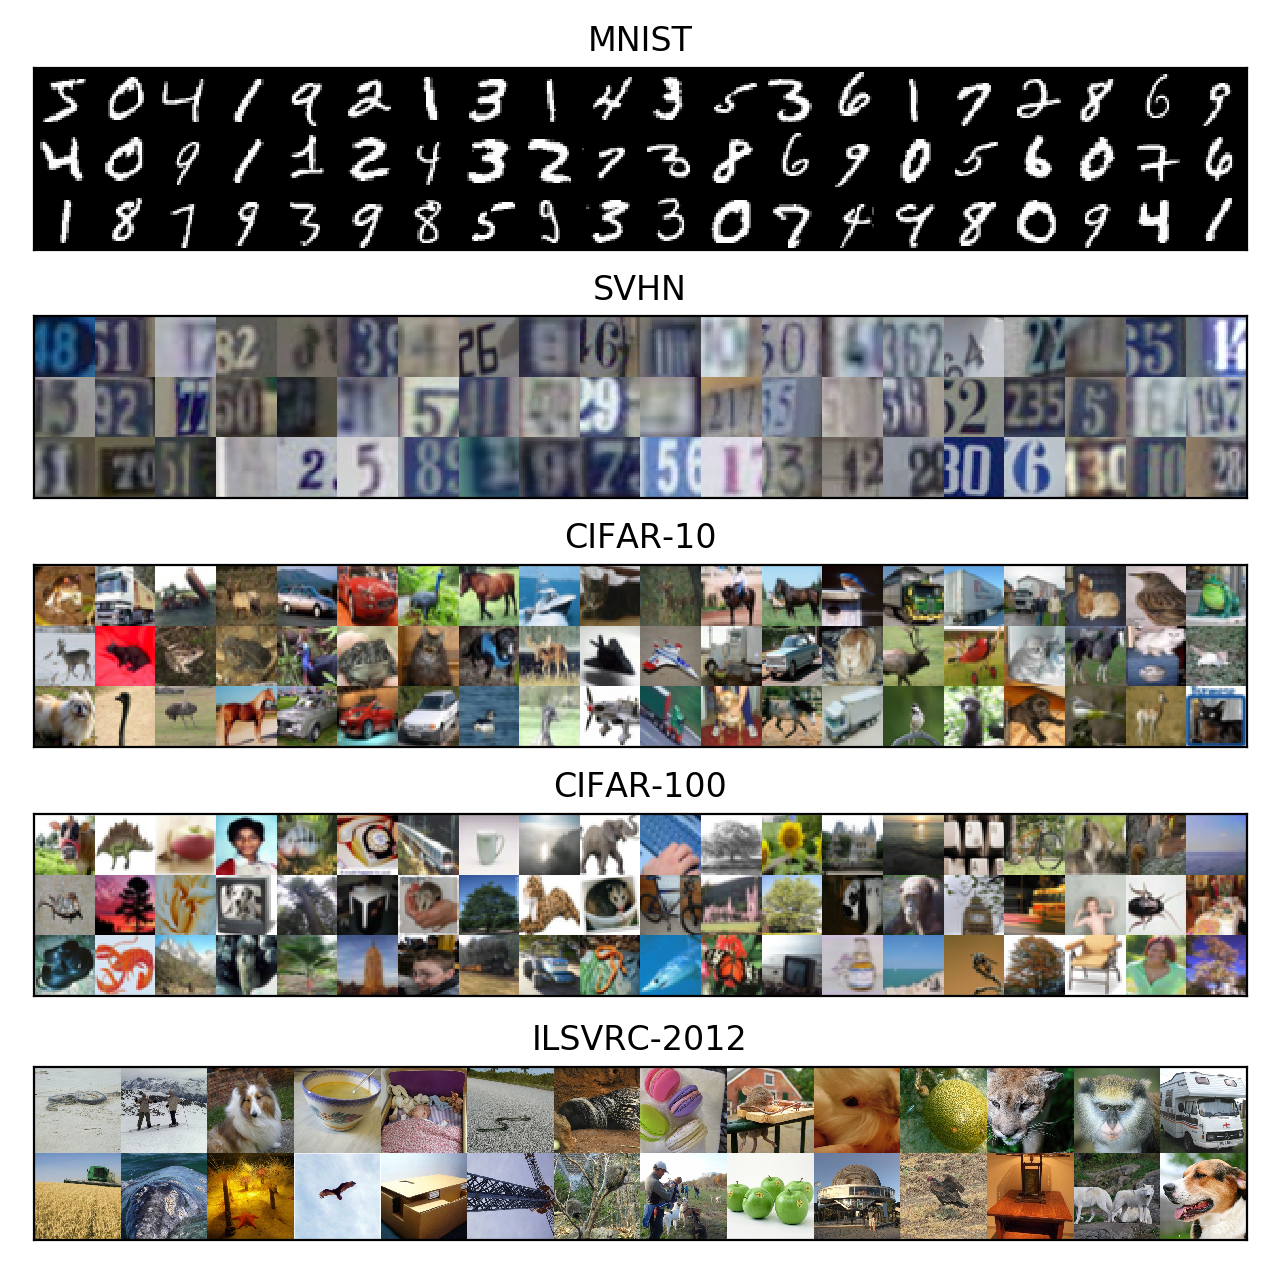
\includegraphics[width=6.35in]{datasets.png}
  \captionb{Example images from datasets used in this thesis.}{}
  \figlabel{datasets}
\end{figure}

The MNIST dataset \parencite{Lecun1998} is a collection of handwritten digits
(taken from US zip codes written on envelopes).
The digits have been heavily preprocessed such that each image
contains exactly one centred digit in high contrast greyscale
(essentially black and white).
Optical classification of handwritten characters is a challenging problem,
and the first true success on this problem by \textcite{Lecun1998}
marked a turning point in machine learning.
While the dataset is no longer challenging for state-of-the-art methods,
it is still commonly used as a first benchmark for novel models and methods.
Its relatively small size (by modern standards)
allows for expedient training even with slower methods
(\eg/ online learning and spike-based methods).

The SVHN dataset \parencite{Netzer2011} is also composed of digits,
taken from images of house numbers on Google Street View.
They show large variation in the styles of digits,
as well as in the backgrounds, lighting, colours, and contrast.
They have been preprocessed such that each image is centred
on a digit (the target digit for classification),
however images often contain whole or partial digits to the sides
(distractor digits).
This makes the dataset considerably harder than MNIST,
but still relatively easy compared to datasets composed of objects.
State-of-the-art algorithms achieve under 2\% error,
which is better than the estimated human error of 2\% \parencite{Netzer2011}.

The CIFAR-10 and CIFAR-100 datasets \parencite{Krizhevsky2009}
consist of small ($32 \times 32$ pixel) images from
10 or 100 different categories, respectively.
All the images are taken from the Tiny Images Dataset \parencite{Torralba2008},
and are in full colour.
Despite being the same size as the SVHN dataset,
these datasets are considerably harder:
Human performance on CIFAR-10 has been estimated at 94\% accuracy \parencite{Karpathy2011},
and state-of-the-art algorithms get around 96\% accuracy \parencite{Springenberg2015,Graham2015}.
CIFAR-100 is even more difficult,
with state-of-the-art accuracy around 75\% \parencite{Graham2014a,Clevert2015a}.
The main reason for the increased difficulty is that the object categories
are simply more diverse,
with members of each category encompassing a wide range of visual features,
and with a larger variety of object poses in each category.
For example, one category in CIFAR-10 is ``dog'';
the dataset includes images of many different breeds of dogs,
with a wide range of appearances,
taken from many different angles.
With CIFAR-100 there is the additional problem that there are more categories,
thus greatly reducing the probability of guessing the correct category by chance.
Furthermore, many of the categories are similar---%
for example ``shrew'' and ``mouse''---%
and it is difficult to consistently differentiate these categories
using small images taken from a variety of angles.

The ILSVRC-2012 dataset
(ImageNet Large Scale Visual Recognition Challenge 2012 dataset, \textcite{Russakovsky2015})
more colloquially known as the ImageNet dataset,
is a dataset of images drawn from the ImageNet database.\footnote{
  \url{http://www.image-net.org/}}
The ImageNet database is a set of medium to high resolution images,
organized into hierarchical categories called synsets (for ``synonym set'').
It contains millions of labelled images.
The ILSVRC-2012 dataset is a subset of these images,
used for the ImageNet Large Scale Visual Recognition Challenge contest in 2012.
This subset has images labelled with 1000 different categories,
predominated by animal species, plants, household objects, vehicles,
and building/room types (both exterior and interior).\footnote{
  To give an illustration of the diversity of the classes,
  here are some examples:
  Great Dane, gazelle, titi monkey, hartebeest, panda, llama,
  forklift, snowplow, fire truck, pool table, throne, seashore, volcano,
  hummingbird, box turtle, mud turtle, guillotine, barometer, stove,
  cannon, car wheel, screw, jellyfish, toaster, waffle iron, vacuum,
  library, planetarium, church, restaurant, butcher shop, sock, CD player, bubble.
  For the building types, the categories vary as to whether the images
  are from inside or outside the building.
  For example, ``library'', ``restaurant'', and ``butcher shop'' all predominantly
  contain images from inside those buildings,
  whereas ``planetarium'' consists of images from outside planetariums;
  ``church'' contains images from both inside and outside churches.}
The images are not all exactly the same size,
and preprocessing often consists of scaling and cropping the images
to be $256 \times 256$ pixels,
though some researchers have experimented with varying sizes \parencite[\eg/][]{Simonyan2015}.
This dataset is considerably harder than the previous ones,
not only because there are many more categories,
but also because images often contain a number of objects,
and it is sometimes a bit ambiguous which object is the ``focus'' of the image
(see \fig{datasets}).

Considering these challenges,
modern machine learning algorithms have performed quite well.
Since there are so many categories, many algorithms have published
both top-5 and top-1 results:
top-5 means that if the actual label for the test image
is in any of the top five categories predicted by the algorithm,
then the image is considered correctly classified;
top-1 means that the top prediction has to match the correct label.
Top-5 classification helps accommodate the fact that there are ambiguous images
with multiple featured objects,
and that there are some categories that appear quite similar
and would be difficult even for a human to distinguish from all angles
(\eg/ some breeds of dogs).
\textcite{Krizhevsky2012} won the inaugural competition in 2012
with a top-5 score of 15.3\%;
since then there have been many significant improvements,
notably \textcite{Simonyan2015} who achieved 6.8\% top-5 error
using multi-crop evaluation (8.0\% using standard single-scale evaluation),
and \textcite{Szegedy2016} who achieved 3.1\% top-5 error
using a combination of four of their Inception models with multi-cropping
(any of the individual models achieves 5\% top-5 error without multi-cropping).


\section{Backpropagation}
\scnlabel{backprop}

The backpropagation (BP) algorithm
(short for ``backwards propagation of gradients'', \aka/ ``backprop'')
is the algorithm chiefly responsible for the recent success of machines
on object recognition tasks.
Though the algorithm was
%% proposed in the 1970's by \textcite{Amani1975} and
brought to wider attention in the 1980's by \textcite{Rumelhart1985},
it was only mildly successful at the time,
largely due to lack of computational resources.
As computers developed,
and some of the finer points of machine learning became better understood,
backpropagation became increasingly useful,
culminating in LeNet \parencite{Lecun1998},
a deep convolutional network that marked the first significant success
on the MNIST handwritten digit dataset,
and a seminal success of neural networks in general.

Since that time, the algorithm has continued to gain traction.
In the 2000's, backpropagation was used to ``fine-tune'' many types of deep networks:
it was used at the end of a training algorithm to make moderate adjustments
to network weights that would provide a significant decrease in error
at the end of a training regime.
Other algorithms were used for ``pretraining'',
that is, determining initial weights that could be moderately successful
at a task and provide a starting point for backpropagation.
One such method was layer-wise pretraining,
where each layer in a deep network was trained as
an autoencoder or restricted Boltzmann machine (RBM),
to be able to represent well the information in the previous layer.
This unsupervised training would initialize the network to a state
where the final hidden layer retained a significant amount of information
about the inputs.
Backpropagation could then be used to train the output classifier,
as well as fine-tune the weights of the previous layers.
It is only more recently, since around 2010,
that backpropagation has been used to train networks from scratch.\footnote{
  There are three main factors that converged to make this possible.
  Increasing computation power---specifically using GPUs---%
  allowed for training larger models on larger datasets in a reasonable
  amount of time.
  Rectified linear units (ReLUs, see \scn{cnn-nonlinearities})
  made training less sensitive to the initial weights,
  since they are scale-invariant and make
  vanishing and exploding gradient problems less likely.
  Convolutional networks, while already used successfully a decade earlier,
  were combined with these methods,
  greatly reducing the number of parameters as compared with
  fully connected methods like RBMs.}
Currently, backpropagation is the main workhorse used for training almost all deep networks.

Backpropagation is a method for determining
the gradients of the network parameters
with regards to an objective function.
It solves what is known as the \emph{spatial credit assignment problem}:
given a particular error at the output of the network,
which hidden units are responsible for that error,
and by extension which parameters should be changed to most quickly
decrease the error?
Put another way, how do we assign credit (or blame)
to the hidden units for their role in the network output?
This was a significant problem for early neural network researchers.

If we have a single-layer linear network,
it is easy to take the derivative of the objective function
with respect to the parameters.
For example, if we have a network $\vect y = \mat W \vect x$,
and objective function $O = \frac{1}{2}\|\vect y - \vect y^*\|_2^2$,
then
\begin{align}
  \diff{O}{\mat W} &= \diff{}{\mat W} \|\mat W \vect x - \vect y^*\|_2^2 \nonumber\\
                   &= (\mat W \vect x - \vect y^*) \diff{\mat W \vect x}{\mat W} \nonumber\\
                   &= (\mat W \vect x - \vect y^*) \vect x^T \text{ .}
\end{align}
This becomes less straightforward
when we have layers of nonlinear hidden neurons.
If we have a network $\vect y = \mat W f(\mat V \vect x)$
(where $f(\cdot)$ is an elementwise nonlinearity),
how do we determine $\diff{O}{\mat V}$?

This is the problem that the backpropagation algorithm solves.
It does this by successively applying the chain rule of calculus,
to pass error information from the output of the network
backwards to previous hidden layers of the network.
The algorithm begins by first computing the activations
of all neurons in the network for one or more inputs
(this is known as the forward pass).
The algorithm then successively computes the derivatives
of all parameters in the network,
starting with the parameters of the final hidden layer
(right before the output layer),
and working backwards through the network.
This is known as the backwards pass.

Assume we have two successive hidden layers in a neural network,
$\vect h^{n-1}$ and $\vect h^n$,
connected with a full set of weights and a nonlinearity such that
\begin{align}
  h_j^n &= f\left(a_j^n\right) \nonumber\\
        &= f\left(\sum_i W_{ij}^n h_i^{n-1} + b_j^n\right)
\end{align}
where $W_{ij}^n$ is the weight connecting hidden unit $h_i^{n-1}$ and $h_j^n$,
$b_j^n$ is the bias for hidden unit $h_j^n$,
and $a_j^n \equiv \sum_i W_{ij}^n h_i^{n-1} + b_j^n$ is the input activity
to the nonlinearity $f(\cdot)$ for $h_j^n$.
For simplicity, I assume the same nonlinearity for all hidden neurons,
but it is easy to relax this assumption.

We can now take the derivative across this hidden layer pair.
Let $e_i^n \equiv \diff{O}{h_i^n}$, that is $\vect e^n$
is the error gradient of the $n^\text{th}$ hidden layer.
Using the chain rule of calculus,
we can find the error of the previous layer $\vect e^{n-1}$
in terms of the error of the current layer $\vect e^n$:
\begin{align}
  e_i^{n-1} &= \sum_j \diff{O}{h_j^n} \diff{h_j^n}{h_i^{n-1}} \nonumber\\
           &= \sum_j e_j^n \diff{f(a_j^n)}{a_j^n} \diff{a_j^n}{h_i^{n-1}} \nonumber\\
           &= \sum_j e_j^n f'(a_j^n) W_{ij}^n \text{ .}
\end{align}
This equation can be used to recursively calculate the error at each layer,
starting from the error at the top layer
(which is determined by differentiating the objective function
with respect to the network outputs).
From this error, we can calculate the derivatives of the objective function
with respect to each of the parameters:
\begin{align}
  \diff{O}{W_{ij}^n} &= \diff{O}{h_j^n} \diff{h_j^n}{a_j^n} \diff{a_j^n}{W_{ij}^n} \nonumber\\
                    &= e_j^n \diff{f(a_j^n)}{a_j^n} \diff{a_j^n}{W_{ij}^n} \nonumber\\
                    &= e_j^n f'(a_j^n) h_i^{n-1} \\
  \diff{O}{b_j^n} &= \diff{O}{h_j^n} \diff{h_j^n}{a_j^n} \diff{a_j^n}{b_j^n} \nonumber\\
                  &= e_j^n \diff{f(a_j^n)}{a_j^n} \diff{a_j^n}{b_j^n} \nonumber\\
                  &= e_j^n f'(a_j^n) \text{ .}
\end{align}
These derivatives can then be used to update the parameters,
using an optimization method like the one discussed below (SGD, \scn{sgd}).

The above derivation shows how to differentiate an objective function
based on one example;
real objective functions often sum across many examples.
Since differentiation is a linear operator,
the derivative of a cost function that sums across many examples
is equal to the sum of the derivatives for each of the individual examples.
Thus, we can compute the derivatives for each example separately,
and sum them together at the end.


\section{Stochastic gradient descent (SGD)}
\scnlabel{sgd}

Backpropagation provides a method to take the first-order derivative (gradient)
of the cost function with respect to the network parameters.
It does not define how to use that gradient to minimize the cost;
there are a number of potential methods to do this.

The most basic method is adjusting the parameters
in the direction of the negative gradient;\footnote{
  The gradient points in the direction in which the cost increases most quickly.
  Thus to decrease the cost most quickly,
  we move in the direction of the negative gradient.}
this is known as \emph{gradient descent}.
By definition, only an infinitesimally small step in this direction
will decrease the cost,
since the function may only decrease for an arbitrarily short distance
before starting to increase again.
In practice, however, we must take a significant step in the gradient direction.
The step size is modulated by the \emph{learning rate},
which is multiplied by the gradient to determine the step.
There is a tradeoff between a large learning rate,
which will allow us to converge more quickly for smooth (well-conditioned) objectives,
and a small learning rate,
which will ensure stability (convergence) on more ill-conditioned problems.
As long as the learning rate is small enough,
then gradient descent can converge for any problem.

When performing gradient descent,
we compute the gradient across all training examples (called the batch)
for each parameter update;
this is computationally expensive.
%% According to the theory of gradient descent,
%% To ensure that the cost for the whole training set decreases at each time step,
%% we must use the whole training when estimating the gradient,
%% otherwise our parameter update may decrease the cost for some examples
%% but increase it for others.
%% But computing the gradient using the whole training set is costly.
Stochastic gradient descent (SGD) solves this problem by simply
using part of the training set to estimate the gradient at each iteration,
accepting the risk that this may sometimes increase the overall cost.
At each iteration, we are computing a noisy or stochastic estimate of the gradient.
As long as the corresponding parameter updates are beneficial on average,
the overall cost should decrease.
The examples used to estimate the gradient are called the mini-batch.

The size of each mini-batch is an important parameter in SGD.
Having more examples in the mini-batch means that we get
a better estimate of the gradient,
but it also means more computation per mini-batch.
Choosing the mini-batch size is a tradeoff between these two criteria;
in practice, typical sizes are around 20 to 100 examples.

SGD is a popular method because it is relatively simple to implement,
and can work well on a wide variety of problems.
Most neural networks are sufficiently large and complicated that
second-order methods
(which require the explicit computation of second-order derivatives, called the Hessian)
are not tractable.
Even methods that estimate the second-order derivatives---%
such as L-BFGS \parencite{Liu1989}---%
cannot deal with the size of modern neural networks,
since the number of elements in the Hessian equals
the number possible of pairs of parameters in the model.
Hessian-free optimization \parencite{Martens2010} is able to avoid this problem,
and has been applied to neural networks,
most commonly recurrent neural networks for which
the vanishing and exploding gradient problems (\scn{init})
are particularly potent.


\subsection{Extensions}

Momentum \parencite{Polyak1964} is a simple addition to SGD updates;
it is inspired and named because of its similarity to physical inertial momentum.
Given the current parameters $\theta_t$
and their corresponding gradient on the current mini-batch $\nabla f(\theta_t)$,
standard SGD computes the new parameters $\theta_{t+1}$ as
\begin{align}
  \theta_{t+1} = \theta_t - \alpha \nabla f(\theta_t) \text{ .}
\end{align}
To compute the same update with momentum $\mu \in [0, 1]$,
we introduce the intermediate variable $v_t$
that accumulates a running total of past gradients:
\begin{align}
  v_{t+1} &= \mu v_t - \alpha \nabla f(\theta_t) \\
  \theta_{t+1} &= \theta_t + v_{t+1} \text{ .}
\end{align}
This is quite similar to a running estimate of
the first moment (\ie/ mean) of the gradient,
and has a similar effect to averaging:
it smooths over high-frequency fluctuations in the gradient
due to the imprecise nature of computing it on a small set of samples,
and focuses movement to address the persistent, low-frequency errors.
Another way to view this is if you have a long narrow valley
in the cost function parameter space,
momentum helps to reduce the movement side-to-side across the valley
(the high-frequency errors)
and focuses movement down the valley (the low-frequency errors).
This can help the optimization to move more quickly through
flat regions in the optimization space (\ie/ saddle-points),
which are quite prevalent in the high-dimensional optimization problems
faced by ANNs \parencite{Dauphin2014}.

Nesterov momentum \parencite{Sutskever2013} is an important variant.
Rather than computing the gradient on the parameters,
and using this to update $v_t$ which then updates the parameters,
Nesterov momentum applies the momentum update to the parameters first,
such that the gradient is computed on the parameters with momentum:
\begin{align}
  v_{t+1} &= \mu v_t - \alpha \nabla f(\theta_t + \mu v_t) \\
  \theta_{t+1} &= \theta_t + v_{t+1} \text{ .}
\end{align}
This results in a more accurate gradient estimate,
since it is computed at the location (in parameter space) where we apply it.

There are a number of other extensions to SGD,
many of which are concerned with automatically adjusting learning rates
for individual parameters.
To do this, these methods divide by some measure
of the average gradient magnitude over time
(\eg/ a running average of the RMS value or the second moment).
This helps improve convergence when parameters are on different scales
(for example, if different layers have different magnitude weights),
as well as other situations when derivatives for different parameters
have consistently different magnitudes.
\textcite{Ruder2016} provides a good overview of the most common methods,
and compares their performance on a few demonstration problems.
Adam \parencite{Kingma2015} is one of the best-performing.
It keeps running estimates of both
the first moment of the gradient (just as momentum does)
and the second moment (which is a measure of the gradient magnitude for each parameter).
Parameter updates are proportional to the first moment
divided by the square root of the second moment.
Nadam \parencite{Dozat2016} adapts Adam to use Nesterov momentum
instead of classical momentum.


\subsection{Gradients and initialization}
\scnlabel{init}

Two common problems faced during ANN optimization
are what are known as the vanishing and exploding gradient problems.
These problems become more prevalent as networks get deeper
(or recurrent, since recurrent networks are often optimized like deep networks
with tied parameters between layers).
The vanishing gradient problem occurs when the magnitude of the gradient
becomes near zero, and the optimization becomes very slow.
This indicates a saddle-point in the parameter space,
a prevalent problem when optimizing ANNs \parencite{Dauphin2014}.
If the gradient of one layer prematurely approaches zero,
for example if almost all neurons in a layer have become silent,
then the gradients for other layers will quickly approach zero as well,
because the cost can only be reduced so much when one layer is not functioning.

The exploding gradient problem occurs when gradients quickly become too large.
This is typically caused by instability in the SGD algorithm
when the learning rate is too large.
Once the algorithm becomes even slightly unstable,
it is difficult for it to regain stability.
For example, a high learning rate can make the algorithm
step well past the minimum in the gradient direction to an area of higher cost;
this higher cost results in the next gradient---%
and thus the next step---being too large,
resulting in an even higher cost, and the algorithm spirals out of control.

The vanishing and exploding gradient problems can stem from
the initialization of the network.
Layers with parameters that are too large or too small can cause problems
(especially with sigmoid nonlinearities, since these have zero derivative
for both large negative and positive values).
%% as well as different parameter magnitudes between layers.
A number of initialization schemes have been developed to help counteract these problems.
The idea behind these methods is that the variance information passing both
forwards (activations) and backwards (derivatives) through the network
should remain the same.
\textcite{Glorot2010} and \textcite{He2015} both present formulae
for choosing initial Gaussian weight magnitudes,
based on the assumptions that neurons have linear or rectified-linear activation functions,
respectively.
\textcite{Mishkin2016} proposes a more general method
that iteratively adjusts initial weight magnitudes
based on a sample of the training data;
this method can work for networks with arbitrary nonlinearities,
as well as networks that include max-pooling and contrast normalization layers,
among others.


\section{Convolutional neural networks (CNNs)}
\scnlabel{cnns}

Convolutional neural networks (CNNs) have become the mainstay
of neural networks for object recognition.
Unlike many other types of networks,
CNNs have shown that they are able to scale to large datasets containing
many images with many pixels each.
This is because CNNs use a convolution operation,
which greatly reduces the number of parameters used by the model.
Fewer parameters means less training time and fewer labelled examples
are needed to adjust the parameters,
making much larger datasets tractable.
This idea takes inspiration from neuroscience:
primary visual cortex (V1) neurons have similar tunings (filters)
that are repeated across the whole visual space.
In this section, I describe the main components of CNNs.
%% Credited by some? as the key innovation in machine learning in the past decades


\subsection{Convolution operation}
\scnlabel{convolution}

%% What is convolution?
The basic idea of convolution is used heavily in engineering,
particularly signal processing,
where a filter (specifically its impulse response) is convolved with a signal
to produce a filtered version of the signal.
In the case of CNNs for object recognition in static images,
convolution almost always refers to a \dd/ convolution
across the x- and y-dimensions of the image.\footnote{
  CNNs for processing video sometimes use \ddd/ convolutions,
  with the third dimension as time.
  CNNs for processing time signals (\eg/ auditory waveforms) can use
  \mbox{1-D} filters.
  We will only treat the \dd/ case here.}
In basic image processing, an example of a convolution would be convolving
a \dd/ Gaussian kernel with an image,
to produce a smoothed version of the image.
Edge detection can be performed by convolving an edge detecting filter
(\eg/ the Sobel operator) with an image.

The \dd/ image convolution operation describes how
a set (\aka/ bank) of filters (\aka/ kernels) acts on a multi-channel image,
to produce another multi-channel image.
The term ``image'' is used loosely, here,
since the number of channels $n_c$ may be large (greater than three),
and thus the image may not be visualizable in a normal way.
Each filter has the same number of channels $n_c$ as the input image,
and convolving it with the input image produces one channel of the output image.
Thus, the number of channels in the output image
is the same as the number of filters $n_f$.

Let $X(i,j,c)$ be an image where $i \in [0, n_i)$ and $j \in [0, n_j)$
index the vertical and horizontal positions, respectively,
and $c \in [0, n_c)$ indexes the channel (all indices are integers).
%% Therefore, we have an $n_i \times n_j$ image with $n_c$ channels.
We filter the image using a filter bank $F(p,q,c,k)$,
where $u \in [0, s_i)$ and $v \in [0, s_j)$ index
the vertical and horizontal positions in the filter, respectively,
$c$ again indexes the channel,
and $k \in [0, n_f)$ indexes the filter itself.
Therefore, we have a bank of $n_f$ filters, where each filter is
$s_i \times s_j$ pixels with $n_c$ channels.
The convolution is given by
\begin{align}
  Y(i,j,k) = \sum_{u=0}^{s_i} \sum_{v=0}^{s_j} \sum_{c=0}^{n_c}
      X(i+u, j+v, c) F(s_i-u-1, s_j-v-1, c, k).
  \eqnlabel{convolution}
\end{align}
For some $i+u$ and $j+v$, these indices will be outside the domain of the image,
in which case the value of the image is assumed to be zero.
Note that the indices for the filter are ``flipped'' versions of
the indices $u$ and $v$.
This is because convolution flips the filter before applying it
(\cf/ correlation, which is the same operation but without a flip).
That said, some deep learning libraries do not implement the flip,
because this aspect of convolution typically has no effect on learning algorithms.

For more explicit control over the application of the filters to the image,
many deep learning libraries implement strides and padding.
The \emph{stride} of a convolution refers to the spacing at which the filter is applied.
For example, a stride of three means the filter is applied every third pixel
(instead of every pixel as in \eqn{convolution}).
The \emph{padding} of a convolution describes how many rows and columns of zeros
are added to the outside of the image before applying the filter.
(Often, these zeros are not explicitly added,
but rather dealt with implicitly.)
Let $q_i$ and $q_j$ denote the strides
in the vertical and horizontal directions, respectively,
and $p_i$ and $p_j$ denote the padding along either side,
again in the vertical and horizontal directions, respectively.
The strided, padded convolution is given by
\begin{align}
  Y(i,j,k) = \sum_{u=0}^{s_i} \sum_{v=0}^{s_j} \sum_{c=0}^{n_c}
      X(q_i i+u-p_i, q_j j+v-p_j, c) F(s_i-u-1, s_j-v-1, c, k) \text{ .}
  \eqnlabel{convstrided}
\end{align}
Again, the image $X$ is assumed to be zero for any indices outside its domain.
This provides the implicit padding.
We also need to address the allowable range of values for $i$ and $j$.
Often, for padded convolutions, only $i$ and $j$ such that the filter
falls entirely in the padded image are used.
This is referred to as a ``valid'' convolution.\footnote{
  When not using padding,
  the term ``valid'' refers to convolutions in which all filter positions
  fall entirely in the image proper.}
For \eqn{convstrided} to be a valid convolution vertically,
we need $q_i (m_i - 1) - p_i + s_i \le n_i + p_i$
where $m_i$ is the height of the output image (\ie/ $i \in [0, m_i)$).
Solving for $m_i$ we find that
\begin{align}
  m_i &= 1 + \left\lfloor \frac{n_i + 2p_i - s_i}{q_i} \right\rfloor
\end{align}
where $\lfloor\cdot\rfloor$ is the floor operation (\ie/ round down to the nearest integer).
Substituting the index $j$ for $i$ will give a similar formula
for the horizontal direction.
One downside to this formulation is that depending on the strides and padding used,
some pixels in the input image may not be used in computing the output image.
To remedy this, some libraries (\eg/ \texttt{cuda-convnet2})
take the ceiling $\lceil\cdot\rceil$ instead of the floor,
ensuring that all input pixels are used.
If the stride divides evenly into the image size plus padding minus filter size,
then no rounding is required and both methods are the same.


\subsection{Convolutional layer}

The core element of CNNs is the \emph{convolutional layer}.
A convolutional layer performs a linear convolution operation (\eqn{convstrided}).
It is typically followed by a neural nonlinearity.
Compared to a fully connected layer,
a convolutional layer has two main differences:
1) the connectivity is local; and
2) the weights are shared between units.

Local connectivity means that each unit only connects to a subset of the input units
in a particular region of the input.
This region is called the receptive field (RF),
in analogy to the concept in neuroscience.
With CNNs, this is almost always a rectangular region,
and most often a square region.
For example, one output unit may take input from a $9 \times 9$ region of the
input image in the top left corner,
and another from a similarly sized region in the bottom right.
One advantage of local filters are that they greatly reduce
the number of parameters in the model.
If we assume a realistic image size such as $256 \times 256$,
even using a relatively large RF size of $32 \times 32$ yields
$\sim 1.5\%$ the parameters of a fully connected model,
and using $11 \times 11$ RFs yields less than $0.2\%$ as many parameters.
This helps reduce overfitting.
An additional advantage is that since output units are receiving input from
different parts of the image,
their activities are less correlated.
Typically, correlation between units is undesirable,
since it reduces the amount of unique information contained in each signal.

Shared weights means that each unit applies the same weights to its
designated RF.
As described in \scn{convolution},
this can be thought of as taking a filter and passing it across the image,
evaluating the response at each filter position.
For this weight sharing to work,
all output units must have RFs that are the same size.
Furthermore, it is common practice to have the RFs of
output units be spaced at regular intervals
(called the stride, see \scn{convolution}).
While this regularity is not strictly necessary,
it makes the implementation easier.
The advantage of shared weights is that it further reduces the number of parameters.
It allows the same parameters to be tuned using all parts of the image simultaneously,
thus expediting the learning process.
It is also an example of a brain-inspired architecture,
since the tuning of neurons in early visual cortex (V1)
has been found to have similar statistics across the visual field.
It should be noted, however, that this does rely on the assumption
that image statistics are similar across the whole image.
Otherwise, the same filter will not be ideal for all areas of the image.
\textcite{Krizhevsky2012} found that the statistics at the edges of the image
are different than in the centre (due to the padding used for convolution),
and they used separate filters for dealing with the image edges.


\subsection{Nonlinearities}
\scnlabel{cnn-nonlinearities}

The nonlinearity is essential to any deep network,
since it provides the power to go beyond the capabilities of a a linear perceptron
and compute nonlinear functions of the inputs.

Typically, a layer of nonlinearities will always follow some form of weight layer
(\eg/ a convolutional layer or a fully connected layer).
These layers rarely appear separately for two reasons:
First, having two weight layers without some nonlinearity in between is redundant,
since weight layers are linear,
and two linear operations in a row cannot compute any functions that a single
linear operation cannot compute.\footnote{
  This is not strictly true for a CNN,
  since convolutional layers have limited receptive fields,
  thus chaining them increases the effective receptive field.}
In fact, chaining weight layers without a nonlinearity in between
can be problematic for the optimization,
since it overparametrizes the system
(\ie/ there are many combinations of parameters that produce the same results).
Second, each nonlinearity is preceded by a weight (parametrized) layer
because this gives the optimizer control over how that layer is used.
Having two nonlinearity layers separated by a non-parametrized layer
(\eg/ a pooling layer) would force the system to use that combination
of three layers without having any control over what (complex) function
they are computing.
Having nonlinearity layers always preceded by weight layers
gives the system much more flexibility.

In a nonlinearity layer,
the nonlinearity is almost always element-wise:
it is defined by a function with scalar input and output (the nonlinearity),
which is applied independently to each element of the input image.
The question, then, is what nonlinearity to use.

Classical neural networks often used sigmoid nonlinearities.
These nonlinearities, most commonly either the hyperbolic tangent
or logistic sigmoid function,
have an ``S'' shape.
They were often deemed desirable because
they are what are called \emph{compressive} nonlinearities:
their domain is the whole set of reals,
and they compress this space into values in a limited range
(typically either $(-1, 1)$ or $(0, 1)$).
They are also easily differentiable,
making them suitable for use with algorithms like backpropagation,
and vaguely resemble the rate response functions of cortical neurons.

Currently, most CNNs use rectified linear units (ReLUs),
given by $f(x) = \max(x, 0)$ \parencite{Nair2010}.
These units output zero for all inputs below zero,
and are linear (specifically, the identity function) for all inputs above zero.
This function is desirable because of its derivative,
which is the step (\aka/ Heaviside) function
(zero for inputs below zero, one for inputs above zero).
The advantage of this derivative is that it
maintains the magnitude of the derivative from previous layers
for all units that are active.
This helps avoid both the vanishing and exploding gradient problems.
Another way to think of this is we have a linear optimization problem
among the units that are active,
and ignore the units that are inactive.
Since linear optimization problems are typically better behaved than nonlinear ones,
this makes the optimization easier.

These benefits also relate to the fact that ReLUs are scale-invariant:
\begin{align}
  f(\alpha x) &= \alpha f(x) \nonumber\\
  \max(\alpha x, 0) &= \alpha \max(x, 0) \text{ ,}
\end{align}
where $\alpha$ is a scalar.
This means that scaling the input weights of a ReLU layer by a constant
scales the outputs of the layer by that same constant,
which makes ReLU layers much easier to initialize.
With sigmoid layers, if the input weights are too large or too small,
all outputs will be near one or zero respectively,
which in both cases lead to a derivative of zero
and loss of information through the network.
With ReLUs, on the other hand, the relative spacing between inputs
is preserved for inputs above zero.

The maxout nonlinearity was introduced by \textcite{Goodfellow2013}
as a natural companion to the dropout regularization technique (\scn{dropout}).
As discussed above, nonlinearities typically follow weight layers.
The previous nonlinearities presented here can each be thought of
as having a weight vector that is multiplied by the inputs to produce a scalar value,
which is then passed through the nonlinearity to produce the output
(when we discuss a whole layer, then we have a weight \emph{matrix},
which is the collection of the vectors for the individual hidden units).
With the maxout nonlinearity, each hidden unit has multiple vectors (a matrix),
which when multiplied by the inputs generates a vector input to the nonlinearity.
The maxout nonlinearity then returns the maximum element of this vector.\footnote{
  This procedure is equivalent to using cross-channel max-pooling
  across a number of ReLU units,
  but without including zero in the max.
  \textcite{Goodfellow2013} finds that this is a significant difference,
  and that including zero is detrimental to performance compared to maxout.}
The resulting effect is that the maxout nonlinearity can implement
a wide range of simpler nonlinearities (including ReLU, absolute value, and quadratic)
depending on the input weights.
This gives maxout networks choice over what nonlinearities to use, and where.
For unregularized networks, this could easily provide too much power,
and result in overfitting and poor generalization.
When combined with dropout, maxout works quite well,
performing better than standard (ReLU and tanh) nonlinearities,
particularly for deeper networks.


\subsection{Pooling layer}

Pooling layers combine information across space in a convolutional network.
They take an input image, and output an image with a reduced width and height,
but leave the number of channels unchanged.
Pooling across channels (feature maps) is also possible,
but is not common, and is not addressed here.

The motivation behind pooling is to add \emph{translation invariance}
to networks.
Inspiration comes from simple and complex cells in the brain.
When shown a sinusoidal grating,
simple cells are sensitive to the phase of the grating,
whereas complex cells are not.
Thus, complex cells are invariant to translations of the grating.
Since CNNs learn features that are computed at various translations across
the image,
they provide an opportunity for building in translation invariance
that is not available with fully or locally connected networks.
By pooling across the output of the same feature,
at adjacent locations,
the output of the pooling layer should be (somewhat) invariant
to translations of that feature.

For a general pooling layer,
each output value is a function
on some neighbourhood of points in the input image.
That is, we can think of each output pixel as having a target point
in the input image,
and the output value is a function on all points close to that target point,
called the pooling region.
To retain all data,
the pooling regions should completely cover the input image space.
There are two common types of pooling:
non-overlapping pooling, in which pooling regions tile the input space,
but no two overlap;
and overlapping pooling, where adjacent pooling regions overlap.
As with the receptive fields in a convolutional layer,
we can fully define the size and spacing of pooling regions
with size $s$ and stride $q$ hyperparameters, in both directions.
For non-overlapping pooling, size $s = 2$ and stride $q = 2$ is by far
the most common configuration.
For overlapping pooling, size $s = 3$ and stride $q = 2$ is typical.
Larger pooling regions are theoretically possible,
but in practice they are rarely used,
because they result in more information being lost
and thus poorer performance.
% ^ http://cs231n.github.io/convolutional-networks/#pool

The most common pooling operation is max-pooling.
It computes the maximum value across the pooling region for each output pixel:
\begin{align}
  Y(i,j,c) = \max_{u,v=0}^{s_i,s_j} X(i q_i + u, j q_j + v, c)
\end{align}
where $s_i$ and $s_j$ are the height and width of the pooling region,
and $q_i$ and $q_j$ are the strides in the vertical and horizontal directions,
respectively.
This provides good translation invariance
because if a feature has maximum value at a particular point in the image,
then shifting the image such that that maximum remains in the same pooling region
will result in the same output value for that pooling region.

To use a max-pooling layer in a network trained by a gradient-based method,
we must be able to compute the gradient of the inputs with respect to the cost.
If $X(u,v,c)$ is in the pooling region of $Y(i,j,c)$, then:
\begin{align}
  \diff{C}{X(u,v,c)} = \begin{cases}
    \diff{C}{Y(i,j,c)} & \text{if } X(u,v,c) == Y(i,j,c) \\
    0 & \text{otherwise}
  \end{cases}.
\end{align}
That is, if $X(u,v,c)$ is the maximum value in its pooling region,
then its gradient is one times the gradient of its output
(\ie/ the gradient passes through),
otherwise the gradient is zero.
This makes sense, since if $X(u,v,c)$ is the maximum value in its pooling region,
then only changes to it will change the output value
(unless of course it changes enough that it is no longer the maximum value).
When we have overlapping pooling, such that $X(u,v,c)$ falls in multiple pooling regions,
then its gradient is the sum of the gradients computed for each constituent pooling region.

An alternative pooling operation is average-pooling.
It computes the average value across the pooling region for each output pixel:
\begin{align}
  Y(i,j,c) = \frac{1}{s_i s_j} \sum_{u=0}^{s_i} \sum_{v=0}^{s_j} X(q_i i + u, q_j j + v,c)
\end{align}
where again $s_i$ and $s_j$ are the height and width of the pooling region,
and $q_i$ and $q_j$ are the strides in the vertical and horizontal directions,
respectively.
Computing the gradient straightforward, since it is a linear operator:
the gradient $dC / dX(u,v,c)$ is simply the sum of all gradients $dC / dY(i,j,c)$
for which $X(u,v,c)$ is in the pooling region of $Y(i,j,c)$,
scaled by $1 / (s_i s_j)$.
This pooling method was used in many earlier CNNs \parencite[\eg/][]{Lecun1998}.
In standard CNNs, it has largely been replaced by max-pooling,
which seems to perform better for most image recognition tasks.
It is still commonly used in spiking neural networks \parencite[\eg/][]{Diehl2015},
because it is much easier to implement in spiking neurons.


\subsection{Local response normalization layer}

CNNs often include some sort of \emph{local response normalization},
referring to normalizing the output of a layer in a local (rather than global) manner.
The core idea is that for each pixel in the layer,
we compute a normalization factor based on the responses of nearby (local) pixels,
and use this factor to normalize that pixel.
Nearby pixels are usually defined as either being of the same channel
and nearby spatially,
or from the same spatial location but from different feature channels,
or both.
%% Pixels can be nearby in image space, , or both.
%% Responses can be normalized across space,
%% across feature maps (channels), or both.
%% There are two main ways of normalizing responses:
%% normalizing across space,
%% and normalizing across feature maps (channels).
There are also two methods of applying the normalization factor:
either by subtracting it from the input value (subtractive normalization),
or by dividing the input value by it (divisive normalization).

\textcite{Jarrett2009} helped popularize the idea of local response normalization.
They used a combination of subtractive normalization and divisive normalization
across both space and feature maps:
\begin{align}
  X'(i,j,c) &= X(i,j,c) - \sum_{pqr} w_{pq} X(p,q,r) \\
  \sigma_{ij} &= \left(\sum_{pqr} w_{pq} X'(p,q,r)^2\right)^{1/2} \\
  Y(i,j,c) &= X'(i,j,c) / \max\left(c, \sigma_{ij}\right)
\end{align}
where $c$ is the mean $\sigma_{ij}$ across all images and locations.
What makes this computation local is that
$w_{pq}$ is a Gaussian weighting function
centred around $(i,j)$ for the output pixel being computed.
Therefore, both the subtractive and divisive normalization
only normalize over local regions.
They termed this method ``local contrast normalization''.

\textcite{Krizhevsky2012} used only a divisive normalization across the
$N$ feature maps of the layer:
\begin{align}
  Y(i,j,c) = X(i,j,c) / \left(\gamma + \alpha\sum_{k=\max(0,c-s/2)}^{\min{N-1,c+s/2}}
    X(i,j,k)^2 \right)^\beta
  \eqnlabel{kriznorm}
\end{align}
At pixel $(i, j)$, feature map $c$ is normalized by the values of
adjacent feature maps, within a window of width $s$.
Rather than using a standard Euclidean norm,
\eqn{kriznorm} uses a more general norm.
They chose the hyperparameters using cross-validation:
$n = 5$, $\gamma = 2$, $\alpha = 10^{-4}$, and $\beta = 0.75$.
In their code, they refer to this as cross-map response normalization.


\subsection{Dropout layer}
\scnlabel{dropout}

Dropout \parencite{Hinton2012} is a regularization technique
designed to prevent overfitting in ANNs.
By randomly silencing some percentage (\eg/ 50\%) of neurons in a layer
for each stimulus presentation,
one can prevent networks from learning correlated features that are only useful together,
and instead learn features that independently contribute to the classification \parencite{Hinton2012}.
These simpler independent features are less likely to
fit spurious correlations in the data
than complex co-dependent combinations of features,
thus reducing the chances of overfitting.
When the trained network is run on testing images,
all hidden neurons are used (no silencing),
with their activities scaled such that the collective output
of the hidden neurons is the same magnitude as during training.

Theoretically, dropout approximates averaging over many simpler models,
each of which share model parameters \parencite{Baldi2013,Warde-Farley2013}.
Averaging across many separately-trained models
has yielded some of the best results on datasets like MNIST \parencite[\eg/][]{Ciresan2012}.
Being able to harness some of this generalization ability
without the need to explicitly train many networks
(which is time consuming for both training and testing)
makes dropout a powerful technique.
Additionally, when looking at dropout in the context of averaging many simple models,
dropout shares weights between these theoretical models,
while traditional multi-model techniques do not.
\textcite{Warde-Farley2013} find that this gives dropout an advantage
over traditional methods, specifically bagging.

% ubiquity of dropout in modern networks
Dropout has become a very common tool for regularizing deep networks.
The fact that it can be applied to many architectures---
including convolutional, locally connected and fully connected layers---%
makes it a straightforward addition to most networks.
The original dropout paper by \textcite{Hinton2012}
reports significant gains across many different datasets.
\textcite{Srivastava2014} demonstrate that convolutional layers
also benefit from dropout,
which they speculate is because it provides noisy inputs to subsequent layers
thus preventing them from overfitting.


%% \section{Optimizing deep networks}
%% % Where to put this section? It will have to do with optimizing for softlif,
%% % so maybe somewhere related to that

%% % Dead layers
%% One problem that can occur early on during optimization is
%% when no information propagates through the network,
%% and the optimizer decides to either pick output classes randomly
%% or consistently pick one class,
%% both resulting in chance accuracy.
%% In trying to get information from the network input to the network output,
%% the optimizer often ends up driving the activities of one layer to zero
%% (typically the penultimate layer,
%% the layer right before the softmax classifier).
%% % NOTE: once the loss has settled and the layer is actually dead,
%% % the network seems to return the same class for all inputs.

%% While equivalent in terms of accuracy,
%% the minima of consistently picking one class results in a lower loss
%% than randomly picking a class.
%% This is because if the network consistently picks a class,
%% it can say definitel
%% % NOTE: I think they result in different losses, but which way is which?
%% %  Nope, they can be the same or different in terms of loss.
%% %  If one class is slightly higher than the others (\eg/ 0.32, 0.29, 0.29)
%% %  then it will be low loss, whereas if one is very big it will be high

%% This ``dead layer'' problem corresponds to
%% a local minimum in the solution space,
%% where th

%% It can occur for a number of reasons:
%% The initial learning rate is too large,
%% the learning rate is too small,
%% or the layers have not been properly initialized.

%% % http://sebastianruder.com/optimizing-gradient-descent/index.html
%% %  Dauphin et al. suggest that saddle points are actually the culprit, not local minima

%% % ReLUs are scale-free (linear, assuming no offset)
%% % SoftLIF (and others like sigmoid, softplus) are not, so scaling matters more
%% % To help, initialize layers and use optimizer that adjusts LR per layer

%% % Importance of initialization

%%  LocalWords:  compneuro nef Kandel BlausenNeuron Polsky Burnstock
%%  LocalWords:  Goodale Felleman AIT IP RGC Nassi RGCs LGN Vigeland
%%  LocalWords:  Adelson Markram lifrate lif Lillicrap Guergiuev VC
%%  LocalWords:  Lapicque ifdiff lifdifffull lifdiff lifvoltage Spaun
%%  LocalWords:  Mainen Gerstner ji dec GPUs Furber TrueNorth Merolla
%%  LocalWords:  NeuroGrid Mnih Karpathy Xu lrrrrl Lecun Netzer titi
%%  LocalWords:  Krizhevsky Torralba Springenberg Clevert Russakovsky
%%  LocalWords:  synsets hartebeest Simonyan Szegedy Rumelhart Papert
%%  LocalWords:  ij th sgd BFGS Liu init Polyak Sutskever Kingma cnns
%%  LocalWords:  Nadam Dozat Glorot Mishkin convstrided cuda convnet
%%  LocalWords:  maxout Goodfellow dC dX dY Diehl pqr pq kriznorm
%%  LocalWords:  Baldi Warde Ciresan Srivastava Sussman backprop

\chapter{Fixed-Encoding Networks}
\chplabel{nef}

\newcommand{\Dec}{\Omega}
\newcommand{\dec}{\vect \omega}

%% The first type of deep network we will examine in this thesis
%% are what I call \emph{fixed-encoding networks}.
%% These networks are so-named because all weights going into hidden units---%
%% that is, all the weights that define the network's encoding of the input---%
%% are fixed.
%% The only weights that are learned are the \emph{decoding} weights,
%% that is the weights that map from the final layer to the output units.
%% Furthermore, using a squared error metric results in a linear system
%% with a closed-form linear solution,
%% which can be solved much more efficiently than nonlinear problems.
%% Essentially, it amounts to linear regression
%% over a fixed set of basis vectors.

The first type of deep network I examine in this thesis
is what I call \emph{fixed-encoding networks}.
These networks are so-named because all weights going into hidden units---%
that is, all the weights that define the network's encoding of the input---%
are fixed.
The only weights that are learned are the \emph{decoding} weights,
that is the weights that map from the final layer to the output units.

Specifically, I focus on single-layer feedforward networks (SLFNs)
with a linear $\to$ nonlinear $\to$ linear structure.
That is, these networks have a multilayer perceptron (MLP) structure,
with a linear input layer, a single nonlinear hidden layer,
and a linear output layer.
Unlike most ANNs, however, they have the additional qualification
that the weights from the input layer to the hidden layer---%
which I call the \emph{encoders}---are fixed.
Only the weights from the hidden layer to the output---%
the \emph{decoders}---are learned.
This specific type of network has often gone by the name
``flat network'' \parencite{Pao1992,Chen1999}.

This specific type of network is of interest to me
because it is at the core of the Neural Engineering Framework (NEF) \parencite{Eliasmith2003}.
The NEF describes how such single-layer networks
can be combined to create very large multilayer networks of spiking neurons.
This chapter expands on two aspects of these networks
that have not been well covered by \textcite{Eliasmith2003}
or subsequent works with the NEF:
how the choice of encoders and the methods used to find decoders
affect the performance of the network,
as applied to object classification.

%% The structure typically used by fixed-encoding networks is a
%% fixed nonlinear encoding, and an optimized linear decoding.
%% The encoding often consists of only a single hidden layer of neurons:
%% the input is multiplied by a fixed set of linear encoding weights,
%% then passed through a neural nonlinearity.
%% Multi-hidden-layer fixed-encoding networks also exist;
%% these will not be the focus of this chapter,
%% but I will review some of the existing methods.
%% Finally, other encoding methods than linear-nonlinear are possible,
%% such as radial basis functions (RBF);
%% again, these will not be examined in detail.


\section{Background}

According to \textcite{Wang2008},
the idea of a fixed (nonlinear) encoding began with \textcite{Broomhead1988}.
They used a radial basis function network with fixed centres
to provide novel methods for solving the XOR problem.
They found that when the encoding is fixed,
there is a \emph{linear} solution for the decoders.
This is a linear least-squares regression
over a fixed set of basis vectors.
The existence of such a linear solution when using a squared error metric
makes the problem easier to solve than those that require nonlinear methods,
since fast linear-algebra methods apply.
The simplicity of the solution is one of the main features
that has continued to attract researchers to fixed-encoding networks.

\textcite{Pao1989} proposed a multilayer perceptron (MLP) network
with fixed encoding weights,
which is the first network to fit the description of
fixed-encoding SLFN (as described above).
(See \textcite{Wang2008} for a summary of the many follow-up works.)
\textcite{Pao1992} present an iterative solution for the least-squares problem,
likely since this was more efficient on computers of that era.
\textcite{Schmidt1992} proposed the type of random network around the same time,
but showing the direct solution method.
%% Today, direct methods that rely on linear algebra

%% \textcite{Salinas1994}

More recently, fixed-encoding networks have again become popular.
The Neural Engineering Framework (NEF) \parencite{Eliasmith1999,Eliasmith2003}
approaches the problem from a computational-neuroscience perspective,
and uses layers of fixed-encoding networks
to construct biologically-plausible brain models with spiking neurons.
The Extreme Learning Machine (ELM) \parencite{Huang2006} community,
on the other hand, takes a machine learning approach.
Both methods use the same fundamental network structure
and mathematics to solve the problem.
The applications tend to be quite different,
with the NEF targeting dynamic systems performing behavioural tasks
\parencite[\eg/][]{Eliasmith2012},
while the ELM community has focused more on machine learning datasets,
namely MNIST \parencite[\eg/][]{McDonnell2015}.


\subsection{The Neural Engineering Framework}

%% Many of the ideas around fixed-encoding networks
%% were developed and refined as the foundation of the
%% Neural Engineering Framework (NEF) \parencite{Eliasmith2003}.

The Neural Engineering Framework (NEF) \parencite{Eliasmith1999,Eliasmith2003}
has used fixed-encoding networks as a basis
for constructing large biologically-plausible spiking brain models
\parencite[\eg/][]{Eliasmith2012}.
(See \scn{nef} for a more detailed description.)
The key idea behind the NEF is that the combination of
a fixed nonlinear encoding and linear decoding
can be used to represent states,
compute functions (transformations) on these states,
and implement dynamical systems.

One of the strengths of the NEF is that it describes in detail
how a neural system could implement such networks.
First of all, fixed-encoding SLFNs are often chained together,
to create networks with multiple hidden layers.
Since the input and output ``neurons'' of SLFNs are linear,
when chaining them, the decoding weights from the presynaptic layer
and encoding weights from the postsynaptic layer can be combined,
to define direct connection weights between the two layers.
Specifically, the connection weight $W_{ij}$
from presynaptic neuron $i$ (in the first hidden layer)
to postsynaptic neuron $j$ (in the second hidden layer)
is given by
\begin{align}
  W_{ij} = \sum_k^d \Dec_{ik} E_{kj}
\end{align}
where $\Dec$ is the matrix of decoding weights for the first layer,
$\mat E$ is the matrix of encoding weights for the second layer,
and $d$ is the ``dimensionality'' of the connection.
This allows deep networks to be built from many shallow networks,
with each subsequent layer building on the computation done by the previous layers.
A layer can even be recurrently connected to itself in this manner.

Another strength of the NEF is that it typically uses
more biologically plausible neuron models
than machine learning applications,
the most common being the spiking LIF model.
It demonstrates how networks can be trained with rate neurons,
but run in spiking neurons,
and also describes how regularization can improve spiking network performance.

One limitation of the current literature surrounding the NEF
is that classification tasks have not been well examined.
Some NEF models \parencite[\eg/][]{Eliasmith2012}
have used classification components as part of the system,
but these have been trained separately using deep learning methods \parencite{Tang2010a}.
One goal of this chapter is to allow classification functions
to be computed in a similar manner to regression functions in the NEF.


\subsection{Extreme Learning Machines}

Extreme Learning Machines (ELMs) \parencite{Huang2006}
are another framework that use fixed-encoding with SLFNs.
The methods and ideas they use are not novel,
having been previously developed by
\textcite{Broomhead1988}, \textcite{Pao1992}, and \textcite{Eliasmith1999}.
This habit of presenting old wine in new wineskins, so to speak,
has made the ELM authors increasingly controversial,
as more recent publications of theirs still fail to acknowledge
the many papers that come before \parencite[\eg/][]{Huang2012}.
Nevertheless, they have brought about an increased awareness
of some of the capabilities of fixed-encoding networks,
unfortunately under a new name without citing the original sources,
leading to considerable consternation and confusion among other researchers \parencite{Wang2008}.
Here, I focus on the unique contributions from this body of work.

One interesting direction taken by some of the ELM-related literature
is basing the fixed encoding weights on the data,
rather than simply choosing them randomly.\footnote{
  While data-driven encoding weights are new to the ELM community,
  it is common practice with other types of fixed-encoding networks,
  for example the radial basis function (RBF) network.}
\textcite{Tapson2015} pioneered a method called \emph{computed input weights}.
In this method, each hidden neuron targets a particular class:
Given all data points from that class,
the encoding weights for the hidden neuron are given by
those data points times a random sign vector where each element equals $+1$ or $-1$.
This makes each hidden unit excited by some subset of examples from the target class,
and inhibited by other examples from that class.
By having hidden units targeting each of the different classes in the dataset,
the representation of the dataset by the hidden units is
ideally more easily separable by class.

\textcite{Zhu2015} proposed an alternative method for generating
encoding weights based on the dataset.
Their method takes pairs of examples from the dataset,
where the examples in the pair come from different classes.
By making the input weights for each hidden neuron
equal to the difference of one of these pairs,
each hidden neuron (ideally) becomes excited by one class
(or a subset of examples in that class)
and inhibited by another class.
The idea is that this will push the population of hidden neurons
to distinguishing between all pairs of classes.
They call this method the Constrained Difference (CD) method.

\textcite{McDonnell2015} surveys the CIW and CD techniques for encoder generation,
as well as a few others,
and evaluates them on the MNIST dataset,
setting records on this dataset for SLFNs with fixed encoders.

The ELM literature has focused much less on how to choose the decoding weights,
that is, the output weights that map from the hidden neurons to the output categories.
One notable exception is \textcite{Toh2008},
who proposes a weighted least-squares method.
Despite clear advantages of this method,
it has not yet been adopted by most researchers in the ELM field,
who continue to use the traditional least-squares ELM approach.

% Using convolutional filters and linear decoder
More recently, there has been interest in using fixed-encoding methods
to create deeper networks with multiple hidden layers.
\textcite{McDonnell2015a} passed images through a set of convolutional filters,
pooled the output, and then ran the result through a SLFN with random encoders.
The convolutional filters were chosen either as corner and edge filters,
as features from the initial layer of a deep network trained on ImageNet,
or as patches from the centres of the training images.
Using this method, they are able to achieve very strong results
on the MNIST dataset (0.37\% error),
and reasonable results on SVHN (3.96\% error) and CIFAR-10 (24.14\% error),
all without data augmentation.


\section{Encoding methods}
\scnlabel{nef-encoding}

%% One of the key questions with fixed-encoding methods
%% is how to perform the encoding.

The choice of encoding method has a large influence
on the accuracy of fixed-encoding methods.
The optimal encoding method will map the input images
to a space where they are easily linearly separable.

While there are a wide variety of encoding methods available,
here I focus on methods that pass a linear transform of inputs
through an elementwise nonlinearity.
This is the type of architecture most frequently encountered
for a single layer in an ANN:
each hidden unit takes a weighted sum of the inputs,
then passes this through a static nonlinearity.
One reason for the popularity of this type of architecture
is that it seems to map well onto how the brain is organized,
where the dendrites sum inputs into the soma,
which then performs a nonlinear computation.

I also adopt the common assumption that each hidden unit
has the same nonlinearity.
This assumption embodies the idea that each neuron works more-or-less the same,
except with different inputs.
The response (firing rate) of the hidden units is therefore given by
\begin{align}
  h_i = f\left(\sum_j E_{ij} x_j + b_i\right)
\end{align}
Here, $\mat E$ is the matrix of input weights, which I call encoders,
and $\vect b$ is a vector of offsets (one per hidden unit), which I call biases.
The function $f(\cdot)$ can be any static nonlinearity;
however, since I wish to run these networks in spiking neurons,
I use the LIF response function (\eqn{lifrate}).

The parameters that define the encoding are $\mat E$ and $\vect b$,
the encoders and biases.
The choice of encoders can theoretically range from completely random
to completely data-driven.
In practice, there is typically some random component to encoder selection,
even for methods that are predominantly data-driven.
The following sections outline a number of possible methods.


\subsection{Independent-element random encoders}

The most general option for encoder selection is to pick encoders
from a random distribution that is independent for each input element;
that is, there are no correlations between individual elements of an encoder.
This encoder distribution is ideal if the input (images)
are also randomly distributed with no correlation between elements (pixels);
of course, with real images, this is never the case.

The NEF typically uses this method,
choosing encoders from a Gaussian distribution and normalizing them,
such that they uniformly cover the surface of a hypersphere.
ELMs have often used this method as well,
picking encoders from a uniform distribution \parencite{Huang2012}.


\subsection{Receptive fields}

One difficulty with independent random encoders is that they are global.
That is, each encoder is sensitive to all regions of the image.
In natural images, pixel-to-pixel correlations decrease
as the pixels become farther from one another.
Therefore, global encoders are not necessary to capture
the important statistics in images.

In fact, having global encoders is detrimental to the encoding process for images.
This is because when all encoders are global,
changing one region of the image will be picked up by all encoders,
potentially resulting in a very significant change on the hidden-layer representation.
This sensitivity means that two similar looking images can have potentially
quite different encodings,
and that individual hidden units are not independent.

A straightforward way to correct this is to give each hidden unit
a limited, local receptive field.
This idea is inspired by the brain,
where neurons in primary visual cortex are only sensitive
to parts of the visual field.

This idea can be combined with other encoder-generating methods,
to create local rather than global encoders.
When combined with the independent random encoder method,
this amounts to generating a mask,
where each hidden unit is only allowed non-zero weights
for a $s_i \times s_j$ region of the image.
The centres of the receptive fields for each hidden unit are chosen randomly.


\subsection{Gabor filters}

Gabor filters are linear filters typically used for detecting edges in images.
Each two-dimensional filter has an orientation, frequency, and phase.
They are often used as a basic model of processing
in early primate visual cortex.

Mathematically, a Gabor filter is defined by a Gaussian envelope
multiplied by a sinusoidal grating.
That is, it is a grating with a limited spatial field.
Gabor filters are often created in pairs,
where one pair uses a sine grating and the other a cosine,
such that they are 90\degree/ out of phase with each other.
A Gabor pair can be defined with a complex exponential:
\begin{align}
  G = \exp\left[
    -\frac{1}{2} \left(\left(\frac{u}{\sigma_u}\right)^2 +
                       \left(\frac{v}{\sigma_v}\right)^2\right)
    + \left(2 \pi f u + p\right) i \right]
  \eqnlabel{gabor}
\end{align}
where $\Re(G)$ is the cosine filter in the pair
and $\Im(G)$ is the sine filter.
The variables
$u = x\cos\theta + y\sin\theta$ and $v = -x\sin\theta + y\cos\theta$
represent the longitudinal and transverse axes of the wave, respectively,
where $x \in (-1, 1)$ and $y \in (-1, 1)$ are the
horizontal and vertical coordinates of the receptive field space.
The parameter $\theta$ is the orientation of the filter,
$f$ is its frequency, $p$ is its phase,
and $\sigma_u$ and $\sigma_v$ are the extents of the filter
in the longitudinal and transverse directions.
\eqn{gabor} is composed of two parts:
The first part is an exponential with purely real exponent,
and the second part is an exponential with purely imaginary exponent.
Thus, the first factor modulates the amplitude of the filter spatially,
and the second modulates the phase.

\begin{figure}
  \centering
  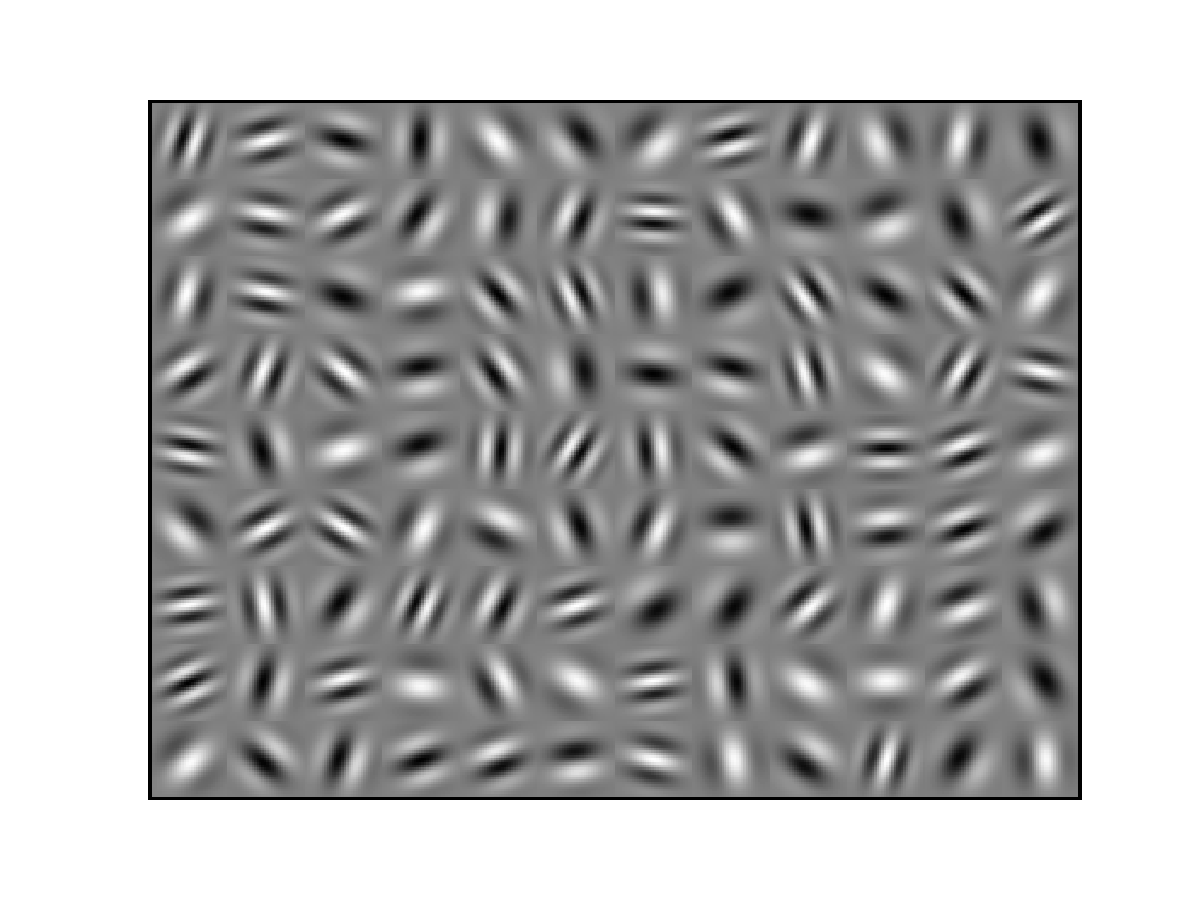
\includegraphics[width=\columnwidth]{gabors.pdf}
  \captionb{A collection of Gabor filters.}{
    Filters vary in frequency, orientation, and phase.
    $\log f \in \mathcal{U}(\log 0.5, \log 1.5)$,
    $\theta \in \mathcal{U}(-\pi, \pi)$,
    $p \in \mathcal{U}(-\pi, \pi)$, $\sigma_u = 0.45$, $\sigma_v = 0.45$.
  }
  \figlabel{gabors}
\end{figure}

\fig{gabors} shows a collection of Gabor filters.
Note that the filters vary in frequency and orientation,
such that each one is suited for detecting edges of a particular width
at a particular orientation.

Gabor filters can be combined with receptive fields,
such that each filter targets a local region of the image.
In fact, this is necessary with Gabor filters,
since edges are local features,
and Gabor filters that cover the whole image will be poorly suited
to detecting them.
It is important to note that the RFs in this case should not be thought of
as a mask, however;
that is, I do not generate full-field Gabor filters,
then use a RF mask to make them local.
Rather, I generate Gabor filters of the desired RF size,
and centre each of these on random points in the image.
Note that the parameters for the Gabor filters are in terms of the coordinates
$x$ and $y$,
which are on the interval $(-1, 1)$
independent of the size of the receptive field.
Changing the receptive field for the Gabor filter encoders
will scale all filters,
thus changing the statistics relative to the image size.


\subsection{Computed Input Weights (CIW)}

\emph{Computed Input Weights} (CIW) is a technique developed by \textcite{Tapson2015}
for generating the input weights (encoders) for a SLFN.
Unlike the previous methods presented here,
which are independent of the training data
(aside from hyperparameters which can be tuned to the data),
this method generates encoders based directly on the training dataset.
Each encoder is chosen as a weighted sum of all the examples
belonging to a particular class,
where weights are randomly chosen from the set of $\{+1, -1\}$.
Thus, each encoder targets a particular class,
but is sensitive only to some examples in that class,
and inversely sensitive to others.
Encoders are chosen to target all the classes in the dataset.
Since the weights on the in-class examples are randomly chosen,
this technique has elements of both random and data-driven encoder generation.

Given $\mat X$, an $M \times D$ matrix of training examples,
where each example belongs to one of $n_c$ classes $c \in C$,
perform the following steps to generate the $N \times D$ encoder matrix $\mat E$:
\begin{enumerate}
  \item For generating the encoders,
    use a normalized version of the training data
    with the mean over all examples and dimensions subtracted out,
    and divided by the standard deviation over all examples and dimensions.
  \item For each class in the dataset, generate $N_c = N / n_c$ encoders,
    using the following procedure:
    \begin{enumerate}
      \item Select $\mat X_c$, an $M_c \times D$ matrix of the set of examples
        that belong to the current class $c$.
      \item Generate a $M_c \times N_c$ random matrix $\mat R_c$
        where each element is either $+1$ or $-1$ with equal probability.
      \item Generate the encoders for the class as $\mat E_c = \mat R_c^T \mat X_c$.
        The full set of encoders $\mat E$ is the concatenation of $\mat E_c$
        for all classes $c \in C$.
    \end{enumerate}
  \item Normalize the encoders $\mat E$ by dividing by each row (each encoder)
    by its $L_2$ (Euclidean) norm.
\end{enumerate}


\subsection{Constrained Difference weights (CD)}

The \emph{Constrained Difference} (CD) algorithm \parencite{Zhu2015}
is another recent technique for generating SLFN encoders
using both data-driven and random elements.
Each encoder is formed as the difference between two training examples
from different classes.
Thus, each encoder tries to separate between two classes.

Given $\mat X$, an $M \times D$ matrix of training examples,
where each example belongs to one of $n_c$ classes $c \in C$,
perform the following steps $N$ times
to generate the $N \times D$ encoder matrix $\mat E$
and bias vector $\vect b$:
\begin{enumerate}
  \item Pick two different classes $a, b \in C$ randomly.
  \item Pick two random examples $\vect x_a$ and $\vect x_b$,
    belonging to the classes $a$ and $b$ respectively.
  \item Let the encoder weight
    $\vect w = 2 (\vect x_a - \vect x_b) / \|\vect x_a - \vect x_b\|_2$,
    and bias $b = (\vect x_a - \vect x_b)^T (\vect x_a + \vect x_b) / \|\vect x_a - \vect x_b\|_2$.
\end{enumerate}


\section{Decoding methods}
\scnlabel{nef-decoding}

Another key question with fixed-encoding methods
is how to find decoding weights.

At the core of this question is the choice of loss function,
which defines the objective that we wish to minimize
(see \scn{objective-functions} for an overview of loss functions).
For classification, we ultimately wish to minimize the classification error,
that is, the number of examples incorrectly classified.
However, the classification error is a discrete value,
prohibiting us from using it directly \parencite{Toh2008}.
For example, if we make a small change to our model,
it may not change how any example in our training set is classified,
and thus the classification error does not change.
Yet, we need to know whether this change is an improvement or not;
it may move some incorrectly classified examples
closer to being correctly classified,
and many changes in that same direction may lead to better classification error.
The idea behind loss functions for classification
is to find a continuous value---the loss---%
which when minimized will also minimize the classification error.

Many classification loss functions were originally formulated
for binary classification, where we have only two output classes.
In object classification, there are typically many different classes,
since there are many types of objects in the world.
Thus, we are interested in loss functions
for multiclass classification,
where we have more than two classes.

I focus on loss functions that result in a linear classifier.
Given an $M \times N$ matrix of hidden node activations $\mat A$
(found by applying the encoders and neural nonlinearity to the training data points),
we wish to find an $N \times C$ matrix of decoding weights $\Dec$
that map the hidden neuron activations to outputs $\mat Y$:
\begin{align}
  \mat Y = \mat A \Dec \text{ .}
\end{align}
$\vect y_k$ represents one row of $\mat Y$,
that is, the output of the system for training example $k$;
$\dec_i$ represents one column of $\Dec$,
that is, the decoders for one of the $C$ output dimensions.
In training this classifier we use either the vector of labels $\vect l$
for the $M$ training examples,
or the equivalent one-hot representations $\mat T$,
an $M \times C$ matrix where
\begin{align}
  T_{ki} = \begin{cases}
    1 & \text{if } i = c(k) \\
    0 & \text{otherwise}
  \end{cases} \text{ ,}
\end{align}
$c(k)$ is the correct class (label) for example $k$,
and $\vect t_k$ is one row of this matrix (\ie/ the one-hot encoding of example $k$).

My main reason for using a linear classifier
is that it can be directly mapped onto neural connection weights.
Note that this does not mean we are limited to linear optimization methods;
two of the loss functions examined here (softmax loss and hinge loss)
require nonlinear optimization,
yet result in a linear classifier.
Also, when used as part of a larger neural system,
the classifier may connect directly into nonlinear components,
such that the entire system forms a type of nonlinear classifier.
For example, the classifier may connect into a system like
the basal ganglia,
which chooses the maximum output of the classifier
and routes information accordingly.

Loss functions have been explored extensively
in machine learning \parencite[\eg/][]{Rosasco2004},
and it is known that squared loss
is not optimal for classification \parencite[][p. 186]{Bishop2006}.
Yet, these loss functions are typically not used in the ELM literature
\parencite[\eg/][]{McDonnell2015}.
A notable exception is the work of \textcite{Toh2008},
who introduces weighted squared loss for ELMs.
This section explores loss functions in the context of SLFNs,
to bring more awareness of the benefits of alternative loss functions
to researchers working with SLFNs and other fixed-encoding networks.


\subsection{Squared loss}
\scnlabel{squaredloss}

Squared loss, also known as the least-squares technique,
is common for solving regression problems.
It minimizes the sum of squared errors between each predicted point
and the corresponding target point.
%% Squared loss generalizes least squares to classification problems.
In the multiclass case it uses a one-hot encoding of the target class $\mat T$
as the target point.

The squared loss across all $M$ examples is given by
\begin{align}
  %% O_\text{MSE} = \frac{1}{N} \sum^N_k \sum_i (y^{(k)}_i - y^{*(k)}_i)^2.
  %% O_\text{MSE} = \frac{1}{M} \sum^M_k \|\vect y_k - y^*_k\|_2^2.
  O_\text{squared} = \sum^M_k \|\vect y_k - \vect t_k\|_2^2 \text{ .}
  \eqnlabel{squaredloss}
\end{align}
This amounts to training a one-vs-all classifier for each class.
We wish to find the linear decoders $\Dec$,
a matrix mapping the $N$ hidden neuron activities to the $C$ categories.
The solution to this problem, in matrix form, is
\begin{align}
  \Dec = (\mat A^T \mat A)^{-1} \mat A^T \mat T.
  \eqnlabel{lstsq}
\end{align}
This is found by taking the derivative of \eqn{squaredloss}
and setting it equal to zero to find the stationary points.
Because the objective function is quadratic,
the single stationary point is necessarily a minimum.

Squared loss is not ideal for classification,
since it leads to slower convergence than softmax loss and hinge loss
\parencite{Rosasco2004},
and often results in sub-optimal classification boundaries \parencite[][p. 187]{Bishop2006}.
Part of the reason for this is that it penalizes outliers heavily,
such that larger errors are much more costly than smaller ones \parencite[\eg/][p. 186]{Bishop2006}.
For example, consider a classifier that has two outputs,
corresponding to two different classes.
Say we have two examples that are both labeled as the first class:
their one-hot target vectors will both be $\vect y^* = [1, 0]$.
If the classifier outputs $y_1 = [1, 0.9]$ for the first example,
it has correctly classified it
by a margin of 0.1 (the difference between the correct category output
and the next highest output).
The loss on this example is $\|y_1 - y^*\|_2^2 = (0.9)^2 = 0.81$.
Say for the other example (of the same category),
the classifier outputs $y_2 = [0.4, 0.6]$.
It has incorrectly classified this example by a margin of 0.2.
The loss on this example is $\|y_1 - y^*\|_2^2 = (-0.6)^2 + (0.6)^2 = 0.72$.
Therefore, the classifier does better on the first example,
but the loss is lower on the second example.
This is the opposite of what we want!

Another related problem becomes apparent as we move to more classes.
This problem is that the loss function over-penalizes when
there are multiple competing classes.
Consider a classifier that has three outputs;
again, we look at two examples from the first class,
thus with one-hot target vector $\vect y^* = [1, 0, 0]$.
If the output for the first example is $y_1 = [1, 0.8, 0.8]$,
and for the second example is $y_2 = [0.8, 1, 0]$,
the loss for the first example is $2 (0.8)^2 = 1.28$
and for the second example $(-0.2)^2 + (1)^2 = 1.04$.
The first example is correctly classified by a margin of 0.2,
whereas the second is incorrectly classified by a margin of 0.2,
but the second example has the smaller loss.
The difference between the two examples is that
the first has significant errors in two outputs (outputs two and three),
whereas the second only has a significant error in the second output.
The loss function penalizes the case where many classes have significant errors,
even though this is often not a problem as long as the correct class
is beating all other classes by a significant margin.

These problems both occur because the classifier is treating each element
of the target vector as an independent regression variable.
To achieve better results
requires some sort of dependence
between the outputs for these regression variables.


\subsection{Weighted squared loss}
\scnlabel{wsquaredloss}

To address the problem that linear least squares
over-penalizes multiple competing classes,
I investigated weighting errors on examples of the target class (positive examples)
more heavily than those of other classes (negative examples).
If we view each output dimension of the classifier
as an independent one-vs-all classifier---%
which is how linear least squares treats the problem---%
then it is intuitive that for each one-vs-all classifier,
we want a balance between positive and negative examples.
Re-weighting the examples achieves this balance.

\textcite{Toh2008} came to a similar conclusion,
from a more theoretical basis.
They derived the same weighted least squares solution
by approximating the discontinuous classification error as best possible
with a quadratic function.
Despite this significant result,
many modern SLFNs still use unweighted linear least squares \parencite{McDonnell2015}.

Weighted least squares is a popular variant of least squares
whereby different residuals can be given different weights.
If there is measurement uncertainty (error)
associated with each of the regression points,
and this uncertainty varies between points and can be quantified,
weighted least squares allows one to account for this uncertainty \parencite{Fieguth2010}.

Linear weighted least squares is defined by a similar objective function
to ordinary linear least squares (\eqn{squaredloss}),
except with scalar weights $w_k$ on each error:
\begin{align}
  \left[O_\text{w-squared}\right]_i = \sum^M_k w_k (Y_{ki} - T_{ki})^2.
  \eqnlabel{wsquaredloss}
\end{align}
It is defined here for the one-dimensional case (\ie/ for output dimension $i$),
to allow for separate weights for each dimension of the output,
based on whether that dimension represents the correct or incorrect class
for each example (see below).
%% \begin{align}
%%   \vect x = \argmin_x \sum_k w_k r_k^2
%%   \text{, where } r_k = A_k \vect x - y_k
%%   \eqnlabel{wlstsq-obj}
%% \end{align}
%% for the one-dimensional case.

Taking the derivative and setting it equal to zero, as before, we find that:
\begin{align}
  \Dec = (\mat A^T \mat W \mat A)^{-1} \mat A^T \mat W \vect T_{\cdot i}
\end{align}
where $\mat W$ is a square diagonal matrix of the weights $w_k$
and $\vect T_{\cdot i}$ is column $i$ of $\mat T$.
This system can be solved using the same solution as for unweighted least squares,
including SVD if the system is ill-conditioned,
and Cholesky decomposition if it is well-conditioned.

We can weight examples based on their frequency,
such that the (typically less frequent) positive examples
receive the same total weight as the negative examples:
\begin{align}
  n^+ w^+ = n^- w^-
\end{align}
where $n^+$ and $n^-$ are the numbers of positive and negative examples,
and $w^+$ and $w^-$ are the weights on the positive and negative examples.
We also wish the total weight to sum to the number of examples:
\begin{align}
  n^+ w^+ + n^- w^- = n^+ + n^- \text{ .}
\end{align}
This results in weights
\begin{align}
  w^+ &= \frac{1}{2p^+} \\
  w^- &= \frac{1}{2(1 - p^+)}
\end{align}
where $p^+ \equiv n^+ / (n^+ + n^-)$ is the fraction of positive examples.
If both categories appear equally frequently (\ie/ $p^+ = 0.5$),
then $w^+ = w^- = 1$,
and the method is equivalent to unweighted least squares.

The key to this method is that this weighting is different
for each one-vs-all classifier,
such that each one requires solving a different linear system.
Specifically,
in the case of unweighted least squares,
we can solve
%% $\Dec = (\mat A^T \mat A + \lambda \mat I)^{-1} \mat A^T \mat T$
$\Dec = (\mat A^T \mat A)^{-1} \mat A^T \mat T$
simultaneously for all columns of $\mat T$.
With weighted least squares method we must solve
\begin{align}
  %% \Dec_{\cdot,i} = (\mat A^T \mat W_i \mat A + \lambda \mat I)^{-1} \mat A^T \mat W_k \mat T_{\cdot,i}
  \Dec_{\cdot,i} = (\mat A^T \mat W_i \mat A)^{-1} \mat A^T \mat W_k \mat T_{\cdot,i}
\end{align}
where $\Dec_{\cdot,i}$ and $\mat T_{\cdot,i}$ are the $i$\sth/ columns of $\Dec$ and $\mat T$,
and $\mat W_i$ is a unique set of weights for each value of $i$.
Luckily, structure in the weights allows us to solve these systems
with the same order of computation
as solving the unweighted least squares system (see \app{wlls}).


\subsection{Softmax loss}
\scnlabel{softmaxloss}

The softmax loss (also known as the logistic loss or cross-entropy loss)
allows us to better model the max function that our classifier output
passes through when determining the classification error.
In the multiclass case,
we pass the linear classifier output through the softmax function,
which normalizes the outputs relative to one another.
The softmax function is so named because it is a
differentiable (``soft'') version of the max function.

The softmax loss is given by
\begin{align}
  O_\text{log} &= -\sum_k^M \left[\log (\vect\sigma(\vect y_k))\right]_{c(k)}
\end{align}
where $c(k)$ is the label index of the $k$\sth/ example,
and $\vect\sigma$ is the softmax function
\begin{align}
  \vect\sigma(\vect y) = \frac{e^{\vect y}}{\sum_i e^{y_i}} \text{ .}
\end{align}
The derivative of the softmax loss function is surprisingly simple:
It is simply the error difference between the output of the softmax function
and the target one-hot representation:
\begin{align}
  \diff{O_\text{log}}{\vect y_k} &= \vect\sigma(\vect y_k) - \vect t_k \\
  \diff{O_\text{log}}{\Dec} &= \mat A^T \diff{O_\text{log}}{\mat Y} \text{ .}
\end{align}
Despite the simplicity of this derivative,
it is still nonlinear, due to the softmax function.
Therefore, we have to solve using nonlinear optimization techniques.
The L-BFGS method \parencite{Liu1989} works quite well.\footnote{
  Using the implementation in Scipy: \url{http://www.scipy.org}}

The softmax loss is closely related to the classification error.
If an example is correctly classified,
then the softmax loss is necessarily lower on that example
than if it is incorrectly classified.
That is, the softmax loss can never be higher for a correctly classified example
than for an incorrectly classified one.
Compare this with squared loss,
which we saw by example in the previous section could have lower loss
for incorrectly classified examples than for correctly classified ones.
This does not mean, however, that minimizing the softmax loss
will necessarily result in the best possible linear classifier.
For example, if one example is misclassified by the classifier by a huge margin,
resulting in a huge loss,
this could be a higher total loss than a number of examples
that are only misclassified by a small margin.
Such a situation can happen with outliers,
where one training example looks very different than other members of its class,
or with incorrectly labeled data (\ie/ noisy labels).
Thus, even with softmax loss,
the lowest loss does not result in the lowest training-set classification error.
However, the relationship between loss and classification error
is much closer than with squared loss.


\subsection{Hinge loss}
\scnlabel{hingeloss}

Hinge loss maximizes the margins between the correct class and incorrect class
for all the training examples,
with a maximum margin at which we consider two examples perfectly distinguished.
This is the loss traditionally associated with support vector machines.
%% That is, in the binary classification situation,
%% we want the margin between the co

There is no unique way to generalize hinge loss to the multiclass problem.
One choice is to maximize the margin of the correct class
over the next highest class \parencite{Crammer2001}.\footnote{
  This is the formulation used here.
  A comparison of formulations of hinge loss is beyond the scope of this thesis.}
For example $k$, the margin $m_k$ is given by:
\begin{align}
  m_k = Y_{kc} - \max_{i \ne c} Y_{ki}
\end{align}
where $c$ is the correct class for example $k$,
$Y_{kc}$ is the classifier output for the correct class,
and $Y_{ki}$ is the classifier output for one of the incorrect classes $i$.
Of course, this margin can be negative if the correct class $c$
does not have the highest response
(in which case the classifier is incorrectly classifying example $k$).
Our objective function is
\begin{align}
  O_\text{hinge} = \sum_k \max\left(0, 1 - m_k\right) \text{ .}
\end{align}
Any example that has a margin $\ge 1$ is considered ideally classified,
and has zero loss.
The loss for all other examples is one minus the margin.

The derivative of this hinge loss with respect to the classifier output is
\begin{align}
  \diff{O_\text{hinge}}{Y_{ki}} = \begin{cases}
    -1 & \text{if } i = c \\
    1 & \text{if } i = a \\
    0 & \text{otherwise}
  \end{cases}
\end{align}
That is, increasing $Y_{kc}$ will decrease the loss,
and increasing $Y_{ka}$ will increase the loss,
where $a = \argmax_{i \ne c} Y_{ki}$ is the highest response not of the correct class.
We can then find the derivative with respect to the classifier weights
by using the chain rule:
\begin{align}
  \diff{O_\text{hinge}}{\Dec} &= \mat A^T \diff{O_\text{hinge}}{\mat Y} \text{ .}
\end{align}

One important aspect of the hinge loss is that it is
very dependent on the magnitude of the classifier outputs $\mat Y$,
and by extension the decoding weights $\Dec$.
For example, if the classifier has many examples correct by a given margin,
doubling the classifier weights will double that margin for all correct examples.
For this reason, most support vector machines that use hinge loss
also use a constraint on the magnitude of the weight vector,
typically an equality constraint ensuring it has a norm of one.
I have not employed such a constraint,
but rather used regularization on the weight magnitude
to a similar effect (see \scn{dec-regularization}).
Though other loss functions (\eg/ softmax loss)
can also be vulnerable to situations where larger magnitudes yield lower loss,
this effect seems the most prominent with hinge loss (see \fig{nef-regularization}),
and thus regularization is particularly important with this loss function.

Like the softmax loss,
the hinge loss function has the benefit
that it is closely related to the classification error.
If an example is correctly classified,
then the hinge loss for that example is necessarily lower
than if the example is incorrectly classified.
This makes it a better loss function than the squared loss.

% Lee2004?? I put this here before, but I can't remember why


\subsection{Weight norm regularization}
\scnlabel{dec-regularization}

Adding a cost on the magnitude of the weights
can both help with overfitting,
and can help reduce noise when using spiking neurons \parencite{Eliasmith2003}.
This is not a cost or loss function by itself,
but rather a term that can be added to any other loss function.

Given an objective function $O$,
we can create a regularized version $O_\text{reg}$:
\begin{align}
  O_\text{reg} = O + \lambda \|\Gamma \Dec\|_p
\end{align}
where $\Dec$ is the set of parameters (weights) being learned.
Thus, we are taking the $L_p$ norm on a linear projection $\Gamma$ of our weights.
Often, we take $\Gamma$ to be a scalar multiple of the identity matrix,
such that we are simply minimizing the norm of the weights themselves.

If we also take the norm to be the $L_2$ (Euclidean) norm,
we get \emph{ridge regression}:
\begin{align}
  O_2 = O + \frac{\lambda}{2} \|\Dec\|_2^2.
\end{align}
This penalizes the sum of squared elements of $\Dec$.
It is particularly useful when combined with linear least squares,
since its derivative is also linear, thus still allowing a linear solution.

If we instead take the norm to be the $L_1$ (Manhattan) norm,
we get the \emph{lasso}:
\begin{align}
  O_1 = O + \lambda \|\Dec\|_1.
\end{align}
This results in sparse $\Dec$, where many elements are zero.

Here, I focus on $L_2$ norm regularization,
mainly because it can be used with squared loss functions
and still allow analytic solutions
(thus accelerating the decoder-finding process).
The $L_2$ norm was also used by \textcite{Eliasmith2003}
to reduce the amount of variance from spikes in the output of a spiking network,
and thus has benefits specific to spiking networks.

The effect that regularization will have depends on
the scale of the activity matrix $\mat A$.
Because I have written my loss functions as taking
the sum of the losses on all points, rather than the mean,
the effect of regularization also depends on the number of points $M$.
Thus, I scale the regularization constant $\rho$
by both the maximum activity $\|\mat A\|_\infty$ and by $M$,
to yield the total regularization parameter $\lambda$:
\begin{align}
  \sigma &= \rho \|\mat A\|_\infty \\
  \lambda &= M \sigma^2
\end{align}
By squaring $\sigma$, this equation is tuned for use with an $L_2$ norm.
%% Determining the regularization constant for an $L_1$ norm

% introduce LOO cross-validation, either here or maybe in intro? Probably in intro
Determining the regularization parameter $\rho$ is not trivial.
Cross-validation techniques estimate the generalization error of a method on a dataset;
by applying the cross-validation technique for many different $\rho$ values,
one can determine a near-optimal choice for $\rho$.
Leave-one-out (LOO) cross-validation computes the classifier on all data points
except one, then computes the classification error on the excluded data point.
Repeating this for all data points yields a robust estimate of the generalization error.
Unfortunately, it scales linearly with the number of training data points,
making it very costly for our application (where solving for the classifier is costly).
Other possible cross-validation methods include using a number of randomly-selected
subsets from the dataset for each $\rho$ value,
or taking a single subset of the training data and holding it aside as a validation set.

% talk about Rifkin2007 method
\textcite{Rifkin2007} demonstrated that the regularization parameter
can be found using leave-one-out (LOO) cross-validation
at little extra cost when using direct least-squares solution methods.
They derived an expression for the LOO error
that depends only on the eigendecomposition of
the covariance matrix ($\mat A^T \mat A$) of the system
(they also derive the same result using the singular value decomposition of $\mat A$).
Using this method, the effect of different values of $\rho$ on the LOO error
to be tested without re-solving the system itself,
and a good value for the regularization parameter
can be found at (theoretically) little extra cost.

The core of the method is the fact that for a linear least-squares problem,
as formulated in \eqn{lstsq} (with regularization),
the vector of LOO errors $\vect e_\text{LOO}$
for each training sample is given by
\begin{align}
  \vect e_\text{LOO} = \frac{
    \mat Y - \mat A (\mat A^T \mat A + \lambda\mat I)^{-1} \mat A^T \mat Y}{
    \diag(I - \mat A (\mat A^T \mat A + \lambda\mat I)^{-1} \mat A^T)}
  \eqnlabel{rifkin}
\end{align}
where $\diag(\mat X)$ is the vector of diagonal elements of matrix $\mat X$,
and the division is performed elementwise.
The covariance matrix can be factored using an eigendecomposition,
\ie/ $\mat A^T \mat A = \mat Q \Lambda \mat Q^T$,
where $\mat Q$ is an orthogonal matrix and $\Lambda$ is a diagonal matrix.
Thus, $(\mat A^T \mat A + \lambda\mat I)^{-1} = \mat Q (\Lambda + \lambda)^{-1} \mat Q^T$.
This allows us to re-write \eqn{rifkin} as
\begin{align}
  \vect e_\text{LOO} &= \frac{
    \mat Y - \mat A \mat Q (\Lambda + \lambda\mat I)^{-1} \mat Q^T \mat A^T \mat Y}{
    \diag(I - \mat A \mat Q (\Lambda + \lambda\mat I)^{-1} \mat Q^T \mat A^T)}
  \eqnlabel{rifkin-eigen} \\
  &= \frac{
    \mat Y - \mat P (\Lambda + \lambda\mat I)^{-1} \mat P^T \mat Y}{
    \diag(I - \mat P (\Lambda + \lambda\mat I)^{-1} \mat P^T)}
\end{align}
where $\mat P = \mat A \mat Q$.
The denominator $\vect d$ of this expression can be calculated efficiently as
\begin{align}
  d_i = \sum_j^N \frac{P_{ij} P_{ij}}{\Lambda_{jj} + \lambda}.
\end{align}
Unfortunately, this computation still involves computing the matrix product
$\mat P = \mat A \mat Q$, which is $O(MN^2)$.
Using the form of \eqn{rifkin-eigen} is no better:
while the numerator can be computed
as four successive $O(MNC)$ products with the matrix $\mat Y$,
the denominator involves an unavoidable $O(MN^2)$ matrix-matrix product,
which is more expensive since $C \ll N$.
Furthermore, when using this method with the weighted squared loss,
we need to form $\mat P$ again for each weighting,
since the weighting affects the value of $\mat Q$.
Thus, the cost of this method is $O(CMN^2)$ for weighted least squares.
Unfortunately, this method only works for squared loss functions,
and does not generalize to softmax loss or hinge loss.


\section{Spiking methods}
\scnlabel{nef-spiking-methods}

Simulating a network with spiking neurons
is different than running an ANN with rate neurons.
Spiking neurons are dynamic and must be run \emph{online},
with each stimulus (image) presented for a period of time
such that the spiking neurons have time to respond with a spike train signal.
ANNs---on the other hand---are almost always run offline,
presenting as many images to the network at a time as desired,
and responses for all images generated with a single forward pass
through the network.\footnote{
  This assumes the networks are fully feedforward,
  as are all the networks presented and discussed in this thesis.
  Recurrent networks require presenting inputs over a span of time.}
This change from offline to online introduces a number of new design decisions.

One of the most important design decisions
is how the classification is performed.
In biological systems, when we examine the macro-level behaviour of the system,
we are always looking at the full system,
from the external stimulus (image) to the physical response
(motor movement or speech).
The network presented here does not include a motor system
to close this behaviour loop,
so when we evaluate it based on its output,
we do not get the full picture of how it would operate
in a closed-loop system.

For the evaluation of the spiking networks in this thesis,
the category selected by the classifier
is the category with the maximum average response
during the presentation of each stimulus.
The advantages of this approach are that it is simple,
it captures how the system would perform on a neuromorphic chip,
and it allows for a fair comparison with current machine-learning approaches.
The main disadvantage is that selecting the maximum of a number of values
is not a function that can be computed perfectly or easily in neurons,
particularly when there are multiple values near the maximum.
The Spaun brain model \parencite{Eliasmith2012}
uses a detailed model of the basal ganglia to compute this operation.
Such a basal ganglia model could be included
as part of the networks presented here,
to get a better idea of how they might function as part of an end-to-end system.

There are three new hyperparameters associated with running our network online
in spiking neurons, that do not appear in the offline network:
\begin{enumerate}
  \item The presentation time $t_p$ that each stimulus is shown for,
  \item the classification start time $t_c$,
    which determines how long after the stimulus is first presented
    the averaging for classification starts, and
  \item the time constants $\taus$ of any synapses in the network.
\end{enumerate}
In terms of accuracy, a longer presentation time is always better,
since it allows more time for any transient dynamics in the network to settle
and for the output to average across a larger time window,
thus reducing some of the variability associated with spiking neurons.
In practice, choosing the presentation time
is always a tradeoff between accuracy and throughput,
where shorter presentation times allow more stimuli to be classified
per unit time,
at the cost of accuracy.

The classification start time determines at what point after each stimulus is shown
do we begin averaging the network outputs for classification.
This allows the classifier to ignore the initial transient output of the network.
It is important because I test these networks continuously
over the whole series of test inputs,
preserving the network state from one input to the next.
Some other works \parencite[\eg/][]{Cao2014,Diehl2015} present each stimulus separately,
resetting the state of the network between presentations;
in that setup, there is no transient state from previous presentations,
so using the whole presentation time for classification is not problematic.

Finally, the synapse time constants determine the amount of filtering
applied to the output of each neuron.
For the networks in this chapter,
which only have a single hidden layer,
then this is equivalent to filtering on the output (since the classifier is linear).
For the deep networks examined in later chapters,
the filtering is applied to the output of \emph{each} neuron layer.
All networks in this thesis use alpha synapses (\eqn{alpha-synapse}).
The time constants of the synapses affect the amount of time required
for information to propagate through the network,
and thus the value of the time constant (combined with the network depth)
should be the main factor determining the choice
of the classification start time $t_c$.

For the networks in this chapter,
I chose $t_p = 70$ ms, $t_c = 5$ ms, and $\taus = 0$ ms.
This allows sufficient time to classify each input accurately
while still allowing the network to process images quickly.
Since the networks only have a single hidden layer
and the classification method already averages over their output,
I found that synaptic filtering was unnecessary.

All simulations were performed using the Nengo neural simulator \parencite{Bekolay2014}.


%%%%%%%%%%%%%%%%%%%%%%%%%%%%%%%%%%%%%%%%%%%%%%%%%%%%%%%%%%%%%%%%%%%%%%%%%%%%%%%%
\section{Results}

To assess the performance of the encoding and decoding methods
described in this chapter,
I used the MNIST dataset as a benchmark.


\subsection{Encoding}
\scnlabel{enc-results}

\begin{figure}
  \centering
  \newcommand{\gwidth}{0.45\columnwidth}
  \begin{tabular}{cc}
    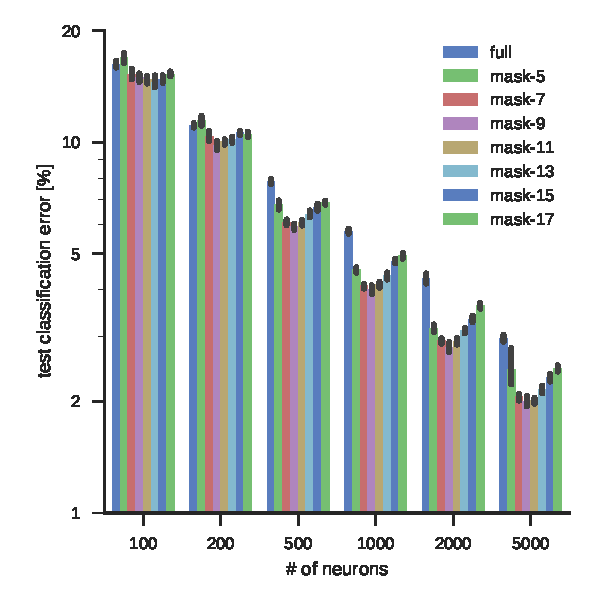
\includegraphics[width=\gwidth,clip=true,trim=3mm 3mm 3mm 3mm]{mnist_compare_encoders_masks.pdf} &
    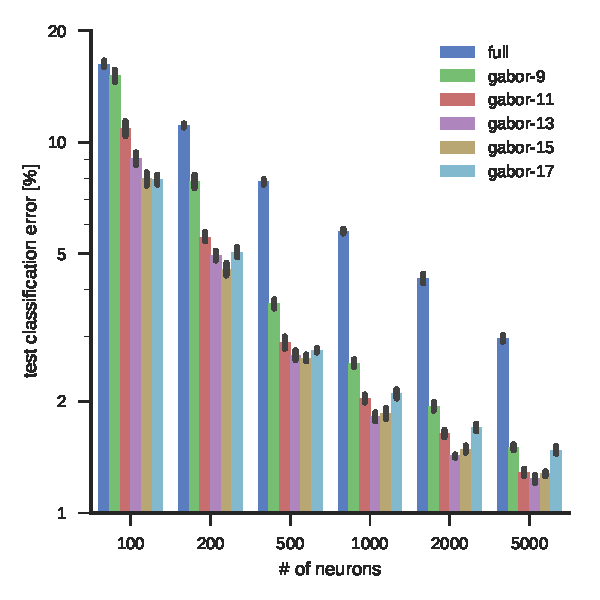
\includegraphics[width=\gwidth,clip=true,trim=3mm 3mm 3mm 3mm]{mnist_compare_encoders_gabors.pdf} \\
    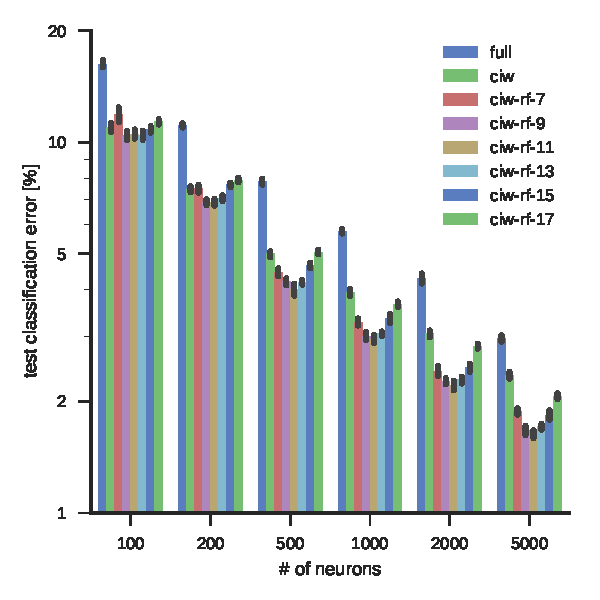
\includegraphics[width=\gwidth,clip=true,trim=3mm 3mm 3mm 3mm]{mnist_compare_encoders_ciw.pdf} &
    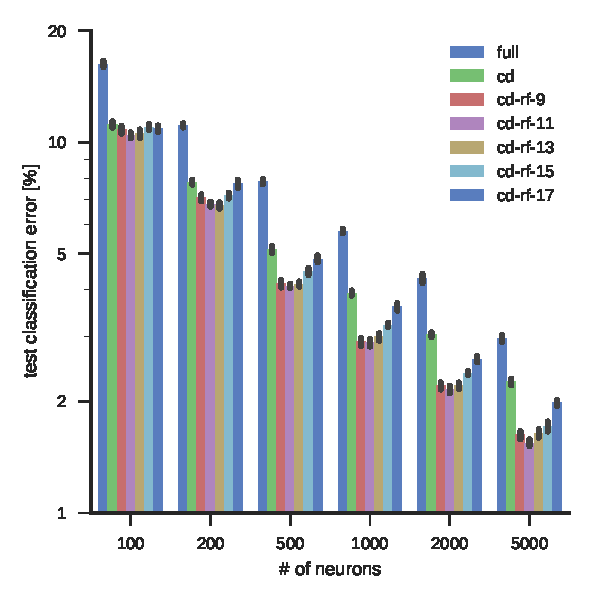
\includegraphics[width=\gwidth,clip=true,trim=3mm 3mm 3mm 3mm]{mnist_compare_encoders_cd.pdf} \\
  \end{tabular}
  \captionb{Different choices of encoders for SLFNs.}{
    \textbf{Top left:} Using limited receptive fields (``mask-\#'') reduces
    test-set error vs fully-connected random encoders (``full'').
    RFs around the $9 \times 9$ size perform the best.
    \textbf{Top right:} Using Gabor filters with varying sizes of RFs (``gabor-\#'')
    also reduces test-set error, with $13 \times 13$ RF size working best.
    The Gabor filter parameters are:
    $f \in \mathcal{U}(0.2, 2.0)$,
    $\theta \in \mathcal{U}(-\pi, \pi)$,
    $p \in \mathcal{U}(-\pi, \pi)$, $\sigma_u = 0.45$, $\sigma_v = 0.45$.
    \textbf{Bottom left:} CIW encoders also improve performance,
    with a $11 \times 11$ RF size working best.
    \textbf{Bottom right:} CD encoders also follow the trend,
    again with $11 \times 11$ RF size working best.
    %% \# indicates the receptive field size.
  }
  \figlabel{nef-encoder-choices}
\end{figure}

\fig{nef-encoder-choices} shows detailed results
for each of the four methods examined.
In the figure, ``full'' refers to fully connected,
independent and identically distributed (i.i.d.) random encoders,
which generally perform the worst.
Adding a receptive field (RF) mask to i.i.d. random encoders (``mask-\#''),
such that each encoder is only connected to a limited local region of the image,
improves performance.
There are some receptive field sizes, such as $3 \times 3$ (not shown),
for which the RF i.i.d. encoders perform worse than fully connected ones.
Other, non-i.i.d. methods of generating encoders can be combined
with receptive fields to improve performance.
With Gabor filters, using a RF size of $13 \times 13$ works best.
Full-field Gabor filters perform poorly (not shown),
because edges are local features,
and thus filters for detecting them must also be local.
Finally, the RF method can be combined with the CIW and CD methods
to improve their performance;
this supports the results of \textcite{McDonnell2015}.


\begin{figure}
  \centering
  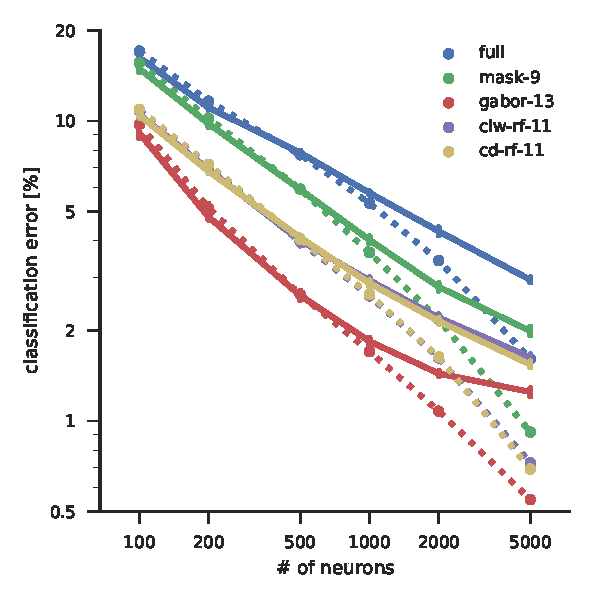
\includegraphics[width=4in]{mnist_compare_encoders_besttt.pdf}
  \captionb{Encoder choices for SLFNs with optimal RF size.}{
    Training-set error (dotted line) and test-set error (solid line)
    for the five encoding methods,
    using the optimal RF sizes as determined by \fig{nef-encoder-choices}.
    The number in each label indicates the RF size.
  }
  \figlabel{nef-encoder-summary}
\end{figure}

\fig{nef-encoder-summary} shows the result of testing a number of different methods
of choosing encoders.
Encoder choice has a significant effect on test error rates.
Using i.i.d. encoders with limited receptive fields (RFs),
results in significantly better performance than fully connected i.i.d. encoders,
if the size of the RFs is chosen well.
The data-driven CIW and CD methods again offer some improvement,
though surprisingly it is the Gabor filter encoders that perform the best.

It is not surprising that Gabor filters perform better
than the i.i.d. methods.
Gabor filters are good at sparsely representing natural images \parencite{Olshausen1996},
and most deep networks that perform well on real-world object classification tasks
have been found to have something like Gabor filters in the first layer \parencite[\eg/][]{Krizhevsky2012}.
These results show that the Gabor filters do not have to be
individually tuned to the data;
a wide range of filters covering the frequencies and orientations
observed in the input data
is able to achieve high levels of accuracy on MNIST.
It is surprising is that Gabor filter encoders
outperform the CIW and CD methods,
despite the latter being tuned specifically to the MNIST dataset.

The optimal size of receptive field (RF) varied depending on whether the
encoders were i.i.d. or Gabor filters.
Larger RFs worked better with Gabor filters.
This could be because Gabor filters already have a windowing aspect to them,
since they are multiplied spatially by a Gaussian amplitude function.
This creates an effective RF for the Gabor filters that is
smaller than the full RF of the filters;
that is, the pixels at the edges of the filters have low weights,
and have little effect on the filter response.
The effective RF for the Gabor filters is thus closer
to the optimal i.i.d. RF
than the full RF of the Gabor filters indicates.
An additional factor is that the frequency range of the Gabor filters
was not optimized in any rigorous way.
Since the frequencies are set relative to the RF size,
varying the RF size varies the frequency spectrum of the filters.
Thus, the optimality of the $13 \times 13$ Gabor filters
might also have to do with the frequency content of those filters.



\subsection{Decoding}
\scnlabel{dec-results}

\begin{figure}
  \centering
  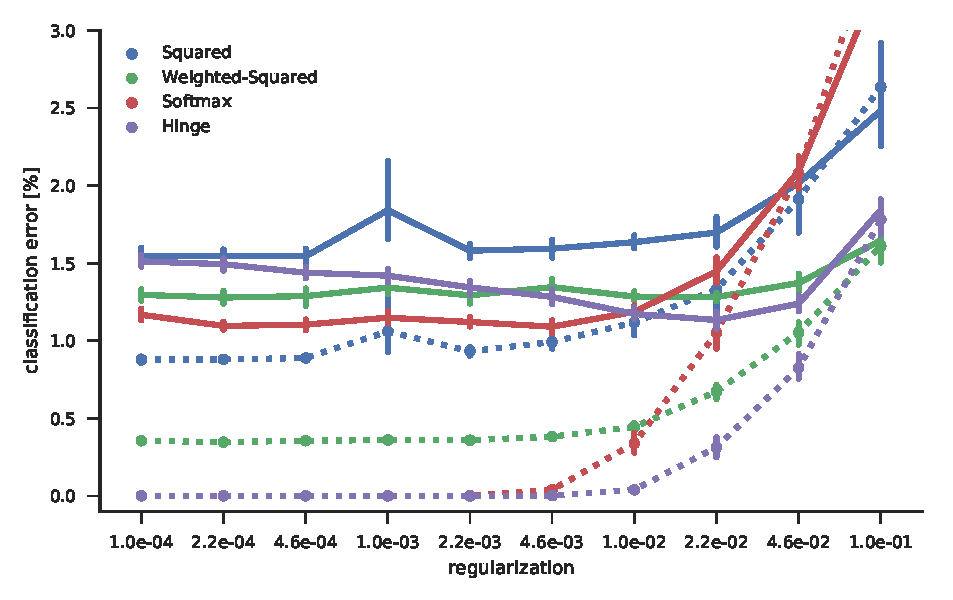
\includegraphics[width=\columnwidth]{mnist_compare_decoder_regularization.pdf}
  \captionb{Effects of regularization on different loss functions.}{
    Dotted and solid traces show training- and test-set classification errors,
    respectively.
    Some loss functions---namely squared loss and weighted squared loss---%
    show best test-set performance when regularization is negligible.
    Other loss functions---namely softmax loss and hinge loss---show
    best test-set performance for nonzero, moderate amounts of regularization.
    Error bars on test-set results show 95\% confidence intervals
    of the mean classification error across 10 trials.
  }
  \figlabel{nef-regularization}
\end{figure}

The amount of regularization has a significant effect on decoding accuracy,
such that comparing different loss functions is only informative
if the amount of regularization is also accounted for.
\fig{nef-regularization} shows the effects of the amount of regularization
on both the training- and test-set classification errors
for different loss functions.
As the figure shows,
some loss functions (least-squares and weighted least-squares)
are optimal with no regularization.
Adding regularization in small amounts has no affect on performance,
and large amounts of regularization decrease performance.
For other loss functions (softmax and hinge loss),
a moderate amount of regularization results in the best performance.
This is most evident with hinge loss,
because with hinge loss it is very easy to increase the margins
on the training data simply by increasing the magnitude of the weights,
without helping with generalization, as discussed in \scn{hingeloss}.
The reason that hinge loss and softmax
benefit from moderate amounts of regularization
is possibly because they are also the most powerful loss functions.
As shown in \fig{nef-regularization},
these loss functions are able to completely fit the training data,
achieving zero loss with low levels of regularization.
Adding regularization helps to reduce this overfitting,
leading to better generalization.

The optimal amounts of regularization for softmax loss ($\sim 4.6\times10^{-3}$)
and hinge loss ($\sim 2.2\times10^{-2}$) are quite different.
This is because these loss functions use different units.
Hinge loss is based on the margin of the correct output over the next highest output,
thus it is in the same units as the linear classifier output.
Softmax loss is the negative log probability of the correct output
after being passed through a softmax function.
Taking the log of a softmax function output
does result in a value in the same units as the linear classifier output,
but normalized by the log of the sum of all exponentiated outputs.
The result is that softmax loss has a significantly different magnitude
than the corresponding hinge loss;
the optimal amount of regularization will vary accordingly.

%% Hinge loss is shows the most variation between the
%% unregularized ($\sim$1.5\% test error) and
%% regularized ($\sim$1.1\% test error) variants.
%% This may be because the hinge loss margin depends on
%% the magnitude of the output weights.
%% Thus, even if the angle of the hyperplane defined by the output weights is not optimal,
%% a larger margin may be achievable simply by increasing the weight magnitude.
%% Applying regularization penalizes the weight magnitude,
%% forcing the optimization to find a more optimal angle for the hyperplane,
%% thus improving the generalization of the classifier.

\begin{figure}
  \centering
  %% 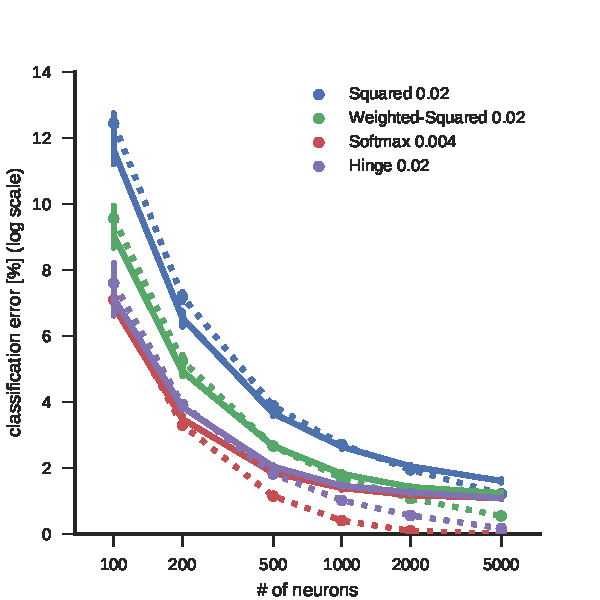
\includegraphics[width=\columnwidth]{mnist_compare_decoders.pdf}
  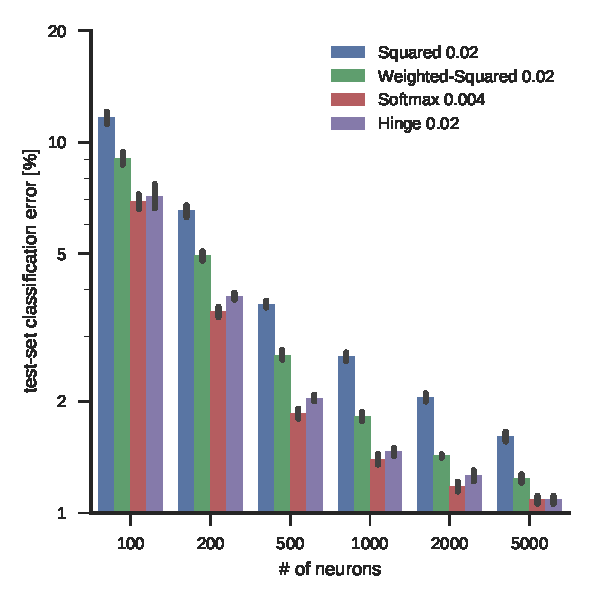
\includegraphics[width=4in]{mnist_compare_decoders_testbar.pdf}
  \captionb{Comparison of loss functions for varying numbers of neurons.}{
    The amount of regularization is chosen optimally for each loss function
    based on \fig{nef-regularization}.
    For all numbers of neurons, softmax loss and hinge loss perform the best.
    They perform equally well for large numbers of neurons,
    but softmax loss performs better for small numbers.
    This may be because the hinge loss regularization was chosen based
    on 5000 neurons, and may not be optimal for fewer neurons.
    Weighted squared loss performs significantly better than
    unweighted squared loss for all numbers of neurons,
    though never as well as softmax or hinge loss.
    Error bars show 95\% confidence intervals of the
    mean classification error across 10 trials.
  }
  \figlabel{nef-decoders}
\end{figure}

\fig{nef-decoders} compares the loss functions with optimal regularization,
across different numbers of hidden neurons.
For large numbers of neurons,
hinge loss and softmax loss perform equally well.
For fewer neurons, softmax tends to perform better,
though this result may not always be statistically significant
(see 95\% confidence interval bars).
This difference between hinge loss and softmax loss could be because
the regularization for hinge loss is chosen based on 5000 hidden neurons,
and that amount of regularization is no longer optimal for fewer neurons.
Since hinge loss is generally more affected by regularization than softmax loss
(see \fig{nef-regularization}), this would put softmax loss ahead for fewer neurons.
This could suggest that softmax loss is more robust
across varying numbers of neurons.

The other key result from this figure is that weighted squared loss
performs significantly better than its unweighted counterpart
across all numbers of neurons,
but not as well as softmax loss or hinge loss.
This can be explained by how well each loss function is able to
fit the training data (see \fig{nef-regularization}).
For lower amounts of regularization,
softmax loss and hinge loss are able to achieve almost zero classification error,
that is they are able to fully fit the training data.
The squared loss methods, on the other hand,
still misclassify many training examples,
likely due to the drawbacks of squared loss as described in \scn{squaredloss}.
However, weighted squared loss performs much better on the training data
than unweighted squared loss,
allowing it to perform better on the test data as well.


%% %% With the optimal amount of regularization,
%% hinge loss performs the best,
%% followed by softmax loss,
%% then both variants of the weighted least squares loss.
%% The plain least squares loss performs the worst,
%% considerably worse than the others.
%% Since plain least squares loss is still the norm
%% for many recent fixed-encoder networks \parencite[\eg/][]{McDonnell2015},
%% this suggests that better loss functions could considerably improve
%% current state-of-the-art results.


\subsection{Spiking}

\begin{figure}
  \centering
  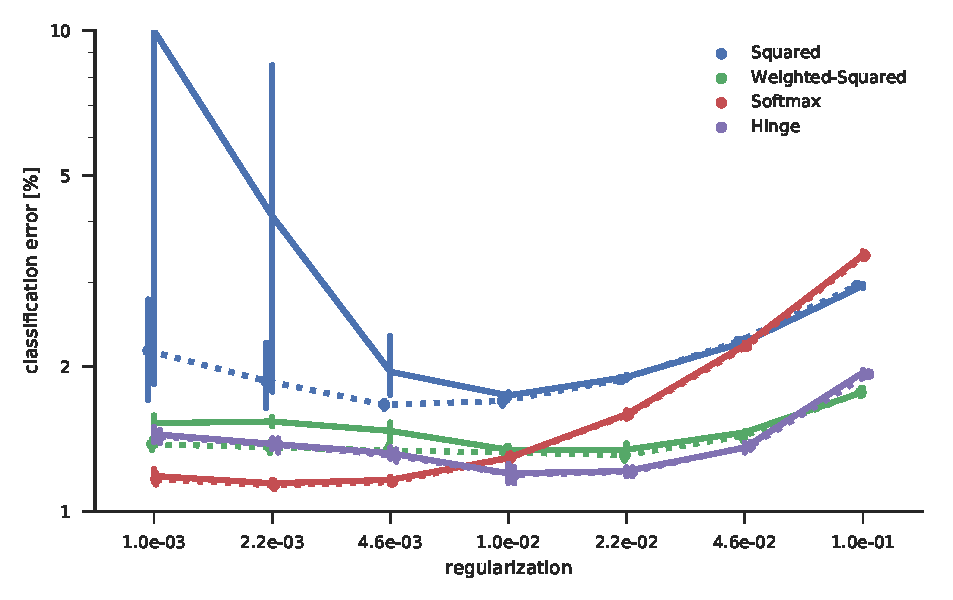
\includegraphics[width=6.35in]{mnist_compare_decoder_spiking_regularization.pdf}
  \captionb{Effects of regularization on spiking networks with 5000 hidden units.}{
    Solid lines show spiking network test-set error,
    dotted lines show rate network test-set error.
  }
  \figlabel{nef-spikingregularization}
\end{figure}

By substituting spiking LIF neurons for the rate LIF neurons used for training,
we can create networks of spiking neurons for classification.
Regularization has an even greater benefit on spiking networks,
as shown in \fig{nef-spikingregularization}.
This is because not only does regularization help with generalization
from the testing set to the training set,
it also helps reduce the variance caused by spikes
by penalizing large decoding weight magnitudes.
Large decoding weights amplify the variance caused by spiking neurons
by making the output much more dependent on some neurons over others.
When decoding weight magnitudes are more uniform---%
as encouraged by $L_2$-regularization---%
the spiking variance from different neurons tends to cancel out,
leading to less variance in the output.

Regularization is most important for the unweighted squared loss classifier
(\fig{nef-spikingregularization}, blue line).
When this loss function is not regularized,
it sometimes puts large weights on some neurons over others.
By doing so, it can better exploit some patterns it finds in the training data;
for example, one neuron having a slightly higher activation than another neuron
might indicate a particular class,
such that the amplified difference between these two neurons
can be used in the classifier.
However, pitting one neuron against another like this
is often not robust when we move to spiking neurons,
since spikes are variable and dynamic, where rates are not.
Thus, the unregularized squared loss classifier sometimes fails catastrophically,
getting $> 20\%$ error in spiking neurons
despite achieving $\sim 2\%$ error in rate neurons.
This only seems to happen one or two times in ten;
the rest of the time, the spiking error is reasonably close (within 1\%)
to the rate-neuron error.
This occasional catastrophic failure is why the unregularized squared loss
has such high mean errors in \fig{nef-spikingregularization},
and why the error bars are so large.

% softmax and hinge loss margins make regularization less necessary
Softmax loss and hinge loss, by contrast,
hardly benefit at all from regularization
when moving from rate neurons to spiking neurons;
in \fig{nef-spikingregularization},
the rate-neuron and spiking-neuron curves are almost identical.
This is probably because both softmax loss and hinge loss
increase the margin between the correct class and the other classes,
which means that variance in the spiking output
will have less of an effect on the classification.
Even though hinge loss does benefit significantly from regularization,
since it decreases the magnitude of the weights
and thereby increases the effective margin enforced by the loss function,
this benefit appears to apply equally to the rate-neuron case
as the spiking neuron case,
as evidenced by both curves being so close in \fig{nef-spikingregularization}.
Thus, for hinge loss, the optimal amount of regularization
for rate neurons is also the optimal amount of regularization for spiking neurons.

\begin{figure}
  \centering
  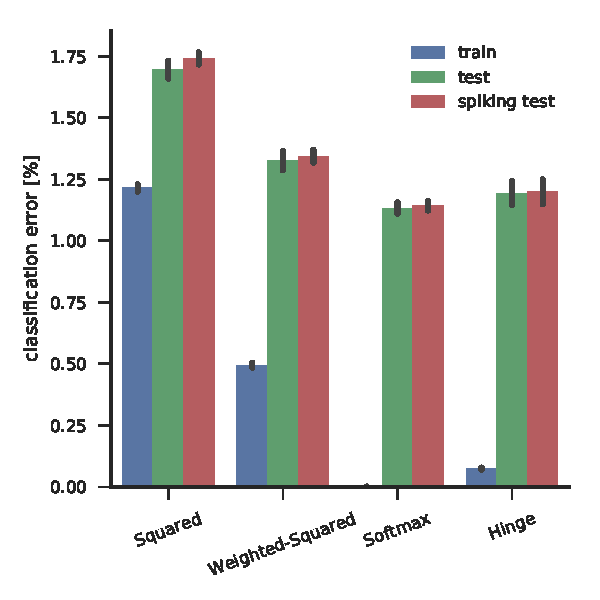
\includegraphics[width=4in]{mnist_compare_decoder_spiking.pdf}
  \captionb{Comparison of loss functions for spiking networks.}{
    The train, test, and spiking classification errors for each loss function
    using 5000 Gabor-encoder neurons on the MNIST task.
    Error bars show 95\% confidence intervals of the mean over 10 trials.
    On average, softmax loss performs the best,
    though it is not statistically much different than hinge loss.
  }
  \figlabel{nef-spikingdecoders}
\end{figure}

\fig{nef-spikingdecoders} shows the best results (optimal $\rho$)
for each loss function.
Softmax loss performs the best, both on the training and test sets,
and in spiking neurons, with hinge loss a close second.
Furthermore, the implicit and explicit margins enforced by
softmax and hinge loss, respectively,
help them both to generalize to spiking neurons very well.
By contrast, unweighted squared loss makes a number more errors
when using spiking neurons,
even with the optimal amount of regularization as shown in the figure.

I chose the spike rates of the network to be low enough
that they are both on the same order of magnitude as cortical spike rates,
and to allow them to be implemented on neuromorphic hardware.
Furthermore, low spike rates also help demonstrate that the network
is truly robust to the variability caused by spikes;
neurons with high spike rates, when filtered by a synapse,
end up having very low variability in their output,
and act essentially as rate neurons.
The neurons in the spiking networks presented here all had
average neuron firing rates between 17 and 19 Hz.
The firing was somewhat sparse, with an average of 30-32\% of neurons
responding to any particular input.
Thus, the average firing rate of neurons when they are responding is higher,
in the 58-60 Hz range.


\subsection{Computation time}

\begin{figure}
  \centering
  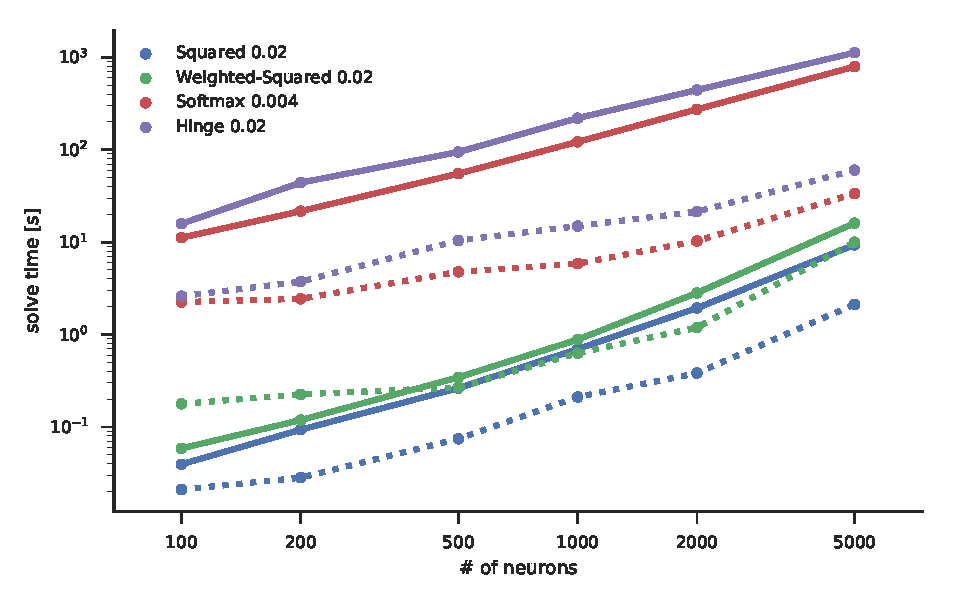
\includegraphics[width=6.35in]{mnist_compare_solve_time.pdf}
  \captionb{Training time for the various loss functions.}{
    Solid lines show CPU times, dotted lines show GPU times.
    CPU: OpenBLAS on Intel Xeon E5-1650 @ 3.5GHz (6 cores),
    GPU: clBLAS on NVIDIA GTX 980 @ 1126 MHz (2048 cores)
    %% GPU: clBLAS on NVIDIA GTX 980 @ 4.6 TFLOPs
  }
  \figlabel{nef-solvetime}
\end{figure}

\fig{nef-solvetime} shows the time required for training
for various loss functions on both CPU (solid line) and GPU (dotted line).
Both axes are logarithmic,
so the slope of the line indicates how the computation speed scales
with the number of neurons,
with a slope of unity corresponding to linear scaling.

The solvers can be grouped into two categories:
the squared loss solvers, which both use direct solution methods;
and the softmax and hinge loss solvers, which use iterative solution methods.
Given the number of training examples $M$ (60000 for the MNIST dataset used here),
the number of neurons $N$,
and the number of categories $C$ (10 for MNIST),
we can compute order of magnitude
of the theoretical computational complexity for each method.
The direct methods both involve computing a correlation matrix
between all the neurons over all the examples,
which is $O(MN^2)$.
The $N$-dimensional linear system corresponding to this matrix
then has to be solved; this is $O(N^3)$.
These are the two main steps in both the squared loss algorithms.
All the other steps in these algorithms are of lower orders (\eg/ $O(N^2)$).
The order of the squared loss algorithm is thus $O(MN^2 + N^3)$.
Since the weighted squared loss requires solving
a separate system for each output category,
its order is $O(CMN^2 + CN^3)$.
Using the method described in \app{wlls},
this can be reduced to $O(2MN^2 + CN^3)$.
Since it is often the case that $M \gg N$,
these methods are often dominated by the $O(MN^2)$ term;
that is, the matrix-matrix multiply is the most costly operation.
This means that as we vary $N$, we expect the solvers to vary as $N^2$.

In \fig{nef-solvetime},
we see that the squared solvers actually vary as somewhere
between $N$ and $N^2$ on the CPU (solid blue and green lines).
This is likely because as the size of the computation grows,
overhead costs become less significant,
and computations can be performed at closer to optimal speed.
A detailed examination of the plot shows that as $N \to 5000$,
the slope of both lines approaches $N^2$.
The weighted squared solver is consistently slightly slower
than the squared solver,
as one would expect from the analysis above.
This effect becomes slightly more pronounced as $N$ increases,
because as $N \to 5000$, $CN \to M$,
which means that the $O(CN^3)$ term begins to compete with the $O(2MN^2)$ term.
I expect this speed difference to become more pronounced as $N$ continues to increase.

A theoretical analysis for the softmax and hinge loss algorithms
is more difficult to perform,
because these algorithms have one important unknown:
the number of iterations required for convergence.
The main factor that affects the number of iterations
is the conditioning of the problem,
where better-conditioned problems will converge more quickly.
Thus, the amount of regularization can have a significant effect
on the convergence;
here, I used the optimal regularization as determined previously,
since this seemed like the most pertinent choice.
What we can do is compute the computational complexity
of the cost and gradient computations that happen each iteration.
For both algorithms,
the computational complexity of a cost-gradient computation
is dominated by two matrix-matrix products,
one between the neuron activities and the parameters to determine the outputs,
and the second between the neuron activities and the output derivatives
to determine the parameter gradients.
Both of these operations are $O(MNC)$,
making the cost of one step $O(2MNC)$.
Thus, assuming the number of required iterations
is independent of the number of neurons,
both these algorithms should scale linearly with the number of neurons $N$.

Looking at the time taken on the CPU by softmax (red solid line)
and hinge loss (purple solid line) in \fig{nef-solvetime},
these two functions do appear to scale almost linearly
with the number of neurons
(a careful examination reveals that they are slightly supralinear).
Hinge loss consistently takes more time than softmax loss;
this appears to be because hinge loss often runs for more iterations
than softmax loss.

All of these solution methods are at least partially parallelizable.
All the matrix-matrix products can be parallelized,
reducing some of the most costly operations for all algorithms.
The only costly operation that I have not parallelized here
is the solution of the linear system(s) in the direct methods.\footnote{
  Parallel algorithms do exist for Cholesky factorization,
  and have been implemented in OpenCL
  (see \url{http://icl.cs.utk.edu/magma/software/view.html?id=190}).
  However, this code has not been ported to work with PyOpenCL,
  as far as I am aware.
  Doing so would not be difficult,
  but since solving the linear systems is typically the less costly part
  of the algorithms explored here,
  I did not take the time to do so myself.}
As \fig{nef-solvetime} shows,
running these algorithms on the GPU is almost always faster than on the CPU,
with the exception being the weighted squared loss for smaller number of neurons.
Overall, weighted squared loss receives the least benefit from the GPU,
since it relies most heavily on solving linear systems,
which I am not running on the GPU.
A close examination shows that for larger number of neurons,
the scaling with $N$ is the same on the GPU as on the CPU.
This is as expected, since larger $N$ are able to utilize all GPU cores,
thus increasing $N$ past that threshold will scale the computation time
as per the theoretical analysis.

\begin{table}
  \centering
  \begin{tabular}{lrrr}
    Core method           & Single $\rho$ & Many (30) $\rho$ & LOO method \\\hline
    Squared loss          & 16.07 s       & 482.10 s         & 81.97 s \\
    Weighted squared loss & 25.63 s       & 768.90 s         & 1054.06 s \\
  \end{tabular}
  \captionb{Computation time of the LOO cross-validation method.}{
    As compared with brute-force validation on a separate validation set.
    The first column shows the cost of running either method for a single
    value of the regularization parameter $\rho$, for 5000 neurons.
    The second column shows the cost of running the single method 30 times,
    which would be the approximate cost of doing cross validation
    on a separate validation set by grid search.
    The third column shows the cost of the LOO method.
    For unweighted squared loss, the LOO method offers potential savings,
    but it performs worse on the weighted squared loss.
    }
  \tablabel{rifkin}
\end{table}

\tab{rifkin} shows the results of testing the computation time
of the \textcite{Rifkin2007} method
for finding the optimal regularization parameter using the LOO error.
When using squared loss, the cost of the LOO method is roughly five times
that of the basic method.
This additional cost is mainly due to computing $\mat P = \mat A \mat Q$,
which is an $O(MN^2)$ operation like $\mat A \mat A^T$,
but unlike the computation of $\mat A \mat A^T$,
the result is not symmetric, so it requires twice the computation time.
The remaining computational costs are due largely to the matrix-vector
products required for testing each different value of $\rho$.
Despite this large increase in computation time,
the LOO method is still more computationally efficient than
running the basic method 30 times to test sufficient values of $\rho$
to get a decent estimate using a separate validation set.
If instead of using grid search to perform the cross-validation
on a separate validation set,
we used an optimization method such as golden-section search,
roughly 15 test values of $\rho$ would be required instead of 30
(based on observations from testing the LOO cross-validation).
This would cut the times of the middle column in half,
though for unweighted squared error, the LOO method would still perform better.

For weighted squared error, the LOO method is much more costly.
This is because we now require $C$ additional matrix-matrix products of $O(MN^2)$,
in addition to the other computations required for computing the LOO error.
This results in the LOO method being sub-optimal for weighted squared error,
taking more time than a brute-force grid-search cross-validation
on a separate validation set.


\section{Discussion}

Of the encoder generation methods examined in \scn{enc-results},
Gabor filters perform best (\fig{nef-encoder-summary}).
This is in spite of the fact that they are tuned for general image statistics,
whereas the encoders yielded by the CIW and CD methods
are tuned for the specific dataset (MNIST, in this case).
This suggests that tuning encoders to each specific dataset is not necessary,
at least for the first layer of hidden neurons.
While using Gabor filters for encoding is not a new idea,
the fact that they perform better than the newer CIW and CD methods
suggests that the utility of these new methods is limited
in terms of generating first-layer encoders.

\fig{nef-decoders} shows that unweighted squared loss performs worst
of all the loss functions examined.
Since it is still the norm
for many recent fixed-encoder networks \parencite[\eg/][]{McDonnell2015},
these results suggest better loss functions could considerably improve
current state-of-the-art results.
Weighted squared loss is computable for a relatively small cost
over unweighted squared loss (see \app{wlls}),
and even softmax loss or hinge loss minimization can be performed
in a very reasonable amount of time on a GPU (\fig{nef-solvetime}).

Softmax loss appears to be the overall best loss function
for fixed-encoding SLFNs for MNIST.
Not only does it yield the best results
(though hinge loss is not significantly worse, see \fig{nef-spikingdecoders}),
it is also the least sensitive to the amount of regularization
(Figures \figref{nef-regularization} and \figref{nef-spikingregularization}).
The main downside to softmax loss is that
it requires more computation time than squared loss methods
(\fig{nef-solvetime}),
since a closed-form solution is not possible.

All of the loss functions presented in this chapter
can theoretically be used with the Prescribed Error Sensitivity (PES)
learning rule \parencite{MacNeil2011,Bekolay2013},
a derivative-free variant of the delta rule adapted for NEF networks.
This would allow decoders to be learned online in a biologically-plausible manner.
Some loss functions might be more amenable to this than others.
For example, the squared loss has a linear derivative,
and is the standard for both online and offline learning in NEF networks.
The weighted squared loss also has a linear derivative,
but the weighting terms will require scaling the learning on different decoders
depending on the target class of the digit.
The softmax and hinge loss both have nonlinear derivatives.
The softmax loss requires computing a softmax function,
which requires normalization and may not be straightforward in spiking neurons.
Hinge loss requires computing an argmax function,
which again is not straightforward,
though there is evidence for such functions being computed
in specialized regions such as the basal ganglia \parencite{Redgrave1999}.

There is a significant drawback to the methods examined in this chapter:
they may not be able to generalize to more difficult datasets,
and even if they can, they may require so many hidden neurons to perform well
that training them becomes infeasible.
So far, fixed-encoding networks have predominantly been tested
on the MNIST dataset.
This dataset does not have the complexity of other,
more realistic datasets like CIFAR-10.
The visual appearance of MNIST digits is very simple,
with trivially distinguishable foreground and background.
The categories are also very distinguishable,
depending on only a few simple visual features.

For more complex datasets,
it is unlikely that SLFNs will be able to perform well.
I tried the networks described in this chapter on the CIFAR-10 dataset,
using 15000 hidden units as well as data augmentation,
and achieved 36\% test error (27\% train error),
which is nowhere near the state-of-the-art.
The best performance for fixed-encoding networks on the CIFAR-10 dataset
is by \textcite{McDonnell2015a},
who use a two-layer fixed-encoding network
with a 96-filter convolution and pooling layer
followed by a 40000 hidden unit fully-connected layer,
to achieve 24.14\% test error.
An identical network achieves 3.96\% test error on the SVHN dataset.
Multilayer networks, particularly those with convolution and pooling,
make solving problems like translation invariance
much more straightforward than with a single-layer network.
The convolutional filters in this network are taken from the Overfeat
network trained on ImageNet,
thus incorporating significant prior knowledge about what constitutes good
low level features.
Yet even this large fixed-encoding network
using good convolutional features and pooling
is still a ways from the state-of-the-art,
having about twice the level of error on SVHN (3.96\% vs 1.92\%)
and 2.5 times the level of error on CIFAR-10 (24.14\% vs 9.78\%)
as compared with the best networks trained on these datasets
(without data augmentation).
These are significant gaps,
and it is unclear whether fixed-encoding networks
will be able to overcome them.\footnote{
  The only way that I currently think that fixed-encoding networks
  might do well on these more challenging problems
  is by training a deep network on an even more difficult problem (\eg/ ImageNet),
  and then replacing the final (classifier) layer on the deep network
  with a classifier trained using one of the methods discussed in this chapter.
  In other words, using the whole deep network as the fixed encoder.
  In my opinion, this would not demonstrate
  the power of fixed-encoding networks
  (since one has to train a deep network on a much harder dataset first),
  but would rather demonstrate that transfer learning is viable.}


% NEF method cannot work well for some architectures. For example, a
% 30-20-10 network trying to learn a linear transform. Even if the encoders
% map the input data distribution, the optimal encoders also depend on the
% output function distribution, \ie/ there are degrees of freedom in the input
% that do not affect the output.

On a deeper level,
there are limitations to what types of processing a fixed-encoding network
can hope to perform,
even with a data-driven encoding.
For example, take the problem of learning a linear transform $\mat B$
from $m$ dimensions to $n$ dimensions, where $m \gg n$.
Because the input space is so much larger than the output space,
there will be dimensions of the input space that do not affect the output;
we call these invariances,
and mathematically they correspond to the nullspace of $\mat B$.
If we create a network that uses some sort of random encoding of the input space,
or even learns some encoding using unsupervised learning,
the best we can hope to do is to perfectly represent the input space,
ideally in some way that is sparser or otherwise easier to work with
than the inputs themselves.
We can never hope, though,
that this encoding will pick up on any of the invariances in the dataset.
That is because these invariances depend on the transformation $\mat B$,
and without some explicit or implicit knowledge about this transformation,
we cannot hope to learn them.
It may be possible to take advantage of prior or expert knowledge
about the domain to engineer better features;
this would be using explicit knowledge of $\mat B$.
Or we may have access to some of the mappings
from the input space to the output space,
and can use them in a supervised or semi-supervised learning setting;
this would be using implicit knowledge about $\mat B$.
%% If the encoding is simply concerned with representing the input image

% Lighting invariance
An example of real-world invariance is lighting.
The lighting on a scene can greatly affect the image that falls on one's retina,
but does not affect the identity of the objects in the scene.
For the most part, we are able to operate accurately in scenes lit in many different ways.
Human object recognition must therefore be invariant to many types of lighting variation.
For a computational visual system to be successful,
it must also be able to separate lighting variation from other object characteristics
in such a way that object recognition can be lighting invariant.
Since our fixed-encoding network cannot learn this implicitly
from the training data using supervised learning,
this invariance must be engineered in.
Specifically, we must engineer the system
such that the effects of lighting are factored out,
having some hidden nodes that represent lighting
and some that represent other image features.
Explicitly constructing such a system is no mean feat, however,
and some of the best successes so far have come from using
unsupervised methods to learn this decomposition \parencite{Tang2012}.

For fixed-encoding networks to truly be successful, then,
the designers of such networks will explicitly have to build in invariances
such that the classifier at the end of the network
is able to easily separate the different classes.
The convolutional-pooling fixed-encoding networks of \textcite{McDonnell2015a}
are another example of building in such an invariance,
in that case an invariance to translation.
In this chapter, I used explicit knowledge of the image space---%
namely the fact that natural images are well-modeled by Gabor filters---%
to design a fixed-encoding network.
In its own way, this is building invariance into the network:
invariance to individual pixel fluctuations.
I used the prior knowledge that individual pixel values do not matter by themselves,
but it is rather the edges in an image, or the correlations between many adjacent pixels,
that matter.
However, that invariance will not be enough by itself,
and for that matter, neither will building in only lighting invariances
or only translation invariances.
A good object recognition system will have to account for all these invariances,
and under a fixed-encoding system,
it will be up to the system engineers to enumerate them and build them all in.

These challenges are severe,
and are one of the reasons that the computer vision community
has slowly been moving away from traditional computer vision,
where features are hand-engineered,
and tending towards machine learning approaches,
where the features are discovered using supervised learning approaches.
Such approaches are the focus of the next two chapters of this thesis.

%%  LocalWords:  nef feedforward SLFNs MLP Pao Eliasmith Broomhead ij
%%  LocalWords:  SLFN ik kj ELMs Tapson Zhu Toh lifrate gabor gabors
%%  LocalWords:  RFs CIW ki squaredloss lstsq Rosasco wsquaredloss un
%%  LocalWords:  Fieguth wsquare wlls softmaxloss BFGS Liu Scipy ka
%%  LocalWords:  hingeloss dec Rifkin rifkin eigen jj MNC CMN Spaun
%%  LocalWords:  Cao Diehl Bekolay spikingregularization OpenBLAS GTX
%%  LocalWords:  spikingdecoders Xeon clBLAS solvetime CN lrrr SVHN
%%  LocalWords:  Overfeat RBF Olshausen Krizhevsky PES MacNeil
%%  LocalWords:  argmax

\chapter{Spiking Deep Networks}
\chplabel{spike}

%% This chapter of my thesis details how
%% I implemented a deep convolutional neural network
%% using spiking LIF neurons.
%% I will begin by introducing and motivating the problem,
%% and provide background on previous work in the area.

At the end of the previous chapter,
we saw that fixed-encoding networks can be used to construct spiking networks
that perform well on smaller datasets.
However, that method does not generalize well to larger datasets.
Deep artificial neural networks have been used by the machine learning field
to perform object recognition on very large, challenging datasets \parencite{Krizhevsky2012}.
How to construct and train such networks in rate neurons
is a relatively well-studied problem;
how the same types of networks might be constructed and trained
with spiking neurons, less so.
This chapter describes a novel implementation of
a deep convolutional neural network using spiking LIF neurons.
Some of this work has been previously described in
\textcite{Hunsberger2015} and \textcite{Hunsberger2016},
and has been expanded on for this thesis.


\section{Background}

Deep artificial neural networks (DNNs),
specifically convolutional neural networks (CNNs, see \scn{cnns}),
are one of the success stories of modern computer vision.
They have been able to successfully recognize a wide range of objects
in large, complex images \parencite[\eg/][]{Krizhevsky2012}.
However, these networks have all been designed for and run using rate-based neurons.
The question of how they can be run in spiking neurons
is an expanding area of research.

Why would we want to run such networks in spiking neurons?
There are two main motivations behind making deep spiking networks.
The first is to allow some of the large CNN models
that have recently had success at numerous object recognition and other tasks
to run on spiking neuromorphic hardware.
This will open the door for energy-efficient systems
performing object recognition in real time on robotic platforms,
where current technology is too energy-intensive
to allow for deployment on mobile robots, for example.

The second motivation is to bring more brain-like components
into machine learning models.
There are many unique challenges related to learning in the brain,
such as how to deal with the nonlinear nature of neurons,
particularly around their firing thresholds,
and how to deal with the discreteness and variability that comes with
communicating using spikes.
While the spiking deep networks introduced here
are not intended to be models of how the brain learns
(the learning procedure is not neurally plausible),
the challenges addressed in this chapter are also faced by the brain,
and some of the ideas in this part help motivate
the more biologically plausible learning mechanisms proposed
in \chp{learning}.

%% Compared with traditional ANNs, which use real-valued nonlinearities,
%% spiking nonlinearities provide a number of challenges to training the network:
%% \begin{enumerate}
%%   \item Non-differentiability of the nonlinearity
%%   \item Increased variability in the output of the nonlinearity for a fixed input
%%   \item An added dimension of time, resulting in dynamics not observed in traditional ANNs.
%% \end{enumerate}
%% These challenges can and have been addressed in many different ways,
%% with the approaches divisible into two main categories:
%% rate-based methods,
%% which use a firing-rate approximation of the spiking neural process for training;
%% spike-based methods,
%% which typically optimize the spike times of the neurons.

% Differences:
%  - spiking neurons have time
%  - spikes are discrete, and if we look at a time bin the rate is discrete
%  - spiking signal is more ``variable''
Spiking deep networks transmit information between neurons
in the form of discrete spikes.
The first difference to notice about spiking networks is that there
is an added dimension of time not typically present in rate-based DNNs.
That is, a spiking neuron is a process that evolves over time,
sometimes emitting spikes, sometimes not.
It only makes sense to talk about this process over time;
looking at it in one instant tells us little about what is going on.
%% If we discretize time (as is common in numerical simulations of neural processes),
%% then a neuron is either spiking in a time bin, or it is not.
In rate-based networks, on the other hand,
we typically present an input and can instantaneously determine the activities
of each subsequent neuron in the network,
since they do not change over time.

The second difference to notice is that spikes are discrete
and all identical.
The only information that a spike carries is the time at which it occurred.
As discussed in \scn{codes}, this means that there are two main types of codes
a neuron can use: rate codes, or timing codes.
If we use a timing code, then we are concerned about the times of individual spikes.
If we use a rate code, then we are more concerned about the number of spikes
in a particular time window,
or perhaps the relative timing of spikes with respect to one another.
When looking at the number of spikes in a time window,
we are faced with the additional challenge that the resulting rate is discrete.
If there are $n$ spikes in the $t$ second window,
then the firing rate is $n / t$, where $n$ is an integer.
For a fixed window $t$, there are only a discrete number of values that
this firing rate can take on,
specifically all the integer values of $n$.

The third difference to notice is that the output of spiking neurons is
inherently more variable than their rate-based counterparts.
Given a constant input, a rate neuron will give a constant output,
that is, the firing rate corresponding to that input.\footnote{
  Rate neurons can have internal dynamics
  (\eg/ the adapting version of the rate-based LIF),
  and given a constant input, the output of these neurons will not be constant.
  However, their output is still much less variable
  than their spiking counterparts.}
Spiking neurons, on the other hand, will output a spike train,
which when filtered by a synapse,
results in an oscillating signal
whose variability depends on the firing rate.
Thus, even when presented with a constant input,
a spiking network will show variability in the inputs to each neuron,
and the outputs of the entire network.

DNNs are traditionally rate-based,
in that the nonlinearity activity implicitly represents the firing rate of a neuron.
For example, a ReLU can be viewed as a neuron that is silent if its input is below zero,
and whose firing rate increases linearly as the current increases above zero.
Furthermore, rate-based DNNs have cost functions that are based on
the activities (firing rates) of the output neurons:
if the network is performing classification,
the chosen class is the output unit with the highest activity.
One approach is therefore to treat spiking networks similarly,
and train the network so that the unit corresponding to the target class
will have the highest activity.\footnote{
  This activity does not necessarily correspond to a neuron firing rate.
  In fact, it is more likely the filtered, weighted sum over the spiking activities
  of the final layer of neurons in the network.}
The alternative is to train the network so that the first neuron to spike
will be the chosen class.

At the level of a single neuron, this distinction goes away.
The activity of a neuron firing at a regular rate
is captured by its inter-spike interval,
the time between one spike and the next.
Assuming the neuron starts in a resting state,
the inter-spike interval is equivalent
to the time before the first spike of a neuron (plus the refractory period).
The key design decision is how we transmit information between neurons.
\emph{Spike-based optimization methods}
compute the exact spike times of neurons,
and use these to compute the spike times of neurons in subsequent layers.
\emph{Rate-based optimization methods}, on the other hand,
treat neurons as idealized rate-response curves,
and only transmit firing \emph{rates} within the network.

%% The key challenge faced by spiking networks
%% is that there is no clear way to take the derivative of a spiking neuron
%% with respect to its input.
%% The first part of this problem is that it is not even clear
%% what we should take the derivative \emph{of}:
%% should we take the derivative of the firing \emph{rate} of the neuron \wrt/ the input,
%% or should we take the derivative of the first spike \emph{time}?
%% Essentially, this is the question of which metric to use,
%% except here we are talking about a single neuron within the network,
%% not the network output.
%% %% The second part of this problem is that for either choice of metric,
%% %% there is no clear way to take the derivative of the spiking neuron.
%% If we choose the activity metric,
%% then there is no clear way to take the derivative of the spiking neuron.
%% The firing rate of a neuron over a period is a discrete value,
%% since the number of spikes in the interval must be an integer.
%% This means that the derivative is essentially infinite if an infinitesimal
%% change in the input would change the number of output spikes in the interval,
%% and zero otherwise; thus, the derivative is undefined.
%% This is the main challenge faced by \emph{rate-based optimization methods}.
%% If we choose the first-to-spike metric,
%% the procedure for taking the derivative is more clear:
%% if the neuron is currently firing at least one spike,
%% then the derivative is based on how much a change in the input
%% changes the time of that first spike,
%% and if the neuron is not firing a spike,
%% then the derivative is zero
%% (the details vary between implementations).
%% This is the basis for \emph{spike-based optimization methods}.

%% While rate-based and spike-based optimization methods
%% are optimizing different metrics,
%% there is a connection between the activity metric and the first-to-spike metric.
%% Namely, a neuron that spikes more quickly does so because it has stronger inputs,
%% which would also lead to increased activity.
%% It is therefore likely that the networks resulting from these
%% two different optimization methods are quite similar.
%% Their main difference should only be seen
%% when all neural and synaptic activities are starting at zero;
%% in this situation, the first-to-spike metric can better account
%% for the precise timing of spikes and potentially result
%% in a faster decision.
%% Not surprisingly, all the networks I am aware of
%% that use spike-based optimization methods
%% do reset the system between stimulus presentations.
%% Once the networks have been running (for example when using continuous inputs),
%% I expect the two types of networks to perform similarly.
%% However, I am not aware of any such comparison in the literature.


\subsection{Spike-based optimization methods}
\scnlabel{spikingmethods}

Spike-based methods optimize the times of individual neuron spikes
to reduce the overall error of the network.
Because the time at which a neuron spikes is a continuous value,
continuous optimization methods can be used.
However, the problem is still highly nonlinear,
because a small change in the input to a neuron
(and thus a small change to the neuron's input weights)
can push a neuron over its firing threshold,
eliciting a spike and drastically changing the output of the neuron \parencite{Gutig2014}.

%% Typically just care about first spike time, but some relaxing this (Stromatias2014)


%% SpikeProp (Bohte 2000)
The first algorithm to perform supervised deep learning
by optimizing spike times was SpikeProp \parencite{Bohte2002}.
This algorithm makes the simplifying assumption that
each neuron fires at most one spike during the spiking interval,
or if multiple spikes are fired,
only the first is optimized.
It also has the structural qualification that each connection
is composed of many different synaptic terminals,
each with a different synaptic delay and a different connection weight.
They demonstrate that their algorithm can solve the XOR problem,
and performs comparably to backpropagation optimized both
with gradient descent (GD) and Levenberg-Marquardt (LM)
on a number of small datasets
(the largest having 36 input dimensions, six output classes, and 4435 training examples).
The single-spike optimization procedure and multiple connection weights per synapse
have made it difficult to expand this work to larger datasets.
\textcite{McKennoch2006} present two methods to improve
the rate of convergence of SpikeProp,
though the applications are still limited to small datasets.

%% Mostafa2016:
\textcite{Mostafa2016} proposes an alternative to the SpikeProp algorithm,
designed specifically for non-leaky integrate-and-fire neurons.
It relaxes the restriction that a connection must be composed of
many different discrete-delay elements,
and instead uses a more standard network architecture,
with one exponential-synapse connection between each pair of neurons.
They train networks with both one and two hidden layers,
achieving 2.45\% and 2.86\% on MNIST, respectively.
One challenge the author faced was that dropout,
the most common regularization technique,
did not work in the network in question
because it would often prevent neurons from firing at all.
Lacking a good alternative regularization method,
the networks suffered from large generalization errors
(the training error for both networks was almost zero).

%% Stromatias2014: using GA to optimize spike times (allows more than one spike per neuron)
Whereas the previous algorithms only optimize the first spike of each neuron,
\textcite{Stromatias2014} relax this restriction.
They use a genetic algorithm to optimize multiple spikes from each neuron.
However, they only demonstrate their algorithm
on relatively small models with fewer than 10 hidden neurons.
Genetic algorithms often have problems scaling
to problems with many parameters,
thus this algorithm may have trouble scaling to datasets like MNIST or CIFAR-10.

%% Friedeman Zenke (Cosyne DL workshop)

%% Robert Gütig (Cosyne DL workshop)

% --- continuous time methods
% Lee et al (2016) Training Deep Spiking Neural Networks using Backpropagation
% - this is specific to LIF neurons, would not work for adapting (also, deals
%   only with first spike, so definitely not for adapting)

\textcite{Lee2016} also optimize over multiple spikes per neuron.
They ignore the spiking discontinuity during backpropagation,
and treat the output of a neuron as a linear function of its inputs
(where the inputs have been filtered by the membrane of the neuron in question).
This allows them to run the network in spiking neurons during training,
but still perform backpropagation without worrying about discontinuities.
They also ignore the refractory period of the neurons,
stating that it is short compared to the time between spikes
and thus has little effect on firing rates.
They add lateral inhibition components to increase network performance,
but only optimize over the first-order derivatives caused by these connections.
Despite these simplifications,
their method is still able to learn appropriately on the MNIST task,
achieving 1.30\% error using standard SGD
and 1.23\% error using an ADAM optimizer.
While it remains to be seen whether this method
can generalize to larger datasets in a tractable way,
it introduces a number of new ideas for training spiking networks
that will hopefully be improved upon by future work.

\textcite{Huh2017} introduce a novel method
to make the spiking process continuous.
They introduce a gating function $g(V)$ of the membrane voltage $V$
that is greater than zero for voltages near the firing threshold,
and zero otherwise, with unit integral.
They call the region where $g(V) > 0$ the \emph{active zone}.
Rather than having efferent synapses receive a current $\delta(t - t_k)$
when the neuron spikes (crosses the firing threshold) at time $t_k$,
synapses continuously receive current based on $g(V) \diff{V}{t}$.
If the voltage is outside the active zone, this term is zero because $g(V) = 0$.
If the voltage crosses the active zone (and thus the neuron spikes)
the integral of this term is one.
Finally, if the voltage enters the active zone,
but does not cross its upper threshold (\ie/ the firing threshold),
then the integral of the term will be a positive number between zero and one
(this is something akin to a partial spike).
This induced synaptic current is almost identical
to the traditional spiking current $\delta(t - t_k)$ in the extremes
(\ie/ when the neuron is silent or firing reasonably quickly),
but continuous in the middle region.
The authors can then achieve a gradient through the network
at any particular point in time using backpropagation,
and optimize the entire network using backpropagation through time.
Their results focus on tasks that require dynamic, temporal representation,
such as predictive coding.
This is a different focus than most other spike-based methods,
which typically focus on static tasks (\ie/ object classification),
and thus a direct comparison is difficult.
Because the method makes the neural nonlinearity differentiable,
it allows the use of many different neuron models:
the paper uses non-leaky integrate-and-fire and
quadratic integrate-and-fire,
and others would certainly be compatible.
This, along with the ability to optimize recurrent spiking networks well,
make this a potentially powerful method for dynamic spiking networks.
For networks focused on static tasks,
I believe that the requirement of this method to optimize over
potentially long time series for each input stimulus
would make it ill-suited for training large object classification networks.

To date, spike-based optimization methods have not been applied
to larger, deeper architectures like CNNs.
This has prevented spike-based training on any datasets
larger or more challenging than MNIST.
Part of the challenge is simply computational:
spike-based optimization methods require more computational resources
than rate-based methods,
since the network is dynamic and requires iterative simulation
for each stimulus presentation.
Most of the current software has been designed for static ANNs,
and expanding it to spiking networks is non-trivial.
%% The other part of the challenge is that convolutional networks use tied weights.
%% While most spike-based algorithms do generate a gradient,
%% and the gradient for a tied weight is simply the sum of the individual gradients
%% across the equivalent untied components,
%% it is not yet tested how well this will work in spiking networks,
%% since it will limit the control over
%% For these reasons,
For this reason,
researchers have turned to rate-based optimization methods
to tackle larger datasets with spiking networks;
this is the focus of the next section.


\subsection{Rate-based optimization methods}
\scnlabel{ratemethods}

Rate-based optimization methods make the simplifying assumption
that all neurons are performing rate coding (see \scn{codes}).
Therefore, these methods do not care about the times of individual spikes,
only the number of spikes over a time period.
Almost always, these types of methods use this simplifying assumption
to replace the spiking neural process with a continuous-valued rate approximation.
For derivative-based methods, this rate approximation is then differentiated.
Derivative-free methods, on the other hand, avoid taking the derivative
of this rate approximation,
and instead opt for an optimization method such as Contrastive Divergence
that does not require it.
Finally, function approximation methods approach the problem differently:
rather than assuming a network of spiking neurons and trying to find
rate approximations to these spiking neurons,
they choose an arbitrary nonlinearity for training the network,
and then use spiking neurons to approximate this nonlinearity.


\subsubsection{Derivative-based methods}

\textcite{Perez-Carrasco2010} describe the first work to train a spiking convolutional network.
%% and one of the first examples of a
They trained a traditional CNN with tanh units using backpropagation.
To convert this to a spiking network,
they replaced the tanh units with binary threshold units
with a refractory period.
Specifically, if the input to a neuron is above a certain threshold,
it fires a spike,
after which the neuron cannot spike for a set period.
This refractory period causes the firing rates of the neurons to saturate.
The authors argue that this helps to ``emulate the corresponding sigmoid functions''
(that is, the tanh function) used in the rate model.
They do not explain exactly how the refractory period does this.
Presumably, they mean because the tanh function is a saturating nonlinearity,
having the neuron firing rate saturate makes the firing rate curve
more similar to the tanh curve.

%% then converted this to a spiking network by approximating the tanh units
%% with IF units with refractory period.
%% The refractory period causes the spike rate to saturate,
%% allowing the unit to better fit the tanh curve.

\textcite{Cao2014} took a more principled approach to converting
rate-based CNNs to spiking CNNs.
They took advantage of the fact that rectified linear units (ReLUs)
perfectly model the rate of a non-leaky integrate-and-fire neuron (IF).
Since ReLUs are currently the standard for deep networks,
this allows networks to be trained with the same rate-based ReLUs,
and then replaced with spiking IF neurons at runtime.
They also replaced the max-pooling layers used by the network
with average pooling layers.
Average pooling layers only involve summing and scaling the inputs,
allowing them to work well with spiking neurons,
moreover in a biologically plausible manner.
Max pooling, on the other hand, has no clear spiking analogue:
taking the max of the binary spikes coming in at the current point in time
(\ie/ outputting one if any of the inputs are spiking, and zero otherwise)
is not at all equivalent to taking the max across spike \emph{rates},
as performed by traditional CNNs.
Furthermore, even taking the max across spikes is not biologically plausible,
since there is no clear neuron-level mechanism for taking the max
across incoming signals.
\textcite{Cao2014} also removed biases from the network,
since they felt these would be difficult for a spiking network to implement.
However, it is not clear why biases would present a problem for spiking networks,
particularly if targeting neuromorphic hardware (much of which supports biases).
%% and later works have included biases.
One advantage to removing biases is that it presents a slightly cleaner biological explanation,
since the output of each neuron depends only on the inputs from other neurons in the network.

\textcite{Diehl2015} employed a similar method to \textcite{Cao2014},
with the addition of a novel normalization method for weight magnitudes.
One key design decision in spiking networks is the tradeoff between
the firing rates of the neurons
and the amount of time needed by the network to make a decision (integration time).
Higher firing rates allow the network to transmit information more quickly,
resulting in faster responses and higher accuracy,
but also use more energy,
and on some neuromorphic platforms there are maximum allowable firing rates.
Increased integration time allows more information to be collected,
resulting in higher accuracy,
but also leads to slower responses and more spikes per example.
Thus, to achieve a balance between
accuracy, response time, and energy efficiency,
the firing rates and integration time need to be properly tuned.
Because ReLUs---and by extension IF neurons---are scale invariant,
the firing rates of neurons in spiking IF networks can be arbitrarily set.
To change the firing rate of a neuron while maintaining the same network,
an increase in the firing rate of the neuron must be met with
a decrease in all connection weights emanating from that neuron.
\textcite{Diehl2015} presents two techniques to normalize network weights
using these ideas: model-based normalization; and data-based normalization.
Both methods are based around the criterion that we do not want
the input to any neuron in a single timestep to be greater than
the firing threshold of that neuron.
If that were to happen,
it could cause the neuron to need to fire two spikes in the same timestep,
something that is not supported by most neuromorphic hardware.
In other terms,
the goal of the normalization is to ensure the instantaneous firing rates
of all neurons never exceeds the rate of the neuromorphic chip (simulation rate).
Model-based normalization finds the maximum sum of positive input weights
across all neurons in a layer,
and then normalizes all neuron inputs in the layer using this sum.
This ensures that no neuron could receive an input greater than
one (the firing threshold) in a single timestep.
The authors found that this technique can make the weights smaller than necessary,
since the maximum possible input to a neuron is often never encountered in real data,
resulting in longer-than-necessary integration times.
Data-based normalization instead bases the normalization
on the examples in the training data.
It ensures that for any given training example,
no neuron will receive an input greater than one (the firing threshold).
The authors found that data-based normalization
decreased the amount of integration time needed by the network
to achieve the same accuracy,
as compared with an un-normalized network with higher firing threshold.
This paper presented state-of-the-art results for spiking networks
on the MNIST dataset, achieving 0.88\% test-set error.

\textcite{Esser2016} trained deep networks
targeting the IBM TrueNorth neuromorphic chip \parencite{Merolla2014}.
Unlike the other networks described here,
this network uses a simple binary threshold neuron,
which fires a ``spike'' if its input is positive at a given time step,
otherwise it is silent.
This is equivalent to a rate-based binary threshold unit.
Additionally, the network only presents each image for a single timestep
before resetting all neuron voltages and presenting the next image.
These considerations make the network rate-based, rather than spiking.
%% Since this neuron function is not differentiable
%% (the derivative is zero at $x = \infty$ and zero elsewhere),
%% they approximated the derivative with the function $\max(0, 1 - \|x\|)$.
They trained very large networks (8 million neurons)
on a number of tasks (including CIFAR-10 and SVHN).
Their results are state-of-the-art if compared to spiking networks,
but the better comparison is to rate-based networks,
where the only innovation is the use of binary threshold units,
which are not commonly used in deep networks.
The network is able to run on neuromorphic hardware (TrueNorth),
but uses many neurons even for modest datasets like CIFAR-10,
and would be difficult to scale to large datasets like ImageNet.


\subsubsection{Derivative-free methods}

Derivative-free, rate-based optimization methods
use rate approximations for the spiking neural process,
but do not require the derivative of the rate approximation.
All such methods I have found base their work on
using the Contrastive Divergence (CD) algorithm \parencite{Hinton2006a}
to train deep networks of stacked RBMs.

\textcite{OConnor2013} create a spiking network of LIF neurons using RBMs.
For training the network,
they use the Siegert approximation to a noisy spiking LIF neuron
as the rate neuron model.
The Siegert approximation is an equation for the mean firing rate of an LIF neuron
given many input spike trains,
where spikes are Poisson distributed with constant firing rate.
These output rates are then normalized by the maximum firing rate $1/t_\text{ref}$
to generate firing probabilities,
and the hidden units are sampled from a binary distribution based on these probabilities.
Training with this model allows the authors to
model some of the variability caused by using spikes.
%% Surprisingly, when running the spiking network for inference,
%% the authors use the Siegert approximation again to determine firing rates
%% and then
They then substitute spiking LIF neurons for these rate neurons
and run the network using Poisson input trains based on pixel intensities,
achieving 5.91\% error on MNIST.
\textcite{Stromatias2015} extends this work by showing that the method
is robust to reduced weight precision,
achieving lower error (5.06\%) on MNIST
using only 11-bit fixed point weights\footnote{
  The 11-bit weights use 3 bits for the integer component
  and 8 bits for the fractional component.}
running on the SpiNNaker platform.

\textcite{Neftci2013} also develop spiking RBMs using LIF neurons.
Their approach fits the average firing rate of a noisy LIF neuron
to a sigmoid curve,
and then trains using this sigmoid curve.
This limits the choice of parameters for the LIF neuron,
in that they must allow the firing rate to be accurately fit by a sigmoid;
however, it allows the RBMs to be trained with traditional sigmoid activation functions,
making the training simpler and more efficient.
They propose an online variant of CD for spiking networks,
building off of an STDP learning rule.
For each presented training image, there are two phases.
The first occurs immediately when the image is presented,
and updates connections based on the data (stimulus).
Then, after a period of time, the recurrent connections become active,
driving the network towards its reconstruction distribution;
this has an effect similar to Gibbs sampling in the CD algorithm.
During this time, the gating signal on the derivative is flipped,
such that the weights are affected negatively based on the reconstruction.
This forms one complete cycle of the algorithm,
and is repeated on each training image,
for many iterations through the training data;
this has an overall effect similar to CD,
thus the authors call it ``event-based CD''.
Using this method, they achieve 8.1\% test-set error on MNIST in spiking neurons.


\subsubsection{Function approximation methods}

Function approximation methods are significantly different than
the previously introduced methods.
Rather than using one spiking neuron to replace each node in the ANN,
function approximation methods use multiple spiking neurons for each node.
They use these spiking neurons to approximate the nonlinear function
(\eg/ sigmoid function) being computed by the node.

I am only aware of one such use of this method, by \textcite{Eliasmith2012}.
They use three spiking LIF neurons to approximate the sigmoid function
computed by each node.
They choose random parameters for each neuron;
most significantly,
they assign a uniformly-distributed random bias current to each neuron.
This allows each of the three neurons to target a different portion of
the sigmoid curve,
and is in addition to the bias current for the node
which is set when training the network.
Once these random parameters are set,
they solve for a scalar weighting for each neuron
that determines how much it contributes to the sigmoid function.
This is the standard NEF method for function approximation (see \scn{nef}),
but applied on a small pool of neurons to approximate a sigmoid function.

This method allows a spiking network to approximate a rate-based network
in a very general way.
One disadvantage is that it uses many more neurons than nodes in the network,
making it more costly in terms of neural resources
than the methods described above.
Its effectiveness also depends highly on how well the neurons can represent
the node function in the operational domain.
Sigmoid functions are relatively easy to represent with LIF neurons.
ReLUs are much flatter and are not squashing,
meaning that the range of output values that the LIF neurons
need to accurately represent is much larger;
this makes them much less amenable to this method.
%% The choice of parameters


\subsection{Noise}

Transmitting discrete, constant-amplitude spikes
(as done throughout much of the human central nervous system)
is a higher-variance method of information transmission
than simply sending a scalar value (such as a voltage).
When taking a rate-based view of neural activity,
one can view this increased variance as ``noise''
around the firing rate (which is the ``signal'').
The firing rate corresponds to the mean value of a spike train signal.
If we pass a spike train through a low-pass filter,
we can view the result as an estimate of this mean
with some additional time-varying noise around it.
The amount of noise depends on the filter used;
cutting out more of the high frequencies
will result in a better estimate with less noise,
but if the underlying firing rate signal is also time-varying,
then we will cut out its higher frequencies as well.
For a spiking network that is receiving a sequence of images
and outputting a response for each in real-time,
this amounts to a longer response time for each image.

Many rate-based spiking neural networks
do not model the variance caused by spikes.
Of those that do, there are two approaches that have been used.
The first is to model the effects of spike noise on the mean neural firing rates,
and then use these revised mean rates when training the model.
The second approach is to include stochastic elements in the model during training,
so that the probability distribution of the training output rates models,
in some way, the variance caused by the spikes used during testing.

%% O'Connor 2013 accounts for spike noise with Siegert model
An example of this first approach is using the Siegert model
to account for the effects of incoming spikes on the LIF neuron firing rate,
as done by \textcite{OConnor2013}.
This approach assumes that neuron inputs are uncorrelated,
with spikes governed by a Poisson process.
The Siegert model then gives the average firing rate of the LIF neuron,
given the average firing rates of all inputs and their respective connection weights.
One drawback to this approach is that the Siegert equation is complicated:
it contains an integral with no closed form solution,
whose integrand contains both the exponential and error (\textrm{erf}) functions.
Computing this function on a GPU (or even a CPU) would be difficult and time-consuming
compared with the functions normally used in neural networks.
The other drawback of this approach is that it requires computing
two linear functions of the input neuron rates,
one to compute the overall input mean and the other to compute the variance.
This means that it requires twice as many matrix-vector operations
as the same network without the Siegert model.

%% Discrete sampling noise: \eg/ Boltzmann machines
%% Noise in RBMs: Nair and Hinton 2010?
The second approach---adding stochastic elements to model spiking noise---%
has often been used in various types of neural networks,
though not with the intent of running the final model in spiking neurons.
A foundational example is Boltzmann machines,
which use binary sampling on probabilistic units \parencite{Hinton1983}.
This allows units to only communicate binary values with one another,
which shares some similarity with spikes.
However, if one views each unit as wanting to transmit
its underlying firing probability (which is like a firing rate),
then this is a very severe form of noise.
Subsequent work by \parencite{Nair2010} greatly relaxed the amount of noise
by having units use rectified linear activation functions
with Gaussian noise on the neuron input.
%% Having such noise sources in a model essentially regularizes the model
Another example of adding stochasticity to a model
is denoising autoencoders \parencite{Vincent2008},
which add noise to model inputs and then attempt
to reproduce the noise-free version of the input.
Adding noise to model inputs has often been used
to help make models better able to deal with a variety of inputs,
essentially it is a type of data augmentation.\footnote{
  Other forms of data augmentation,
  such as translating, rotating, or deforming images,
  can also be viewed as noise on model inputs,
  albeit a more structured form of noise than Gaussian noise.}
However, adding noise to hidden units---%
whether that be to their inputs or outputs---%
is much less common in nonlinear networks \parencite{Poole2014}.
I could not find any examples of it being used
to model the variability caused by spikes
in order to transfer a rate model into spiking neurons.

% Bishop1995: Training with Noise is Equivalent to Tikhonov Regularization


%%%%%%%%%%%%%%%%%%%%%%%%%%%%%%%%%%%%%%%%%%%%%%%%%%%%%%%%%%%%%%%%%%%%%%%%%%%%%%%%
\section{Implementation}

The previous section outlines the many types of methods available
for training deep spiking networks;
each approach has advantages and disadvantages,
with no clear preferred method.
My goal was to implement a deep spiking network
that could process real-world-sized images
depicting a large variety of object categories.
Ultimately, I wanted something that would be able to
process the ImageNet dataset,
a much larger dataset than any spiking network had previously processed.

The ImageNet dataset has a number of defining characteristics:
the images are quite large ($256 \times 256$),
there are over a million training images,
and they are difficult to categorize.
Because of the size, I needed a method that could quickly process
many large images.
This immediately suggested spike-based optimization methods
would not be a good choice,
since they require running each image for a period of time to generate spikes.
If each image needs to run for 100 timesteps,
this means that such dynamic methods would take 100 times longer
than comparable static methods
(assuming no specialized hardware for accelerating spiking computations).
Additionally, all networks that have been successful on ImageNet
are rate based, and by expanding on these methods
I could make use of existing code for training them.

Within the rate-based methods,
I had a choice between derivative-based and derivative-free methods.
The derivative-free methods that I found were all based on
unsupervised learning techniques,
whereas all networks that are successful on the ImageNet dataset
have been trained in a highly supervised manner.
Finally, I did not pursue function approximation methods in depth
because they require many more neurons than methods that incorporate
the neuron tuning curves directly.
Also, my preliminary investigation into function approximation methods
showed that it is difficult to use spiking LIF neurons to properly
represent a ReLU function,
because ReLUs are non-squashing and thus have a wide range of outputs.

These reasons pushed me to implement a deep spiking network
using a derivative-based rate method,
specifically by training a rate-based ANN with neuron-like nonlinearities,
then converting this to a spiking network.
This required three main steps, which I will describe in detail in this section:
1) modifying the architecture to remove components difficult
to implement in neurons;
2) designing a nonlinearity similar to the LIF neuron, but differentiable;
and 3) adding noise during training to increase robustness to spiking variability.
The trained network is then tested with dynamic, spiking neurons.
Since these neurons output signals (\ie/ spike trains)
rather than static scalar values,
the classification procedure also needs to operate over time (see \scn{nef-spiking-methods}).

I evaluate the system on five different datasets:
MNIST, SVHN, CIFAR-10, CIFAR-100, and ILSVRC-2012 (ImageNet).
The datasets are presented in detail in \scn{datasets}.


\subsection{Architecture and modifications}
\scnlabel{spike-architecture}

I based my architecture off of AlexNet \textcite{Krizhevsky2012}.
This architecture won the ILSVRC-2012 (ImageNet) competition,
and a smaller variant of the network achieved $\sim$11\% error on the CIFAR-10 dataset.
I chose it because it is relatively simple,
with very efficient training code freely available.\footnote{
  \url{https://github.com/akrizhevsky/cuda-convnet2}}
%% The AlexNet architecture, though no longer state of the art,

\begin{table}
  \centering
  \begin{tabular}{cc}
    AlexNet & My model \\\hline\hline
    input, 3 channels, $224 \times 224$ & input, 3 channels, $224 \times 224$ \\\hline
    conv 64, size 11, stride 4, padding 0 & conv 64, size 11, stride 4, padding 0 \\
    \textbf{cross-map norm, size 5} & \\
    \textbf{max} pool, size 3, stride 2 & \textbf{avg} pool, size 3, stride 2 \\\hline
    conv 192, size 5, stride 1, padding 2 & conv 192, size 5, stride 1, padding 2 \\
    \textbf{cross-map norm, size 5} & \\
    \textbf{max} pool, size 3, stride 2 & \textbf{avg} pool, size 3, stride 2 \\\hline
    conv 384, size 3, stride 1, padding 1 & conv 384, size 3, stride 1, padding 1 \\
    conv 256, size 3, stride 1, padding 1 & conv 256, size 3, stride 1, padding 1 \\
    conv 256, size 3, stride 1, padding 1 & conv 256, size 3, stride 1, padding 1 \\
    \textbf{max} pool, size 3, stride 2 & \textbf{avg} pool, size 3, stride 2 \\\hline
    full 4096 & full 4096 \\
    dropout, keep 0.5 & dropout, keep 0.5 \\
    full 4096 & full 4096 \\
    dropout, keep 0.5 & dropout, keep 0.5 \\
    full 1000 & full 1000 \\
    \textbf{softmax} & \textbf{softmax (train only)} \\
  \end{tabular}
  \captionb{Details of the AlexNet architecture and the modified version used here.}{
    This is the architecture used for the ImageNet ILSVRC-2012 dataset.
    Differences are highlighted in bold.
    ``conv $n$'' refers to a convolutional layer with $n$ feature maps,
    where ``size'' specifies the filter size.
    ``cross-map norm'' refers to a cross-map normalization layer,
    where ``size'' is the $s$ parameter of the layer.
    ``max pool'' is a max-pooling layer, and ``avg pool'' is an average pooling layer.
    ``full $n$'' is a fully-connected layer with $n$ output neurons.
    ``dropout'' is a dropout layer,
    where ``keep'' is the fraction of output units to keep.
  }
  \tablabel{architectures}
\end{table}

The network is a CNN,
and makes use of the core components of CNNs outlined in \scn{cnns}.
The details of the original architecture are given in \tab{architectures},
along with my modified architecture.\footnote{
  This is the architecture used for the ImageNet ILSVRC-2012 dataset.
  For the other datasets tested,
  I used simplified versions of the architecture.
  Details of these architectures,
  along with all the code for running them,
  can be found at \url{http://github.com/hunse/cuda-convnet2}.}
The original architecture begins with two \emph{generalized convolutional layers},
where each such layer consists of a convolutional layer,
a normalization layer, and a pooling layer.
These are followed by three convolutional layers,
with one pooling layer at the end.
These convolutional layers do not change the size of the image,
and having three of them allows the network to compute more complex nonlinearities.
These are followed by two fully-connected layers, each with dropout.
Finally, the classifier consists of a fully-connected layer
mapping to the 1000-class output space, with a softmax layer.
Neural nonlinearities always occur after each weight layer,
that is, each convolutional or fully-connected layer.
The only exception is the final layer,
where the softmax nonlinearity takes the place of the neural nonlinearities.
Training is performed using a modified version of the LIF rate response function,
described in \scn{softlif}.
For testing, I then run the network dynamically using spiking LIF neurons.

To facilitate running this architecture with spiking neurons,
I made two main modifications.
The first was to remove the normalization layers.
Though normalization layers take inspiration from biology \textcite{Jarrett2009},
it is not clear how spiking neurons could efficiently and robustly
perform this computation.
This type of computation would likely require lateral connections between neurons,
making the network recurrent, and no longer feedforward.
Recurrent networks are much more difficult to train than feedforward ones,
and would require completely different training methods.
As we will see, the normalization layers are non-essential,
and by removing them I was able to train the spiking network using the same
feedforward methods as used on the original network.

The second modification I made was to replace
the max-pooling layers with average-pooling layers.
Like normalization, the ``max'' function is a nonlinear function
that is difficult to compute using spiking neurons.
Again, one way to implement something similar would be with lateral connections,
but I avoided these for the reasons stated above.
Average-pooling, by comparison,
is easy to compute in spiking neurons, since it is a linear operation.

The final structural modification was to use the final softmax layer
during training only,
thereby avoiding the need to implement a ``softmax'' function using spiking neurons.
However, since the classification method takes the maximum output of the network,
and the ``softmax'' function does not affect the maximum value,
this modification should have no effect on the system output.

\begin{table}
  \centering
  \begin{tabular}{lrrrr}
    Dataset & \# neurons & \# weights & \# synapses & FLOPs \\\hline
    MNIST & 27 088 & 6 318 000 & 11 623 200 & 23 298 576 \\
    SVHN & 27 088 & 6 318 800 & 12 250 400 & 24 552 976 \\
    CIFAR-10 & 49 536 & 2 109 376 & 19 512 576 & 39 120 768 \\
    CIFAR-100 & 49 536 & 2 213 056 & 19 616 256 & 39 328 128 \\
    ILSVRC-2012 & 493 184 & 61 090 496 & 714 188 480 & 1 429 246 976 \\
  \end{tabular}
  \captionb{Size metrics for the networks used on all the different tasks.}{
    The number of parameters in each model is equal to the number of weights
    plus the number of neurons (to account for each neuron's bias).
    For fully-connected or locally-connected layers,
    the number of synapses is equal to the number of weights,
    since each weight corresponds to one connection.
    In convolutional layers, the same weight is used for many neural connections;
    this is why the number of synapses is much greater than the number of weights.
    The floating-point operations (FLOPs) corresponds
    to the number of operations required to run the network
    as an ANN using rectified-linear units.
    This will provide a point of comparison
    for running the networks on neuromorphic hardware,
    examined in \scn{spike-efficiency}.
  }
  \tablabel{network-sizes}
\end{table}

A summary of the sizes of the architectures used for each of the tasks
is given in \tab{network-sizes}.
It also presents the number of floating point operations (FLOPs)
required to process one image using the ANN version of the network.
The network used for the ImageNet ILSVRC-2012 task
has ten times more neurons and parameters
and takes 36 times as many FLOPs per image
as any of the other networks.
%% An e


\subsection{The soft-LIF rate neuron}
\scnlabel{softlif}

As described in \scn{ratemethods},
a number of previous works have run deep spiking neuron models
using non-leaky integrate-and-fire (IF) models
without any refractory period between spikes.
This model is particularly amenable to use in spiking deep networks
because its rate response function
is equivalent to the rectified linear unit (ReLU) function
that has become ubiquitous in deep networks.

In my model, I use a \emph{leaky} integrate-and-fire (LIF) neuron model
with a refractory period between spikes.
This not only adds biological realism,
but the refractory period limits the maximum firing rate of the neurons,
potentially reducing their average firing rates as well
and thereby making the networks more efficient on neuromorphic hardware.
However, the LIF neuron model has an added restriction
as compared with the IF model:
Its rate response function is not differentiable.
Specifically, the derivative of the spike rate of an LIF neuron
goes to infinity at the firing threshold.
This unbounded derivative creates numerical problems
for algorithms that require the derivative of the nonlinearity.

To address this, I develop a smoothed (``soft''),
differentiable version of the LIF rate response curve.
This smooth nonlinearity can be used for training a deep neural network,
and then these same parameters can be used to run a spiking version of the network.
The smoothing is adjustable such that the soft-LIF curve can be made
arbitrary close to the LIF rate response curve.

The rate response function for the normalized LIF neuron
is given by \eqn{lifrate}.
We can re-write this equation:
\begin{align}
  r(j) &= \left[\tref - \taurc \log\left(1 - \frac{1}{j}\right)\right]^{-1} \nonumber\\
       &= \left[\tref - \taurc \log\left(\frac{j - 1}{j}\right)\right]^{-1} \nonumber\\
       &= \left[\tref + \taurc \log\left(\frac{j}{j - 1}\right)\right]^{-1} \nonumber\\
       &= \left[\tref + \taurc \log\left(1 + \frac{1}{j - 1}\right)\right]^{-1} \nonumber
\end{align}
if $j > 1$, and zero otherwise.
Since $r = 0$ if $j = 1$, then we can re-write the equation as
%% so that $j - 1 = 0$ if $j \leq 1$:
\begin{align}
  r(j) &= \left[\tref + \taurc \log\left(1 + \frac{1}{\rho(j - 1)}\right)\right]^{-1} \text{ ,}
  \eqnlabel{lifraterho}
\end{align}
where $\rho(x) = \max(x, 0)$.

\begin{figure}
  \centering
  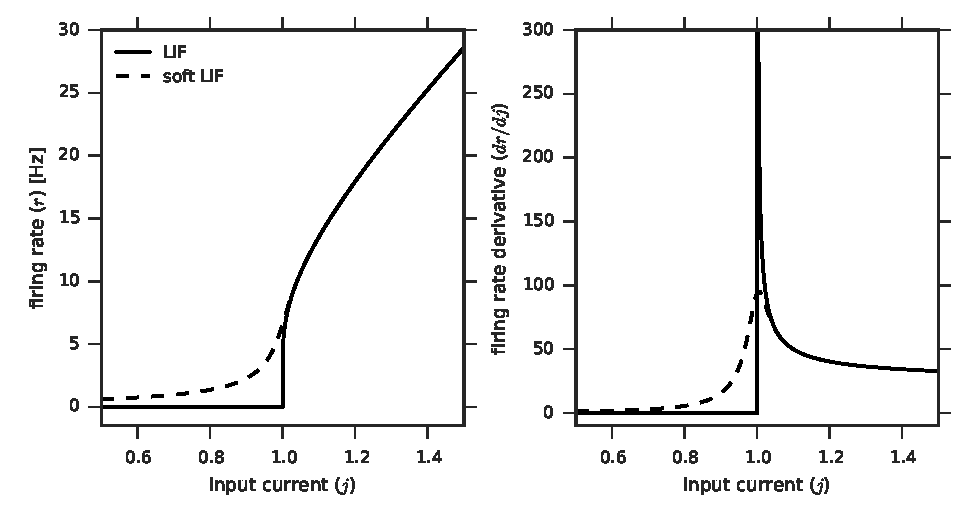
\includegraphics[width=6in]{softlif.pdf}
  \captionb{Comparison of LIF and soft-LIF response functions.}{
    The left panel shows the response functions themselves.
    The LIF function has a hard threshold at $j = V_{th} = 1$;
    the soft-LIF function ($\gamma = 0.01$) smooths this threshold.
    The right panel shows the derivatives of the response functions.
    The hard LIF function has a discontinuous and unbounded derivative
    at $j = 1$; the soft-LIF function has a continuous bounded derivative,
    making it amenable to use in backpropagation.
  }
  \figlabel{softlif}
\end{figure}

By replacing this hard maximum with a softer maximum,
such as $\rho_1(x) = \log(1 + e^x)$,
we can smooth over the hard firing threshold of the LIF neuron.
This smoothed equation is no longer discontinuous in its derivative;
the derivative is bounded.
Further, we can use the substitution
\begin{align}
  \rho_2(x) = \gamma \log\left[1 + e^{x / \gamma}\right]
  \eqnlabel{softrelusigma}
\end{align}
to allow us control over the amount of smoothing,
where $\rho_2(x) \to \max(x, 0)$ as $\gamma \to 0$.
\fig{softlif} compares of the LIF and soft-LIF rate response functions.

By reducing $\gamma$, we can make the soft-LIF rate response function
arbitrarily close to the LIF rate response function,
allowing the soft-LIF function to accurately model
the firing rates of the spiking LIF neurons used during testing.
Of course, having $\gamma$ be too small results in the same
ill-behaved derivative that the soft-LIF model is designed to avoid,
making the choice of $\gamma$ an empirical tradeoff.
In practice,
the precise choice of $\gamma$ does not appear to have
a large effect on network accuracy.
As long as the network does not learn to rely on the small activation
that the soft-LIF neuron has below the LIF neuron firing threshold,
then switching from soft-LIF to LIF neurons will not introduce significant error.
Since a classification network is trying to differentiate between different classes,
it tends to want individual neurons to be selective between classes,
responding strongly in the presence of some classes
and being silent in the presence of others.
This is does not mean that the input driving any particular neuron
is bimodally distributed;
in fact, the input currents across all neurons in a layer
appear unimodally distributed.
Rather, a neuron looking to be strongly and robustly representative of a class
will form strong connections with the strongly and robustly activated neurons
in the previous layer,
since these are the most reliable for classification.
Thus the network will not tend to rely on the weak activations of many neurons,
and the below-threshold activation of the soft-LIF model
should have minimal effect.

This is especially the case when training with noise (\scn{noise-models}).
Noise on the inputs to a neuron is more detrimental
when the neuron is active in an area of its rate-response curve with a large derivative,
since fluctuations in the input will have larger effects on the output.
For the LIF neuron, the rate-response derivative is highest at the firing threshold,
and lowest below the firing threshold (where it is zero)
and well above it (where it approaches zero).
Additionally, filtered spike trains show the most variability
when the firing rate is low (see \fig{lifvariance}).
Both of these factors penalize neuron activities around the firing threshold,
since these result in the most variable outputs.
The result is that neural activations near the firing threshold
should not be relied on by the network,
and switching from soft-LIF to LIF neurons should have little effect.

%% The fact that noise can cause sub-threshold neural firing
%% actually forms the biological motivation for the soft-LIF curve.
The soft-LIF curve has a biological motivation.
High-frequency variability (``noise'') in the membrane voltage of a neuron,
caused for example by random fluctuations in ion-channel opening and closing
\parencite{Manwani1999},
can cause a neuron to fire for a constant input that is slightly below
its firing threshold.
Thus, the response of a LIF neuron model with noise in the membrane voltage
looks qualitatively similar to the soft-LIF response function.
The response of such a noisy LIF neuron
can be modelled using the Siegert approximation
\parencite{Siegert1951,Kreutz-Delgado2015}.
This approximation requires numerically computing an integral
across a complex integrand.
The soft-LIF function provides a similar effect
while being much simpler to implement,
making it more amenable for training networks on GPUs, for example.


\subsection{Modelling spiking variability}
\scnlabel{noise-models}

A key difference between spiking and rate networks
is that spiking networks have much more variability
in the signals passed between neurons.
The output of a spiking neuron (\ie/ a series, or ``train'', of spikes)
is highly variable;
the signal is very large at some points in time (when a neuron spikes),
and zero at all other points in time (between spikes).
Luckily, synapses have an effect of lowpass-filtering these signals (see \scn{synapses}),
reducing the variability.
Still, the variability of the filtered signal is significant.
%% The amount of variability also depends on the firing rate of the neuron
The result is that whereas a rate network will produce a constant output
given a constant input,
a spiking network will have a variable output even for a constant input.
Understanding how the synaptic filter affects a spike train is
the key to understanding variability in spiking networks,
and the first step in reducing its adverse effects.

\begin{figure}
  \centering
  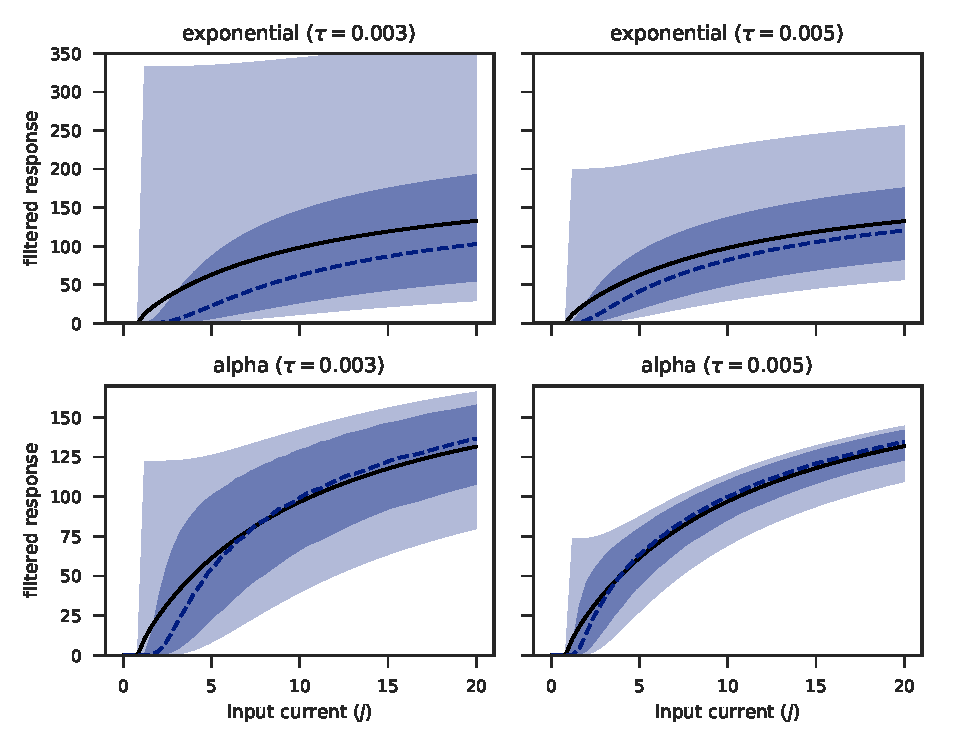
\includegraphics[width=\columnwidth]{lif_variance}
  \captionb{Effect of presynaptic input current on variance of postsynaptic current.}{
    The black line shows the average of the filtered postsynaptic signal
    (which is identical to the average firing rate given by \eqn{lifrate},
    since the filtering is linear).
    The dashed line shows its the median of this signal.
    The darker region indicates the range of its middle quartiles
    (25\sth/ percentile to 75\sth/ percentile).
    The lighter region indicates its full range (minimum to maximum).
  }
  \figlabel{lifvariance}
\end{figure}

\fig{lifvariance} shows the variability of filtered spike trains
across various levels of input current,
for different types of filtering.
Low levels of filtering (\eg/ the exponential filter with $\taus = 0.003$ s)
results in filtered spike trains that are highly variable.
Both increasing the synaptic time constant $\taus$
and increasing the order of the filter from first-order (exponential filter)
to second-order (alpha filter) reduce the amount of variability.
One significant difference between the two synapse models
is that the exponential synapse still has non-zero variance
even for large firing rates,
whereas with the alpha synapse the variance goes to zero
as the firing rate increases
(see \app{spike-model-limits} for a proof).
Due to the significantly lower variance of the alpha synapse,
it will be the main synapse model used in this thesis.

If we can mimic the effects of this spiking variability when training networks,
then ideally the network will become more robust to that variability,
and the resulting networks will run better in spiking neurons
than those trained without noise.
To do this, we need a model that can mimic the variability
in the neuron output given the neuron's firing period $p$.
The first model I experimented with was a simple Gaussian noise model:
\newcommand{\mgauss}{m_\text{G}}
\begin{align}
  \mgauss(p) = \begin{cases}
    \frac{1}{p} + N(0, \sigma) & \text{if } \frac{1}{p} > r_1 \\
    \frac{1}{p}                & \text{otherwise}
  \end{cases} \text{ .}
\end{align}
That is, the noisy output of the neuron is equal to the firing rate
(the inverse of the firing period)
plus additive Gaussian noise with zero mean and standard deviation $\sigma$.
I only add noise if the firing rate is greater than $r_1 = r(j=1)$,
the firing rate of the neuron model at the firing threshold $j = 1$.
The idea behind this is to not add noise when the neuron is silent,
since there is no variability in that case.
The soft-LIF model's firing rate never becomes exactly zero, however,
it only approaches zero as $j \to -\infty$.
I thus chose to add noise only when the input current $j > 1$,
that is, when the corresponding LIF neuron would be firing.
The $\sigma$ parameter can be fit to the empirically-measured
spiking neuron output variance, as characterized in \fig{lifvariance}.
This makes the model amenable to any synapse model.
The main drawbacks to the model are that it models the noise as Gaussian
(which it is not, particularly for low firing rates, see \fig{lifvariance}),
and that it treats the amount of variance as constant across all firing rates
(which again is not the case).

For certain synapse models---including the alpha synapse---%
we can more accurately model the variability of a filtered spike train.
Making the assumption that neurons in the network
are all spiking at constant rates,
we can model the variability in the network
by applying a synaptic filter to a train of spikes at regular intervals,
and looking at the resulting signal.
The result of filtering a spike train with an alpha synapse is given by:
\newcommand{\salpha}{s_\alpha}
\newcommand{\malpha}{m_\alpha}
\begin{align}
  \salpha(t) &= \frac{e^{-t/\taus}}{\taus^2} \left(
    \frac{t}{1 - e^{-p/\taus}} + \frac{p e^{-p/\taus}}{\left(1 - e^{-p/\taus}\right)^2} \right)
  \eqnlabel{alpha-model}
\end{align}
where $\taus$ is the synaptic time constant
and $p$ is the period between spikes.\footnote{
  A full derivation for this equation is given in \app{spike-derivations},
  \eqn{alpha-series}.}

% --- using this noise in real networks is too much variability at lower spike
%   rates. Real networks integrate info over time, less affected by noise.
We can use the alpha-filtered impulse train series
to generate noise in a rate-based network during training,
to help simulate the variability caused by spikes.
To do this, we assume that each input neuron is firing at a constant rate,
and that at any given point in time,
the time since the last spike of the neuron is uncorrelated with all other neurons
(\ie/ firing is completely desynchronized).
To sample from \eqn{alpha-model} for a neuron with firing period $p$,
I generate a random $t \sim U(0, p)$
(that is, $t$ is uniformly distributed between zero and $p$).
Thus, the alpha noise model describes the noisy output of a neuron
with firing period $p$ as $\malpha(p) = \salpha(U(0, p))$.

Despite the fact that \eqn{alpha-model} perfectly models
the filtered output of a regularly-spiking neuron,
it is actually a poor model for spike noise
because it over-estimates the variability in the network due to spikes.
This is because spiking neurons integrate information over time,
helping to smooth out the large fluctuations present in \eqn{alpha-model}.
To account for this, I combined the effects of the synaptic filter
with the filtering effects of the postsynaptic neural membrane.
Applying this combined filter to a spike train results in the following model:
\newcommand{\salphatau}{s_{\alpha\tau}}
\newcommand{\malphatau}{m_{\alpha\tau}}
\begin{align}
  \salphatau(t) &= \frac{\taurc}{d^2}\left(
    \frac{e^{-t/\taurc}}{1 - e^{-p/\taurc}} - \frac{e^{-t/\taus}}{1 - e^{-p/\taus}}\right)
  - \frac{e^{-t/\taus} \left(t (1 - e^{-p/\taus}) + p e^{-p/\taus}\right)}
         {d \taus \left(1 - e^{-p/\taus}\right)^2} \text{ ,}
  \eqnlabel{alpharc-model}
\end{align}
where $d = \taurc - \taus$.
The corresponding noise model is given by $\malphatau(p) = \salphatau(U(0, p))$.

\begin{figure}
  \centering
  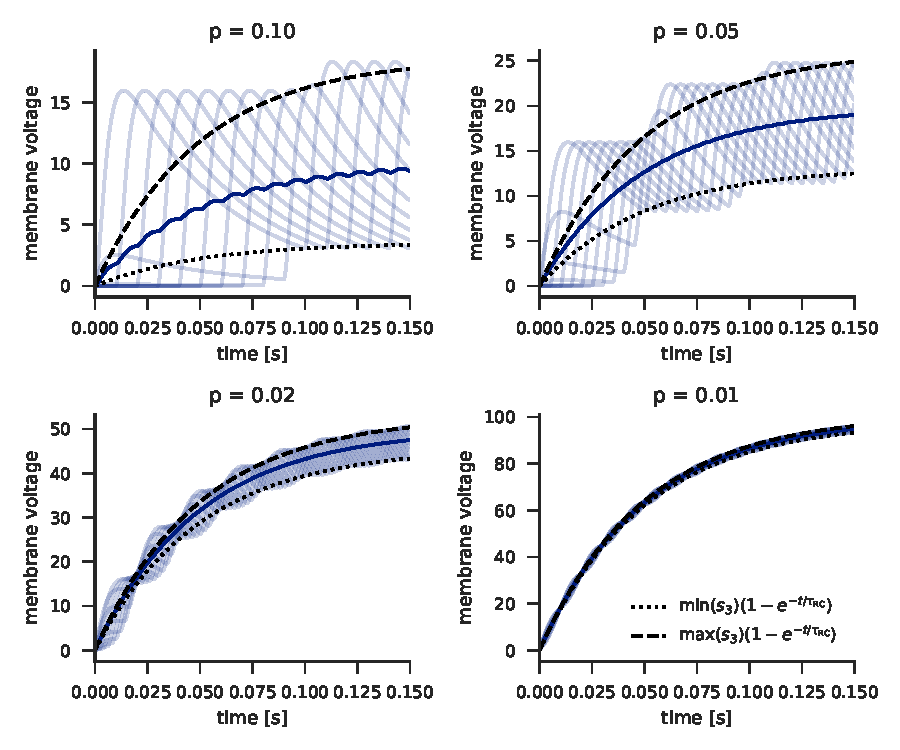
\includegraphics[width=\columnwidth]{alpharc_distribution}
  \captionb{Evaluation of the $\malphatau(t)$ noise model.}{
    To evaluate the $\malphatau(t)$ noise model (\eqn{alpharc-model}),
    I compared voltage traces of a neuron receiving input from an
    alpha-filtered spike train (solid blue traces),
    with an exponential increase to the minimum and maximum of $\salphatau(t)$
    (dotted and dashed traces).
    The light solid traces show individual neuron membrane voltages
    with different input spike train phases (offsets).
    The dark solid trace shows the average of the individual neuron traces.
    Each plot shows a different period $p$ for the input spike train.
    Since the neuron input is not modulated by connection weights,
    the membrane voltage is in arbitrary units.
    $\taurc = 0.05, \taus = 0.003$
  }
  \figlabel{alpharc-minmax}
\end{figure}

To evaluate how well $\salphatau(t)$ actually represents
the variability caused by spikes,
I examined how the range of this series compares to
the actual membrane voltages of an LIF neuron with an
alpha-filtered spike train input at different periods (\fig{alpharc-minmax}).
When we sample from $\salphatau(t)$ to generate a noisy output of a neuron
with spiking period $p$,
we get a value that represents the steady-state of the neuron membrane voltage;
that is, the membrane voltage will exponentially approach this value.
The neuron will spike when its membrane voltage crosses the firing threshold.
Because the connection weights can scale the input arbitrarily,
and scaling all inputs is equivalent to scaling the firing threshold,
we can view the firing threshold as being at any point of the y-axis
in \fig{alpharc-minmax}.
The point in time at which the voltage crosses the firing threshold
determines the firing rate.
The lighter solid lines in \fig{alpharc-minmax} show the membrane voltage
of an LIF neuron subject to an alpha-filtered spike train with period $p$,
given that the neuron has just fired a spike and the voltage is reset to zero.
Each line shows a different phase (\ie/ different temporal offset)
for the filtered input spike train.
The dashed lines show an exponential approach
to the minimum and maximum of $\salphatau(t)$.
These indicate the range of variability that we can get
by using the $\salphatau(t)$ distribution for noise generation in the model.
If we draw a horizontal line through any point in the graph
(corresponding to setting the neuron firing threshold at this value),
the places where the solid lines intersect will represent the range
of possible inter-spike intervals (ISIs) for an actual neuron with spiking input,
and the space between the dashed lines will represent the range
of possible inter-spike intervals using the $\salphatau(t)$ noise model.
If $\salphatau(t)$ represents well the variability caused by spikes,
then these two ranges should correspond well for any horizontal line we draw.
This would mean that wherever the firing threshold of the neuron is
(\ie/ whatever the magnitude of the inputs),
the actual variability caused by spikes will be well represented by the model.

As we see in \fig{alpharc-minmax},
the fit of the noise model depends on both the period of the input spike train
and the amount of time we allow for the membrane voltage to settle.
For all input spike periods $p$,
if we allow the membrane voltage sufficient settling time ($t > 3\taurc$),
then the $\salphatau(t)$ noise model represents the spiking variability well.
This corresponds to the situation when the firing rate of the
output neuron is low.
For higher input spike rates (smaller $p$),
the noise model also does a reasonably good job representing
the spiking variability for $t < 3\taurc$,
as shown in the bottom two panels.
In this situation, the output spike rate can be higher
while still having the variability be well modelled.
As the input spike rates get lower (larger $p$),
the noise model gets progressively worse at capturing
the full range of variability caused by spikes
before the voltage has had time to settle,
as shown by the light solid traces not falling
within the dotted and dashed lines at earlier times.
The worst case scenario is when input spike rates are low,
but the output spike rate is high (\ie/ an ISI of less than $\taurc$).
In this case, the model severely underestimates
the amount of variability caused by spikes.
In practice, this seems to be an uncommon situation,
since the firing rate of neurons
typically decreases from one layer to the next (see \tab{spike-rates}).

\begin{figure}
  \centering
  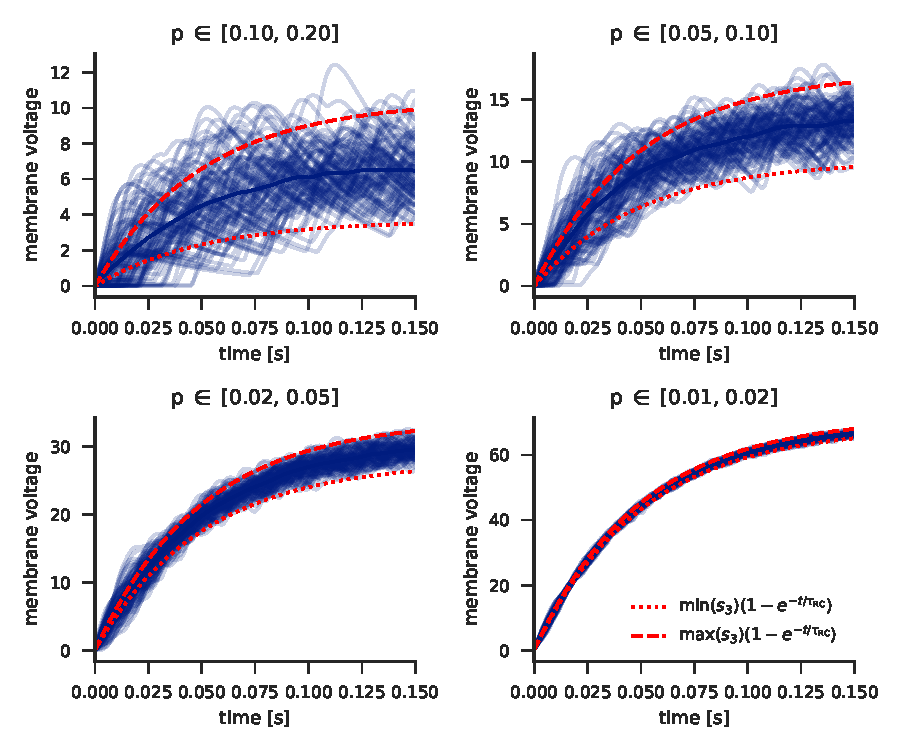
\includegraphics[width=\columnwidth]{alpharc_multiperiod}
  \captionb{Evaluation of the $\malphatau$ noise model with multiple inputs.}{
    Each neuron gets five alpha-filtered spike train inputs,
    with periods $p$ linearly spread across the given ranges (separate panels).
    Each light trace shows one trial (100 trials total),
    where the phases (temporal offsets) of each input are determined randomly.
    The dotted and dashed lines show the minimum and maximum across all trials
    of the noise model,
    where the value of the noise model for one trial is the mean across the
    nine neurons of $\salphatau(t)$ evaluated at the period and offset time for that neuron.
    Since the neuron input is not modulated by connection weights,
    the membrane voltage is in arbitrary units.
    $\taurc = 0.05, \taus = 0.003$
  }
  \figlabel{alpharc-multineuron}
\end{figure}

So far, this analysis has considered the case
when we have a single input neuron,
but in actual networks, each neuron gets input from multiple neurons.
\fig{alpharc-multineuron} looks at this case.
It makes the assumption that we have nine input neurons,
all with the same input weighting and randomly chosen phases,
and with firing periods spread uniformly between two values (distinct for each panel).
This analysis shows similar results as before:
when the membrane voltage is allowed to relax towards its steady state,
the noise model performs well.
For shorter filtering times (\ie/ fast output firing rates)
and for longer input periods,
the model underestimates the variability caused by spikes.
However, the magnitude of these errors is generally smaller,
due to the fact that some of the variability caused by the different inputs
cancels out, assuming the neurons are not synchronized.


\subsection{Training methods}
\scnlabel{spike-training}

To train the network,
I used backpropagation to determine the parameter gradients (\scn{backprop}),
and stochastic gradient descent as an optimization strategy (\scn{sgd}).
This is the same method used by \textcite{Krizhevsky2012},
and is common for training deep neural networks.

For the most part,
the architectural modifications described in \scn{spike-architecture}
had little effect on the training procedure.
One exception is that the parameters used for the LIF neurons---%
namely the bias, gain, amplitude, $\taurc$, $\tref$, and $\gamma$---%
had a large effect on the success of the training.
The most important factor when choosing all of these parameters
is that for the initial weights and biases in the network,
the derivatives of the nonlinearities for inputs from the dataset
should be around one.
This helps to discourage both the vanishing gradient problem
(where the gradient in the lower layers becomes too small),
and the exploding gradient problem
(where the gradient becomes too large).
For ReLU nonlinearities, this is easy,
since the derivative of a ReLU is one whenever it is active.
This is one characteristic that makes training networks with ReLUs much easier,
but it is not the case with the LIF (or soft-LIF) nonlinearity.
By default, the firing threshold of a LIF neuron corresponds to $J = 1$,
so the first change that I made is to give it a bias of one
such that the firing threshold is at zero.
Second, I chose the membrane time constant ($\taurc$) of the neurons.
Smaller values ($\taurc = 0.02$) caused problems with training,
so I chose $\taurc = 0.05$,
which makes a smoother transition between the silent and spiking regimes
of the neuron, and thus a less extreme gradient.
It is possible that shorter $\taurc$ can be used
if other parameters---such as the magnitudes of the initial weights---%
are more judiciously chosen.
I chose $\tref = 0.001$ to be small,
to reduce the effects of saturation on neuron behaviour.
I found that $\gamma$---the amount of smoothing for the ``soft'' LIF---%
could actually be quite small and still train successfully;
I chose $\gamma = 0.02$.
Smaller $\gamma$ is desirable because it makes the soft-LIF curve
closer to the LIF curve,
thus creating less error when switching to spiking neurons.
Finally, I chose the neuron gain and amplitude
(that is, multiplicative scaling on the input and output, respectively)
such that the soft-LIF curve fit the ReLU curve as closely as possible
for inputs in the range $[-1, 10]$.
This ensures that both the magnitude of the soft-LIF output
is in a reasonable range,
and that the soft-LIF derivative has a maximum around one.

The ImageNet (ILSVRC-2012) dataset required one additional modification:
initial pretraining over a few ($\sim$30) batches using a small learning rate,
to bring the initial parameters into a more reasonable range.
Otherwise, beginning with a normal learning rate
would lead to instability in the training.


\subsection{Evaluation methods}
\scnlabel{spike-evaluation}

When evaluating the network,
all off the rate-based (soft-LIF) neurons are replaced with spiking LIF neurons,
and the network is run online.
The spiking classification procedure is the same as in the previous chapter
(see \scn{nef-spiking-methods}).
As with those networks,
the amount of time required to get a reasonable classification result
is an empirical question,
depending on the synaptic time constant $\taus$
and how small we wish to make the margin of error between the spiking network
and its ANN counterpart;
I examine this in \scn{spike-efficiency}.

% no multiview testing
One key difference with \textcite{Krizhevsky2012}
is that they used multiview testing:
many (9) different image patches (chosen in a $3 \times 3$ grid covering the image)
are all passed through the classifier,
and the final classification is determined by averaging the softmax outputs
across all views,
and taking the class with the highest average.
Presenting multiple views requires multiple passes through the network,
which is not realistic for a spiking network.
Each view could be presented sequentially,
but this would take significantly more processing time.
I also experimented with jittering the input image over time
to simulate the effect of multiple views in a shorter time scale;
this did not lead to better classification results.

These models were run using the Nengo simulator \parencite{Bekolay2014}.
In particular, the Nengo OCL backend\footnote{
  \url{https://github.com/nengo/nengo_ocl}}
was used to run the networks efficiently on a GPU.
I made significant additions to the backend
specifically for running convolutional networks efficiently.

%% Another key difference with some other works is that here,
%% each stimulus is presented in series without resetting the network
%% in between presentations \parencite[\cf/][]{Cao2014,Diehl2015}.
%% Each stimulus is also only presented once,
%% which differs from \textcite{Diehl2015} who present each stimulus
%% five times and average over


\section{Results}
\scnlabel{spike-results}

This section provides results from training and running
the spiking network on the datasets described in \scn{datasets}.
The experiments comparing the effects of noise on network training and testing
are performed on the CIFAR-10 dataset,
since it is sufficiently small to allow training many networks (for robust results).


\subsection{System overview}

\begin{figure}
  \centering
  %% 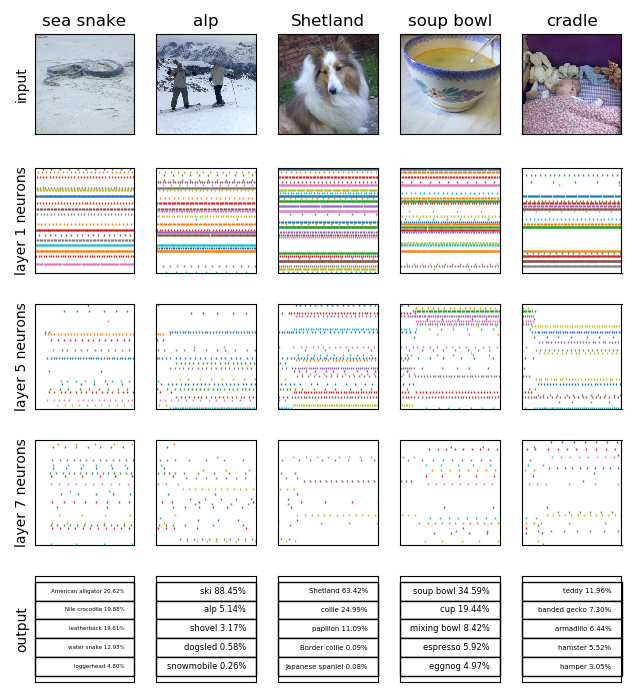
\includegraphics[width=5.8in]{imagenet_demo.png}
  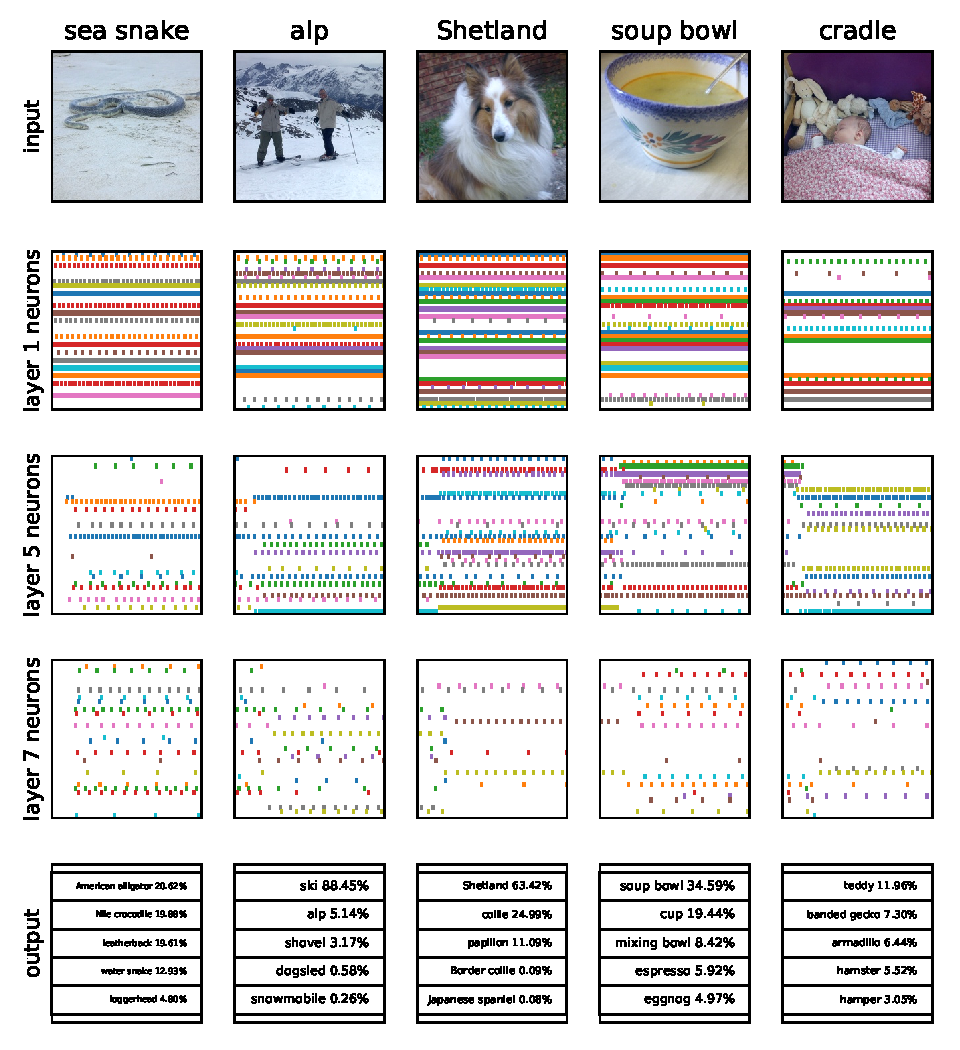
\includegraphics[height=6.4in]{imagenet_demo.pdf}
  \captionb{The spiking system running on several ImageNet images.}{
    Images are presented to the network (top row),
    which processes them using seven layers of spiking neurons (middle three rows).
    The activities in the final spiking layer are decoded to
    probabilities of membership in each of the 1000 possible classes
    (the five most probable classes are shown).
    A video demonstration is available at \url{https://youtu.be/VWUhCzUDZ70}.
  }
  \figlabel{imagenet-demo}
\end{figure}

\fig{imagenet-demo} provides an overview of the system
running on ImageNet test images.
As images are presented sequentially to the network (top row),
they result in spiking activity through the various layers in the network
(middle rows).
The output of the system is weightings on all of the object categories,
which can be used to assign probabilities and predict the class of the image
(bottom row).
The synapses between subsequent layers in the network,
as well as the neural dynamics themselves,
both contribute to delays between successive layers.
Most of the first layer neurons respond almost instantaneously
to a change in the input stimulus,
but later layers take longer to transition to the new activity regime.
The model is often able to correctly predict the object class,
either as its first guess (see ``Shetland'' and ``soup bowl'')
or in its top five guesses (see ``alp'').
Even when the model is not correct, it is often in the right ballpark,
guessing similar objects (see ``sea snake'').
Sometimes, the model is wildly incorrect,
as in the case of ``cradle'' when it guesses ``banded gecko'',
``armadillo'' and ``hamster''
(though the first guess, ``teddy'', is accurate).
These images also illustrate the difficulty of the ImageNet dataset,
which is why researchers typically focus on having the correct category
in the top five guesses of the system,
rather than requiring the system to guess the correct class outright.


\subsection{Architecture modifications and noise}

This section examines the effects of different modifications
to the architecture on the CIFAR-10 dataset.
The starting point is a network trained as per \textcite{Krizhevsky2012}.
The measured test-set error (14.03\%) is considerably higher than
the number reported by \textcite{Krizhevsky2012} ($\sim$11\%),
mainly because the version presented here does not use multiview testing,
whereas the original work does (see \scn{spike-evaluation}).

\begin{table}
  \begin{minipage}{\columnwidth}
  \centering
  \begin{tabular}{llr}
    \# & Modification & CIFAR-10 error \\\hline\hline
    0 & Original ANN \footcite[Based on][]{Krizhevsky2012} & 14.03\% \\
    1 & Network 0 minus normalization & 14.38\% \\
    2 & Network 1 with average-pooling & 16.70\% \\\hline
    3 & Network 2 with soft-LIF & 15.89\% \\  % cifar10-lif-1589
    4 & Network 3 with training noise ($\sigma = 10$) & 16.01\% \\  % cifar10-lif-1628
    5 & Network 3 with training noise ($\sigma = 20$) & 16.92\% \\\hline  % ?
    6 & Network 3 ($\sigma = 0$) in spiking neurons & 17.01\% \\
    7 & Network 4 ($\sigma = 10$) in spiking neurons & \textbf{16.46\%} \\
    8 & Network 5 ($\sigma = 20$) in spiking neurons & 17.04\% \\
  \end{tabular}
  \end{minipage}
  %% \vspace{0.2em}
  \captionb{Effects of successive architectural modifications to CIFAR-10 error.}{
    We first show the original ANN based on \textcite{Krizhevsky2012},
    and then the effects of each subsequent modification.
    Rows 6-8 show the results of running ANNs 3-5 in spiking neurons, respectively.
    Row 7 is the best spiking network, using a moderate amount of training noise.
    While these values provide a rough qualitative characterization
    of the effects of the architectural modifications,
    each error measurement only represents one network trained
    with a particular set of hyperparameters.
    A more robust analysis of the effects of training with noise
    is presented in the next section.
  }
  \tablabel{archmods}
\end{table}

The full list of modifications and the associated error measurements
are shown in \tab{archmods}.
The first modification (Network 1) removes the cross-map response normalization layers,
which only affects the test-set accuracy slightly ($\sim 0.3\%$).
The second modification (Network 2) replaces max-pooling with average-pooling,
which is more detrimental to the accuracy ($\sim 2.3\%$).

Network 3 introduces soft-LIF neurons.
This network is now a rate-based version of the final spiking network,
and thus serves as a baseline for the performance of later networks.
Surprisingly, the error rate of Network 3 is lower than that of Network 2,
that is, introducing soft-LIF neurons increases the accuracy of the network (by $\sim 0.8\%$).
However, this result is not necessarily significant.
Network accuracy depends heavily on the hyperparameters used \parencite{Bergstra2012},
and even slightly on the random initial values chosen for the learned parameters.
Thus, without extensive hyperparameter optimization,
we cannot draw the conclusion that the soft-LIF neuron is better than ReLUs,
even for this particular network.

Network 6 shows Network 3 run in spiking neurons.
I also trained two networks with moderate (Network 4) and high (Network 5)
amounts of Gaussian noise on the neuron firing rates,
and ran these networks in spiking neurons (Networks 7 and 8).
As shown by Networks 4 and 5,
training with even moderate noise reduces the accuracy of the network
(by $\sim 0.1\%$, not necessarily significant),
with more noise being more detrimental to performance ($\sim 1.0\%$).
However, when running in spiking neurons,
the network trained with a moderate amount of noise performs the best
(by $\sim 0.5\%$).
This demonstrates that the right amount of training noise
is able to make the network somewhat robust to the variability that
comes with running the network in spiking neurons.
This result is explored more robustly in the following section.


\subsection{Performance of noise models}
\scnlabel{spike-noise-results}

The previous section demonstrated that adding noise (with the Gaussian model)
can help to reduce the error in spiking networks.
To more robustly assess the benefits of training with noise,
I trained multiple (5) models on CIFAR-10 using the Gaussian noise model
with two different levels of noise,
as well as the models developed in \scn{noise-models},
specifically $\salpha$ (\eqn{alpha-model}) and $\salphatau$ (\eqn{alpharc-model}).
The results are shown in \tab{cifar10-noisemodels}.

\begin{table}
  \centering
  \begin{tabular}{lrrrrr}
    Noise model &
    \multicolumn{1}{c}{ANN} &
    \multicolumn{1}{c}{Spiking 1} &
    \multicolumn{1}{c}{Spiking 2} &
    \multicolumn{1}{c}{Spiking 3} &
    \multicolumn{1}{c}{Spiking 4} \\\hline
None &
15.57 (0.19) & 17.86 (0.30) & 16.99 (0.35) & 16.38 (0.19) & 16.31 (0.26) \\
$\mgauss$ ($\sigma = 10$) &
16.03 (0.12) & 17.15 (0.09) & 16.68 (0.22) & 16.38 (0.08) & 16.40 (0.13) \\
$\mgauss$ ($\sigma = 20$) &
16.96 (0.14) & 17.44 (0.24) & 17.29 (0.12) & 17.37 (0.12) & 17.43 (0.15) \\
$\malpha$ ($\taus = 3$ ms) &
18.49 (0.22) & 18.66 (0.24) & 18.48 (0.18) & 18.72 (0.28) & 18.68 (0.26) \\
$\malpha$ ($\taus = 5$ ms) &
16.96 (0.19) & 17.42 (0.32) & 17.22 (0.12) & 17.13 (0.20) & 17.20 (0.21) \\
$\malphatau$ ($\taus = 3$ ms) &
15.65 (0.30) & 17.31 (0.26) & 16.55 (0.27) & 16.18 (0.23) & 16.18 (0.25) \\
$\malphatau$ ($\taus = 5$ ms) &
15.66 (0.17) & 17.58 (0.34) & 16.90 (0.26) & 16.38 (0.20) & 16.37 (0.17) \\
  \end{tabular}
  \vspace{0.2em}
  \captionb{CIFAR-10 results from spiking networks trained with different noise models.}{
    Results are the average over five independent networks;
    the standard deviation is shown in parentheses.
    The columns show results for the non-spiking ANN,
    and spiking results using alpha synapses with:
    1) $\taus = 0$ ms, $t_c = 10 ms$, $t_p = 60 ms$;
    2) $\taus = 0$ ms, $t_c = 10 ms$, $t_p = 80 ms$;
    3) $\taus = 3$ ms, $t_c = 60 ms$, $t_p = 150 ms$;
    4) $\taus = 5$ ms, $t_c = 100 ms$, $t_p = 200 ms$.
    Noise, in the right amounts, is able to improve spiking performance,
    particularly in cases where the synapse time constant $\taus$
    used at runtime is small or zero,
    and the amount of time used for classification ($t_p$ minus $t_c$) is short.
    Note that for noise models that use a synapse time constant $\taus$,
    the value of $\taus$ used during training
    (presented with the noise model in the left-most column)
    does not necessarily match the value of $\taus$ used at runtime
    (which varies between the four spiking configurations).
  }
  \tablabel{cifar10-noisemodels}
\end{table}

The most salient result is that training with noise
is most beneficial for spiking networks
when the synapse time constant $\taus$ is small or zero
and the amount of time used for classification is short.
When training the ANN, the noise from the $\malphatau$ model has little effect
on the ANN performance,
whereas noise from the other models (which is generally larger in magnitude)
has on average an adverse effect on ANN performance.
In the first two spiking conditions, when no synapse is used ($\taus = 0$ ms),
the benefits of training with noise are most apparent:
networks trained with the $\malphatau$ model with $\taus = 3$ ms
perform significantly better than networks trained without noise.
The Gaussian noise model with $\sigma = 10$ also performs well in these cases.
When the synapse time constant is longer (3 ms or 5 ms),
the networks trained with either the $\malphatau$ model with $\taus = 3$
or the Gaussian noise model with $\sigma = 10$
perform about as well on average as the networks trained without noise.

The $\malphatau$ model with $\taus = 5$ ms performs closer to the no noise model case;
the higher level of filtering associated with this model
results in only a small amount of noise being added,
and it appears the reduced noise is not enough to significantly affect training.
The $\malpha$ noise model, on the other hand, generally introduces too much noise,
performing considerably worse then the other models across almost all cases;
the same is true of the Gaussian noise model with high noise ($\sigma = 20$).
The exception is when there is no synapse and short classification time (case 1),
when some of the higher-noise models are competitive.


\subsection{Accuracy on various datasets}
\scnlabel{spike-accuracy}

To better quantify the performance of my method of constructing spiking deep networks,
I measured its performance on five datasets,
and compared the results with other state-of-the-art spiking networks.
I used the MNIST, SVHN, CIFAR-10, CIFAR-100, and ImageNet datasets,
described in detail in \scn{datasets}.

A summary of the best test-set error scores are shown in \tab{spike-results}.
On all datasets, the network of spiking LIF neurons (LIF SNN)
is able to achieve results close to that of the non-spiking ReLU network (ReLU ANN).
This both shows that loss is minimal
when going from ReLUs to rate LIF neurons,\footnote{
  The CIFAR-100 dataset shows a considerable increase in performance
  when using soft-LIF neurons versus ReLUs in the ANN.
  However this may not be significant;
  it could simply be due to the training hyperparameters chosen,
  since these were not optimized in any way.}
and that loss is minimal when going from rate LIF neurons to spiking LIF neurons.\footnote{
  The ILSVRC-2012 dataset actually shows a marginal increase in accuracy
  when switching to spiking neurons.
  This is likely not statistically significant,
  and could be because the spiking LIF neurons have harder firing thresholds
  than their soft-LIF rate counterparts.}

\begin{table}
  \centering
  \begin{minipage}{\columnwidth}
    %% \begin{center}
    %% \begin{tabular}{|l|r|r|r|}\hline
    %%   Dataset & ReLU ANN & LIF ANN & \textbf{LIF SNN} \\\hline\hline
    %%   MNIST & 0.79\% & 0.84\% & 0.88\% \\\hline
    %%   SVHN & 5.65\% & 5.79\% & 6.08\% \\\hline
    %%   CIFAR-10 & 16.48\% & 16.28\% & 16.46\% \\\hline
    %%   CIFAR-100 & 50.05\% & 44.35\% & 44.87\% \\\hline
    %%   ILSVRC-2012 & 45.4\% (20.9\%)$^a$ & 48.3\% (24.1\%)$^a$ & 48.2\% (23.8\%)$^a$\\\hline
    %% \end{tabular}
    %% \end{center}
    %% \vspace{-0.2em}
    %% \hspace{5em}$^a$ Results from the first 3072-image test batch.
    \begin{center}
    \begin{tabular}{lrrrrr}
      Network  & MNIST & SVHN & CIFAR-10 & CIFAR-100 & ILSVRC-2012\footnote{
        Results from the first 3072-image test batch.}\\\hline
      ReLU ANN & 0.79 & 5.65 & 16.48 & 50.05 & 45.4 (20.9) \\
      LIF ANN  & 0.84 & 5.79 & 16.28 & 44.35 & 48.3 (24.1) \\
      LIF SNN  & 0.88 & 6.08 & 16.46 & 44.87 & 48.2 (23.8) \\
    \end{tabular}
    \end{center}
  \end{minipage}
  \captionb{Test-set error rates (percent) for spiking LIF networks (LIF SNN).}{
    Compared with ReLU ANN and LIF ANN (both using the same network structure,
    but with ReLU and LIF rate neurons respectively).
    The spiking versions of each network perform
    almost as well as the rate-based versions.
    The ILSVRC-2012 (ImageNet) results show the error for the top result,
    with the top-5 result in brackets.
  }
  \tablabel{spike-results}
\end{table}

\begin{table}
  \centering
  \begin{minipage}{\columnwidth}
    \begin{center}
    \newcommand{\cmpesser}{\label{cmpesser}\textcite{Esser2016}}
    \newcommand{\cmpbatch}{\label{cmpbatch}Results from the first 3072-image test batch.}
    \begin{tabular}{lrrrrr}
      Dataset & \textbf{My model} &
        TN 1-chip\footnote{\cmpesser} &
        TN 8-chip\footnoteref{cmpesser} &
        Zambrano\footcite{Zambrano2017} &
        Best Other \\\hline
      MNIST       & 0.88 (27k) &           &           & 0.44 (100k) & 0.88 (22k) \footcite{Diehl2015} \\
      SVHN        & 6.08 (27k) & 3.34 (1M) & 2.54 (8M) &      & \\
      CIFAR-10    & 16.46 (50k) & 16.59 (1M) & 10.68 (8M) & 10.14 (270k) & 22.57 (28k) \footcite{Cao2014} \\
      CIFAR-100   & 44.87 (50k) & 44.36 (1M) & 34.52 (8M) & 35.79 (295k) & \\
      ILSVRC-2012 & 48.2\footnote{\cmpbatch} (493k) & & & 37.03 (24M) & \\
    \end{tabular}
    \end{center}
  \end{minipage}
  \captionb{Percentage error rates of my model compared with state-of-the-art models.}{
    I compare with recent results on the TrueNorth (TN) neuromorphic chip \parencite{Esser2016},
    as well as other best results in the literature.
    Approximate numbers of neurons are shown in parentheses.
    The TrueNorth networks use significantly more neurons than my networks
    (about 20$\times$ more for the 1-chip network
    and 160$\times$ more for the 8-chip network).
    The ILSVRC-2012 (ImageNet) numbers indicate the error for the top result
    (the top-5 result for this work can be found in \tab{spike-results},
    and was not reported for Zambrano).
    It is important to note that my error on ILSVRC-2012 is only computed
    using the first 3072-image test batch (to reduce computation time),
    and thus only provides an estimate of the true error
    and is not directly comparable to the other result on this dataset.
  }
  \tablabel{spike-comparison}
\end{table}


\tab{spike-comparison} compares my results
with several other state-of-the-art results for deep spiking networks.
A recent paper using the TrueNorth neuromorphic chip \parencite{Esser2016}
set many new records for spiking networks
on the SVHN, CIFAR-10, and CIFAR-100 datasets.
However, these networks use large numbers of neurons,
either one million for the one-chip networks
or eight million for the eight-chip networks.
By comparison, my networks---%
which use orders of magnitude fewer neurons (27-50 thousand)---%
outperform the one-million-neuron TrueNorth networks
on two of the three tasks.
Furthermore, I demonstrate that my methods can perform reasonably well
on the very large ImageNet (ILSVRC-2012) dataset using half a million neurons.
The methods used by \textcite{Esser2016}
would have difficulty scaling a problem of this size due to the sheer
number of neurons required.


\begin{table}
  \centering
  \begin{minipage}{\columnwidth}
    \begin{center}
      \newcommand{\ratbatch}{\label{ratbatch}Results from the first 3072-image test batch.}
      \newcommand{\hunsa}{\textbf{My model}}
      \newcommand{\hunsb}{\hunsa}
      \newcommand{\zamba}{Zambrano\footnote{\label{zamba}\textcite{Zambrano2017}}}
      \newcommand{\zambb}{Zambrano\footnoteref{zamba}}
      \begin{tabular}{llrrrrr}
        Dataset & Method & Error & Neurons & Rate & Time & Spikes/image \\
        \hline\multirow{3}{*}{MNIST}
            & \hunsa & 0.88 & 27.1 k & 9.7 & 200 & 52 k \\
            & \zamba & 0.44 & 100.7 k & 67 & 291 & 1963 k \\
            & \zambb & 0.88 & 100.7 k & 10 & 209 & 210 k \\
        \hline\multirow{3}{*}{CIFAR-10}
            & \hunsb & 16.5 & 49.5 k & 148 & 200 & 1.5 M \\
            & \zambb & 10.1 & 270.8 k & 68 & 372 & 6.9 M \\
            & \zambb & 11.5 & 270.8 k & 22 & 304 & 1.8 M \\
        \hline\multirow{3}{*}{Imagenet}
            & \hunsb & 48.2\footnote{\ratbatch} & 493.2 k & 93 & 200 & 9.2 M \\
            & \zambb & 37.0 & 24085 k & 66 & 347 & 551.6 M \\
            & \zambb & 46.2 & 24085 k & 12 & 338 & 97.7 M
      \end{tabular}
    \end{center}
  \end{minipage}
  \captionb{Comparison of spikes required to classify an image.}{
    Comparing my method with another state-of-the-art method
    (the only method from \tab{spike-comparison} to report overall network firing rates).
    Despite higher firing rates,
    my model uses fewer spikes to classify each image,
    due to the significantly fewer neurons used.
  }
  \tablabel{spike-sota-rates}
\end{table}

It is only quite recently that other another spiking network
has been able to compete on ILSVRC-2012,
namely that of \textcite{Zambrano2017}.
Their networks also use lower firing rates than other state-of-the-art networks
(including the ones presented in this thesis).
However, their networks also use significantly more neurons
than those presented in this thesis.
The result is that the number of spikes required to classify each image
is actually higher than all the networks presented in this thesis
(see \tab{spike-sota-rates}).


\subsection{Efficiency}
\scnlabel{spike-efficiency}

\newcommand{\Esnn}{E_\text{SNN}}
\newcommand{\Esynop}{E_\text{synop}}
\newcommand{\Eupdate}{E_\text{update}}

Running on standard hardware,
spiking networks are considerably less efficient
than their ANN counterparts.
This is because ANNs are static,
requiring only one forward-pass through the network to compute the output,
whereas SNNs are dynamic,
requiring the input to be presented for a number of time steps
and thus a number of forward passes.
On hardware that can take full advantage of the sparsity that spikes provide---%
such as most neuromorphic hardware---%
SNNs can be more efficient than the equivalent ANNs, as we show here.

First, we need to compute the computational efficiency of the original network,
specifically the number of floating-point operations (FLOPs) required to pass
one image through the network.
The two main computations in a spiking neural network
are those associated with the neurons,
and those associated with the connections:
\begin{align}
  \text{FLOPs} &= \frac{\text{FLOPs}}{\text{neuron}} \times \text{neurons} +
                  \frac{\text{FLOPs}}{\text{connection}} \times \text{connections} \text{ .}
\end{align}
Since a rectified linear unit is a simple max function,
it requires only one FLOP to compute ($\text{FLOPs/neuron} = 1$).
Each connection requires two FLOPs, a multiply and an add ($\text{FLOPs/connection} = 2$).
We can determine the number of connections by ``unrolling'' each convolution,
so that the layer is in the same form as a locally connected layer.
(See \tab{network-sizes} for the number of FLOPs
needed to process a single image on conventional hardware
for each different network architecture.)

\begin{table}
  \centering
  \begin{tabular}{r|rrr|rrr|rrr}
    &
    \multicolumn{3}{c|}{MNIST} &
    \multicolumn{3}{c|}{CIFAR-10} &
    \multicolumn{3}{c}{ILSVRC-2012} \\
    Layer
      &  $N$  & $S$  &  $R$ &  $N$  & $S$  & $R$ & $N$  & $S$  & $R$  \\\hline
    0 &       & 314k &      &       & 2.8M &     &      &  70M &      \\
    1 & 12.5k & 5.0M &  4.6 &   37k &  15M & 173 & 194k & 224M & 178  \\
    2 & 12.5k & 6.3M & 15.6 &  9.2k & 1.3M &  99 & 140k & 112M & 48.8 \\
    3 &    2k &  20k &  4.2 &  2.3k & 664k & 9.7 &  65k & 150M & 26.6 \\
    4 &       &      &      &  1.2k &  12k & 7.2 &  43k & 100M & 30.6 \\
    5 &       &      &      &       &      &     &  43k &  38M & 35.6 \\
    6 &       &      &      &       &      &     & 4.1k &  17M & 19.1 \\
    7 &       &      &      &       &      &     & 4.1k & 4.1M & 10.7 \\
  \end{tabular}
  \captionb{Spike rates by layer for my networks.}{
    The number of neurons $N$, synapses out of the layer $S$, and average spike rate $R$ in Hz
    for each layer of each network (k = thousands, M = millions).
    Layer 0 indicates the input layer, which has no neurons,
    so only the synapses out are shown (connecting to the first hidden layer).
    The output layers, which also have no neurons, are not shown.
  }
  \tablabel{spike-rates}
\end{table}

To compute the SNN efficiency on a prospective neuromorphic chip,
we begin by identifying the energy cost
of a synaptic event ($\Esynop$) and neuron update ($\Eupdate$),
relative to standard hardware.
In consultation with neuromorphic experts,
and examining current reports of neuromorphic chips \parencite[\eg/][]{Merolla2014}),
we assume that
each neuron update takes as much energy as 0.25 FLOPs ($\Eupdate = 0.25$),
and each synaptic event takes as much energy as 0.08 FLOPs ($\Esynop = 0.08$).
(These numbers could potentially be much lower for analog chips, \textcite[\eg/][]{Benjamin2014}.)
Then, the total energy used by an SNN to classify one image is
(in units of the energy required by one FLOP on standard hardware):
\begin{align}
  \Esnn = \left(\Esynop \frac{\text{synops}}{\text{s}} +
            \Eupdate \frac{\text{updates}}{\text{s}}\right) \times
            \frac{\text{s}}{\text{image}} \text{ .}
  \eqnlabel{esnn}
\end{align}
These numbers are computed from the per-layer parameters
shown in \tab{spike-rates}:
\begin{align}
  \frac{\text{synops}}{\text{s}} &= \sum_i^L S_i R_i \nonumber\\
  \frac{\text{updates}}{\text{s}} &= \frac{\text{timesteps}}{\text{s}} \times \sum_i^L N_i \nonumber
  \text{ ,}
\end{align}
where $L$ is the number of layers.\footnote{
  The networks in this thesis update every millisecond,
  resulting in 1000 timesteps/s.}
The CIFAR-10 network has rates of
2.69 billion synops/s and 49.5 million updates/s.
This results in the equivalent energy usage as 45.6 million FLOPs
when each image is presented for 200 ms.
Dividing by the number of FLOPs per image on standard hardware (39.1 million),
we find that the relative efficiency of the CIFAR-10 network is 0.76,
that is, it is somewhat less efficient than the ANN,
if we present the images for 200 ms.

\eqn{esnn} shows that if we are able to lower
the amount of time needed to present each image to the network,
we can lower the energy required to classify the image.
Alternatively, we can lower the number of synaptic events per second
by lowering the firing rates of the neurons.
Lowering the number of neuron updates would have little effect on the
overall energy consumption since the synaptic events require the majority of the energy.

To lower the presentation time required for each input while maintaining accuracy,
we need to decrease the synapse time constant as well,
so that the information is able to propagate through the whole network
in the decreased presentation time.
\tab{efficiency} shows the effect of various alternatives
for the presentation time and synapse time constant
on the accuracy and efficiency of the networks for a number of the datasets.

\begin{table}
  \centering
  \begin{tabular}{lrrrrr}
    Dataset & $\tau_s$ [ms] & $t_c$ [ms] & $t_p$ [ms] & Error & Efficiency \\
    \hline\multirow{4}{*}{CIFAR-10}
      & 5 & 100 & 200 & 16.18\% & 0.76$\times$ \\
      & 3 &  60 & 150 & 16.18\% & 0.98$\times$ \\
      & 0 &  10 &  80 & 16.55\% & 1.64$\times$ \\
      & 0 &  10 &  60 & 17.31\% & 2.04$\times$ \\
    \hline\multirow{4}{*}{MNIST}
      & 5 & 120 & 200 & 0.88\% & 5.94$\times$ \\
      & 2 &  40 & 100 & 0.92\% & 10.24$\times$ \\
      & 2 &  50 &  60 & 1.14\% & 14.42$\times$ \\
      & 0 &  20 &  60 & 3.67\% & 14.42$\times$ \\
    \hline\multirow{3}{*}{ILSVRC-2012}
      & 3 & 140 & 200 & 23.80\% & 1.39$\times$ \\
      & 0 &  30 &  80 & 25.33\% & 2.88$\times$ \\
      & 0 &  30 &  60 & 25.36\% & 3.51$\times$ \\
  \end{tabular}
  \captionb{Estimated efficiency of my networks on neuromorphic hardware.}{
    As compared with traditional hardware.
    For all datasets, there is a tradeoff between accuracy and efficiency,
    but we find many configurations that are significantly more efficient
    while sacrificing little in terms of accuracy.
    $\tau_s$ is the synapse time constant,
    $t_c$ is the start time of the classification,
    $t_p$ is the end time of the classification
    (\ie/ the total presentation time for each image).
  }
  \tablabel{efficiency}
\end{table}

\tab{efficiency} shows that for some datasets
(\ie/ CIFAR-10 and ILSVRC-2012)
the synapses can be completely removed ($\tau_s = 0$ ms)
without sacrificing much accuracy.
Interestingly, this is not the case with the MNIST network,
which requires at least some measure of synapses to function accurately.
We suspect that this is because the MNIST network has much lower firing rates
than the other networks
(average of 9.67 Hz for MNIST, 148 Hz for CIFAR-10, 93.3 Hz for ILSVRC-2012).
This difference in average firing rates is also why the MNIST network is
significantly more efficient than the other networks.

\begin{figure}
  \centering
  \begin{tabular}{cc}
    CIFAR-10 ($\tau_s = 5$ ms) & CIFAR-10 ($\tau_s = 0$ ms) \\
    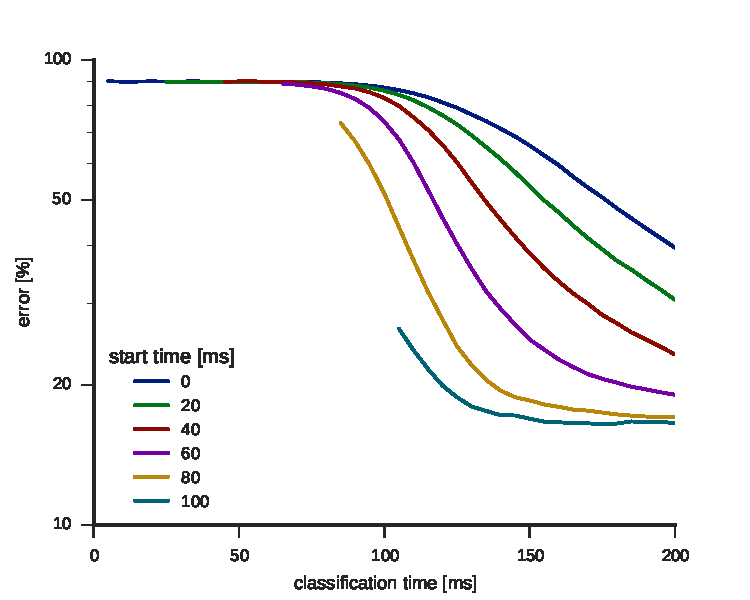
\includegraphics[width=0.4\columnwidth,clip=true,trim=2mm 0mm 10mm 8mm]{cifar10-lif-1628-200ms_pt-classplot.pdf} &
    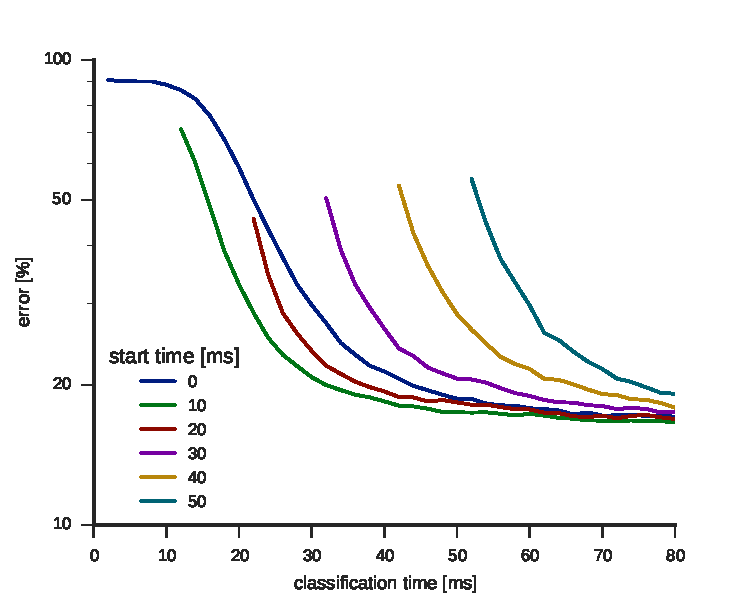
\includegraphics[width=0.4\columnwidth,clip=true,trim=2mm 0mm 10mm 8mm]{cifar10-lif-1628-80ms_pt-0ms_alpha-classplot.pdf} \\
    MNIST ($\tau_s = 2$ ms) & ILSVRC-2012 ($\tau_s = 0$ ms) \\
    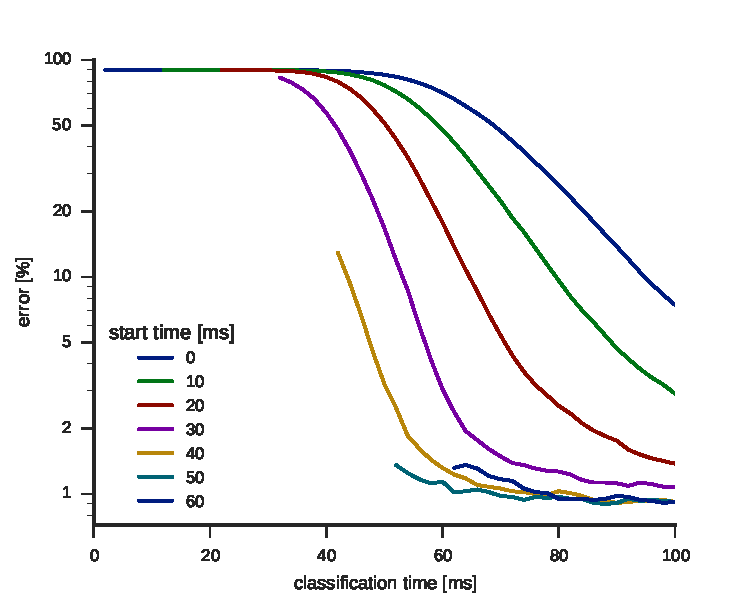
\includegraphics[width=0.4\columnwidth,clip=true,trim=2mm 0mm 10mm 8mm]{mnist-lif-0097-100ms_pt-2ms_alpha-classplot.pdf} &
    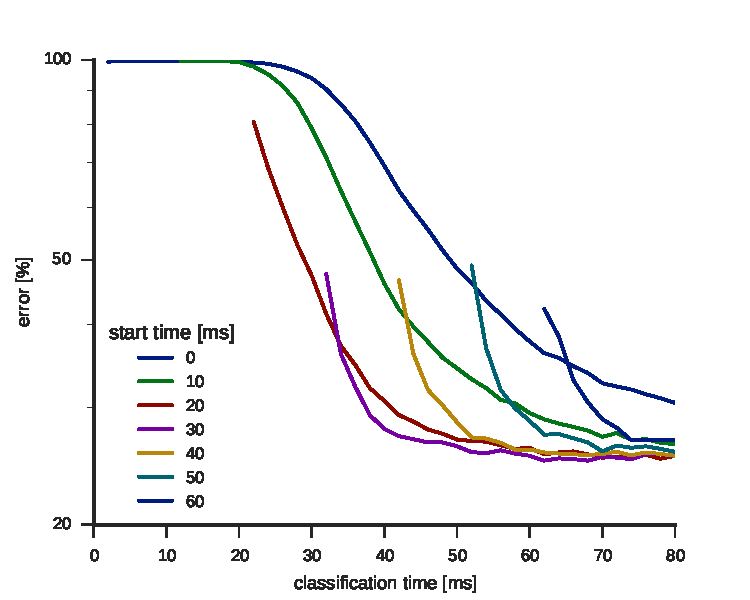
\includegraphics[width=0.4\columnwidth,clip=true,trim=2mm 0mm 10mm 8mm]{ilsvrc2012-lif-48-80ms_pt-0ms_alpha-classplot.pdf} \\
  \end{tabular}
  \captionb{Effects of classification time on accuracy.}{
    Individual traces show different starting classification times ($c_0$),
    and the x-axis the end classification time ($c_1$).
  }
  \figlabel{classtime}
\end{figure}

It is important to tune the classification time,
both in terms of the total length of time each example is shown for ($c_1$),
and when classification begins ($c_0$).
The optimal values for these parameters are very dependent on the network,
both in terms of the number of layers, firing rates, and synapse time constants.
\fig{classtime} shows how the classification time affects accuracy
for various networks.

%% Given that the CIFAR-10 network performs almost as well with no synapses
%% as with synapses,
%% one may question whether noise is required during training at all.
%% We retrained the CIFAR-10 network with no noise and ran with no synapses,
%% but could not achieve accuracy better than 18.06\% in the spiking network.
%% This suggests that noise is still beneficial during training.


\section{Discussion}

The soft-LIF neuron model is able to smooth the LIF rate response function,
such that it is differentiable and usable with backpropagation.
This smoothing technique is also applicable to other neuron models
with a static rate response function and a discontinuity in firing rate
around the firing threshold.
This could include the idiosyncratic neuron models
used on analog neuromorphic hardware \parencite[\eg/][]{Benjamin2014}.

With the soft-LIF model, the amount of smoothing can be adjusted so that
the model is arbitrarily close to the LIF model it is approximating.
This could allow for a relaxation over the course of training
where the soft-LIF model begins quite smooth
and then relaxes towards the actual LIF model,
so that there is no loss when changing to a LIF rate model.
In practice, I have not found that this is necessary.
Optimization tends to push neurons to be either robustly on or off,
particularly when noise is present either on the neural nonlinearity
or in the form of dropout.
This keeps neural inputs away from the firing threshold,
and thus out of the region where the soft-LIF and rate LIF models differ.

% Why does alpha noise model not work? Does not account for neuronal integration
The first noise model I developed for alpha synapses (model $\salpha$, \eqn{alpha-model})
did not perform well.
While this model perfectly characterizes
the variability of an alpha-filtered spike train,
it assumes that downstream neurons only receive an instantaneous snapshot
of the filtered spike train,
when in fact they integrate this spike train over time.
This leaky integration provides a second layer of filtering
on the incoming spike trains,
and is especially significant because the neural membrane time constant $\taurc$
tends to be much larger than the postsynaptic time constant $\taus$.
Without accounting for this filtering,
the model overestimates the amount of noise caused by spiking,
injecting too much noise during training resulting in lower accuracy.
Including the effects of this membrane filtering significantly improves performance.

% Discuss limitations of alpharc noise model
% - already discussed a bit above
% - two factors at play: rate of spikes and amplitude of spikes
%   (as determined by connection weights)
% Can illustrate this with alpharc_empirical.py
When accounting for neuronal integration,
the window over which a neuron is actually able to integrate
depends on its firing rate,
where the integration period is equal to the period between spikes
(minus the refractory period).
For example, a neuron that is firing quickly only integrates its inputs
for a short amount of time before it hits threshold and spikes,
whereas a neuron with a low firing rate
will require much more time to integrate before hitting threshold.
This is illustrated in \fig{alpharc-multineuron},
where the model correctly estimates the spiking variance for low
postsynaptic neuron firing rates,
but underestimates the spiking variance at high firing rates.
In the low firing rate case,
there is more time between spikes and thus
the full filtering effect of the membrane is able to be applied to most inputs;
thus the model---which includes the full membrane filter---does a good job.
As the firing rate increases,
the membrane has less time to filter inputs
and the effective filtering is reduced;
the model now overestimates the amount of filtering being applied to inputs,
thus underestimating the amount of variance in the output.

The firing rate of a neuron depends on the strength of its inputs,
which in turn depend on both the firing frequency and synaptic weighting
of each of its afferent neurons.
This dependence on both input frequency and weighting is important:
it means that to fully characterize the variability of a neuron's input signal,
one needs to transmit both these values for each afferent neuron.\footnote{
  This assumes that each of the input neurons is firing at constant rate,
  and that we are not interested in the phase of any neuron's firing.
  If a neuron's rate is variable (\eg/ a bursting neuron)
  then more values would be needed to fully characterize the variability.
  Similarly, if we are interested in neural phases
  (to account for synchrony between neurons),
  again more information would be needed.}
For example, if we only transmit a single value for each neuron
that is equal to its firing rate times synaptic weighting
(as is standard for rate-based networks),
then a downstream neuron cannot tell the difference
between a high-frequency input with a small weighting,
and a low-frequency input with a large weighting.
Yet, these two inputs have very different amounts of variance,
with a filtered high-frequency spike train
having much less variance than a similarly filtered low-frequency one.
The need for both the firing rate and synaptic weight of input neurons
can be seen in the Siegert model
for the rate of a LIF neuron with Poisson inputs \parencite{OConnor2013}:
it requires both values,
multiplying the weights times the rates to characterize the input mean,
and multiplying the squared weights times the rates to characterize the variance.

It is not theoretically difficult to transmit two values during training---%
or even more to characterize higher moments of the variability distribution---%
and the increase in training time would be
roughly proportional to the total number of moments transmitted
(\eg/ using two moments would take twice as computation in the forward pass
as a typical ANN, which uses only the mean).
Incorporating these values into the backwards pass would be more difficult,
since typical objective functions only constrain the mean firing rates
of the output units.
That said, even incorporating higher moments only in the forward pass
could be beneficial,
since these moments can affect the mean
(as seen in the Siegert model).
Current machine learning libraries are not designed to transmit
multiple values in this manner,
and would require significant modification.
Depending on the exact calculation required for the higher moments,
many of the basic computational elements such as convolution and pooling
may be able to be reused to compute the moments.

The alternative to accounting for such moments in a rate-based optimization method
is to simply switch to a spike-based optimization method.
Due to the relationship between first spike time and firing rate,
spike-based and rate-based methods are optimizing very similar quantities.
The main difference is that by accounting for individual spike times,
spike-based methods can better account for the inherent variability due to spikes.
Furthermore, they can exploit synchrony between neuron spike times,
information that is lost when dealing only in firing rates.
However, this ability to optimize the precise spike times of neurons
assumes that all neurons are starting
from the same resting state for each stimulus presentation.
Not surprisingly, all the networks I am aware of
that use spike-based optimization methods
do reset the system between stimulus presentations,
not only during training but also during testing.
If the system is run continuously, without resetting between presentations,
then much of the advantage of spike-based methods will disappear,
and I expect the two types of networks to perform similarly.
However, I am not aware of any such comparison in the literature.
The exception to this would be on dynamic stimuli,
such as those used by \textcite{Huh2017},
where spike times and synchrony over the course of a single stimulus are important.


%%  LocalWords:  DNNs CNNs cnns spikingmethods Gutig SpikeProp Bohte
%%  LocalWords:  LM Mostafa Stromatias ratemethods Carrasco Cao Diehl
%%  LocalWords:  Esser TrueNorth Merolla SVHN RBMs OConnor Siegert th
%%  LocalWords:  Neftci Eliasmith nef erf conv softlif lrrrr lifrate
%%  LocalWords:  lifraterho softrelusigma lifvariance alpharc minmax
%%  LocalWords:  ISI scn multineuron sgd multiview jittering un STDP
%%  LocalWords:  imagenet archmods Bergstra cifar noisemodels lrrrrr
%%  LocalWords:  synop synops esnn classtime Krizhevsky Levenberg OCL
%%  LocalWords:  Marquardt McKennoch Contrastive AlexNet FLOPs Kreutz
%%  LocalWords:  Manwani backprop Bekolay llr SNN essernote Zambrano
%%  LocalWords:  zamba llrrrrr img sota SNNs rrr cmpesser

\chapter{Biological Deep Learning}
\chplabel{learning}

The previous chapters of this thesis examined how spiking neural networks
of various depths might be implemented in a biological system.
They did not look at how a biological system might
\emph{learn} such networks.
This chapter looks at the problem of biological learning of deep networks,
specifically the following question:
How does the brain solve the spatial credit assignment problem
to develop deep networks skilled at solving real-world tasks?


\section{Background}

Recently, there has been increased interest from the machine learning community
as to how the brain might learn deep networks
(see \textcite{Marblestone2016} for a review).
One significant difference between these recent efforts
and many previous neuroscientific inquiries into learning
is the distinct emphasis on high-level functionality.
Machine learning researchers are accustomed to
evaluating their algorithms on functional tasks, such as object classification.
Their approach to biological learning is no different,
except that the learning algorithms are designed
to be biologically plausible.
This section first highlights the reasons why
the core of almost all state-of-the-art deep learning systems---%
the backpropagation algorithm---is not biologically plausible (\scn{bp-problems}).
Then, it reviews four ways to overcome this problem,
either by proposing neural mechanisms
that might be able to implement backpropagation (\scn{bp-biomechanisms}),
or by using alternative credit-assignment methods
that avoid the problems faced by backpropagation
(Sections~\scnref{fa-bg}, \scnref{dtp-bg}, and \scnref{ep-bg}).


\subsection{Biological problems with backpropagation}
\scnlabel{bp-problems}

The backpropagation algorithm (BP, see \scn{backprop})
has been very successful for training deep neural networks for many tasks,
including object classification.
Yet there are no known mechanisms by which the brain could implement BP.
\textcite{Bengio2015} list a number of factors
that make BP not biologically-plausible:
\begin{enumerate}
  \item \textbf{The weight transport problem:}
    BP uses the same connection weights
    both for the forwards pass (to perform inference)
    and the backwards pass (to transmit errors back through the network).
    Synapses in the brain are uni-directional,
    with a clear presynaptic and postsynaptic neuron.
    It is unclear how they could be used to transmit errors backwards.
    If a separate backwards connection is posited,
    its strength (connection weight) would need to be synchronized
    with that of the forward connection,
    again something that would be difficult in a biological system.
  \item \textbf{The derivative transport problem:}
    BP relies on the derivative of each hidden unit
    at the current operating point (forward activation).
    Not only is it unclear how this derivative might be computed,
    but it is then used to modulate the error signal,
    which is propagated further back in the network.
    Thus, each neuron needs to be able to use its derivative
    to modulate whatever mechanism is storing/transporting the error signal.
  \item \textbf{The linear feedback problem:}
    In BP, the feedback path is purely linear,
    whereas the biological neurons that would need to implement it are non-linear.
    This could potentially be addressed with population-coding methods
    like the NEF (see \scn{nef}),
    though care would have to be taken such that the number of
    required feedback neurons is within reasonable limits.
  \item \textbf{The spiking problem:}
    BP works with rate-based neurons, while the brain uses spiking neurons.
    While this problem has been partially addressed by the previous chapters
    of this thesis,
    it presents unique problems in the context of online learning,
    particularly since the derivative of a neuron is taken with respect
    to the firing rates (\ie/ filtered spikes), not the spikes themselves.
  \item \textbf{The timing problem:}
    The back-propagation phase of BP uses information
    from the forward-propagation phase.
    Not only is the output of the network used to compute the overall error,
    but both the presynaptic activity (used directly)
    and postsynaptic activity (used to compute the derivative at that node)
    are needed to update the weights.
    This is difficult in a biological deep network,
    because there is delay inherent in each neural connection.
    It takes a significant amount of time for information to propagate
    through the network to provide an output classification
    (which is presumably used to generate the error signal),
    and even more time for this error signal to be propagated back
    to the earliest layers.
    By this time, the activities of the early layers may have changed,
    putting them out of sync with the error signal.
  \item \textbf{The target problem:}
    Most of the success in machine learning for object classification
    has relied on a supervised learning paradigm.
    This assumes that for each training image,
    we know the true category label for that image.
    In the brain, it is not clear where this category label comes from.
    State-of-the-art DNNs learn from millions of images,
    but children only have to be told a handful of times what is a cat, dog, etc.
    The most obvious way for the brain to address this would be to combine
    large amounts of unsupervised learning
    with the small number of provided labels (supervised learning),
    for example to cluster similar input stimuli (\eg/ different cats)
    so that only the cluster has to be labelled, not all the individual stimuli.
    The details of how the brain might execute this semi-supervised learning
    are still largely unknown.
\end{enumerate}
Other than the term ``weight transport'',
which was coined by \textcite{Grossberg1987},
these problem names are first suggested here,
so they are not in common parlance.

One additional problem not pointed out by \textcite{Bengio2015}
is that BP networks do not obey Dale's principle \parencite{Baldi2016},
which states that neurons are almost always either excitatory or inhibitory,
meaning they only release either excitatory or inhibitory neurotransmitters,
not both.
In an abstract neural network,
this means that the signs of connections coming out of a neuron
should either be all positive or all negative, never a mix.
BP does not respect this rule,
and furthermore allows connections to change sign over the course of training,
which is also not biologically realistic.

Another problem not raised by \textcite{Bengio2015}
is how feedforward and feedback signals can combine within a single neuron
to simultaneously allow for feedforward prediction and learning \parencite{Guergiuev2017}.
In BP, there is an error signal associated with each hidden neuron,
determined by backpropagating the error signals of the previous layer
using the forward connection weights.
This error signal modulates learning at all of the afferent synapses of the neuron,
and thus must be injected into the neuron in some way.
The question is: How does this happen,
without mixing with the feedforward signals also entering the neuron?

A distinct but related problem is how the derivative of the neuron activity
might be propagated within the neuron to arrive at the synapses.
Significant research has been done in the area of \emph{backpropagating action potentials},
which are action potentials (spikes) that propagate from a neuron's soma
backwards through the dendrites \parencite{Waters2005}.
It is often hypothesized that these are related to learning,
but there is still a lack of understanding of how they operate,
and how they may propagate backwards without affecting or being affected by
the forwards activity of the dendrites.
These problems compound with the timing problem,
since not only does everything need to arrive in the right place,
it also has to be there at the right time.

In addition to these core problems with BP,
there are many additional problems related to the tools and techniques
typically used when training deep networks in machine learning.
I do not attempt to enumerate them all here,
nor do I address them in this thesis.
Examples include:
architectural problems, such as how neurons might implement
max-pooling or local contrast normalization (or something similar);
initialization problems, such as how connectivity between neurons
is initially established;
and training problems, such as how the brain could implement momentum,
or adjust learning rates
(at the network, layer, or individual neuron level, and possibly over time).
None of these features are necessary for deep learning---%
one can learn, to some degree, with a simple randomly or locally connected
network with no pooling, normalization, or momentum, and a fixed learning rate.
However, current state-of-the-art results in machine learning
typically combine many of these features.

The fundamental goal of this subfield, then,
is to determine how the brain solves the spatial credit assignment problem.
The first approach has been to propose biological mechanisms
by which BP itself could be implemented by the brain,
specifically by finding or positing biological mechanisms
to solve the weight transport problem
(since weight transport seems to be the largest problem with BP,
research has focused on addressing it).
The second approach is to look for alternative credit assignment methods,
again often starting with weight transport as the fundamental problem,
and once it has been solved,
expanding the method to address the other problems with BP as well.
A third approach is to reject the problem entirely,
by positing that the brain does not solve the credit assignment at all.
The new problem is then to explain how the brain might learn
to perform complex tasks
using only shallow supervised learning, unsupervised learning,
and other methods that do not rely on performing spatial credit assignment;
this lies outside the scope of this thesis.
Likely, the final answer will lie somewhere within all three of these approaches,
taking elements of BP and combining them both with
novel credit assignment strategies and other learning methods.


\subsection{Biological mechanisms for backpropagation}
\scnlabel{bp-biomechanisms}

\textcite{Bogacz2000} was one of the first papers to try to address
some of the biological plausibility limitations of BP.
The main contribution of the paper is that they perform a type of learning
with some similarities to BP
in a spiking neural network with a hidden layer.
However, their method is specific to a very constrained type of network.
The purpose of the network is to determine whether a stimulus is novel
or has been previously presented to the network (familiar).
If presented with a novel stimulus, the network updates
using a one-shot-learning paradigm so that the stimulus
will subsequently be classified as familiar.
The structure of this network has one hidden layer.
The connection weights from the input to the hidden layer are learned,
but the output neuron simply sums across the hidden neurons
and thresholds the response.
Credit assignment in this structure is much easier than in a general network,
since all hidden neurons contribute equally to the output,
while BP in a general network would need
to propagate the error backwards through variable connection weights
from the hidden neurons to the output.
The authors acknowledge this,
and identify the generalization to variable-weight outputs as future work.
This generalization (\ie/ solving the weight transport problem) is not straightforward,
and has been the focus of much of the subsequent work on
biologically plausible credit assignment.


\subsection{Feedback Alignment (FA)}
\scnlabel{fa-bg}

Feedback Alignment (FA) \parencite{Lillicrap2014}
is an alternative to BP for biological credit assignment.
The idea behind FA is that the feedback weights---%
the weights used to transmit error information backwards through the network---%
do not need to be the transpose of the feedforward weights ($W^T$),
as they are in BP.
Instead, FA uses random feedback weights,
and finds that the feedforward weights ``align'' themselves
so that useful error information can be propagated backwards through the network.
Specifically, the feedforward weights align themselves so that they are
not orthogonal to the feedback weights,
thus allowing the feedback error signals to push the neuron activities
in a direction that somewhat decreases the overall error
(despite not being the optimal, \ie/ gradient, direction).

% Poggio paper that says signs need to be the same
\textcite{Liao2015} focus on the weight transport problem,
and find that networks perform better when there is concordance between
the signs of the feedback weights and the feedforward weights.
This is perhaps not surprising,
since having feedback weights with the same signs as the feedforward weights
makes it highly likely that the two sets of weights will be far from orthogonal,
and thus the feedback weights will transmit useful information.
They also find that using some sort of batch normalization \parencite{Ioffe2015}
is very beneficial for any learning method where the feedback weights
are not the transpose of the feedforward weights
(which they broadly call ``asymmetric backpropagation'').
When training ANNs, weights may change sign during training,
so at first blush sign concordance may seem to not be biologically plausible,
since it could again require symmetry between feedforward and feedback weights
(albeit a more relaxed form of symmetry).
However, connections in the brain do not change sign over time;
they are all either inherently excitatory or inhibitory.\footnote{
  In fact, the constraint is even stronger:
  each \emph{neuron} only either has excitatory or inhibitory efferent connections.
  This is known as Dale's Principle.}
My conclusion is that sign changes over time do not pose a threat to possible
sign concordance in the brain,
though additional issues would have to be addressed
to concretely demonstrate its biological plausibility.
(I am not aware of a large-scale learning system
that obeys Dale's principle in the feedforward connections,
never mind one that would also obey both Dale's principle and sign concordance
in the feedback path.)

% Application of direct FA
\textcite{Nokland2016} uses FA to tackle some more difficult datasets---%
namely CIFAR-10 and CIFAR-100---as well as MNIST.
On MNIST, FA and its \emph{direct FA} variant (DFA, see \scn{fa-variants})
perform almost as well as BP across a number of different network architectures.
This paper also investigates a very deep network (with 100 layers of 240 tanh units each),
for which only DFA is able to converge,
presumably because it helps mitigate
the vanishing and exploding gradient problems.\footnote{
  However, the average test-set error (3.92\%) for this architecture
  is worse than for simpler architectures,
  including a 7-layer network (2.32\%)
  and a single-layer network with 800 tanh units (1.68\%).}
On CIFAR-10 and CIFAR-100,
FA and DFA are able to perform within a few percentage points
of BP on the test set for fully-connected networks.
For convolutional networks, FA and DFA perform significantly worse than BP
(27.1\% and 26.9\% vs 22.5\% respectively on CIFAR-10).
This could be because convolutional networks have fewer parameters,
meaning less redundancy,
and FA typically needs more parameters than BP
since the fixed random feedback weights
constrain the space that any particular neuron can explore during learning
(see \scn{fa-limitations-results}).
Finally, the paper introduces a novel FA variant called \emph{indirect FA},
which uses random direct feedback to the first hidden layer,
then forward connections to propagate this error forward (see \scn{fa-variants}).
There are some biological reservations to this approach, however,
since the forward connections skip the neural nonlinearity
and only use the connection weights.
No results from the IFA algorithm are presented.

\textcite{Baldi2016} perform more in-depth analyses on the FA algorithm,
both theoretical and experimental.
One of their key results is that FA is ``very robust
and works almost as well as BP'', and that
``performance is unaffected or degrades gracefully
when the the random backwards weights are initialized from different
distributions or even change during training.''
They perform experiments that look at varying levels of sparsity
in the feedback weights,
and find that FA achieves the same test error on MNIST
for sparsity levels from 20\% to 80\% (where non-zero elements all equal one).
Additionally, they test FA on a convolutional CIFAR-10 architecture,
and are able to achieve around 25\% test-set error
(their reference BP implementation achieves 16\%).
In addition to the tests on existing FA variants,
they introduce two novel FA variants,
which they call \emph{adaptive random backpropagation (ARBP)}
and \emph{adaptive skipped random backpropagation (ASRBP)}.
They operate the same as FA and DFA, respectively,
except that the feedback channels are also allowed to learn over time.
They do not perform extensive tests of these algorithms,
but a test on MNIST shows that ASRBP speeds up training slightly
as compared with its non-adaptive counterpart.
ARBP also works, but is much more fragile,
requiring a much smaller learning rate on the backwards connections,
and even then showing a non-smooth error trajectory.

\textcite{Neftci2017} implement a spiking version of direct FA
targeting neuromorphic hardware.
One major innovation over the \textcite{Lillicrap2016} spiking FA model
is that they do not use the exact neural derivative,
but rather use a surrogate derivative function
to approximate the neural derivative.
This allows them to train with LIF neurons.
They also introduce a form of probabilistic regularization
where spikes are randomly dropped based on a given probability;
this slightly improves test-set results.
The algorithm is event-driven,
meaning that weights are only updated when the corresponding presynaptic neuron spikes.
They demonstrate their spiking training method on MNIST,
and show that the final network can achieve 2.25\% test-set error.
Using a first-to-spike classification method yields around 4.5\% test-set error
while using 50 times less power than the better classification method.

\textcite{Samadi2017} also implement a spiking version of direct FA
(which they call broadcast alignment, or BA) in LIF neurons.
To approximate the LIF neuron derivative,
they fit the LIF rate-response curve with the following function:
\begin{align}
  f(x) = \max(0, c_1 \tanh(c_2 x)) \text{ ,}
\end{align}
where $x$ is the neuron input (current)
and $c_1$ and $c_2$ are arbitrary constants (hyperparameters).
This function fits the LIF rate-response curve reasonably well,
and is everywhere differentiable.
Using this as a surrogate derivative function,
they are able to train spiking networks to achieve 2.95\% test-set error on MNIST.
Their comparable rate-based networks achieve
1.40\% error with BP, 1.78\% with FA, and 2.36\% with DFA.


\subsection{Difference Target Propagation (DTP)}
\scnlabel{dtp-bg}

\newcommand{\vh}{\vect{h}}
%% $\hat \vh$

Difference Target Propagation (DTP) \parencite{Lee2015a}
is another algorithm for solving the spatial credit assignment problem
in a biological system.
Rather than using random feedback weights (as FA)
or symmetric feedback weights (as BP),
it \emph{learns} feedback weights to propagate error information.
The objective for the backwards path is to learn an approximate inverse $g^i$
for the forward function $f(\vh^{i-1}) = \vh^i = F^i(W^i \vh^{i-1})$
computed by the weights $W^i$ and neural nonlinearity $F^i$ at each layer.
Using this approximate inverse, we can compute a ``target'' value $\hat \vh^i$
for a layer given the target value $\hat \vh^{i+1}$ for the subsequent layer
\begin{align}
  \hat \vh^i = \vh^i + g^{i+1}(\hat \vh^{i+1}) - g^{i+1}(\vh^{i+1}) \text{ .}
  \eqnlabel{dtp}
\end{align}
This equation is designed so that when $\hat\vh^{i+1} = \vh^{i+1}$,
then $\hat\vh^i = \vh^i$.
This ensures that when there is no error at the highest layer,
then learning stops throughout the system.
The more intuitive choice of $\hat\vh^i = g^{i+1}(\hat\vh^{i+1})$---%
that is, simply propagating the target backwards---%
obeys this same property if $g^i$ is the inverse of $f^i$,
but not if $g^i$ is only an approximation of the inverse of $f^i$,
hence the choice of the more complicated \eqn{dtp}.
The target for the final layer is computed as a small step
in the direction of the gradient for that layer:
\begin{align}
  \hat \vh^N = \vh^N - \hat\eta \pdiff{O(\vh^N, y^*)}{\vh^N} \text{ .}
\end{align}
DTP can learn relatively deep networks;
the authors use it to learn a network with 7 hidden layers of 240 units each
on MNIST, achieving 1.94\% error using tanh units (compare 1.86\% for BP).
Interestingly, the same network with ReLU units
achieved 3.15\% with DTP, whereas BP achieved 1.62\%.
The authors also tested a network on CIFAR-10,
achieving 50.71\% with DTP versus 53.72\% for BP;
these numbers are good for a fully connected network without data augmentation.

% Towards deep learning with segregated dendrites
% - Explains how feedforward and feedback error can combine in one neuron
Although DTP offers a solution to the weight transport
and linear feedback problems,
it is unclear how exactly the feedback connections would operate
in a biological network.
There are two concerns:
1) each feedback connection is used to transmit two distinct values,
$g^i(\hat\vh^i)$ and $g^i(\vh^i)$,
it is unclear how they could be transmitted simultaneously;
2) the feedback connection $g^i$ needs to receive both
$\hat\vh^i$ and $\vh^i$ as input,
thus they must be stored in the same place,
but it is unclear how a single neural population
could store both feedforward ($\vh^i$) and feedback error ($\hat\vh^i$)
signals.
\textcite{Guergiuev2017} extend the DTP algorithm
with a compartmental neuron model,
addressing both of these questions.
Their hidden neurons have three compartments:
an apical dendrite that accepts feedback connections;
a basal dendrite that accepts feedforward connections;
and a soma, which receives input from both dendritic compartments
and controls the neuron's output.
There are two distinct phases to each stimulus presentation:
a forward phase, where the forward activity is computed;
and a target phase, where the correct category signal
is applied at the top layer.
This allows the model to compute ``plateau potentials'' $\alpha^f$ and $\alpha^t$
in the apical dendrites;
these signals are analogous to $g^i(h^i)$ and $g^i(\hat h^i)$
in DTP, respectively.
The output of each neuron is a firing rate,
determined by applying a sigmoid function to the soma's membrane voltage.
They demonstrate that a two-layer version of their model
is able to learn on MNIST,
achieving 3.2\% test-set error.


\subsection{Equilibrium Propagation (EP)}
\scnlabel{ep-bg}

Ten years ago, \textcite{Hinton2007} proposed the idea that
neurons could use derivatives in activity to transmit error information.
The general idea is that after the forward pass,
the top-level neurons in the network are perturbed
to push them closer to the target output values (as in DTP).
This change in activity over time codes for the error gradient of those neurons;
this is then propagated backwards
(using symmetric weights in Hinton's original proposition).
This would explain how neurons seemingly transmit both
forward signals and error information within a short span of time.
It could also help explain the spike-timing-dependent plasticity (STDP)
curves that \textcite{Bi1998} first identified empirically.

More recently, \textcite{Bengio2015} began to try to embody these ideas
into a quantitative model,
to demonstrate that they could actually work in practice.
This first paper presented a generative statistical model
utilizing the temporal derivative idea,
which was able to fill in corrupted sections of MNIST digits.

\textcite{Bengio2017} present an alternate use for the
derivative error encoding idea,
to perform inference in an energy-based model with symmetric weights.
They demonstrate that such a model reproduces STDP-like curves
in the weight changes.
\textcite{Scellier2017} extend this idea to a deep network
that is able to learn to perform the MNIST task,
achieving 0.0\% training error for all three networks tested
and between 2\% and 3\% test error depending on the number of layers used.
They title this algorithm Equilibrium Propagation (EP).
The model has two distinct phases:
an inference phase, where the model settles to a steady-state
given a stimulus;
and an error propagation phase,
where the energy is increased slightly based on the error of the network output,
and the model settles to a new steady-state minimizing
the combined energy from the stimulus and output error.
Weight changes are Hebbian,
based on the new (stimulus and label) steady-state activities,
and anti-Hebbian, based on the stimulus-only steady-state.
This pushes the model to associate lower energy
with the correct stimulus-label pairs.

This tentative connection between derivatives of neuron activity,
error, and STDP is very intriguing from a biological perspective,
since it would explain how neurons
are able to encode both activities for inference from the stimulus
and the error or correction information needed to learn.
The energy-based approach is also enticing,
since it quantitatively describes how an arbitrarily-connected neural system
can perform inference over time given a stimulus.
This opens the door for recurrent or lateral connections
that allow for a more complex inference process over time,
rather than just the simple feedforward inference used by
most current object-classification networks.\footnote{
  It also introduces more considerations,
  first and foremost the amount of time needed by a network
  with recurrent and lateral connectivity to settle to a steady-state.}
While these models do make these ideas more concrete,
there are still open questions about how they could work biologically.
The most significant one is again the weight transport problem;
the energy-based models re-introduce symmetric connections,
bringing back all the problems that other approaches
have explicitly worked to overcome.
While \textcite{Scellier2017} is hopeful that this can be overcome---%
making analogies to how autoencoders were able to move to using untied weights,
and how FA has addressed the need for symmetric weights in BP---%
it is still unclear how this might be addressed in an energy-based model.
The other biological consideration with these models is the timing aspect:
they involve distinct inference (no label information)
and clamped (label information provided) phases,
and in the case of \textcite{Scellier2017} these phases
are quite different lengths.
It is unclear how the brain might coordinate between such phases,
especially since the weight updates require neural activities
from both phases.

% - Could STDP be responsible for the anti-Hebbian/Hebbian switch, such that
%   the learning rule would only work properly when implemented in spiking neurons?
% - What about settling time? How could this be controlled?
% - Can this be combined with ideas from FA or DTP, such that symmetric back
%   weights are not required?
% - Can skip connections help reduce settling time? If I can get some class
%   information from the first hidden layer, this could help prime later layers


\section{Feedback Alignment}
\scnlabel{fa-methods}

Feedback Alignment (FA) is an alternative credit assignment method
first proposed by \textcite{Lillicrap2014};
since then, the core idea has been studied by a number of other researchers,
sometimes under the name Random Backpropagation (RBP) \parencite[\eg/][]{Liao2015,Baldi2016,Nokland2016}.

As mentioned in \scn{fa-bg},
the core idea of the algorithm is to use the same network structure as BP,
but to use static random feedback weights
(rather than the transpose of the forward weights)
during the backwards pass.\footnote{
  See \scn{backprop} for a presentation of the backpropagation (BP) algorithm.
  Some of the notation used in this section is defined there.}
This solves the weight transport problem,
since the feedback weights do not need to be kept identical to the feedforward ones.
Some variants of the algorithm (explored in \scn{fa-variants})
also address the derivative transport problem.
Finally, \textcite{Lillicrap2016} constructed a spiking version of their network
that also addresses the linear feedback, spiking, and timing problems
to varying degrees.

The success of the FA algorithm---%
and even the fact that it is able to learn anything at all---%
has surprised many researchers.
It seems counter-intuitive that back-propagating a random projection
of the subsequent layer's error
would transmit any useful information.
At first blush, it seems that the random projection would make the errors random:
uncorrelated to the output errors and thus uninformative and useless.
The first part of this intuition is correct:
the errors are in fact random.
However, since the random projections are fixed,
there is still structure to the errors,
and their values contain information about the nature of the output error.
To better understand how FA allows for learning,
it is important to develop intuitions about how the algorithm works.


\subsection{Intuitions}
\scnlabel{fa-intuitions}

% ``alignment'' intuition
% - Explain why this should happen. Hidden neurons are being pushed to be
%   selective for certain classes, so forward classification weights will match
The first intuition about FA is what I will call the ``alignment'' intuition.
It was presented as part of the original FA paper \parencite{Lillicrap2014},
and is where the name ``feedback alignment'' comes from.
The intuition is that over time, the forward weights in an FA network
will ``align'' themselves so they are not orthogonal with the backwards weights.\footnote{
  Here, two matrices $\mat A$ and $\mat B$ are essentially orthogonal
  if the images of these matrices across error vectors $\vect e$
  is approximately orthogonal:
  $\vect e \mat B \mat A^T \vect e^T \approx 0$ for all $\vect e$.
  In practice, FA works as long as $\vect e \mat B \mat W \vect e^T > 0$
  for most error vectors $\vect e$,
  where $\mat W$ is our forward weight matrix
  and $\mat B$ is our random feedback weight matrix \parencite{Lillicrap2014}.
  To assess this, we can look at the eigenvalues of $\mat B \mat W$:
  if they all have positive real components,
  then the dot product in the previous expression will be positive for all $\vect e$.}
If the forwards and backwards weights are orthogonal,
then the projected error will not provide any useful information
to help correct the actual errors of the network.
Put another way, the change in the network weights
will be orthogonal to the gradient,
and thus not decrease the error.\footnote{
  It is important to note that this explanation assumes linear neurons,
  but the same ideas apply in the case of nonlinear neurons.}
As soon as the feedback weights are non-orthogonal (in a positive direction)
with the feedforward weights,
then each update will move at least partially in the same direction as the gradient,
that is, in a direction that decreases the error.
The smaller the angle between the feedforward and feedback weight matrices,
the more similar the update is to the gradient,
and the more the error will decrease with each step.
If the angle is zero, then the feedback weights are the transpose of the feedforward,
and we move in the direction given by BP.
\textcite{Lillicrap2014} presented this as the motivating idea behind FA,
and found empirically that in an FA network,
the angle between the feedforward and feedback matrices
reduces to much less than 90\degree/ (typically less than 45\degree/ in their networks).

So why does this ``alignment'' happen?
To explain this, I introduce a second intuition:
the random feedback matrices push each hidden neuron
to be selective to certain classes and not others.
For example, for the final hidden layer,
each neuron has a randomly-weighted feedback connection to each output error neuron.
If a neuron happens to have a strong positive feedback connection to class A,
then each time a stimulus of class A is presented but not correctly classified
(such that the output error is large),
then that neuron will be pushed to be more active.
It thereby develops an affinity for stimuli of class A.
The reverse process can happen if the neuron has a strong negative connection
to class B; the neuron will learn to be silent for class B stimuli.
Thus, the neuron develops a selectivity for some classes over others.
Once this selectivity begins to form,
then the \emph{feedforward} connections
between that neuron and those classes will strengthen,
since activity in that neuron is indicative of those classes.
In this manner, the neuron will develop both strong positive feedback
and feedforward connections for some classes,
and strong negative ones for other classes.
This makes the feedforward weights more similar to the feedback weights,
causing them to align.

A third intuition is that this push for class selectivity
only happens when there is error in the network output.
An error causes neurons to learn to respond more strongly to the problematic stimulus.
The most change occurs for neurons with a significant derivative
at their current activity level,
since this derivative modulates the learning (see \scn{fa-variants}).
The initial forward connections in the network are random,
and thus some neurons are slightly predisposed from the start
to respond to some stimuli over others.
These factors, when combined with the random feedback weights,
result in hidden neurons that learn to form distributed representations
across all classes and stimuli in the dataset.
Different neurons are responsible for different classes,
and different groups of stimuli within a class.


\subsection{Variants}
\scnlabel{fa-variants}

\begin{figure}
  \centering
  \tikzstyle{line} = [draw]

\begin{tabular}{c|c|c}
  GFA & LFA & DFA \\
\begin{tikzpicture}[->,>=stealth',auto,node distance=2cm,
    thick,circnode/.style={circle,draw,inner sep=2,minimum size=1cm}]

  \node[circnode] (h) {$h^n$};
  \node[circnode] (ha) [above of=h] {$h^{n+1}$};
  \node[circnode] (hb) [below of=h] {$h^{n-1}$};
  \node[circnode] (e) [right of=h, node distance=2.5cm] {$e^n$};
  \node[circnode] (ea) [above of=e] {$e^{n+1}$};
  \node[circnode] (eb) [below of=e] {$e^{n-1}$};

  \path[line] (hb) -- node [right] (Wb) {$W^n$} (h);
  \path[line] (h) -- node [right] (Wa) {$W^{n+1}$} (ha);
  \path[line] (ea) -- node [right] (Ba) {$B^{n+1}$} (e);
  \path[line] (e) -- node [right] (Bb) {$B^n$} (eb);

  \path[line] (h) -- node {$h'$} (e);
  \path[line] (ha) -- node {$h'$} (ea);
  \path[line] (hb) -- node {$h'$} (eb);
  %% \path[line] (h) to [out=30,in=150] node {$h'$} (e);
  \path[line] (ea) to (Wa);
  \path[line] (e) to (Wb);

  \node[] (h0) [below of=hb, node distance=10mm] {};
  \node[] (h1) [above of=ha, node distance=10mm] {};
  \path[line] (h0) -- (hb);
  \path[line] (ha) -- (h1);
  \node[] (e0) [below of=eb, node distance=10mm] {};
  \node[] (e1) [above of=ea, node distance=10mm] {};
  \path[line] (e1) -- (ea);
  \path[line] (eb) -- (e0);
  \node[] (h00) [right of=h0, node distance=10mm] {};
  \path[line] (eb) -- (h00);
\end{tikzpicture}
&
\begin{tikzpicture}[->,>=stealth',auto,node distance=2cm,
    thick,circnode/.style={circle,draw,inner sep=2,minimum size=1cm}]

  \node[circnode] (h) {$h^n$};
  \node[circnode] (ha) [above of=h] {$h^{n+1}$};
  \node[circnode] (hb) [below of=h] {$h^{n-1}$};
  \node[circnode] (e) [right of=h, node distance=2.5cm] {$e^n$};
  \node[circnode] (ea) [above of=e] {$e^{n+1}$};
  \node[circnode] (eb) [below of=e] {$e^{n-1}$};

  \path[line] (hb) -- node [right] (Wb) {$W^n$} (h);
  \path[line] (h) -- node [right] (Wa) {$W^{n+1}$} (ha);
  \path[line] (ea) -- node [right] (Ba) {$B^{n+1}$} (e);
  \path[line] (e) -- node [right] (Bb) {$B^n$} (eb);
  \path[line] (ea) to (Wa);
  \path[line] (e) to (Wb);

  \node[] (h0) [below of=hb, node distance=10mm] {};
  \node[] (h1) [above of=ha, node distance=10mm] {};
  \path[line] (h0) -- (hb);
  \path[line] (ha) -- (h1);
  \node[] (e0) [below of=eb, node distance=10mm] {};
  \node[] (e1) [above of=ea, node distance=10mm] {};
  \path[line] (e1) -- (ea);
  \path[line] (eb) -- (e0);
  \node[] (h00) [right of=h0, node distance=5mm] {};
  \path[line] (eb) -- (h00);

  \path[line] (h.east) .. controls +(right:7mm) and +(up:5mm)
                        .. node [above right] {$h'$} (Wb.north);
  \path[line] (ha.east) .. controls +(right:5mm) and +(up:5mm)
                        .. node [above right] {$h'$} (Wa.north);
  \path[line] (hb.east) .. controls +(right:5mm) and +(up:5mm)
                        .. node [above right] {$h'$} (h00.north);
\end{tikzpicture}
&
\begin{tikzpicture}[->,>=stealth',auto,node distance=2cm,
    thick,circnode/.style={circle,draw,inner sep=2,minimum size=1cm}]

  \node[circnode] (h) {$h^n$};
  \node[circnode] (ha) [above of=h] {$h^{n+1}$};
  \node[circnode] (hb) [below of=h] {$h^{n-1}$};
  \node[circnode] (e) [right of=h, node distance=2.5cm] {$e^n$};
  \node[circnode] (ea) [above of=e] {$e^{n+1}$};
  \node[circnode] (eb) [below of=e] {$e^{n-1}$};
  \node[circnode] (es) [right of=e, node distance=2cm] {$e^*$};

  \path[line] (hb) -- node [right] (Wb) {$W^n$} (h);
  \path[line] (h) -- node [right] (Wa) {$W^{n+1}$} (ha);
  \path[line] (es) -- node [above right] (Bc) {$B^{n+2}$} (ea);
  \path[line] (es) -- node [below] (Ba) {$B^{n+1}$} (e);
  \path[line] (es) -- node [below right] (Bb) {$B^n$} (eb);

  \node[] (h0) [below of=hb, node distance=10mm] {};
  \node[] (h1) [above of=ha, node distance=10mm] {};
  \path[line] (h0) -- (hb);
  \path[line] (ha) -- (h1);
  \node[] (h00) [right of=h0, node distance=5mm] {};

  \path[line] (ea) to (Wa);
  \path[line] (e) to (Wb);
  \path[line] (eb) -- (h00);

  \path[line] (h.east) .. controls +(right:7mm) and +(up:5mm)
                        .. node [above right] {$h'$} (Wb.north);
  \path[line] (ha.east) .. controls +(right:5mm) and +(up:5mm)
                        .. node [above right] {$h'$} (Wa.north);
  \path[line] (hb.east) .. controls +(right:5mm) and +(up:5mm)
                        .. node [above right] {$h'$} (h00.north);
\end{tikzpicture}

\end{tabular}

  \captionb{Diagrams of the three main variants of FA.}{
    Global-derivative FA (GFA, left) has an identical structure to BP,
    but replaces the transpose weights with random weights: $(\mat W^n)^T \to \mat B^n$.
    Local-derivative FA (LFA, middle) is similar to GFA,
    but only applies the neuron derivatives $h'$ locally.
    Direct FA (DFA, right) projects the error signals
    directly from the output error $e^*$.
    Since both the LFA and DFA feedback pathways are linear,
    feedback matrices $\mat B$ can be chosen such that they are equivalent.
  }
  \figlabel{fa-variants}
\end{figure}

There are a number of different variants of the FA algorithm,
as mentioned in \scn{fa-bg}.
For all the variants, the structure of the weight update is the same:
\begin{align}
  \Delta W^n_{ij} &= -\eta e_j^n f'(a_j^n) h_i^{n-1} \text{ .}
\end{align}
That is, all variants use the activity of the presynaptic neurons $h_i^{n-1}$,
the derivative of the postsynaptic neuron activity $f'(a_j^n)$,
and a modulatory error signal $e_j^n$ (and the learning rate $\eta$).
Additionally, the output layer performs shallow learning in all variants,
as in BP:
\begin{align}
  \Delta W^{N+1}_{ij} = -\eta e^*_j h_i^N
\end{align}
where $e^*_j = y_j - y^*_j$ and $N$ is the number of hidden layers in the network.
What changes between variants is how the feedback error signal $\vect e^n$
is determined,
that is, the structure of the feedback chain.
\fig{fa-variants} shows diagrams of the three main variants
examined in this thesis.

The original FA algorithm from \textcite{Lillicrap2014}
uses the neuron derivatives as part of the feedback chain;
I call this \emph{global-derivative FA} (GFA).
Its key feature is that it uses the hidden-neuron derivatives in the feedback chain:
\begin{align}
  e^n_j = \sum_q e^{n+1}_q f'(a^{n+1}_q) B^{n+1}_{qj} \text{ .}
\end{align}
Here, $\mat B^{n+1}$ is the matrix of random feedback weights
that projects the error from the space of layer $n + 1$ to the space of layer $n$.\footnote{
  All variants of FA include random feedback weight matrices $\mat B$,
  though the dimensionality of the matrices may differ between variants.}
Therefore, the update to the weights $W^n_{ij}$
depends not only on the local postsynaptic derivative $f'(a_j^n)$,
but also on the hidden neuron derivatives from all subsequent layers
(where the exact dependence is determined by the connectivity of the $\mat B$ matrices).

The first variant removes the neuron derivatives from the feedback chain,
and only uses each derivative locally for updating the weights
going into the corresponding neuron.
I call this \emph{local-derivative FA} (LFA);
it can be formulated as follows:
\begin{align}
  e^n_j = \sum_q e^{n+1}_q B^{n+1}_{qj} \text{ .}
\end{align}

The second variant---\emph{direct FA} (DFA)---builds off the fact that
the local-derivative FA passes the error signal at the classification layer $\vect e^*$
through subsequent random linear projections to produce $\vect e^n$.
Assuming no layer has fewer hidden neurons
than the number of output dimensions of the network
(such that no information is lost about $\vect e^*$),
we can achieve a very similar effect by simply projecting each layer's error
signal randomly off the output error signal:
\begin{align}
  e^n_j = \sum_l e^*_l B^{n+1}_{lj} \text{ .}
\end{align}
This variant was proposed both by \textcite{Lillicrap2016} and \textcite{Nokland2016}.
It is also explored by \textcite{Baldi2016},
who call it \emph{skipped random backpropagation}.

A third variant---called \emph{indirect FA} (IFA)---was proposed by \textcite{Nokland2016}.
They present this variant in the context of a two-hidden-layer network.
The first hidden layer receives random feedback from the output layer,
just as with DFA:
\begin{align}
  e^1_i = \sum_l e^*_l B^*_{li} \text{ .}
\end{align}
The second hidden layer's error is based on that of the first layer,
using the input weights of the second layer:
\begin{align}
  e^2_j = \sum_i e^1_i W^2_{ij} \text{ .}
\end{align}
While perhaps somewhat interesting theoretically,
there are reasons to have reservations about using it as a biological model.
The main reservation is that it uses the connection weights
between the first and second hidden layers ($\mat W^2$),
but the error $\vect e^1$ that is projected through these weights
is not integrated by the second hidden-layer neurons
(\ie/ their activity is not affected),
and conversely the error signal is not affected by the neural nonlinearity.
The neuron would need some mechanism such that the error signal
only reaches the synapses and is not passed on to the soma,
while the feedforward currents---passing through the same synapses---%
would pass through to the soma as usual.
Since there is no mechanism to distinguish between electrical currents
in this manner, this poses a significant problem with this method.\footnote{
  The problem of how to manage feedforward and error signals in the same
  cell is common to all variants of Feedback Alignment,
  and learning more generally.
  However, in the other variants,
  feedforward and error signals would only
  co-occur in the postsynaptic neuron's dendrites,
  and would not require passing error information from
  the presynaptic neuron to the postsynaptic neuron through synapses,
  as required by IFA.}
Additionally, it is unclear how this method would generalize
to more than two hidden layers.
If we were to use the third hidden layer's weights to project $\vect e^2$,
then we again run into the problem that we are making use
of the second layer's synapses while avoiding the neural nonlinearity.
Due to these reservations,
combined with the fact that \textcite{Nokland2016}
provided no advantages for the IFA variant,
this thesis does not examine IFA any further.

It is also possible to have learning in the backwards channel,
called \emph{adaptive} FA.
\textcite{Baldi2016} introduce weight changes for their backwards weights
that are proportional to the product of the forward activities
for the layer in question,
as well as the randomly projected error for the previous layer:
\begin{align}
  \Delta B^n_{ij} = \eta\mu \delta^n_i h^{n-1}_j
\end{align}
where $\delta^n_i = e^n_i f'(a^n_i)$,
$\eta$ is the learning rate for the forward weights,
and $\mu$ is a scaling factor on $\eta$ to determine the feedback learning rate.
This is the same update as is applied to the forward weights;
for that reason, I will call it \emph{symmetric} adaptive FA.
A similar update can be applied to DFA:
\begin{align}
  \Delta B^n_{lj} = \eta\mu e^*_l h^{n-1}_j \text{ .}
\end{align}
The idea of adaptive FA is intriguing,
since it can potentially allow initially random feedback weights
to better align with the forward weights,
resulting in better error information transmission
and therefore faster convergence and better performance.
It may also increase the biological plausibility of the model,
since it is unclear whether the brain could maintain static feedback connections
over long periods of time,
particularly when the adjacent forward connections are learning.
In the case of symmetric adaptive FA,
it does also raise the biological question
as to how the forward activities come to modulate the backwards weights.
\textcite{Baldi2016} present only preliminary results on adaptive variants
of both GFA and DFA,
but find that in the case of DFA,
adding adaptation improves convergence and overall performance,
whereas introducing it to GFA makes the algorithm unstable
(even for $\mu = 0.1$).

I am not aware of any other published investigations
into adaptive variants of FA.
Here, I propose two new adaptive variants based on Hebbian learning:
one using a pure Hebbian learning rule;
and the other using Oja's rule \parencite{Oja1982},
a more stable variant of Hebbian learning.
These adaptive variants can be viewed as unsupervised forms of adaptation,
whereas symmetric adaptive FA is more like supervised learning
(where the forward path is providing the teaching signal).
Hebbian ADFA is given by:
\begin{align}
  \Delta B^n_{lj} = \eta\nu e^*_l e^{n-1}_j
\end{align}
where $\eta$ is the forward learning rate
and $\nu$ is a scaling factor on this learning rate.
Oja ADFA is given by:
\begin{align}
  \Delta B^n_{lj} = \eta\nu \left[
    e^*_l e^{n-1}_j - \beta B^n_{lj} \left(e^{n-1}_j\right)^2 \right]\text{ ,}
\end{align}
where $\beta$ is a scaling parameter
to control the amount of regularization (often just set to unity).
These adaptation rules can be combined with symmetric ADFA
to create hybrid rules:
Symmetric Hebbian (Symm-Hebb) ADFA;
and Symmetric Oja (Symm-Oja) ADFA.
These learning rules use a linear weighting of the $\Delta\mat B$ updates
\begin{align}
  \Delta\mat B^n_\text{Symm-Hebb} = &
    \eta\mu \Delta\mat B^n_\text{Symm} + \eta\nu \Delta\mat B^n_\text{Hebb} \\
  \Delta\mat B^n_\text{Symm-Oja} = &
    \eta\mu \Delta\mat B^n_\text{Symm} + \eta\nu \Delta\mat B^n_\text{Oja} \text{ .}
\end{align}
Typically, we will have $\mu = 1$ and $\nu = 0.1$,
giving more weight to the ``supervised'' portion of the rule.


\subsection{Comparison of variants}

Given these three different implementations of the FA algorithm
(GFA, LFA, and DFA),
how should we choose which one to use?
There are two key considerations: performance and biological plausibility.
In \scn{fa-variants-results},
I compare the performance of the different variants,
and find that all the variants perform similarly,
with perhaps the direct variant performing slightly better.

In terms of biological plausibility,
we must consider both how the neuron derivatives are used
and how the error is transmitted.
The neuron derivatives can either be used locally or globally,
and it is not entirely clear for either case
what mechanisms the brain might use to compute these derivatives.
However, with mechanisms such as backpropagating action potentials
being proposed for transmitting information about postsynaptic neuron activity
back to the synapse \parencite{Waters2005},
it is not a stretch to imagine how such a mechanism could also transmit
derivative information to the synapse,
perhaps computing the derivative in the dendrites.
How the neuron derivative could be computed or transmitted
outside of the neuron and its dendritic arbour is harder to imagine,
and this is what would be needed to transmit the derivative globally.
That said, in \scn{learning-derivatives} I will explore using alternatives
to the neuron derivative itself in the computation (\ie/ surrogate derivatives),
including functions as simple as a step function
that turns on learning when the postsynaptic neuron is active
and turns it off otherwise.
It is easier to imagine how a simpler function like this
could be computed or transmitted outside of the postsynaptic neuron.
My conclusion from this exploration is that,
in the variants that only use the derivative locally (\ie/ LFA and DFA),
it seems easier for a biological system to implement the necessary
derivative computations.
Nevertheless, it may be possible for a biological system to implement
the computation involved in GFA, if necessary.

As for error transmission,
direct FA as it has been presented---%
where all the neuron error signals are direct random projections
from the output error---%
is not biologically plausible for the simple reason
that it would require too many long-range connections for each hidden neuron
to have projections back to the higher visual cortices.
However, this problem can be solved
by assuming there are copies of the output error
in the earlier visual cortices.
Making these copies would be quite feasible using a population-coding scheme
such as is used by the NEF.
This would require a more modest number of long-range connections,
and each hidden neuron could then receive random projections
from this local copy of the error signal.
The connections required by direct FA are thus not implausible
assuming that they are organized in such a way that they are predominantly local.
Ensuring sparse connections between populations would further help
the plausibility of the model by again decreasing the long-range connections.

With the other FA variants (GFA and LFA),
the biological plausibility of their connection structure
is determined mainly by how sparse they are.
These feedback connection matrices should obey the same constraints
as feedforward connection matrices do.
For example, if a model has sparse feedforward connections for biological reasons,
then the structure of the feedback connections should also be relatively sparse.

Another problem faced by all the FA variants---if implemented in a biological system---%
is how to backpropagate a linear error using nonlinear neurons
(the \emph{linear feedback problem}).
The core of the problem is that neural firing is non-negative,
whereas the error signals (whether in the output space or the randomly projected space)
have both positive and negative components.
An additional aspect to the problem is that the input-output relationship
of the neuron is nonlinear even in the firing regime,
meaning that the error in a particular dimension could not be decoded linearly
even using two neurons (an ``on'' and an ``off'' neuron)
to represent that dimension.
One partial solution that still allows one neuron per error dimension
is to simply shift all the error signals so that they are non-negative
(perhaps clipping or squashing some very negative components
using a function like \textrm{tanh}).
This corresponds to having a non-zero level of neural activity
represent zero error,
and is the approach taken by \textcite{Lillicrap2016}
in their spiking implementation.

Using population coding is another way to address the linear feedback problem,
and works quite well when there are relatively few error dimensions.
This is often the case in DFA, specifically when we have few output categories.
In the case of GFA and LFA,
the number of error dimensions corresponds to
the number of hidden neurons in the layer
for the intermediate (\ie/ non-output) error signals.
Thus, for these variants, population coding would require
multiple feedback neurons for each feedforward neuron
(a minimum of two just to represent the positive and negative error components,
and upwards of ten to remove some of the significant effects of the neural
nonlinearities in the error encoding).
This is likely to lead to an explosion in the number of neurons
required to implement the network.


\subsection{Parameters}
\scnlabel{fa-parameters}

For the most part, FA shares the same parameters and hyperparameters as BP.
The main difference is that FA does not constrain the backwards weights.
Whether one should consider these as parameters or hyperparameters is unclear;
like hyperparameters, they are arbitrary and are not adjusted
as part of the learning procedure (except in adaptive FA variants),
but like parameters, there are many of them,
and they are similar in their biological interpretation to the forward weights,
which are clearly parameters.
Also, one would hope that the performance of FA is not dependent
on their specific values.
Thus, I prefer to look at the backwards weights $B$ as parameters,
but view the distribution from which they are randomly drawn as a hyperparameter.
The original work by \textcite{Lillicrap2014} used Gaussian distributed weights,
and most derivative works have followed suit.
Yet there are many possible choices for the distribution of the feedback weights.
\textcite{Baldi2016} explores some of these alternatives,
looking at the sparsity of feedback weight matrices.

To simplify the discussion, I consider the distribution of the weights
for a single neuron in the context of DFA,
where each neuron has a weight connecting it to each of the output class errors.
This weight represents how the neuron in question responds
to errors in that class.\footnote{
  A positive error for a particular class output
  means that the network is outputting that class,
  but the correct label corresponds to a different class (the output is too high).
  A negative error means that that output dimension corresponds to the correct class,
  and the network is not outputting it strongly enough (the output is too low).
  Noting the effects of these error signs,
  and observing that the weights are modified in the negative direction
  of the error gradient,
  one can derive the correspondences between weight sign
  and neuron behaviour.}
A positive weight means the neuron will increase
its activity if the correct label is of the corresponding class,
but the network is not classifying it as such.
Furthermore, it will decrease its activity if the error is positive,
meaning it will try to be less active when the network
is falsely responding to the corresponding class.
Together, this will push the neuron to be selective
for the class with a positive weight.
A negative weight means that the neuron will become less active
if the error is negative, and more active if it is positive.
This will push the neuron to be less active for examples of the class in question,
and more active when examples of other classes are shown
but are misclassified as this class,
resulting in a neuron whose activity indicates the stimulus is \emph{not}
the class in question.
A weight of zero means that a neuron will not update itself
based on errors in a particular class,
but the neuron can still develop correlations or anti-correlations
with stimuli of that class
as a by-product of updating itself based on other class errors.

A distribution of backwards weights can therefore be classified partly in terms of
how many positive, negative, and zero values it contains.
A \emph{sparse} distribution results in many weights that are zero,
whereas a \emph{dense} distribution results in weights that are all non-zero.
Distributions can also be classified by their variance
within positive and negative values.
For example, a Gaussian distribution ($w \sim N(0, 1)$) and binary distribution ($w \in \{-1, 1\}$)
are both dense distributions with the same (expected) number
of positive and negative values,
but the Gaussian distribution will yield large and small weights,
whereas in the binary distribution all weights have the same magnitude.

% discuss flexibility provided by feedback weight magnitudes
%  This can help get around the vanishing (and exploding) gradient problems.
%  It is also another hyperparameter that needs to be determined, as it
%  essentially sets the learning rate for earler layers.
%  We may want this to be smaller for early layers, or equal for all layers.
%  This parameter can also be used to make FA appear better than BP by
%  having it learn more quickly initially.
%  In some ways, this is a true benefit, because the magnitude of the feedback
%  and therefore weight updates is not tied to the forward weight magnitude.
%  On the other hand, it can be used to make FA appear better than BP as in
%  Lillicrap2016 Figure 3d
%  Another possible advantage is that the feedback is not dependent
%  on the feedforward weight magnitudes. In BP, if initial weight magnitudes
%  are too small, initial learning can progress too slowly.
A final aspect of the feedback weights is their magnitude.
In BP, the magnitude of the feedback weights is determined
by the feedforward weights (since they are the same).
If the forward weights in any layer are too small,
then the preceding layers will have very small gradients,
and if they are too large, then the gradients will also become large;
this is the basis of the vanishing and exploding gradient problems.\footnote{
  In deep networks, these problems compound when many layers in a row
  have weights that are too small or too large.
  Thus, the vanishing and exploding gradient problems are typically discussed
  in the context of deep networks,
  or recurrent networks when backpropagation-through-time is used
  (since these are equivalent to deep networks with tied weights between layers).}
FA can avoid these problems since the magnitudes of the backwards weights
are independent of those of the forwards weights.
The weight magnitudes are redundant with the learning rates,
since both control the rate of learning at a particular layer.
This also means that one must take care when comparing FA and BP results directly,
since the combination of initial weight magnitudes, learning rates,
and feedback weight magnitudes can have significant effects.
For example, some applications of FA show the algorithm
learning faster than BP \parencite[\eg/][Figure 3d]{Lillicrap2016},
but this is simply an artifact of using large feedback weight magnitudes
resulting in a better effective learning rate for FA.


\subsection{Neuron derivatives}
\scnlabel{learning-derivatives}

Like BP, FA makes use of
derivatives of the neuron rate response functions.
These derivatives quantify how much each neuron's firing rate will change
in response to a small change in its input current;
thus, the derivative for each neuron is evaluated at that neuron's activity level,
as determined by the feedforward pass.

As described at the start of the previous chapter,
there is no clear way to take the firing rate derivative of a spiking neuron
based on the spiking output.
This is because the instantaneous firing rate can only be estimated
from the output spikes,
and thus the derivative will also be an estimate.
We have additional problems with LIF neurons,
because the firing rate derivative, even if we could take it,
is not well behaved (it has a singularity at the firing threshold).
To avoid using the actual derivative of the LIF rate response curve,
one option \parencite{Neftci2017,Samadi2017}
is to use an alternative or ``surrogate'' function
in place of the actual derivative.
The goal is to choose surrogate functions that are close enough
to the actual derivative such that learning still proceeds well,
but without any of the instabilities caused by the singularity
in the LIF derivative function.
This is the same motivation as for the soft-LIF neuron model
introduced in \scn{softlif}.

Theoretically, the most important characteristic
of a surrogate derivative function
is that it has the same sign as the actual derivative it is standing in for.
I will show here that if the sign of the surrogate derivative
matches that of the actual derivative for all inputs,
then the error will continuously decrease
when training with BP (with an infinitesimally small step size).
Consider a hidden layer in a network $h_j \equiv f\left(\sum_i x_i W_{ij}\right)$.
We wish to determine how the cost changes as we adjust the weights.
The change in the objective function (cost) for a given change in weight is
\begin{align}
  \pdiff{O}{W_{ij}} &= \pdiff{O}{h_j} \pdiff{h_j}{W_{ij}} \\
    &= e_j f'_j x_i
\end{align}
where $e_j \equiv \pdiff{O}{h_j}$ and $f'_j \equiv f'\left(\sum_i x_i W_{ij}\right)$.
In ordinary BP, we adjust the weights in the opposite direction
of this gradient in order to minimize the cost:
\begin{align}
  \diff{W_{ij}}{t} &\propto -\pdiff{O}{W_{ij}} \\
    &= -e_j f'_j x_i \text{ .}
\end{align}
When training with a surrogate derivative,
we replace the $f'_j$ term with a $g_j \equiv g(\sum_i x_i W_{ij})$ term.
We can derive how the cost changes over time in our network:
\begin{align}
  \diff{O}{t} &\propto \pdiff{O}{W_{ij}} \diff{W_{ij}}{t} \\
    &= \left(e_j f'_j x_i\right) \left(-e_j g_j x_i\right) \\
    &= -e_j^2 x_i^2 f'_j g_j \text{ .}
\end{align}
If $f'_j$ and $g_j$ always have the same sign,
then this expression is non-positive
and the cost will always decrease.
Thus, we need our surrogate derivative function
to have the same sign as our actual derivative function to maintain stability.
Note that this is not a sufficient condition for stability,
only a necessary one.
BP with a non-infinitesimal learning rate is always potentially unstable,
with more risk of instability the larger the learning rate becomes.
Even if two surrogate derivative functions both match the sign
of the actual neuron derivative,
one may become unstable more quickly than the other
as the learning rate increases.
I explore this question empirically in \scn{fa-derivatives-results}.


\begin{figure}
  \centering
  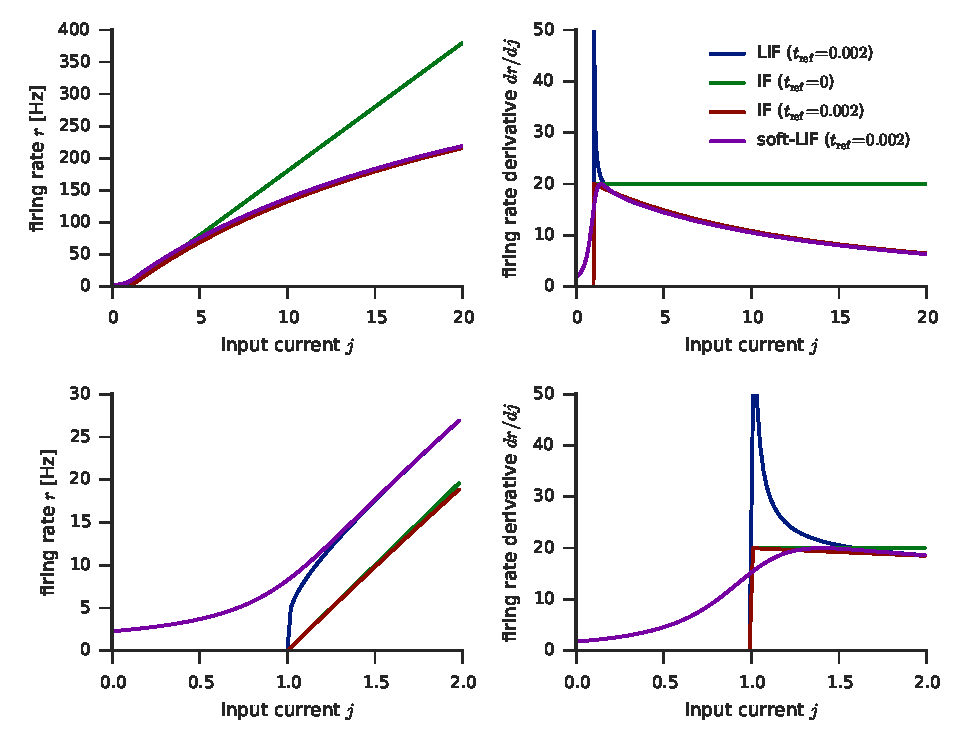
\includegraphics[width=\columnwidth]{derivative.pdf} \\
  \captionb{Comparison of neuron derivatives (right)
    and the response functions on which they are based (left).}{
    The top row shows the functions across a wide range of input currents.
    The bottom row shows their behaviour around the firing threshold.
  }
  \figlabel{learning-derivatives}
\end{figure}


\fig{learning-derivatives} shows three different neural response functions
and their corresponding derivatives.
Since the goal is to implement spiking networks in LIF neurons,
only the LIF response function is representative
of the firing behaviour of the neurons themselves,
but the singularity in the LIF response derivative around the firing threshold
prevents it from being used within a learning algorithm.
One option for a surrogate derivative function
is to simply use the LIF derivative function,
but with the value ``clipped'' to fall within a reasonable range.

The other functions shown in \fig{learning-derivatives}
can also be used as surrogate derivatives for LIF neurons.
The IF curve with no refractory period ($\tref = 0$)
is identical to the ReLU unit common in machine learning;
its derivative is simply a scaled step function.
The IF neuron with refractory period ($\tref = 0.005$)
introduces saturation in the firing rate.
Near the firing threshold, it acts linearly (as does the other IF curve),
but for larger input currents the firing rate saturates
and it approaches the LIF curve.
The derivative is qualitatively similar to that of the LIF neuron
everywhere except near the firing threshold,
where it does not suffer from the singularity present in the LIF neuron.
The equation for the IF curve is
\begin{align}
  r(j) = \left[\tref + \taurc \frac{1}{\rho(j - 1)}\right]^{-1}
\end{align}
where $\rho(x) = \max(x, 0)$ is the rectified linear function.
In contrast, the LIF curve is given by
\begin{align}
  r(j) = \left[\tref + \taurc \log\left(1 + \frac{1}{\rho(j - 1)}\right)\right]^{-1} \text{ .}
\end{align}
Since $\log(1 + x) \approx x$ for $x$ near zero,
for large values of $j$ the two curves become indistinguishable.
It is only around the firing threshold that the two functions behave differently.
The same is true of their derivatives, as shown in the figure.
Thus, the derivative of the IF curve with refractory period
is a good surrogate for the LIF derivative.

The soft-LIF neuron developed in the previous chapter
can also be used to provide a surrogate derivative for the LIF neuron.
By controlling the smoothing parameter $\gamma$,
we can control how closely the soft-LIF curve approximates the LIF curve;
larger $\gamma$ leads to a better approximation,
but also results in more extreme values in the derivative.
To facilitate comparison with the other derivative functions,
I chose $\gamma = 0.146$ such that the maximum value of the soft-LIF derivative
equaled the same maximum value as the other surrogate derivative functions.

% not addressing biological mechanisms of backpropagation
One aspect of this problem that I do not address here
are the biological mechanisms by which error or derivative information
may be transmitted within a neuron.
FA uses a three-factor learning rule,
with factors corresponding to the presynaptic neuron activity,
the derivative of the postsynaptic neuron activity,
and the projected error.
Since the postsynaptic neuron activity is based on all the incoming signals
to the postsynaptic neuron,
it is not locally available at the afferent synapses in question
without some process to transmit it back from the soma through the dendrites.
This is the function often credited to backpropagating action potentials,
which behave analogously to axonal (forward) action potentials,
but traveling backwards from the cell soma into the dendrites.
The postsynaptic neuron activity is something that is required
in many different learning rules, including all Hebbian and STDP-based rules.
To get this information to the synapses,
the backpropagating action potentials would have to be timed or transmitted
in such a way that they would not interfere with electrical currents passing
forward through the dendrites (from synapse to soma).
In this thesis, I am not modelling backpropagating action potentials explicitly,
thus I do not account for any of these potential interference effects.


\subsection{Spiking details}
\scnlabel{fa-spiking}

One of the main goals of this chapter is to implement FA
in a biologically plausible spiking network model.

% Limitations of Lillicrap spiking model
Along with the original presentation of the FA algorithm,
\textcite{Lillicrap2014} present a spiking implementation.
However, their model has a number of limitations:
\begin{enumerate}
  \item It does not use spiking neurons with a state,
    but rather uses sigmoidal neurons that spike stochastically
    with a probability given by the sigmoid function.
    This makes it significantly easier to find the neuron derivative.
  \item To represent both positive and negative feedback errors,
    the feedback path also uses neurons with a sigmoid response,
    but centred around zero and thus allowing negative firing rates.
    The authors justify this use of negative firing rates
    by referencing climbing fibres in the cerebellum,
    which fire tonically and raise or drop their firing frequency
    around this tonic rate to code positive or negative errors, respectively.
    They provide no evidence that cortical cells use such a coding scheme.
  \item The model consists of only a single hidden layer.
    This simplifies the timing problem,
    by limiting the maximum possible delay in the network.
    It also does not address issues around error transmission,
    since for one layer all FA variants (GFA, LFA, DFA) are equivalent.
\end{enumerate}

There are two subsequent papers---%
\textcite{Neftci2017} and \textcite{Samadi2017}---%
that address some of these issues in spiking neurons
(see \scn{fa-bg} for summaries).
Both use the direct variant of FA,
which is simpler to implement in spiking neurons
because it does not require mixing derivative information
into the feedback chain like GFA,
and also makes it easier to code both positive and negative errors
using nonlinear feedback neurons
due to the lower dimensionality of the error signal.

\begin{figure}
  \centering
  \tikzstyle{line} = [draw]

\begin{tabular}{c|c|c}
  BP & FA & My model \\
\begin{tikzpicture}[->,>=stealth',auto,node distance=1.2cm,
    thick,circnode/.style={circle,draw,inner sep=2}]
  \node[circnode] (h) {$h$};
  \node[circnode] (d) [right of=h, node distance=2cm] {$\delta$};
  \node[] (ah) [above of=h] {};
  \node[] (bh) [below of=h] {};
  \path[line] (bh) -- node [right] (W) {$W$} (h);
  \path[line] (h) -- (ah);
  \node[] (ad) [above of=d] {};
  \node[] (bd) [below of=d] {};
  \path[line] (ad) -- (d);
  \path[line] (d) -- node [right] {$W^T$} (bd);
  \path[line] (h) to [out=45,in=135] node {$h'$} (d);
  \path[line] (d) to (W);
\end{tikzpicture}
&
\begin{tikzpicture}[->,>=stealth',auto,node distance=1.2cm,
    thick,circnode/.style={circle,draw,inner sep=2}]
  \node[circnode] (h) {$h$};
  \node[circnode] (d) [right of=h, node distance=2cm] {$\delta$};
  \node[] (ah) [above of=h] {};
  \node[] (bh) [below of=h] {};
  \path[line] (bh) -- node [right] (W) {$W$} (h);
  \path[line] (h) -- (ah);
  \node[] (ad) [above of=d] {};
  \node[] (bd) [below of=d] {};
  \path[line] (ad) -- (d);
  \path[line] (d) -- node [right] {$B$} (bd);
  %% \path[line] (h.north) to [out=45,in=45] node {$h'$} (W);
  \path[line] (h.north) .. controls +(right:5mm) and +(up:5mm)
                        .. node {$h'$} (W.north east);
  \path[line] (d) to (W);
\end{tikzpicture}
&
\begin{tikzpicture}[->,>=stealth',auto,node distance=1.2cm,
    thick,circnode/.style={circle,draw,inner sep=2}]
  \node[circnode] (h) {$h$};
  \node[circnode] (d) [right of=h, node distance=2cm] {$e$};
  \node[] (ah) [above of=h] {};
  \node[] (bh) [below of=h] {};
  \path[line] (bh) -- node [right] (W) {$W$} (h);
  \path[line] (h) -- (ah);
  \node[] (ad) [above of=d] {};
  \node[] (bd) [below of=d] {};
  \path[line] (ad) -- (d);
  \path[line] (d) -- (bd);
  %% \path[line] (h.north east) to [out=45,in=45] node {$h'$} (W);
  \path[line] (h.north) .. controls +(right:5mm) and +(up:5mm)
                        .. node {$h'$} (W.north east);
  \path[line] (d) to node [below] {$B$} (W);
\end{tikzpicture}

\end{tabular}

  \captionb{Comparison of spiking architecture with FA and BP.}{
    The spiking architecture used here is identical to DFA,
    except that it uses an independent error population
    at each layer of the network.
    Since all the error populations encode the same output-layer error
    using population coding,
    this method is mathematically identical to DFA.
    However, it introduces a more biologically plausible delay structure
    into the network.
  }
  \figlabel{fa-spiking-arch}
\end{figure}

% Compare to Neftci methods
% - does not update in first 50 ms of digit presentation
% - update when pre-synaptic neuron spikes
The spiking network exhibited in this chapter is a type of DFA (\fig{fa-spiking-arch}).
While it shares a number of similarities with \textcite{Neftci2017},
it was developed independently \parencite{Hunsberger2017}.
There are notable differences between the two networks:
1) I use population coding to transmit the error backwards;
2) my network uses continuous learning,
whereas their network has a blackout period at the start of each stimulus presentation
when no learning occurs.

Rather than having only one error population,
I use population coding to transmit the error backwards
from each layer to the previous layer.
This is a more biologically plausible connection structure,
since it avoids many long range connections from the output layer
to each of the hidden layers.
In doing so,
it accounts for transmission delays in the feedback channel,
which biological networks have to overcome.
It also bears some similarities to LFA,
since the connections between feedback populations do appear roughly random,
though they are designed to ensure no error information is lost in the transmission.

The learning blackout period at the start of each stimulus presentation,
as employed by \textcite{Neftci2017},
ensures that no learning occurs while the network is in transition
and neuron spiking in the forward and backward pathways
is not yet reflective of the new stimulus and error.
This idea may have some biological support,
since if the error signal is internally generated (as it must be in biological systems)
then it would likely be triggered by the stimulus in some way.
Yet a biological system would not be able to turn off learning instantaneously;
there would still be residual activities in the neurons when a stimulus changes,
which may drive incorrect learning in the system for a brief time.
The network presented here uses continuous learning,
which results in slightly less efficient learning.

% How derivative is calculated
% - Right now I do ``cheat'' by using the sum of input currents. Make it so I
%   don't cheat (probably only using step function), have comparison.
% - need tolerance so that almost-zero activity is treated as zero
Both networks compute a neuron's local activity derivative
based on the current input to that neuron.
This has potential biological limitations,
since it is unclear how a specific synapse
would be able to use a derivative
that is dependent on the inputs to all synapses in the neuron.
It seems more plausible that the neuron derivative would be computed
based on the neuron output (spikes),
and the signal carried to the dendrites via backpropagating action potentials.
From a computational perspective,
this adds additional noise to the derivative signal,
and interferes with learning.
The networks presented here will use a derivative signal
computed on the total synaptic input to the cell,
as other implementations have.
Implementing a derivative based on spiking neuron output
remains an area of future work.


\subsection{Datasets}
\scnlabel{learning-datasets}

I use three different problems to evaluate the FA networks:
the \emph{linear} problem, the \emph{banded} problem, and the MNIST dataset.

In the linear problem,
the network has to learn a linear transform
from a higher-dimensional space to a lower-dimensional space.
Specifically, we have an $m \times n$ matrix of $m$ normally-distributed
$n$-dimensional input data points $\mat X$,
and our $d$-dimensional output targets are $\mat Y^* = \mat X \mat T$,
where $\mat T$ is an $n \times d$ matrix.
I orthogonalize the transform such that each dimension in the output space
corresponds to an orthogonal vector in the input space (\ie/ $T^T T = I$).
Learning is performed using a square cost (\ie/ MSE).
While this may sound like a trivial problem,
it is non-trivial for a network of non-linear neurons
to approximate a linear transform,
particularly if the neurons are nowhere linear (\eg/ LIF neurons or sigmoid neurons).%
\footnote{Since rectified linear units (ReLUs), also known as IF neurons,
  are linear above the firing threshold and silent below,
  two such neurons can perfectly fit a line (with appropriate weights).
  Therefore, networks of these neurons can solve the problem exactly.
  A network with one hidden layer would need $2d$ of these neurons
  for the exact solution.}
When training on this dataset,
I continuously generate new input-output pairs
during training using the transform.
Since no example is seen more than once,
the error during training is an unbiased measure
of the generalization (testing) error.

\begin{figure}
  \centering
  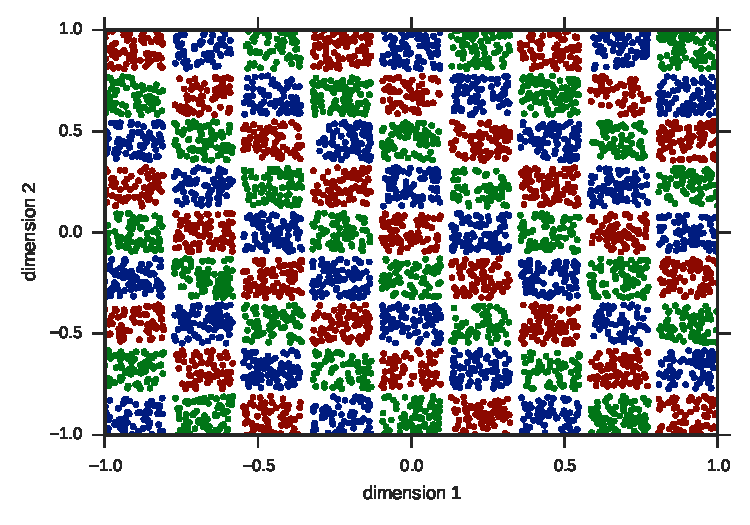
\includegraphics[width=5in]{banded2d_dataset.pdf}
  \captionb{Samples from the \dd/ banded dataset.}{
    The colours of points denote to which of the three categories they belong.
    Looking at only a single dimension gives no information
    about the class to which a point belongs
    (\ie/ the marginal distributions for all classes are identical).
  }
  \figlabel{banded-dataset}
\end{figure}

In the banded problem (\fig{banded-dataset}),
the data is arranged into bands in each dimension,
and the class of a datapoint is determined by which band it is in.
The mapping from bands to classes can be chosen such that
a single dimension contains no information about the class of a point;
only by using both dimensions can the class be determined (see \fig{banded-dataset}).
I will use this fact to help me distinguish some of the key differences
between different learning algorithms,
in terms of what kind of data distributions they are and are not suited to learn.

As a more challenging and realistic learning problem,
I use the MNIST dataset (\scn{datasets}).


\section{Results}

Since FA is still a relatively new algorithm,
there are many aspects of it that have not been well explored.
My goal with this chapter is to create a spiking model of FA learning,
in order to investigate whether the FA algorithm is a biologically plausible method
by which the brain may perform deep learning.
Before presenting the spiking model, however,
I first present some supporting results
to help justify my spiking architecture (see \scn{fa-spiking}),
including results comparing the different FA variants
and the different possible choices for the LIF neuron derivative.
I then present a fully spiking implementation
of the modified DFA algorithm (see \scn{fa-spiking})
using LIF neurons.
All rate-based experiments use the LIF rate nonlinearity
unless otherwise noted.

Throughout these results, I have made an effort to choose hyperparameters
such that BP and FA are directly comparable.
As noted in \scn{fa-parameters},
the scale of feedback weight matrices in FA can have
a very large effect on algorithm performance and learning rate,
since it can have an identical effect to setting individual learning rates
for each hidden layer.
To this end, I try to choose the overall learning rate
such that BP performs as well as possible.
Then, I choose the scale of the feedback matrices for FA
such that it performs as well as possible,
using the same overall learning rate as with BP.
This helps ensure that neither algorithm has an unfair advantage over the other
simply by having better-tuned learning rates.\footnote{
A better approach would be to use a hyperparameter optimization method
to find the ideal parameters for each algorithm,
but that is significantly more time-consuming.}


\subsection{FA variants}
\scnlabel{fa-variants-results}

I compared the performance of the different FA variants
(GFA, LFA, and DFA; see \scn{fa-variants})
on both the linear transform and MNIST learning tasks,
to look for differences between the algorithms in performance and stability.

\begin{figure}
  \centering
  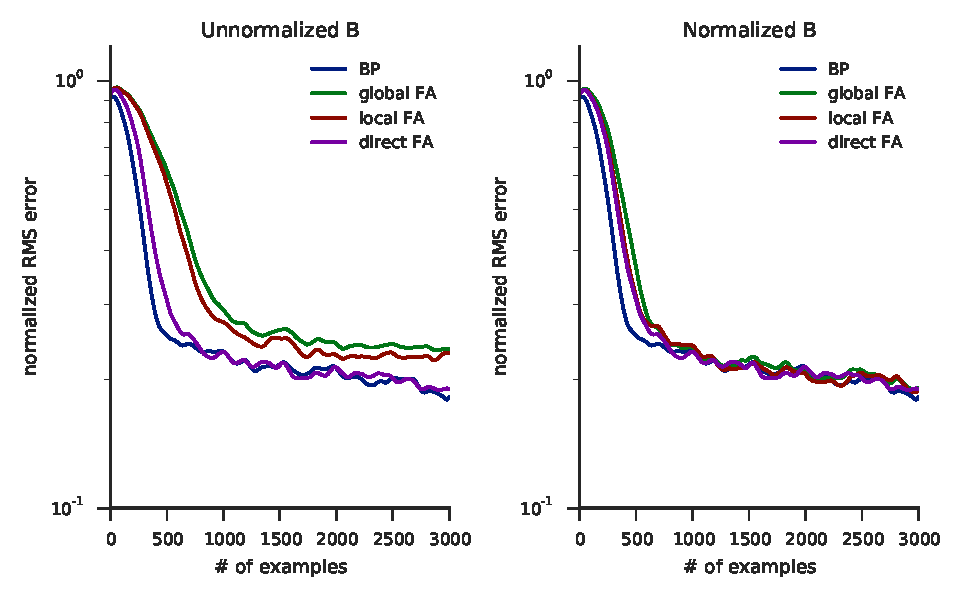
\includegraphics[width=6.35in]{variants_offline_linear.pdf}
  \captionb{Comparison of FA variants on the linear-transform problem.}{
    In the left panel,
    all feedback ($\mat B$) matrices have been generated to have the same norm (0.2).
    However, this gives larger-magnitude errors in the early layers of direct FA
    as compared to global and local FA,
    since their early-layer errors are the result
    of passing through multiple $\mat B$ matrices.
    In the right panel, the $\mat B$ matrices have been normalized so that the
    early-layer errors in GFA and LFA will have the same magnitude as with DFA.
    In this situation, we see that the variants all perform comparably.
  }
  \figlabel{variants-linear}
\end{figure}

\fig{variants-linear} shows the results on the linear transform problem.
It looks at two cases:
The first is where all $\mat B$ matrices have the same norm
across all different variants of FA.
However, since GFA and LFA both pass the output error through multiple
$\mat B$ matrices when propagating it to earlier hidden layers,
having a matrix norm less than one can mean that the magnitude of the error signal
becomes significantly smaller in earlier layers.
This can be seen in the results, where the GFA and LFA algorithms
both learn significantly slower than DFA and BP.

To account for this, I looked at a second case where
I normalized the magnitudes of the $\mat B$ matrices for the GFA and LFA algorithms,
such that the combined magnitudes of the $\mat B$ matrices
leading back to a given hidden layer
equals the magnitude of one of the $\mat B$ matrices in the DFA algorithm.
This ensures that the magnitudes of the errors at each hidden layer
are approximately the same.\footnote{
  This assumes a linear feedback path, which is the case for LFA,
  but not for GFA.
  Since GFA has the hidden unit derivatives included in the feedback path,
  the feedback error will be slightly smaller,
  since some of the hidden units at each layer are off and thus silence
  the corresponding element of the error signal.
  For this experiment, I used a step derivative function,
  and chose the feedforward amplitude on the LIF neurons
  such that the derivative equals one when the neuron is active.
  This allows GFA to be comparable to DFA and LFA,
  since the derivative does not have a scaling effect on the error,
  other than to silence some elements.}
With these normalized weights,
all the FA algorithms learn quite comparably on the linear problem,
and perform similarly to BP.
It is interesting to note that the inclusion of the neuron derivatives
in the feedback pathway does not appear to benefit GFA,
despite these same derivatives playing an important role in the BP algorithm.
This suggests that GFA is not making use of these derivatives in any
meaningful way,
due to the lack of correspondence between
the role that each neuron plays in the feedforward network computation
and randomly-projected error signal that drives the learning.


\begin{figure}
  \centering
  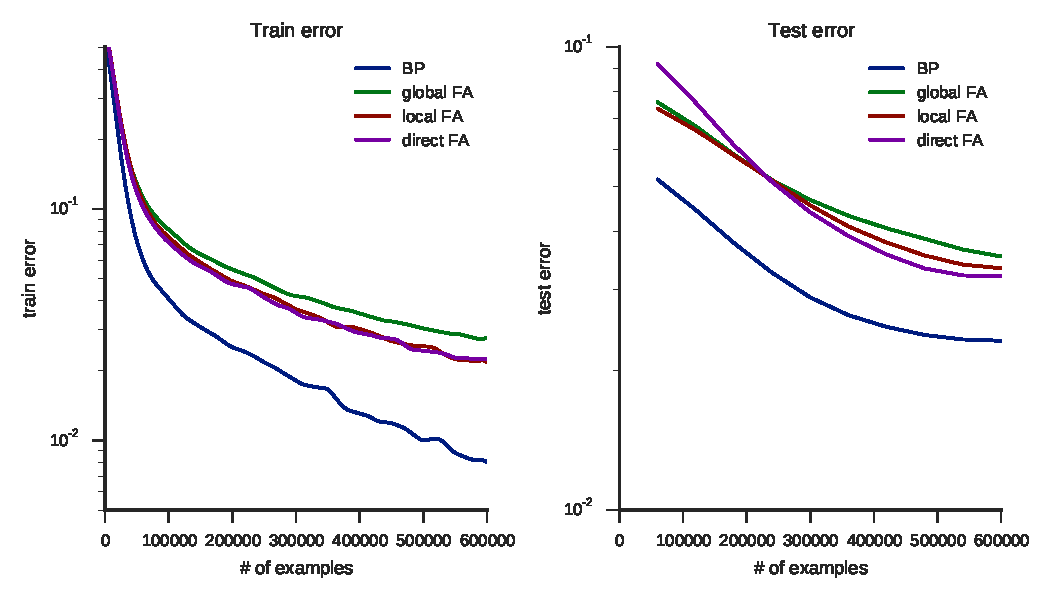
\includegraphics[width=6.35in]{variants_offline_mnist.pdf}
  \captionb{Comparison of FA variants on the MNIST dataset.}{
    The FA variants perform similarly on MNIST.
    GFA learns slightly slower,
    because the neural derivatives in the feedback pathway
    set some error components to zero
    (this experiment uses a step function as the surrogate derivative,
    scaled so that the output is unity if the neuron is active).
  }
  \figlabel{variants-mnist}
\end{figure}

To better understand whether there are performance differences
between the FA variants and BP,
I also compared them on the MNIST dataset (\fig{variants-mnist}).
This dataset is more challenging,
and shows more difference between the algorithms.
First, BP significantly outperforms all the FA variants,
scoring significantly better on both the training and test sets.
The FA results depend on the run;
a specific randomly-generated feedback matrix can be responsible
for considerable changes in performance,
particularly generalization performance.
One result that is consistent, however,
is the rate at which the training error decreases for different FA variants.
DFA and LFA both show similar rates of training error decrease,
and are faster than the decrease shown by GFA.
This is because GFA reduces the magnitude of the error signal
by multiplying by the neural derivatives
(which for this experiment are given by a step function that outputs zero or one),
while LFA and DFA do not.


\begin{figure}
  \centering
  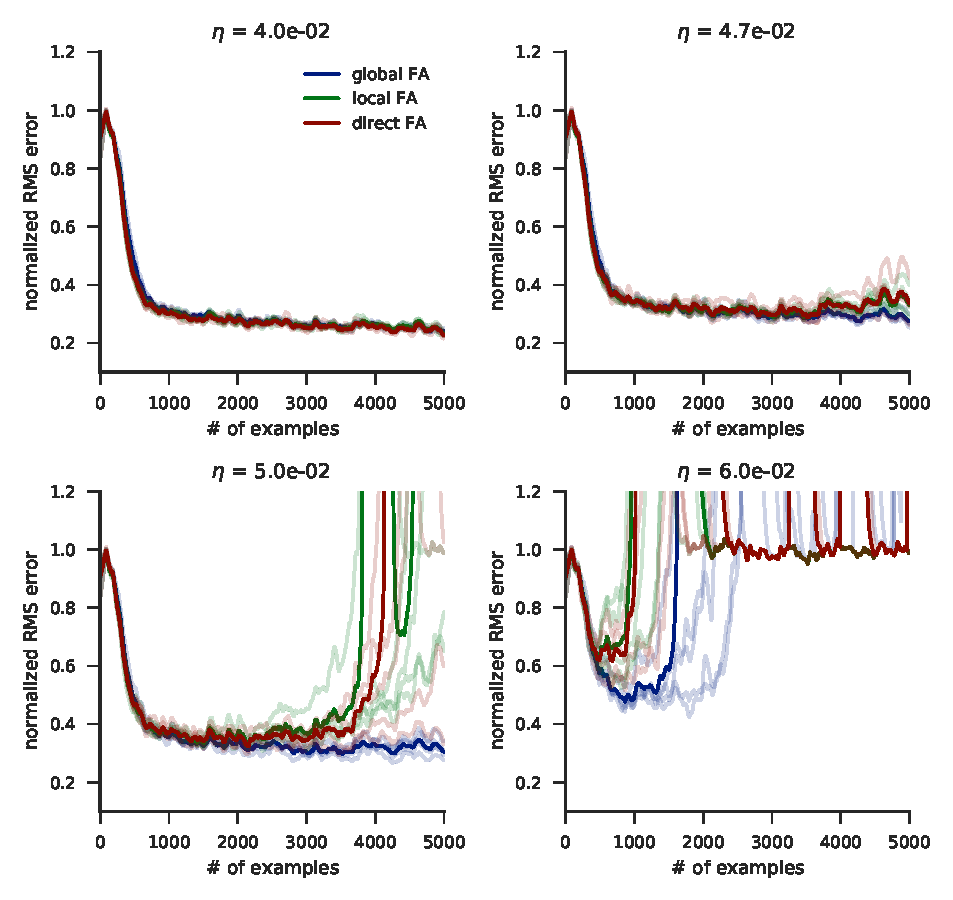
\includegraphics[width=6.35in]{variants_offline_linear_critical.pdf}
  \vspace*{-2.5em}
  \captionb{Comparison of FA variant stability on the linear-transform problem.}{
    To evaluate FA variant stability,
    this figure compares the three variants with different learning rates.
    At the lowest rate ($\eta = 0.04$), all the variants are stable.
    At the moderate rate ($\eta = 0.05$), LFA and DFA lose stability,
    but GFA is still marginally stable.
    At the highest rate ($\eta = 0.06$), all are unstable.
    What is noteworthy is that these learning rates are so close together,
    suggesting that GFA does not significantly improve stability.
    The fact that it is slightly more stable is likely simply because
    the derivative terms in the error set some values to zero,
    making the overall magnitude of the projected error smaller.
  }
  \figlabel{variants-stability}
\end{figure}

Despite being slightly slower to learn than LFA and DFA,
it is possible that GFA is more stable
because it keeps the derivative in the feedback chain.\footnote{
  I investigated a local variant of BP,
  where the derivative is not used in the feedback chain,
  and found that it is significantly less stable than ordinary BP.}
To test this, I investigated the three FA variants with learning rates
around the point at which the algorithms begin to lose stability.
I used the linear problem,
and as before, I scaled the amplitude of the LIF neurons
so that when using a step derivative,
it would output one if the neuron is active and zero if silent,
thus not scaling the error for active neurons.
As shown by \fig{variants-stability},
when the overall learning rate $\eta = 0.04$,
all three algorithms are stable.
Increasing $\eta$ to 0.05 causes LFA and DFA to lose stability, but not GFA.
Increasing $\eta$ again to 0.06 causes GFA to lose stability as well.
Thus, GFA loses stability at a slightly higher learning rate than LFA and DFA
(on the linear problem).
However, this can be explained by the fact that the error signal in GFA is
slightly smaller,
since some of the error elements are zeroed by the derivatives.
My conclusion is that GFA is not inherently more stable than LFA or DFA,
and there is no benefit to using the derivatives in the feedback pathway.


\subsection{Derivatives}
\scnlabel{fa-derivatives-results}

\begin{figure}
  \centering
  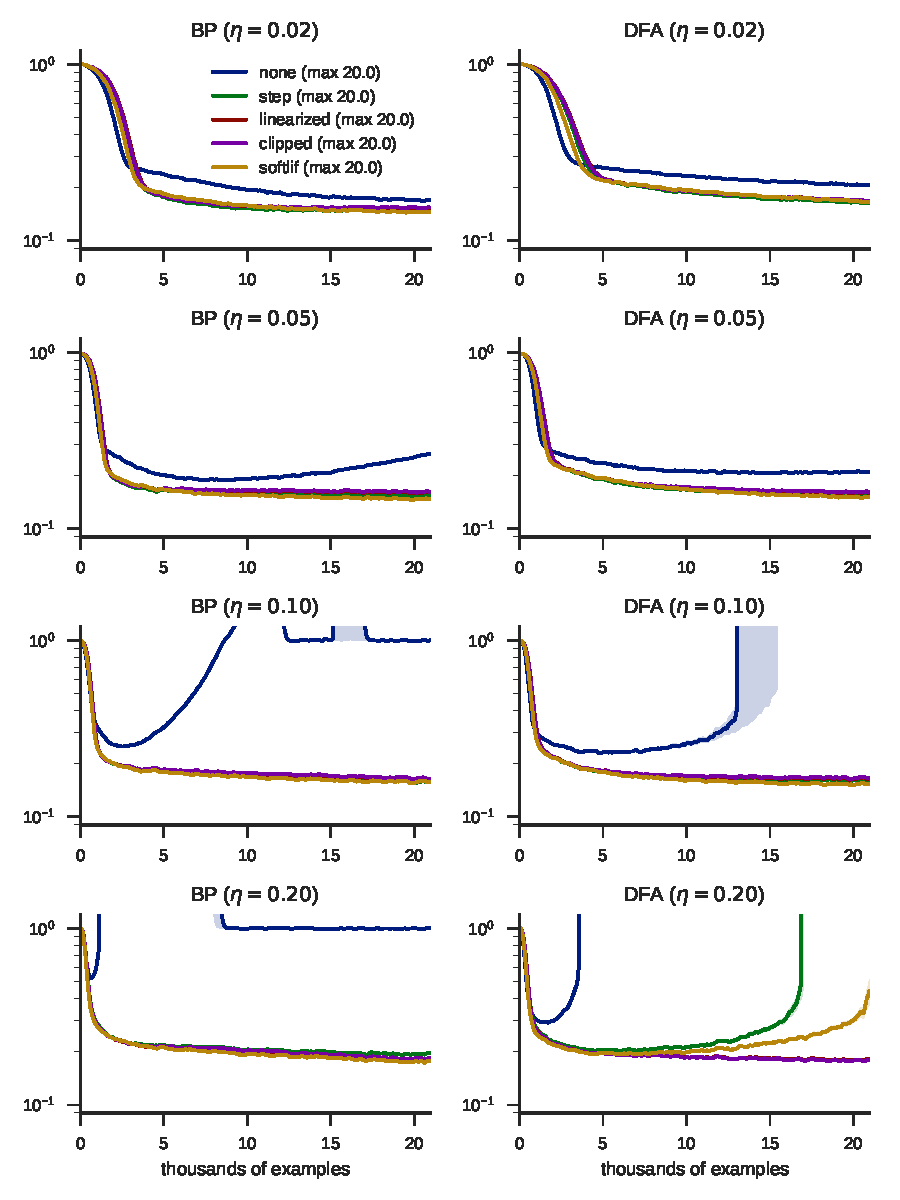
\includegraphics[height=6.4in]{derivative_offline_linear_multi.pdf}
  \captionb{Comparison of alternative neuron derivatives on the linear problem.}{
    The left column shows BP performance, the right column FA performance.
    Having no derivative (``none'') causes significant stability problems
    for both BP and DFA.
    The other derivatives perform similarly,
    except with high learning rates with DFA,
    where the step and soft-LIF derivatives lose stability
    before the clipped LIF and IF (``linearized'') derivatives.
  }
  \figlabel{derivative-offline-linear}
\end{figure}

\fig{derivative-offline-linear} compares different LIF surrogate derivatives
on the linear problem.
I normalized all derivatives to have the same maximum value,
to reduce effects due to one derivative simply having a larger magnitude than another
(see \fig{learning-derivatives} for an illustration of the derivatives).
For BP (left column), having no derivative (``none'')
leads to qualitatively different results than all of the surrogate derivatives.
Even at low learning rates ($\eta = 0.02$),
where the no derivative option appears stable,
it still learns considerably more slowly.
It becomes unstable even at moderate learning rates ($\eta = 0.05$).
The same is the case for FA, where having no derivative is unstable
at $\eta = 0.1$.

The other derivatives all appear equally stable when used with BP,
and learn equally well.
The same is true with FA across most learning rates.
At the highest learning rates, which begin to test the algorithm's stability,
the step-function derivative becomes unstable first,
followed by the soft-LIF derivative.
The clipped LIF derivative and IF derivative (``linearized'')
show the best stability and learning characteristics,
performing equally well across all the test cases.
A careful examination of the behaviour at the smallest learning rate
shows that in that case,
the soft-LIF derivative is able to learn slightly faster
than the other derivatives;
this is possibly because it is non-zero just below the firing threshold,
thus helping neurons on the verge of firing to get involved.

\begin{figure}
  \centering
  \includegraphics[width=6.35in]{{derivative_offline_mnist_multi_eta=0.020_log}.png}
  \captionb{Comparison of alternative neuron derivatives on the MNIST dataset.}{
    Again, having no derivative is problematic to learning.
    All other derivatives perform similarly with BP,
    but with FA the step derivative performs slightly worse.
  }
  \figlabel{derivative-offline-mnist}
\end{figure}

\fig{derivative-offline-mnist} shows a similar experiment using the MNIST dataset.
Again, using no derivative is clearly detrimental to learning.
More surprisingly, the step derivative function
performs as well as other derivative functions when used with BP,
but slightly worse than the others when used with FA.
Overall, FA performs worse than BP in terms of both training and testing error.


\subsection{Selectivity}
\scnlabel{fa-selectivity-results}

One of my hypotheses for how FA works
is that the random feedback weights
push neurons to be selective for different categories.
I investigated this hypothesis by looking at
the correlation between a neuron's feedback weights $\mat B^i$
and its activity in response to stimuli of each different class.
To do this, I trained a 784-500-500-10 network on MNIST.

\begin{figure}
  \centering
  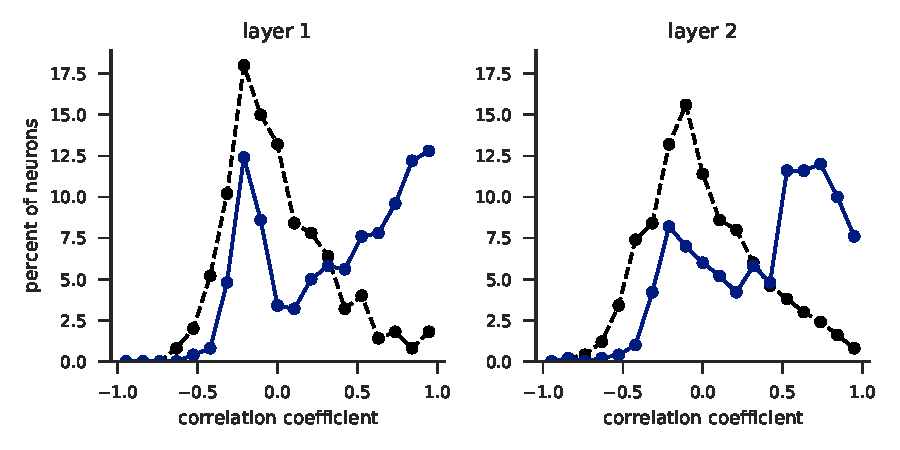
\includegraphics[width=6in]{selectivity_offline_mnist_corrhist.pdf}
  \captionb{Correlation between neural activities and feedback weights.}{
    Histograms of correlation coefficients between
    the vector of a neuron's mean activity
    across stimuli from each different class
    and its feedback vector,
    for the two hidden layers of a 784-500-500-10 MNIST network.
    Dashed lines show the initial (random) weights,
    solid lines show after training with DFA.
    The activity and feedback vector are generally positively correlated
    after training,
    indicating that DFA does push neurons to be more selective
    for particular classes over others.
  }
  \figlabel{selectivity-corr}
\end{figure}

\fig{selectivity-corr} shows the correlation between
the feedback weights for a neuron
and the pattern of activity for that neuron across classes
(in a DFA network).
The post-training histogram of correlation coefficients is skewed significantly
to the positive side for both layers,
suggesting that FA does push neurons to be selective for particular classes.
The shift from before to after training is also clearly positive.
Yet the correlation between activity and feedback vector is not perfect.
This is indicative of the fact that neuron weights are only updated
when there is an error.
So for example, if the network is able to learn to classify the digit ``1''
(one of the easier digits to distinguish)
early on in the training,
then there will be few errors on 1s,
and neurons that are mostly tuned to that digit
will have fewer changes in weights.
Also, some neurons may be ``naturally'' tuned (based on their initial feedforward weights)
to a set of digits completely different than what their feedback weights
are pushing them towards.
Such neurons may end up with activities that are more correlated
with their feedback weights,
but may never become strongly correlated.


\subsection{Limitations}
\scnlabel{fa-limitations-results}

As described previously (\scn{fa-intuitions}),
one intuition for what FA is doing
is that the feedback weights are pushing the hidden neurons
to each be selective to different output classes,
thus making them useful for decoding class information.
This has an apparent limitation:
if hidden neurons in a particular layer
do not have the information that they need
to be selective for one class over another,
then pushing them to be selective for some classes
is simply going to push them in random directions.
To both illustrate and demonstrate this limitation,
I have designed a network where this is the case.
For this, I use the \dd/ banded dataset (see \scn{learning-datasets}),
which has the property that class information can only be determined
using both input dimensions.\footnote{
  Put another way, the marginal distributions across either input dimension
  contain no class information.}
Using this dataset, and limiting each first-layer neuron to only receive input
from one input dimension or the other,
results in a problem that BP is able to solve but FA is not.
For simplicity, this experiment uses ReLU neurons.

\begin{figure}
  \centering
  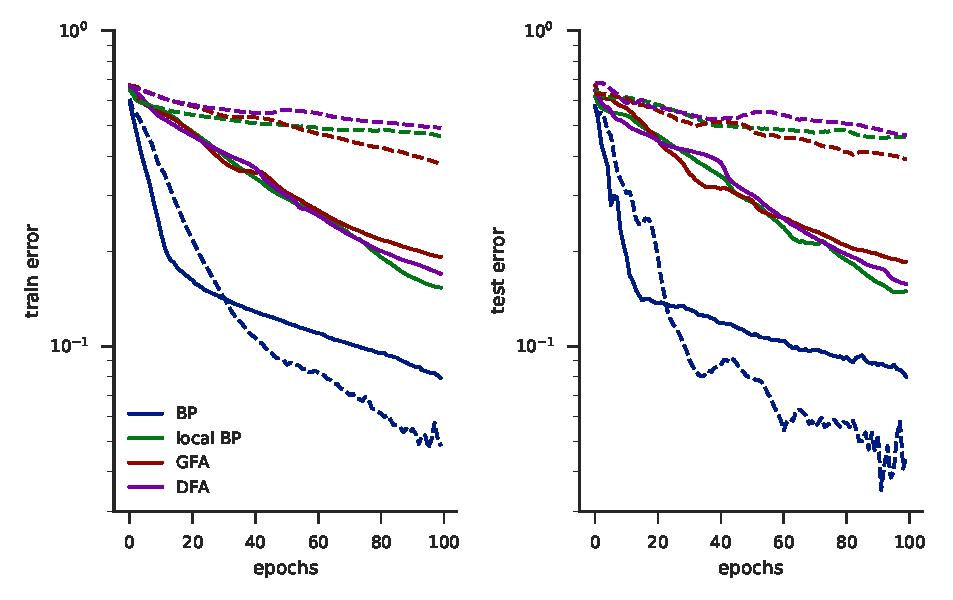
\includegraphics[width=6.35in]{banded2d_losses.pdf}
  \captionb{Comparison of learning methods on the \dd/ banded dataset.}{
    The solid lines show the fully-connected case,
    where first-layer hidden neurons are connected to both input dimensions.
    The dashed lines show the limited-connectivity case,
    where each first-layer hidden neuron connects to
    only one of the two input dimensions or the other.
    Learning is impaired in the limited-connectivity case for
    GFA, DFA, and local BP, but not for standard BP.
  }
  \figlabel{banded2d-comparison}
\end{figure}

The upper panel of \fig{banded2d-comparison}
shows the experiment where the input (first-layer) weights are unconstrained;
that is, first-layer hidden neurons can receive input from both input dimensions.
In this case, both BP and FA are able to learn.
BP still outperforms FA on the task, though;
this is because the number of neurons in the first layer
is too low for FA to have one neuron per section on the grid.
In the constrained case,
where each first-layer neuron only receives input
from one of the two input dimensions,
we see that FA performs much worse.
This suggests that FA is unable to properly solve the credit assignment problem
to learn hierarchically.
BP, on the other hand, \emph{is} able to learn hierarchically,
and performs better.

% Fact that local BP also does poorly reflects importance of
% derivative in feedback chain
It is surprising that local BP---%
that is, BP with the neuron derivatives only applied locally,
but not included in the feedback pathway---%
is also not able to solve the problem.
This suggests that the neuron derivatives are an important part
of the credit assignment process,
and not including them in the feedback pathway is detrimental.
Unfortunately, there is no obvious way to include the neuron derivatives
in FA in a useful manner.
As seen previously, and as evidenced by the poor performance of GFA on this task,
simply including the neuron derivatives in the feedback pathway (in a similar manner to BP)
is not helpful.


\subsection{Adaptive variants}

\begin{figure}
  \centering
  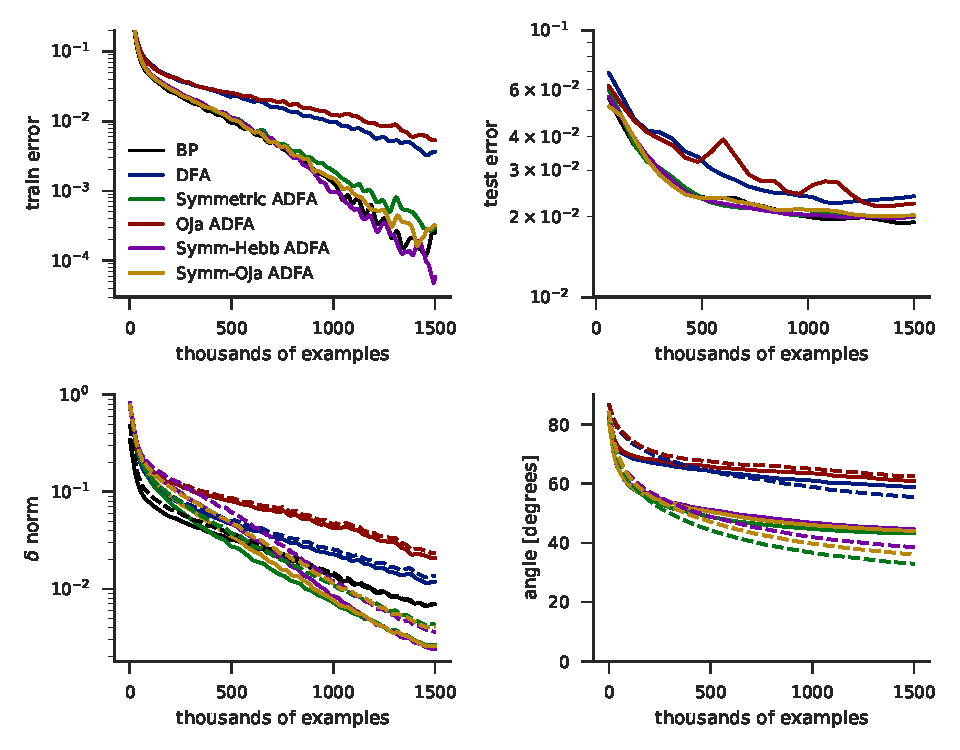
\includegraphics[width=6.35in]{adaptive_offline_mnist.pdf}
  \captionb{Comparison of adaptive variants on MNIST task.}{
    The top-left and top-right panels show the training error and testing error, respectively.
    The ability to decrease training error
    is the best reflection of each algorithm's performance.
    The bottom-left panel shows the magnitude of $\delta$,
    where $\delta$ is the projected error times the local neuron derivative.
    The bottom-right panel shows the angle between the actual (FA) update
    and the ideal (BP) update.
    In the bottom plots, solid lines show the first hidden layer,
    and dashed lines show the second hidden layer.
    For all variants, $\mu = 1.0$ and $\nu = 0.1$;
    thus the symmetric component of the adaptation
    has the same learning rate as the forward weights,
    whereas the unsupervised component (Hebbian or Oja) has one-tenth the learning rate.
    This is required for stability.
  }
  \figlabel{adaptive}
\end{figure}

I compared the performance of adaptive variants of DFA (the ADFA variants)
on the MNIST task.
Preliminary experiments indicated that the Hebbian and Oja variants
offered a performance improvement over non-adaptive DFA.
A closer examination of this result
revealed that the magnitude of the feedback weights
was smaller than optimal,
and that the benefit from these adaptive variants
was because they increased the magnitude of these weights,
thus speeding up convergence.

\fig{adaptive} shows the revised experiment
with closer to optimal feedback weight magnitude.
In this case, the Oja variant no longer performs better than DFA;
in fact, it performs slightly worse.
As in the preliminary experiments,
the Oja variant increases the $\delta$ magnitudes (and thus the learning rate),
but in this situation,
the original (unadapted) $\delta$ magnitudes were near-optimal,
and increasing them is only detrimental.
Additionally, the angles between the Oja ADFA updates
and the ideal BP updates are worse than for DFA,
thus the adaptation is not pushing the weights in a useful direction.
The Hebbian variant is not shown,
because it becomes unstable in this experiment,
even though its learning rate is one-tenth the forward learning rate ($\nu = 0.1$).

Symmetric ADFA does considerably better than DFA,
with performance nearing that of BP.
The angle between the symmetric ADFA updates and BP
is much better than the DFA angles,
since the updates are pushing both the forward and backwards weights
in the same direction, aligning them.
The combined Symmetric-Hebbian and Symmetric-Oja variants
also perform well.
Near the end of training,
their performance appears to surpass that of Symmetric ADFA,
though it is unlikely that this result is significant.


\subsection{Spiking network}
\scnlabel{fa-spiking-results}

\begin{figure}
  \centering
  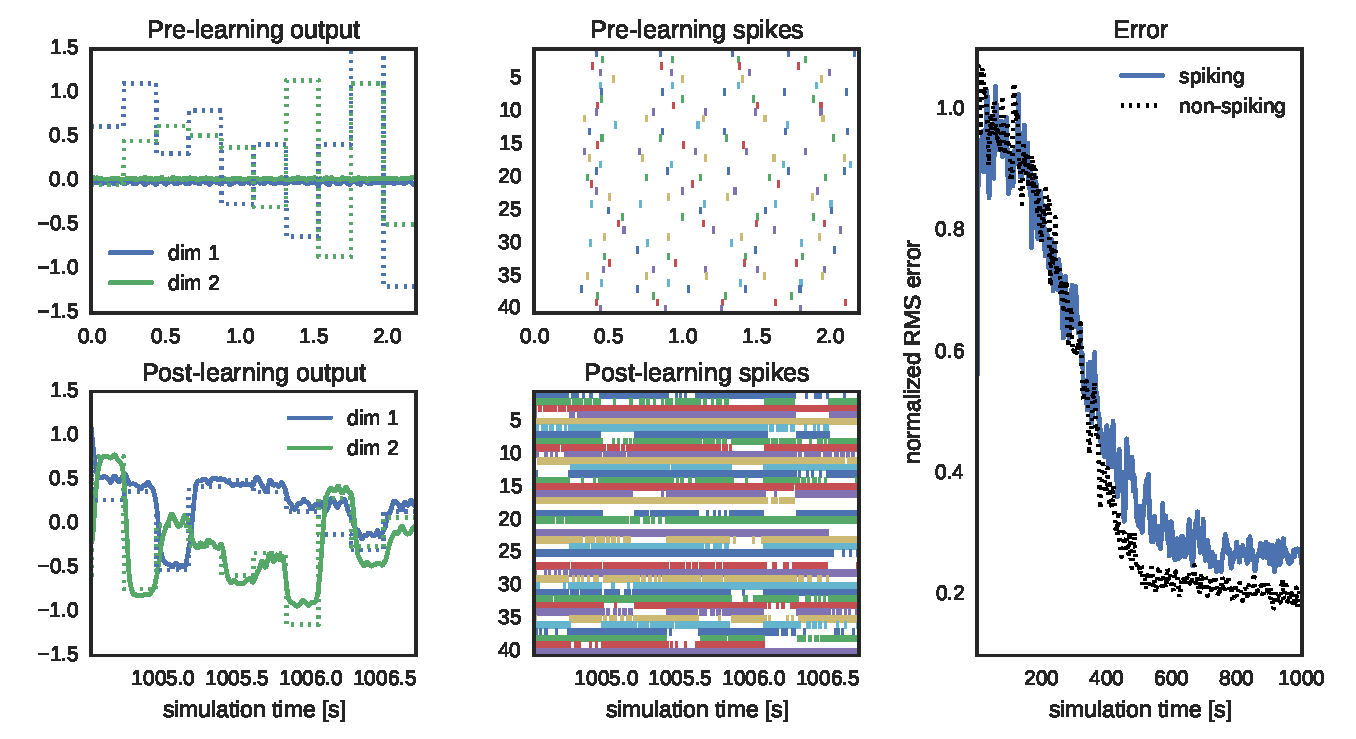
\includegraphics[width=\columnwidth]{../cosyne_poster/figures/online.pdf}
  \captionb{Spiking network learning the linear problem.}{
    The left panels show the network output (solid traces)
    as compared with the desired output (dotted traces)
    before and after learning.
    The centre panels shows the spiking of the first hidden layer
    before and after training.
    The right panel shows the overall error rate of the spiking and rate
    networks during the course of training.
  }
  \figlabel{online-overview}
\end{figure}

A summary of the online spiking learning system is shown in \fig{online-overview}.
The system learns to perform the linear task.
The top panels show the performance of the network before learning;
there is a minimal, uniform response to all stimuli,
and the neuron spiking is sparse and does not seem to be indicative
of what stimulus is present.
The bottom panels show the performance after learning, on novel test stimuli.
The network output matches the target output values well,
and the neurons are both more active,
and appear to be selective to specific regions of the input space.
As shown by the far-right panel,
the error of the spiking network
decreases to almost the same level as that of the network trained offline.

% important factors when training spiking networks
% - presentation time for each example
% - total training time
% - learning rate
% need to balance number of examples seen (shorter pt -> better) with
% sufficient time on each example for the network to settle and learn.
% Also a tradeoff between faster learning on each example (longer pt, larger lr)
% and good learning for generalization \ie/ not overfitting/forgetting (shorter pt, smaller lr)
% Presentation time also related to learning rate,
% since larger LR will mean more forgetting of past stimuli, need quicker succession of stimuli
When learning in online spiking networks,
there are a number of different factors that affect
how well the network learns.
As with non-spiking networks,
the learning rate has a strong effect on how well the network learns.
While larger learning rates theoretically
allow the error to decrease more quickly,
if the learning rate is too large,
then the network will fit itself too much to each new stimulus,
and lose some of the information learned from previous stimuli.
This problem is more acute in online learning,
since each stimulus is shown for multiple time steps,
giving the network more time to overfit to the new stimulus.
I found that if the system is able to reduce the error to close to zero
on each new stimulus presentation, particularly during early learning,
this indicates the learning rate is too large.
Optimal learning rates showed only a slight decrease in error
over the course of each stimulus presentation,
but after many such presentations,
the network was able to learn the desired function quite well.

The presentation time for each stimulus also has a large effect on learning.
Assuming the total training time is fixed,
there is a tradeoff between showing each stimulus for a long time
and showing many stimuli.
Each stimulus must be shown for an adequate length of time to learn well,
since at the onset of each new stimulus there are considerable transients
due to past information stored in synapses and membrane voltages.
It is only once the network has settled into its feedforward state
that useful learning can occur.
However, if stimuli are shown for too long,
this decreases the number of different stimuli that can be shown
in the allotted time,
limiting the diversity that the network is exposed to and
thus reducing its generalization performance.

Finally, the total training time affects performance.
While the basic relationship is that longer training times
mean exposure to more stimuli for longer times and thus better performance,
the outcome does depend on the learning rate and presentation time.
For example, if the presentation time is long or the learning rate is high,
then increasing the total training time may not improve performance
beyond a certain point.
In this situation, the network is constantly re-fitting itself
to the most recent stimuli and forgetting the old stimuli,
so increasing the total training time will only
increase the list of forgotten stimuli.


\section{Discussion}

% FA is not perfect at doing credit assignment; some problems it can't solve.
%   Is this a showstopper, though? How much credit assignment is needed in the brain?
%   Earlier visual areas are likely trained with other objective functions,
%   not just classification as currently happens.
% - Need for synchronization between forward and backward passes might also
%   limit the maximum depth for single-objective-function learning in the brain.
One limitation of Feedback Alignment (FA)---%
and a key difference with backpropagation (BP)---%
is that FA does not truly solve the spatial credit assignment problem.
Theoretically, this is most apparent in the case of direct FA,
where all hidden neurons only receive error information from the output layer.
Since they do not receive error information from any downstream neurons (\cf/ BP),
there is no way that they can update to reduce downstream errors,
they can only try to reduce the output error directly.
Since global FA and local FA essentially reduce to direct FA\footnote{
  Local FA is mathematically equivalent to direct FA,
  and global FA is the same as local FA
  but with an essentially random perturbation (the derivative scaling)
  on the feedback errors. See \scn{fa-variants}.},
they also face the same problem.
I confirmed this empirically with the experiments in \scn{fa-limitations-results}:
In the case of the \dd/ banded problem,
where no class information is available to the first layer neuron
it is impossible for FA to learn.
FA relies on pushing all hidden neurons to be selective
for some classes over others,
rather than reducing downstream hidden-neuron errors as BP does.
The result is that there are certain problems that are unlearnable by FA.

To determine whether this limitation of FA is a serious problem,
the next question should be: ``How much credit assignment is required in a brain?''
In the human visual system,
it is quite unlikely that classification error
is the only error signal available to the system.
Not only do earlier visual layers likely learn at least partly
based on features more associated with the dorsal stream (such as depth and motion),
but there is likely unsupervised learning happening at many layers.
Therefore, the amount of supervised deep learning that occurs in the brain
is almost certainly not as all-inclusive as is the case
in the models presented here.
Thus, the fact that FA can only learn when class information is available
may not be a serious limitation:
early visual layers---where there is typically less class information---%
could learn predominantly based on other signals,
with FA taking a leading role at the higher layers of the ventral stream
where more class-specific inputs are readily available.

%%  LocalWords:  Marblestone bp biomechanisms bg dtp Bengio nef Baldi
%%  LocalWords:  Grossberg Guergiuev Bogacz Balduzzi Lillicrap
%%  LocalWords:  Liao Ioffe Nokland DFA IFA ARBP ASRBP Neftci Samadi
%%  LocalWords:  ep Scellier RBP ij GFA qj LFA lj li mnist multi DNNs
%%  LocalWords:  unlearnable backprop ADFA Symm Hebb softlif
%%  LocalWords:  unadapted

\chapter{Conclusion}
\chplabel{conclusion}

I have described three different methods
for constructing spiking neural networks:
fixed-encoding methods, spiking deep neural networks trained with backpropagation,
and spiking deep neural networks trained with Feedback Alignment.
While the ultimate goal of all the methods
is to provide insight into how the brain may solve
the object classification problem,
each method has its own unique benefits and limitations.
This chapter outlines the key contributions of this thesis
towards each of these three methods,
as well as future work to be done both for the specific methods
and to understand human object recognition as a whole.


\section{Summary of contributions}

\subsection{Fixed-encoding networks}

The first portion of this thesis
looks at spiking object classification in fixed-encoding networks.

% Comparison of Gabor filter encoders with others
This thesis proposes Gabor filters for fixed-encoding networks,
demonstrating that a randomly generated basis of Gabor filters
is a good encoding method for classifying MNIST images.
They outperform the randomly generated weights
typically used in fixed-encoding networks,
as well as the Computed Input Weights and Constrained Difference weights
approaches of data-driven encoder generation.
This suggests that Gabor filters are a better basis for classification,
despite being tuned to general image statistics,
rather than the particular statistics of the MNIST dataset.

% Characterization of the benefits of alternative loss functions for decoders
I also characterize the benefits of alternative loss functions
for solving for decoding weights in fixed-encoding networks.
Alternative loss functions have not been well explored
in these types of networks,
with almost all works relying on squared loss.
Squared loss works well for regression problems (such as those typically addressed by the NEF),
but the results of \chp{nef} show that alternative loss functions
(weighted squared loss, softmax loss, hinge loss)
result in better performance on classification problems.
While the weighted squared loss was previously introduced by \textcite{Toh2008},
it has not caught on in the ELM community,
who are the main group using fixed-encoding networks for classification.
My results underscore the need for alternatives to squared loss.

I run these fixed-encoding networks in spiking neurons,
a step that is common in the NEF paradigm
but that is not typically taken for object classification problems
(which have largely been ignored by the NEF).
The spiking networks perform almost as well their non-spiking counterparts,
indicating that this conversion is possible,
and allowing basic object classification components
to be seamlessly integrated into NEF models.
I also demonstrate that regularization is required for spiking networks
when using squared loss,
but is less essential with other loss functions,
particularly softmax loss.


\subsection{Spiking deep networks}

The middle portion of this thesis examines methods
to train spiking deep networks on more difficult object classification tasks,
including the ImageNet dataset.

% soft-LIF model
The soft-LIF model---%
a differentiable version of the LIF rate response curve---%
is a novel way to train deep spiking networks with LIF neurons.
It is both simple and efficient,
allowing it to train the first deep spiking models
on the ImageNet dataset \parencite{Hunsberger2016}.
The idea behind it---%
smoothing out the discontinuity of a neural model around the firing threshold---%
is generalizable to other neural models,
allowing deep networks to be trained with any neural model
with a fixed rate response function.

% Training with noise, and noise models
I also introduce a novel approach to account for the variation
caused by spiking neurons,
by modelling this variation and training with
stochastic variation (noise) with a similar distribution.
The results show that training with noise (in the right amount) is beneficial,
particularly when using no synaptic filters and shorter classification times.
Doing so can improve the efficiency of spiking neural networks
on neuromorphic hardware
while maintaining similar levels of accuracy (\scn{spike-efficiency}).
The method of characterizing spiking variation is also potentially applicable
to other spiking networks,
for example those developed using the NEF.


\subsection{Biological learning}

The final portion of this thesis
brings biological plausibility
into the training of deep spiking networks,
specifically via the Feedback Alignment (FA) algorithm.

% a better understanding of what FA is doing
The first contribution of this thesis in this area
is to provide a better understanding of how FA works.
I examine a number of different variants of FA (GFA, LFA, and DFA),
and find that they are all essentially doing the same thing.
Including the gradient in the feedback pathway (as with GFA)
does not contribute to the stability of the algorithm.
FA also works with a number of different surrogate gradients for LIF neurons;
it does not require the exact derivative of the nonlinearity to function.
I introduce the derivative of an IF neuron with refractory period
as a surrogate for the LIF derivative,
and find that it works better than a step derivative function
when used with FA.
I also investigate the hypothesis that FA pushes neurons
to be selective for particular classes.
I find that there is correlation between a neuron's activity
and its feedback weights in DFA,
indicating that this hypothesis is correct.
Yet the correlation is not perfect,
suggesting that there are numerous factors at play,
including the initial weights and which classes are more difficult to classify.

% some limitations of FA
Most works to date have focused on situations where FA performs similarly to BP;
\scn{fa-limitations-results} begins to identify some of the limitations of FA.
The results show that there are problems that BP can solve that FA cannot.
This indicates that FA does not fully solve the credit assignment problem.
%% This is partly due to the fact that FA requires class information
%% to be available
Interestingly, local BP (\ie/ BP without neuron derivatives in the feedback pathway)
is also not able to solve this problem.
This indicates that the inability of FA
to include derivatives in the feedback pathway in a meaningful way
contributes to its inability to fully solve credit assignment.

% Further exploration of adaptive FA
%% I further explore adaptive FA,
%% and find that Hebbian and Oja adaptive FA
%% can contribute to convergence if the feedback weights are too small,
%% but not if they are properly adjusted.
%% Symmetric adaptive FA is more beneficial,
%% since the updates are identical to those for the feedforward weights
%% and thus push the feedforward and feedback weights to align.
%% This alignment leads to convergence rates on MNIST near that of BP.

% novel spiking implementation of FA
\scn{fa-spiking-results} presents a novel spiking implementation of FA.
This spiking implementation addresses most of the problems
with BP outlined in \scn{bp-problems},
most notably some that have not been addressed by
past spiking implementations.
It uses population coding to transmit the feedback error
using nonlinear neurons, addressing the linear feedback problem.
It demonstrates that the timing problem does not prohibit learning
as long as stimuli are shown for a sufficient length of time.
It uses surrogate derivatives to allow the use spiking LIF neurons,
improving on past models by using a more biologically-plausible neuron model,
and demonstrating that surrogate derivatives can be used
without a significant effect on performance.


\section{Future work}

This section outlines some avenues of future work
that follow either directly from the work in one of the chapters,
or more generally in order for neural models of object recognition
to continue to become more biologically plausible and powerful (\scn{future-beyond}).


\subsection{Fixed-encoding networks}

% online implementations of loss functions
The weighted squared loss, softmax loss, and hinge loss examined in \chp{nef}
all showed an improvement over squared loss for classification.
It remains unclear how neurons may implement such loss functions online.
Weighted squared loss is likely the easiest to implement,
since it still has a linear derivative.
All that would be required is weighting the errors on the decoder learning
based on the correct label of the current input.
To implement softmax loss or hinge loss,
neural mechanisms would be required
for computing the nonlinear functions in their derivatives.
Expanding these loss functions for online learning in neurons
would have applications beyond fixed-encoding methods,
to any online classification learning in neurons,
including the biological learning methods examined in \chp{learning}.

For fixed-encoding methods to be truly successful,
they need to have success on more challenging datasets.
To date, their main successes are on MNIST,
with some success on CIFAR-10 \parencite{McDonnell2015a}.
A likely criterion for this success is the extension to multilayer networks,
with two or more hidden layers.
This will require better techniques for constructing features
beyond the first layer.
The nature of deep features both in the brain and in ANNs
are still poorly understood,
which makes it difficult to manually construct these features
for fixed-encoding networks.


\subsection{Spiking deep networks}
% --- spiking ANNs

% Application to state-of-the-art network models
Spiking ANNs can achieve similar performance to similar non-spiking ANNs---%
even on challenging datasets like ImageNet---as shown in \chp{spike}.
It has yet to be shown that spiking networks can match state-of-the-art
performance on these datasets.
The network on which I based my work in \chp{spike} \parencite{Krizhevsky2012}
was close to the state-of-the-art when I began,
but advances in recent years have far surpassed it.
Achieving state-of-the-art results in spiking networks using my methods
may be as straightforward as integrating them into the training procedure.
The simplicity of some modern networks
like the all-convolutional network of \textcite{Springenberg2015}
could facilitate easy integration.

% Lower firing rates in spiking networks
Both the networks introduced in \chp{spike}
and others that perform well on datasets like MNIST \parencite[\eg/][]{Diehl2015}
have spike rates (80-180 Hz) considerably higher
than those observed in cortical neurons ($\sim$10 Hz).
Lowering firing rates would both increase the biological plausibility
of the networks,
and increase the potential benefits from implementing them on neuromorphic hardware,
where energy use is often tied directly to neuron firing rates.
Recent work by \textcite{Zambrano2017} moves in this direction,
introducing networks with significantly lower firing rates
($~\sim$10 Hz on many datasets).
Yet, their networks actually require more spikes to classify each image,
due to larger network sizes (see \tab{spike-sota-rates}).
Future work is required to determine
whether the number of spikes per can be reduced,
while maintaining high levels of accuracy.

% Implementation on neuromorphic hardware
As of yet, my networks have not been tested on neuromorphic hardware.
While this is theoretically straightforward,
there are a number of technical hurdles to overcome,
particularly when targeting analog neuromorphic hardware
due to the variation between chips.
These include developing detailed models of all the neurons on the hardware,
then training the network for the specific chip in question.

On some types of neuromorphic hardware,
it is not possible to construct a static rate-response function
for the neurons,
if they include more complex dynamics such as adaptation.
For this hardware, an approach that takes neuron dynamics into account
might be required.
As of yet, most methods for training spiking neural networks---%
whether rate-based or spike-based---%
are not able to account for such dynamics.


\subsection{Biological learning}
% --- biological learning
% Better understanding of where feedback alignment fails.
% - are true Credit assignment methods required?
The results in \scn{fa-limitations-results}
outline some of the limitations of FA as compared with BP,
including the fact that FA does not truly solve the credit assignment problem.
In that case, the limitations are only apparent on a constructed problem;
it remains to be seen whether FA is limited on real-world problems,
as compared with BP.
So far, results from FA have been comparable with those of BP
for fully connected networks on the MNIST dataset.
\textcite{Nokland2016} applied FA to a convolutional network
on the CIFAR-10 dataset,
and found that it performed significantly worse than BP (see \scn{fa-bg} for details).
Part of the problem may be that convolutional networks use tied weights,
which results in many fewer parameters and thus make it more difficult
for the random feedback basis employed by FA
to function efficiently.\footnote{
  A similar effect is seen with fixed-encoding networks.
  They function almost as well as BP when using a large basis of random input weights
  to cover the entire space of inputs,
  but perform comparatively worse with only a small random basis.
  The curse of dimensionality means that as the input dimensionality increases,
  it becomes harder to tile the space with a random basis.}
  %% This is related to the fact that a large number
  %% of uniformly distributed random points
  %% will cover a high-dimensional space almost as well
  %% as if the points were uniformly tiled throughout the space,
  %% but a few random points will do a comparatively worse job covering the space
  %% as compared with the same points uniformly tiled.}
Convolutional weights are also not biologically plausible,
since the weights across different locations are exactly equal (tied),
but they do make training deep networks more efficient due to fewer parameters.
Future work should investigate whether FA is comparable to BP in a deep network
without tied weights but with limited receptive fields (\ie/ locally connected layers),
since these are most similar to the structure of visual cortex.
If FA is able to achieve similar results to BP
on more challenging datasets with such architectures,
this may be evidence that FA is sufficient
for the supervised learning problems faced by the brain.
Otherwise, a learning method that fully solves the credit-assignment problem
may be required.
Adaptive FA is one such potential algorithm.
By pushing the backwards weights to further align with the forward weights,
not only could adaptive FA reduce the error due to misaligned feedback,
but it could also allow FA to integrate neuron derivatives into the feedback pathway
in a way that they contribute to credit assignment.
Research is needed to test this hypothesis,
as well as to identify adaptation methods for FA
that are both effective and biologically plausible.

% More realistic modelling of backpropagating action potentials
% - other mechanisms involved in learning
So far, FA has mainly been investigated at a network level,
with less consideration to how individual neurons may implement
the required learning mechanisms.
\textcite{Guergiuev2017} is one exception;
their work begins to address how feedforward and feedback signals
may be managed within a single cell.
Future work is needed to expand on these networks,
for example by bringing in spiking dynamics.

% Combining FA and NEF methods


\subsection{Beyond}
\scnlabel{future-beyond}
% --- larger extensions

There are a number of open questions that go beyond the methods examined in this thesis.

% Dale's principle
While this work makes a step in the direction of biological plausibility,
there are still numerous characteristics of biological networks
that are not accounted for by any object recognition models.
One such characteristic is Dale's principle,
which for our purposes can be simplified to the rule
that neurons are either excitatory or inhibitory (in their output),
not both.
In typical ANNs, including all the networks developed in this thesis,
neurons are allowed to have both positive and negative connection weights
on their outputs.
Respecting Dale's principle would require restricting these to be
either all-positive or all-negative for each neuron,
which could have significant effects on learning.
Excitatory and inhibitory neurotransmitters also have different synaptic dynamics,
and excitatory and inhibitory neurons have different connectivity structures;
a more extensive implementation of Dale's principle
would also account for these additional characteristics.

% Localization of objects
% Need for video? attention? neuromorphic methods will excel more
% foveas?
All the methods presented in this thesis process static images,
one-at-a-time, and view each image in its entirety.
This is the way object recognition systems
have traditionally been designed and developed,
and it is still common today.
Recently, some researchers have begun focusing on object localization,
where objects are both identified (recognized)
and their position in the image is determined;
this task is included as part of the new ImageNet challenges (ILSVRC).
This allows images with multiple objects
to be processed in a more natural manner.
%% This idea of object localization also connects to attention

A next step is to begin to run object recognition networks on video,
and as part of this process,
incorporate other aspects of vision such as tracking.
%% Not only can this potentially impro
I believe that it is in such systems,
where there is a temporal aspect to the input,
that neuromorphic hardware will really offer an advantage.
No longer will the temporal aspect of spiking neurons
be holding back the efficiency of the system,
as occurs when a spiking network needs
multiple timesteps to process a static image
(whereas an ANN can process it in one forwards pass).
With dynamic inputs, spiking networks will be continuously processing,
which could allow for both efficient computation and short response times.
Traditional methods like ANNs require a new,
independent pass through the network for each video frame,
potentially making them less efficient by comparison.

% Role of unsupervised learning in visual system development
% - need to use less labelled data, do more with what we have
% - what does this suggest about NEF encoders? Encoder-selection methods
%   like a form of unsupervised learning
All methods that currently excel at object recognition---%
including all the methods in this thesis---%
rely heavily on supervised learning.
They require large sets of labeled data,
and while images are cheap, the corresponding labels are expensive,
because they require a human to provide them.
Not only is this detrimental from an engineering perspective,
it also limits the biological plausibility of the models.
Young humans learn to recognize objects using only limited labels.
A child needs only to be told a few times that a particular type of animal
is a dog or a cat,
and can quickly begin generalizing to other objects of the same class.\footnote{
  ANNs, by contrast, require thousands of labelled examples of each class.}
%% (sometimes over-generalizing, and calling all animals ``puppy'' for example).
This points to large amounts of unsupervised learning happening in the brain,
specifically a type of clustering that allows us to group objects
even when we do not have a label to apply to the group.

Accounting for such unsupervised learning will
significantly change the way we model object recognition.
For the fixed-encoding methods of \chp{nef},
ideas and methods from unsupervised learning
can inform the way we choose encoders,
so that they will better capture and separate the data.
When learning deep networks with backpropagation (\chp{spike}),
methods that combine unsupervised and supervised learning
will ideally be able to learn better generalization,
since they can take advantage of the large number of unsupervised images available.
Finally, unsupervised learning will have a dramatic effect
on the biological learning models discussed in \chp{learning}.
It will take a lot of the onus off the supervised learning method (\eg/ Feedback Alignment),
allowing the supervised methods to focus on learning the last few layers of the network,
while the unsupervised methods take care of much of the earlier learning.
This means that it is not as important if these supervised methods
can learn very deep networks,
and may mean that algorithms like Feedback Alignment
that can only partially solve the credit assignment problem
could still be successful in the brain.
Unsupervised learning may also be important when there are no tied weights.
Tied weights are relied upon heavily in machine learning
through the use of convolutional networks,
but are not possible in the brain where each connection is independent.

Unsupervised learning is a specific example of the need for
more complex objective functions in deep learning.
While there are advantages to the simplicity of
only having a performance-based objective function
at the output layer of the network---%
and it is amazing how much has been accomplished with this paradigm---%
the brain likely uses many cost functions,
and throughout the visual hierarchy, not just at the output.
Cost functions in the early visual cortices likely contribute to many tasks,
not only object recognition.
Early visual neurons have many responsibilities,
including edge detection, depth perception, and motion perception.
Learning to be good at one of these responsibilities
may help in other responsibilities as well.
For example, image edges often co-occur with depth edges and
the borders of motion,
since all of these often correspond to the edges of physical objects.
Thus, a cost function that pushes neurons to detect object edges
will not only be training these neurons for a variety of tasks,
but will also have a multitude of features with which to train them.
Current object recognition networks are trained only with static images,
and thus have no concept of depth or motion.
To achieve human-level performance on real-world object recognition tasks
with only limited labeled data,
we may require systems that have many complex cost functions
working together to use information from all aspects of the visual environment,
including viewing \ddd/ objects in stereo,
from numerous angles, under various lighting conditions,
and with observer and object motion.
This is the environment that gives rise to human vision.

%%  LocalWords:  nef Toh GFA LFA DFA bp Krizhevsky Springenberg Diehl
%%  LocalWords:  Zambrano Nokland bg Guergiuev ILSVRC sota

\begin{appendices}

\chapter{Efficient Weighted Linear Least Squares for Classification}
\applabel{wlls}

Weighted squared loss (\aka/ weighted linear least-squares)
can be used to solve for decoding weights
in fixed-encoding networks (\scn{wsquaredloss}),
performing better than unweighted linear least-squares (\scn{dec-results}).
When solving these systems for classification,
particular constraints on the weights
allow us to solve the problem almost as quickly as unweighted least squares.

Let $\mat A$ be an $M \times N$ matrix of activities of $N$ hidden neurons
on $M$ training examples.
Let $\mat Y$ be an $M \times D$ matrix of the one-hot classification targets
for the $D$ possible classes.
Let $\mat X$ be an $N \times D$ matrix of the decoding weights,
which we wish to solve for.
%% Let $\mat W_k$ be one of a set of $D$ matrices, each $N \times N$ and diagonal,

In unweighted linear least-squares, we solve the equation
\begin{align}
  (\mat A^T \mat A + \lambda\mat I) \mat X = \mat A^T \mat Y.
\end{align}
Note that we are solving for the $D$ columns of $\mat X$,
but since each column obeys the same system of equations
$\mat A^T \mat A + \lambda\mat I$,
if we use direct (\ie/ non-iterative) methods,
we pay essentially the same computational cost as solving a one-dimensional system.

In weighted linear least-squares, we solve the equation
\begin{align}
  (\mat A^T \mat W \mat A + \lambda\mat I) \mat X = \mat A^T \mat W \mat Y.
\end{align}
However, since we want different weights for each column of $\mat X$ and $\mat Y$,
we must solve a set of $k \in [0, D)$ one-dimensional systems:
\begin{align}
  (\mat A^T \mat W_k \mat A + \lambda\mat I) \vect X_k = \mat A^T \mat W_k \vect Y_k,
  \eqnlabel{weighted-lstsq-systems}
\end{align}
where $\mat X_k$ and $\mat Y_k$ are the $k$\sth/ columns of $\mat X$ and $\mat Y$, respectively,
and $\mat W_k$ is an $M \times M$ diagonal matrix of weights for the $k$\sth/ system.
This system is much more expensive to solve, because we must compute $D$
products $\mat A^T \mat W_k \mat A$, with a total computational complexity of $O(DMN^2)$.

To reduce the cost, we will take advantage of the fact that the weights
on each example are $(W_k)_{ii} = w_k^+$ if $Y_{ik} = 1$,
and $(W_k)_{ii} = w_k^-$ if $Y_{ik} = 0$.

Let $\mat A_k$ be the rows of $\mat A$ that belong to class $k$
(\ie/ each row $(A_k)_i$ such that $Y_{ik} = 1$),
and $\mat A_{\bar k}$ be the rows of $\mat A$ that do not belong to class $k$.
We can then write \eqn{weighted-lstsq-systems} as
\begin{align}
  (w_k^+ \mat A_k^T \mat A_k + w_k^- \mat A_{\bar k}^T \mat A_{\bar k} + \lambda\mat I) \vect X_k
    &= w_k^+ \mat A_k^T \mathfrak{1}_{M_k} \\
  ((w_k^+ - w_k^-) \mat A_k^T \mat A_k + \mat A^T \mat A + \lambda\mat I) \vect X_k
    &= w_k^+ \mat A_k^T \mathfrak{1}_{M_k}
\end{align}
where $\mathfrak{1}_{M_k}$ is a vector of ones of length $M_k$.
Since $\mat A^T \mat A = \sum_k \mat A_k^T \mat A_k$,
we now only have to compute the $D$ matrix products $\mat A_k^T \mat A_k$
(with a total computational complexity of $O(MN^2)$),
rather than having to compute the the $D$ matrix products $\mat A^T \mat W_k \mat A$
(with a total computational complexity of $O(DMN^2)$).
When $M > DN$, computing these matrix products is the main computational burden
of the algorithm;
solving an $N$-dimensional linear system has complexity $O(N^3)$.
Thus, in many cases, the weighted linear least-squares algorithm
does not take much longer than unweighted linear least-squares.


\chapter{Derivations of Filtered Spike Train Equations}
\applabel{spike-derivations}

By modelling the variability of a filtered spike trains (\scn{noise-models}),
we can train networks using noise that simulates this variability,
and thereby make networks more robust to it (\scn{spike-noise-results}).
To model spiking variability,
we look at the effect of various synaptic filters
on the spikes coming out of a neuron firing at a constant rate.

The output spikes of a neuron firing at a constant rate
can be modelled as an impulse train:
\begin{align}
  T(t) = \sum\limits_{i=-\infty}^{\infty} \delta(t + ip)
\end{align}
where $p$ is the period between spikes,
and $\delta(\cdot)$ is the Dirac delta (\aka/ impulse) function.

Convolving this impulse train with a filter
will produce a copy of the impulse response of the filter at each spike.
The filtered spike train $s(t)$ is then given by
the sum of the contributions of all previous filtered spikes:
\begin{align}
  s(t) = \sum\limits_{i=0}^\infty h(t + ip)
  \eqnlabel{filteredspikes}
\end{align}
for $0 \le t < p$,
where $h(\cdot)$ is the impulse response of the filter.


\section{Exponential synapse response}

First, we examine the filtered spike train
when the synapse is a first-order synapse model: the exponential model.
The impulse response of an exponential filter is given by
\begin{align}
  h_1(t) = \frac{1}{\taus} e^{-t / \taus}
\end{align}
where $\taus$ is the synaptic time constant.
Substituting this into \eqn{filteredspikes} we get:
\begin{align}
  s_1(t) &= \sum\limits_{i=0}^\infty \frac{1}{\taus} e^{-(t + ip) / \taus} \\
         &= \sum\limits_{i=0}^\infty \frac{1}{\taus} e^{-t/\taus} e^{-ip/\taus}
\end{align}
We are summing over a geometric series of the form
\begin{align}
  \sum\limits_{i=0}^\infty a r^i = a / (1 - r)
  \eqnlabel{geometric}
\end{align}
where $a = e^{-t/\taus} / \taus$ and $r = e^{-p/\taus}$.
As long as $p > 0$, then $r < 1$ and the series converges,
resulting in the following sum:
\begin{align}
  s_1(t) &= \frac{e^{-t/\taus}}{\taus \left(1 - e^{-p/\taus}\right)} \text{ .}
  \eqnlabel{lowpass-series}
\end{align}


\section{Alpha synapse response}

Next, we examine the filtered spike train
when the synapse is a common second-order synapse model: the alpha synapse model.
The impulse response of an alpha filter is given by
\begin{align}
  h_2(t) = \frac{t}{\taus^2} e^{-t / \taus}
\end{align}
where $\taus$ is the synaptic time constant.
Substituting this into \eqn{filteredspikes} we get:
\begin{align}
  s_2(t) &= \sum\limits_{i=0}^\infty \frac{(t + ip)}{\taus^2} e^{-(t + ip) / \taus} \\
         &= \sum\limits_{i=0}^\infty \frac{1}{\taus^2} e^{-t/\taus} (t + ip) e^{-ip/\taus}
\end{align}
This is an arithmetico-geometric series of the form
\begin{align}
  \sum\limits_{i=0}^\infty c (a + ib) r^i
  = c\left( \frac{a}{1 - r} + \frac{br}{(1 - r)^2} \right)
  \eqnlabel{arithmetico-geometric}
\end{align}
where $a = t$, $b = p$, $c = e^{-t / \taus} / \taus^2$, and $r = e^{-p / \taus}$.
This results in the following sum:
\begin{align}
  s_2(t) &= \frac{e^{-t/\taus}}{\taus^2} \left(
    \frac{t}{1 - e^{-p/\taus}} + \frac{p e^{-p/\taus}}{\left(1 - e^{-p/\taus}\right)^2} \right) \text{ .}
  \eqnlabel{alpha-series}
\end{align}


\section{Combined alpha synapse and membrane response}

Finally, we look at the filtered spike train under
combined filtering from an alpha synapse and first-order model of the neuron membrane.
The combined alpha filter and neuron membrane filter
has a transfer function of
\begin{align}
  H_3(s) = \frac{1}{(\taus s + 1)^2 (\taurc s + 1)}
\end{align}
Assuming $\taurc \neq \taus$ (as is typically the case),
this results in an impulse response of
\begin{align}
  h_3(t) = \frac{\taurc}{d^2} \left(e^{-t/\taurc} - e^{-t/\taus}\right)
    - \frac{t}{\taus d} e^{-t/\taus}
\end{align}
where $d = \taurc - \taus$.
As before, we substitute into \eqn{filteredspikes},
and find the value of the infinite series
using the equations for the geometric and arithmetico-geometric series,
resulting in:
\begin{align}
  s_3(t) &= \frac{\taurc}{d^2}\left(
    \frac{e^{-t/\taurc}}{1 - e^{-p/\taurc}} - \frac{e^{-t/\taus}}{1 - e^{-p/\taus}}\right)
  - \frac{e^{-t/\taus} \left(t (1 - e^{-p/\taus}) + p e^{-p/\taus}\right)}
         {d \taus \left(1 - e^{-p/\taus}\right)^2} \text{ .}
  \eqnlabel{alpharc-series}
\end{align}


\section{Limits of synapse responses}
\applabel{spike-model-limits}

To determine the variance of the
exponential synapse response ($s_1$, \eqn{lowpass-series}) and
alpha synapse response ($s_2$, \eqn{alpha-series}),
we look at the limit of the maximum value minus the minimum value
as the period $p \to \infty$.

For the exponential synapse, the maximum value occurs at $t = 0$,
and the minimum at $t = p$.
The range of the series is then:
\newcommand{\zp}{e^{-p/\taus}}
\newcommand{\zpa}{1 - \zp}
\newcommand{\zpb}{\left(\zpa\right)}
\newcommand{\zt}{\exp{-t/\taus}}
\begin{align}
  & s_1(t = 0) - s_1(t = p) \\
  &= \frac{1}{\taus\zpb} - \frac{\zp}{\zpb} \\
  &= \frac{\zpa}{\taus\zpb} \\
  &= \frac{1}{\taus} \text{ .}
\end{align}
Since this is constant (independent of $p$),
the range of this function will be large even for very high firing rates (small $p$),
resulting in significant variance in the filtered neural output.

For the alpha synapse, the maximum occurs when
the derivative of the series function $s_2$ equals zero:
\newcommand{\tstar}{t_*}
\begin{align}
  0 &= \pdiff{}{t} \frac{t\zpb\zt + p\zp\zt}{\taus^2\zpb^2} \\
  0 &= \frac{(1 - \frac{t}{\taus})\zpb\zt - \frac{zp}{\taus}\zt}{\taus^2\zpb^2} \\
  0 &= (1 - \frac{t}{\taus})\zpb - \frac{p\zp}{\taus} \\
  \tstar &= \frac{\taus\zpb - p\zp}{\zpa} \text{ .}
\end{align}
The minimum of the series occurs when $t = p$
(or $t = 0$, since this series is continuous and periodic with period $p$).
Taking the limit of the difference:
\begin{align}
  & \lim_{p \to 0} s_2(t=\tstar) - s_2(t=p) \\
  &= \lim_{p \to 0}
   \frac{e^{-\tstar/\taus}\left(\taus\zpb - p\zp + p\zp\right)}{\taus^2\zpb^2}
   - \frac{p\zp}{\taus^2\zpb^2} \\
  &= \lim_{p \to 0} \frac{\taus e^{-\tstar/\taus}\zpb - p\zp}{\tau^2\zpb} \\
  &= 0 \text{ .}
\end{align}
Thus, as the firing rate becomes large,
the variance in the $alpha$-filtered spike train goes to zero.
The intuition behind this is that the series $s_2(t)$ is continuous---%
that is $s_2(0) = s_2(p)$---%
so as the firing rate becomes large we are summing together more and more
superimposed alpha function impulse responses,
eventually resulting a constant signal.
The exponentially-filtered series $s_1$ is discontinuous---
namely $s_1(0) \ne s_1(p)$---%
so even when filtering high-frequency spike trains
we end up with a signal more similar to a sawtooth wave than a constant signal,
resulting in non-zero variance in the limit as $p \to \infty$.


\chapter{Source Code}
\applabel{source}

The source code used to generate all figures, tables, and results
presented in this thesis is available online at
\url{https://github.com/hunse/phd}.

The source code for training and running the deep spiking networks
presented in \chp{spike} is available at
\url{https://github.com/hunse/cuda-convnet2}.


\end{appendices}

%%  LocalWords:  wlls wsquaredloss dec lstsq DMN ik DN ip arithmetico
%%  LocalWords:  filteredspikes ib br alpharc zp



% B I B L I O G R A P H Y
% -----------------------

\cleardoublepage
\phantomsection
\renewcommand*{\bibname}{References}
\addcontentsline{toc}{chapter}{\textbf{References}}
\printbibliography


%% % The following statement selects the style to use for references.  It controls the sort order of the entries in the bibliography and also the formatting for the in-text labels.
%% %% \bibliographystyle{plain}
%% \bibliographystyle{ieeetr}

%% % This specifies the location of the file containing the bibliographic information.
%% % It assumes you're using BibTeX (if not, why not?).
%% \cleardoublepage % This is needed if the book class is used, to place the anchor in the correct page,
%%                  % because the bibliography will start on its own page.
%%                  % Use \clearpage instead if the document class uses the "oneside" argument
%% \phantomsection  % With hyperref package, enables hyperlinking from the table of contents to bibliography
%% % The following statement causes the title "References" to be used for the bibliography section:
%% \renewcommand*{\bibname}{References}

%% % Add the References to the Table of Contents
%% \addcontentsline{toc}{chapter}{\textbf{References}}

%% \bibliography{/media/dropbox/papers/bib/library}
%% % Tip 5: You can create multiple .bib files to organize your references.
%% % Just list them all in the \bibliogaphy command, separated by commas (no spaces).

%% % The following statement causes the specified references to be added to the bibliography% even if they were not
%% % cited in the text. The asterisk is a wildcard that causes all entries in the bibliographic database to be included (optional).
%% %% \nocite{*}

\end{document}
